% !TEX program = lualatex
% ======================================================================
% Huellas del universo
% Rayos cósmicos, cosmología y neutrinos desde Argentina
% Coloquio — Lautaro Silva Pizzi, ITeDA (CNEA-CONICET-UNSAM)
%
% Compilar:  ./compilar.sh      (o: latexmk -lualatex main.tex)
% Notas orales: notas_expositor.md   ·   Fuentes de figuras: fuentes_figuras.md
% ======================================================================
\documentclass[aspectratio=169,11pt]{beamer}
% ======================================================================
% Preámbulo y estilo — "Huellas del universo"
% Base: tema metropolis + paleta ITeDA de la defensa de tesis y de RAFA 2026.
% Compilar con LuaLaTeX (ver compilar.sh).
% ======================================================================
\usetheme[progressbar=frametitle, sectionpage=none, numbering=fraction,
          block=fill]{metropolis}

\usepackage[spanish,es-noshorthands,es-nodecimaldot,es-tabla]{babel}
\usepackage{fontspec}
\usepackage{unicode-math}
\setsansfont{Fira Sans}[
  UprightFont = *-Book, BoldFont = *-SemiBold,
  ItalicFont = *-BookItalic, BoldItalicFont = *-SemiBoldItalic]
\setmainfont{Fira Sans}[
  UprightFont = *-Book, BoldFont = *-SemiBold,
  ItalicFont = *-BookItalic, BoldItalicFont = *-SemiBoldItalic]
\setmathfont{Fira Math}
\setmonofont{Fira Mono}

\usepackage{graphicx}
\usepackage{booktabs}
\usepackage{array}
\usepackage{xparse}
\usepackage{siunitx}
\sisetup{output-decimal-marker={,}, exponent-product=\times,
         group-separator={.}, group-minimum-digits=5}
\usepackage{tikz}
\usetikzlibrary{arrows.meta, positioning, calc, decorations.pathmorphing,
  decorations.markings, decorations.pathreplacing, shapes.geometric,
  shadows.blur, backgrounds, fadings, patterns}
\usepackage{pgfplots}
\pgfplotsset{compat=1.18}
\usepgfplotslibrary{fillbetween}
\usepackage[most]{tcolorbox}
\usepackage{appendixnumberbeamer}
\usepackage{fontawesome5}

\graphicspath{{figures/}}

% ----------------------------------------------------------------------
% Paleta ITeDA (la misma de la defensa) + colores auxiliares
% ----------------------------------------------------------------------
\definecolor{itedaTeal}{HTML}{1B5E7E}
\definecolor{itedaTealDark}{HTML}{123847}
\definecolor{itedaOrange}{HTML}{F07E26}
\definecolor{itedaLight}{HTML}{F5F7F8}
\definecolor{itedaGray}{HTML}{5A6B72}
\definecolor{noche}{HTML}{0B1E27}
\definecolor{hielo}{HTML}{7FD3F0}
\definecolor{cmbRojo}{HTML}{C0392B}
\definecolor{cmbAzul}{HTML}{2C6FB7}
\definecolor{verdeRadio}{HTML}{2E8B57}
\definecolor{violetaNu}{HTML}{7B4FB5}

\setbeamercolor{palette primary}{bg=itedaTeal, fg=white}
\setbeamercolor{palette secondary}{bg=itedaTealDark, fg=white}
\setbeamercolor{palette tertiary}{bg=itedaTealDark, fg=white}
\setbeamercolor{frametitle}{bg=itedaTeal, fg=white}
\setbeamercolor{title separator}{fg=itedaOrange}
\setbeamercolor{progress bar}{fg=itedaOrange, bg=itedaTeal!35}
\setbeamercolor{progress bar in head/foot}{fg=itedaOrange, bg=itedaTeal!35}
\setbeamercolor{normal text}{fg=itedaTealDark}
\setbeamercolor{alerted text}{fg=itedaOrange}
\setbeamercolor{example text}{fg=itedaTeal}
\setbeamercolor{background canvas}{bg=white}
\setbeamercolor{itemize item}{fg=itedaOrange}
\setbeamercolor{itemize subitem}{fg=itedaTeal}
\setbeamercolor{block title}{bg=itedaTeal, fg=white}
\setbeamercolor{block body}{bg=itedaLight, fg=itedaTealDark}
\setbeamercolor{frame numbering}{fg=itedaGray}

\setbeamertemplate{navigation symbols}{}
\setbeamerfont{frametitle}{size=\large, series=\bfseries}
\setbeamerfont{footnote}{size=\tiny}
\setbeamerfont{itemize/enumerate body}{size=\small}
\setbeamerfont{itemize/enumerate subbody}{size=\small}
\setlength{\leftmargini}{1.1em}

% ----------------------------------------------------------------------
% Etiqueta del bloque narrativo, a la derecha de la barra de título.
% Reemplaza a las portadas de sección.
% ----------------------------------------------------------------------
\def\bloqueactual{}
\newcommand{\bloque}[1]{\gdef\bloqueactual{#1}}
\addtobeamertemplate{frametitle}{}{%
  \ifx\bloqueactual\empty\else
  \begin{tikzpicture}[remember picture, overlay]
    \node[anchor=north east, xshift=-0.25cm, yshift=-0.26cm,
          font=\scriptsize\bfseries, text=white, fill=itedaTealDark,
          rounded corners=1.5pt, inner sep=2.6pt]
      at (current page.north east) {\bloqueactual};
  \end{tikzpicture}\fi}

% ----------------------------------------------------------------------
% Fondos a sangre completa.  \fondo[oscurecer][w|h]{archivo}
%   w: la imagen ocupa el ancho (se recorta arriba/abajo)
%   h: la imagen ocupa el alto  (se recorta a los costados)
% ----------------------------------------------------------------------
\NewDocumentCommand{\fondo}{O{0} O{w} m}{%
  \begin{tikzpicture}[remember picture, overlay]
    \begin{scope}
      \clip (current page.south west) rectangle (current page.north east);
      \if#2w
        \node[inner sep=0pt] at (current page.center)
          {\includegraphics[width=\paperwidth]{#3}};
      \else
        \node[inner sep=0pt] at (current page.center)
          {\includegraphics[height=\paperheight]{#3}};
      \fi
      \fill[black, opacity=#1] (current page.south west) rectangle
        (current page.north east);
    \end{scope}
  \end{tikzpicture}}

% Degradado oscuro desde un borde, para que el texto se lea sobre fotos.
\NewDocumentCommand{\velo}{O{0.75} m}{%
  \begin{tikzpicture}[remember picture, overlay]
    \ifx#2l
      \shade[left color=black, right color=black, opacity=#1,
        path fading=east] (current page.south west) rectangle
        ([xshift=0.62\paperwidth]current page.north west);
    \fi
    \ifx#2b
      \shade[bottom color=black, top color=black, opacity=#1,
        path fading=north] (current page.south west) rectangle
        ([yshift=0.45\paperheight]current page.south east);
    \fi
    \ifx#2t
      \shade[bottom color=black, top color=black, opacity=#1,
        path fading=south] ([yshift=-0.35\paperheight]current page.north west)
        rectangle (current page.north east);
    \fi
  \end{tikzpicture}}

% Créditos discretos (abajo a la derecha). \credito{...}  /  \creditoblanco{...}
% (en frames con número de página, se corre a la izquierda para no pisarlo)
\newcommand{\credito}[1]{%
  \begin{tikzpicture}[remember picture, overlay]
    \node[anchor=south east, xshift=-1.45cm, yshift=0.12cm,
      font=\fontsize{5.5}{6.5}\selectfont, text=itedaGray, align=right]
      at (current page.south east) {#1};
  \end{tikzpicture}}
\newcommand{\creditoblanco}[1]{%
  \begin{tikzpicture}[remember picture, overlay]
    \node[anchor=south east, xshift=-0.18cm, yshift=0.12cm,
      font=\fontsize{5.5}{6.5}\selectfont, text=white!75, align=right]
      at (current page.south east) {#1};
  \end{tikzpicture}}
% Variante abajo a la izquierda (para no pisar el número de página)
\newcommand{\creditoizq}[1]{%
  \begin{tikzpicture}[remember picture, overlay]
    \node[anchor=south west, xshift=0.18cm, yshift=0.12cm,
      font=\fontsize{5.5}{6.5}\selectfont, text=itedaGray, align=left]
      at (current page.south west) {#1};
  \end{tikzpicture}}

% Insignia para marcar ilustraciones esquemáticas o resultados preliminares
\newcommand{\insignia}[2][itedaGray]{%
  {\setlength{\fboxsep}{1.6pt}\colorbox{#1}{%
   \textcolor{white}{\fontsize{6.5}{7}\selectfont\bfseries\MakeUppercase{#2}}}}}
\newcommand{\esquematico}{\insignia{ilustración esquemática}}
\newcommand{\preliminar}{\insignia[itedaOrange]{preliminar}}

% Pregunta destacada
\newcommand{\pregunta}[1]{{\color{itedaOrange}\bfseries #1}}

% Caja para ecuaciones o ideas clave
\newtcolorbox{clave}[1][]{colback=itedaLight, colframe=itedaTeal,
  boxrule=0pt, leftrule=2.2pt, arc=0pt, left=4pt, right=4pt, top=3pt,
  bottom=3pt, fontupper=\small, before upper={\raggedright}, #1}
\newtcolorbox{claveoscura}[1][]{colback=black!55, colframe=itedaOrange,
  opacityback=0.85, boxrule=0pt, leftrule=2.2pt, arc=0pt, left=5pt, right=5pt,
  top=3pt, bottom=3pt, fontupper=\small\color{white}, before upper={\raggedright}, #1}

% Número grande + leyenda (para "cifras que importan")
\newcommand{\cifra}[2]{%
  \begin{minipage}[t]{\linewidth}\centering
    {\fontsize{19}{21}\selectfont\bfseries\color{itedaOrange}#1}\\[1pt]
    {\footnotesize #2}
  \end{minipage}}

% ----------------------------------------------------------------------
% Mapa de Argentina: \geo{lon}{lat} -> coordenadas TikZ dentro de un
% \mapa de ancho \mapW y alto \mapH (extensión igual a mapa_argentina.py).
% ----------------------------------------------------------------------
\newlength{\mapH}\newlength{\mapW}
\newcommand{\geo}[2]{({(#1+76)/24*\mapW},{(#2+56)/36*\mapH})}
\newcommand{\mapabase}[1]{%  #1 = alto
  \setlength{\mapH}{#1}\setlength{\mapW}{0.52528\mapH}%
  \node[anchor=south west, inner sep=0pt] at (0,0)
    {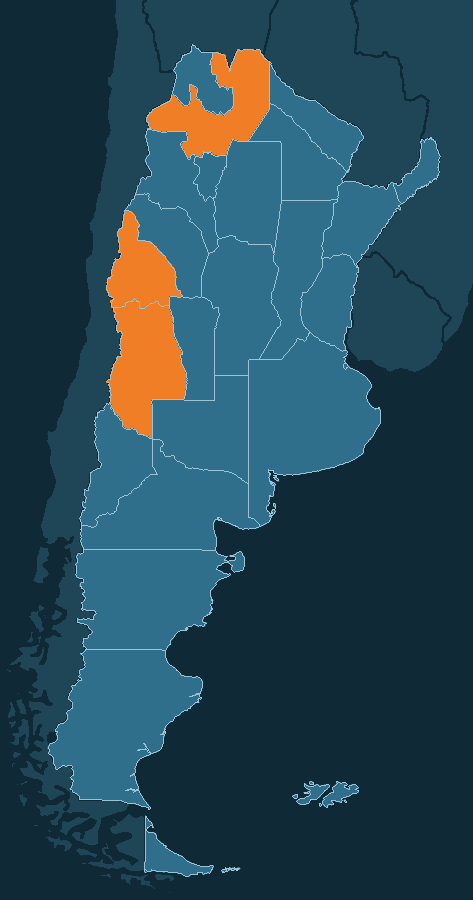
\includegraphics[height=\mapH]{generadas/mapa_argentina.pdf}};}

% Mapa de Sudamérica (scripts/mapa_sudamerica.py): lon -82..-32, lat -56..6
\newlength{\mapSAH}\newlength{\mapSAW}
\newcommand{\geoSA}[2]{({(#1+82)/50*\mapSAW},{(#2+56)/62*\mapSAH})}
\newcommand{\mapaSA}[1]{%
  \setlength{\mapSAH}{#1}\setlength{\mapSAW}{0.73089\mapSAH}%
  \node[anchor=south west, inner sep=0pt] at (0,0)
    {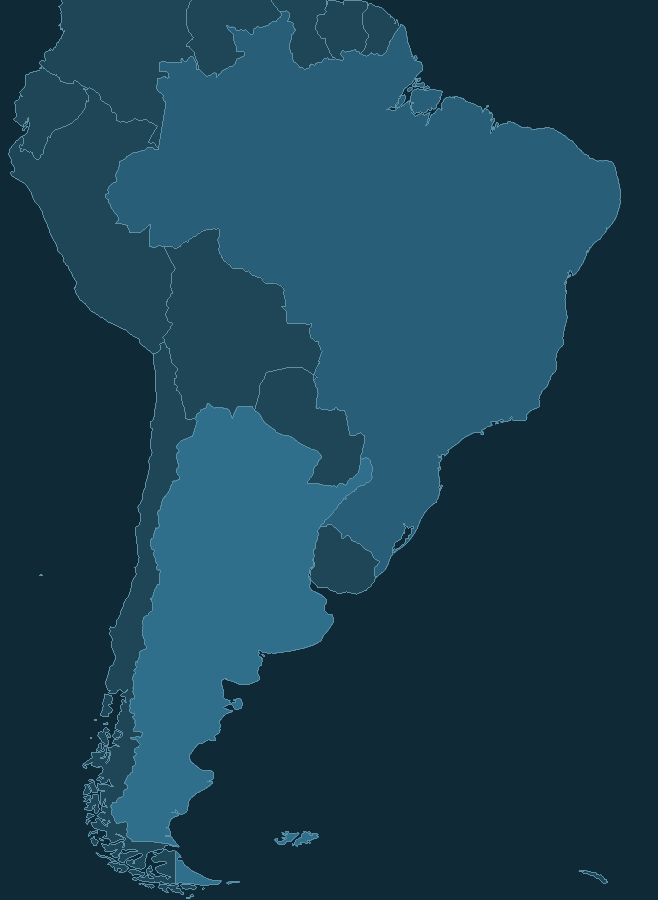
\includegraphics[height=\mapSAH]{generadas/mapa_sudamerica.pdf}};}

% Estilos de PGFPlots coherentes con la paleta
\pgfplotsset{
  coloquio/.style={
    axis line style={itedaGray}, tick style={itedaGray},
    every tick label/.append style={font=\scriptsize, text=itedaTealDark},
    label style={font=\footnotesize, text=itedaTealDark},
    legend style={font=\scriptsize, draw=none, fill=white, fill opacity=0.85,
      text opacity=1},
    /pgf/number format/use comma, /pgf/number format/1000 sep={},
    clip mode=individual,
    grid style={itedaGray!18}, major grid style={itedaGray!18},
  }}

% Flechas y nodos frecuentes
\tikzset{
  flecha/.style={-{Stealth[length=2.2mm]}, thick},
  foton/.style={decorate, decoration={snake, amplitude=0.6mm,
    segment length=2mm, post length=1.5mm}, -{Stealth[length=1.8mm]}},
  etiqueta/.style={font=\footnotesize, text=itedaTealDark},
}


\title{Huellas del universo}
\subtitle{Rayos cósmicos, cosmología y neutrinos desde Argentina}
\author{Lautaro Silva Pizzi}
\institute{ITeDA (CNEA--CONICET--UNSAM)}
\date{Coloquio --- octubre de 2026}

\begin{document}

% ======================================================================
% BLOQUE 0 — Portada y hoja de ruta
% ======================================================================
\bloque{}

% ---------------------------------------------------------------- 1
% Logo de la FIFA (Federación Interuniversitaria de Físicos Argentinos):
% se incluye automáticamente si existe figures/logos/logo_fifa.png
\begin{frame}[plain]
  \fondo[0.10]{halzen/halzen_p005_sintexto.jpg}
  \velo[0.85]{b}
  \begin{tikzpicture}[remember picture, overlay]
    \node[anchor=north west, text=white, font=\small\bfseries, fill=itedaOrange,
      rounded corners=2pt, inner sep=4pt]
      at ([xshift=0.9cm, yshift=-0.6cm]current page.north west)
      {CasiCasiColoquios \;·\; UBA};
    \node[anchor=south west, align=left, text=white, inner sep=0pt]
      at ([xshift=0.9cm, yshift=1.05cm]current page.south west) {%
      {\fontsize{34}{38}\selectfont\bfseries Huellas del universo}\\[5pt]
      {\large\color{itedaOrange}\bfseries Rayos cósmicos, cosmología y
        neutrinos desde Argentina}\\[12pt]
      {\normalsize Lautaro Silva Pizzi}\\[2pt]
      {\small ITeDA (CNEA--CONICET--UNSAM) \quad·\quad FCEN-UBA \quad·\quad octubre de 2026}};
    \node[anchor=south east, fill=white, rounded corners=2pt, inner sep=3pt]
      (logos) at ([xshift=-0.6cm, yshift=1.05cm]current page.south east) {%
      
\includegraphics[height=0.95cm]{logos/logo_uba.png}\hspace{6pt}%
      
\includegraphics[height=0.95cm]{logos/logo-portada5-iteda.png}};
    % FIFA (Federación Interuniversitaria de Físicos Argentinos): arriba a la derecha
    \node[anchor=north east, inner sep=0pt] at ([xshift=-0.6cm, yshift=-0.45cm]current page.north east)
      {
\includegraphics[height=1.9cm]{logos/logo_fifa.png}};
  \end{tikzpicture}
  \creditoblanco{Composición de fondo: F.~Halzen, \textit{IceCube: the first decade of neutrino astronomy}, Erice 2024}
\end{frame}

% Paso de la hoja de ruta: #1 color, #2 mensajero, #3 pregunta, #4 experimento
\newcommand{\paso}[4]{%
  \begin{tikzpicture}
    \node[fill=#1, text=white, font=\bfseries\small, minimum width=2.05cm,
      minimum height=1.15cm, align=center, rounded corners=2pt] (a) {#2};
    \node[right=0.22cm of a, text width=7.15cm, align=left,
      font=\small] {\hyphenpenalty=10000\exhyphenpenalty=10000
      #3\\[-1pt]{\footnotesize\color{itedaGray}#4}};
  \end{tikzpicture}\par\vspace{3.5pt}}

% ---------------------------------------------------------------- 2
\begin{frame}{Cuatro huellas, un mismo cielo}
  \begin{columns}[T,onlytextwidth]
    \column{0.31\textwidth}
      \centering
      \begin{tikzpicture}
        \mapabase{6.55cm}
        % ITeDA
        \fill[white] \geo{-58.52}{-34.57} circle (1.6pt);
        \node[font=\tiny\bfseries, text=white, anchor=north]
          at \geo{-59.5}{-35.0} {ITeDA};
        % Proyectos
        \tikzset{proyecto/.style={fill=itedaTealDark, draw=white, line width=1.1pt},
          every node/.append style={fill=noche, fill opacity=0.75, text opacity=1,
            inner sep=1.2pt, rounded corners=1pt}}
        \filldraw[proyecto] \geo{-66.48}{-24.19} circle (3pt);
        \node[font=\scriptsize\bfseries, text=white, anchor=west]
          at \geo{-65.0}{-24.0} {QUBIC};
        \filldraw[proyecto] \geo{-67.8}{-30.6} circle (3pt);
        \node[font=\scriptsize\bfseries, text=white, anchor=west]
          at \geo{-66.3}{-30.5} {HERON};
        \filldraw[proyecto] \geo{-69.25}{-35.25} circle (3pt);
        \node[font=\scriptsize\bfseries, text=white, anchor=west]
          at \geo{-67.7}{-35.9} {Pierre Auger};
        \draw[white, -{Stealth}, thick] \geo{-64}{-51} -- \geo{-64}{-55.3}
          node[pos=0, above, font=\tiny\bfseries, align=center]
          {IceCube\\Polo Sur};
      \end{tikzpicture}
    \column{0.66\textwidth}
      \vspace{-2pt}
      \paso{cmbAzul}{Luz de 380.000\\años post\\Big Bang}
        {\textbf{¿Cómo era el universo temprano?}}
        {Fondo cósmico de microondas y su polarización \;→\; QUBIC, Salta}
      \paso{itedaOrange}{Núcleos de\\$10^{20}$\,eV}
        {\textbf{¿Qué acelera partículas a energías macroscópicas?}}
        {Lluvias atmosféricas \;→\; Observatorio Pierre Auger, Mendoza}
      \paso{itedaTeal}{Muones\\bajo tierra}
        {\textbf{¿Qué medimos realmente cuando detectamos?}}
        {Mi tesis de licenciatura con el detector subterráneo de muones}
      \paso{violetaNu}{Neutrinos}
        {\textbf{¿Dónde están las fuentes?}}
        {IceCube (Polo Sur) \;→\; HERON, San Juan}
  \end{columns}
  \creditoizq{Mapa: Natural Earth (dominio público)}
\end{frame}

% ======================================================================
% BLOQUE 1 — El universo temprano, el CMB y QUBIC
% ======================================================================
\section{Universo temprano y QUBIC}
\bloque{COSMOLOGÍA}

% ---------------------------------------------------------------- 3
\begin{frame}{Un universo que se enfría al expandirse}
  \begin{columns}[c,onlytextwidth]
    \column{0.64\textwidth}
    \begin{tikzpicture}
      \begin{loglogaxis}[coloquio, width=\linewidth, height=6.0cm,
        xmin=1e-12, xmax=3e18, ymin=0.1, ymax=1e17,
        xlabel={tiempo desde el Big Bang [s]},
        ylabel={temperatura de la radiación [K]},
        xtick={1e-12,1e-8,1e-4,1,1e4,1e8,1e12,1e16},
        ytick={1,1e4,1e8,1e12,1e16}, grid=major]
        \addplot[very thick, itedaTeal, mark=none] coordinates {
          (1e-12,4.7e15) (1e-11,1.5e15) (2e-5,1.8e12) (1,1e10) (180,8e8)
          (1.6e12,9.3e3) (1.2e13,2970) (2.2e16,23.7) (4.35e17,2.7255)};
        \addplot[only marks, mark=*, mark size=2.3pt, itedaOrange] coordinates {
          (1e-11,1.5e15) (2e-5,1.8e12) (180,8e8) (1.2e13,2970) (4.35e17,2.7255)};
        \node[etiqueta, anchor=south west] at (axis cs:2e-11,1.6e15)
          {\scriptsize ruptura electrodébil ($10^{-11}$\,s)};
        \node[etiqueta, anchor=south west] at (axis cs:4e-5,1.9e12)
          {\scriptsize se forman protones y neutrones};
        \node[etiqueta, anchor=south west] at (axis cs:400,8e8)
          {\scriptsize nucleosíntesis: H, He};
        \draw[itedaOrange, thick] (axis cs:1.2e13,2970) -- (axis cs:1e8,1e5);
        \node[font=\scriptsize\bfseries, text=itedaOrange, anchor=east, align=right]
          at (axis cs:1e8,1e5) {CMB: 380.000 años, $\approx$3000\,K};
        \draw[itedaTealDark, thick] (axis cs:4.35e17,2.7255) -- (axis cs:1e9,3);
        \node[font=\scriptsize\bfseries, text=itedaTealDark, anchor=east, fill=white, inner sep=1pt]
          at (axis cs:1e9,3) {hoy: 2,7\,K, 13.800 millones de años};
      \end{loglogaxis}
    \end{tikzpicture}
    \column{0.33\textwidth}
      \small
      La expansión \textbf{estira la longitud de onda} de cada fotón: la
      radiación se enfría como la inversa del tamaño del universo.
      \vspace{2pt}
      \begin{clave}
        Hasta los 380.000 años, materia y luz están en equilibrio: es la
        temperatura \textbf{de todo}. Después, es la de los fotones del CMB.
      \end{clave}
      \vspace{4pt}

      \esquematico\\[-1pt]{\tiny\color{itedaGray} órdenes de magnitud}
  \end{columns}
\end{frame}

% ---------------------------------------------------------------- 4
\begin{frame}{Un plasma opaco}
  \begin{columns}[T,onlytextwidth]
    \column{0.58\textwidth}
    \vspace{4pt}
    \begin{tikzpicture}[x=1cm,y=1cm]
      \begin{scope}
        \fill[itedaOrange!12, rounded corners=3pt] (0,0) rectangle (3.7,3.4);
        \pgfmathsetseed{11}
        \foreach \i in {1,...,32}{
          \pgfmathsetmacro{\px}{0.2+3.3*rnd}\pgfmathsetmacro{\py}{0.2+3.0*rnd}
          \fill[cmbAzul] (\px,\py) circle (1.3pt);}
        \foreach \i in {1,...,28}{
          \pgfmathsetmacro{\px}{0.2+3.3*rnd}\pgfmathsetmacro{\py}{0.2+3.0*rnd}
          \fill[cmbRojo] (\px,\py) circle (2.0pt);}
        \draw[itedaOrange, very thick, -{Stealth}, rounded corners=1pt]
          (0.3,1.8) -- (0.85,2.4) -- (1.15,1.5) -- (1.8,1.9) -- (1.5,2.85)
          -- (2.35,3.0) -- (2.6,2.0) -- (2.05,1.1) -- (2.9,0.7) -- (3.25,1.6);
        \node[font=\small\bfseries, anchor=south, align=center] at (1.85,3.45)
          {antes de 380.000 años};
        \node[font=\scriptsize, text=itedaGray, anchor=north, align=center] at (1.85,-0.05)
          {plasma de $e^-$ y núcleos:\\el fotón rebota sin parar};
      \end{scope}
      \begin{scope}[xshift=4.1cm]
        \fill[cmbAzul!10, rounded corners=3pt] (0,0) rectangle (3.7,3.4);
        \pgfmathsetseed{5}
        \foreach \i in {1,...,24}{
          \pgfmathsetmacro{\px}{0.25+3.2*rnd}\pgfmathsetmacro{\py}{0.25+2.9*rnd}
          \draw[cmbAzul!70] (\px,\py) circle (3.2pt);
          \fill[cmbRojo] (\px,\py) circle (1.4pt);}
        \draw[foton, itedaOrange, very thick] (0.2,2.8) -- (3.6,2.8);
        \draw[foton, itedaOrange, very thick] (0.2,1.7) -- (3.6,1.7);
        \draw[foton, itedaOrange, very thick] (0.2,0.6) -- (3.6,0.6);
        \node[font=\small\bfseries, anchor=south] at (1.85,3.45)
          {después};
        \node[font=\scriptsize, text=itedaGray, anchor=north, align=center] at (1.85,-0.05)
          {átomos neutros:\\el fotón viaja libre hasta hoy};
      \end{scope}
      \node[font=\scriptsize, anchor=west] at (0,-1.0) {\textcolor{cmbAzul}{$\bullet$} electrón
        \quad \textcolor{cmbRojo}{$\bullet$} protón \quad
        \textcolor{cmbAzul!70}{$\circ$} átomo de hidrógeno};
    \end{tikzpicture}
    \column{0.39\textwidth}
      \small
      Los fotones chocan con los electrones libres:\\[4pt]
      \cifra{$\sim$5.000 años luz}{camino libre medio de un fotón\\poco antes de los 380.000 años}\\[4pt]
      \cifra{$\sim$600.000 años luz}{tamaño del universo observable entonces}\\[4pt]
      \begin{clave}
        A $\sim$3000\,K se forman átomos y los fotones \textbf{se desacoplan}:
        lo más lejos que podemos ver con luz.
      \end{clave}
  \end{columns}
\end{frame}

% ---------------------------------------------------------------- 5
\begin{frame}[plain]
  \begin{tikzpicture}[remember picture, overlay]
    \fill[noche] (current page.south west) rectangle (current page.north east);
    \node[inner sep=0pt] at ([yshift=-0.1cm]current page.center)
      {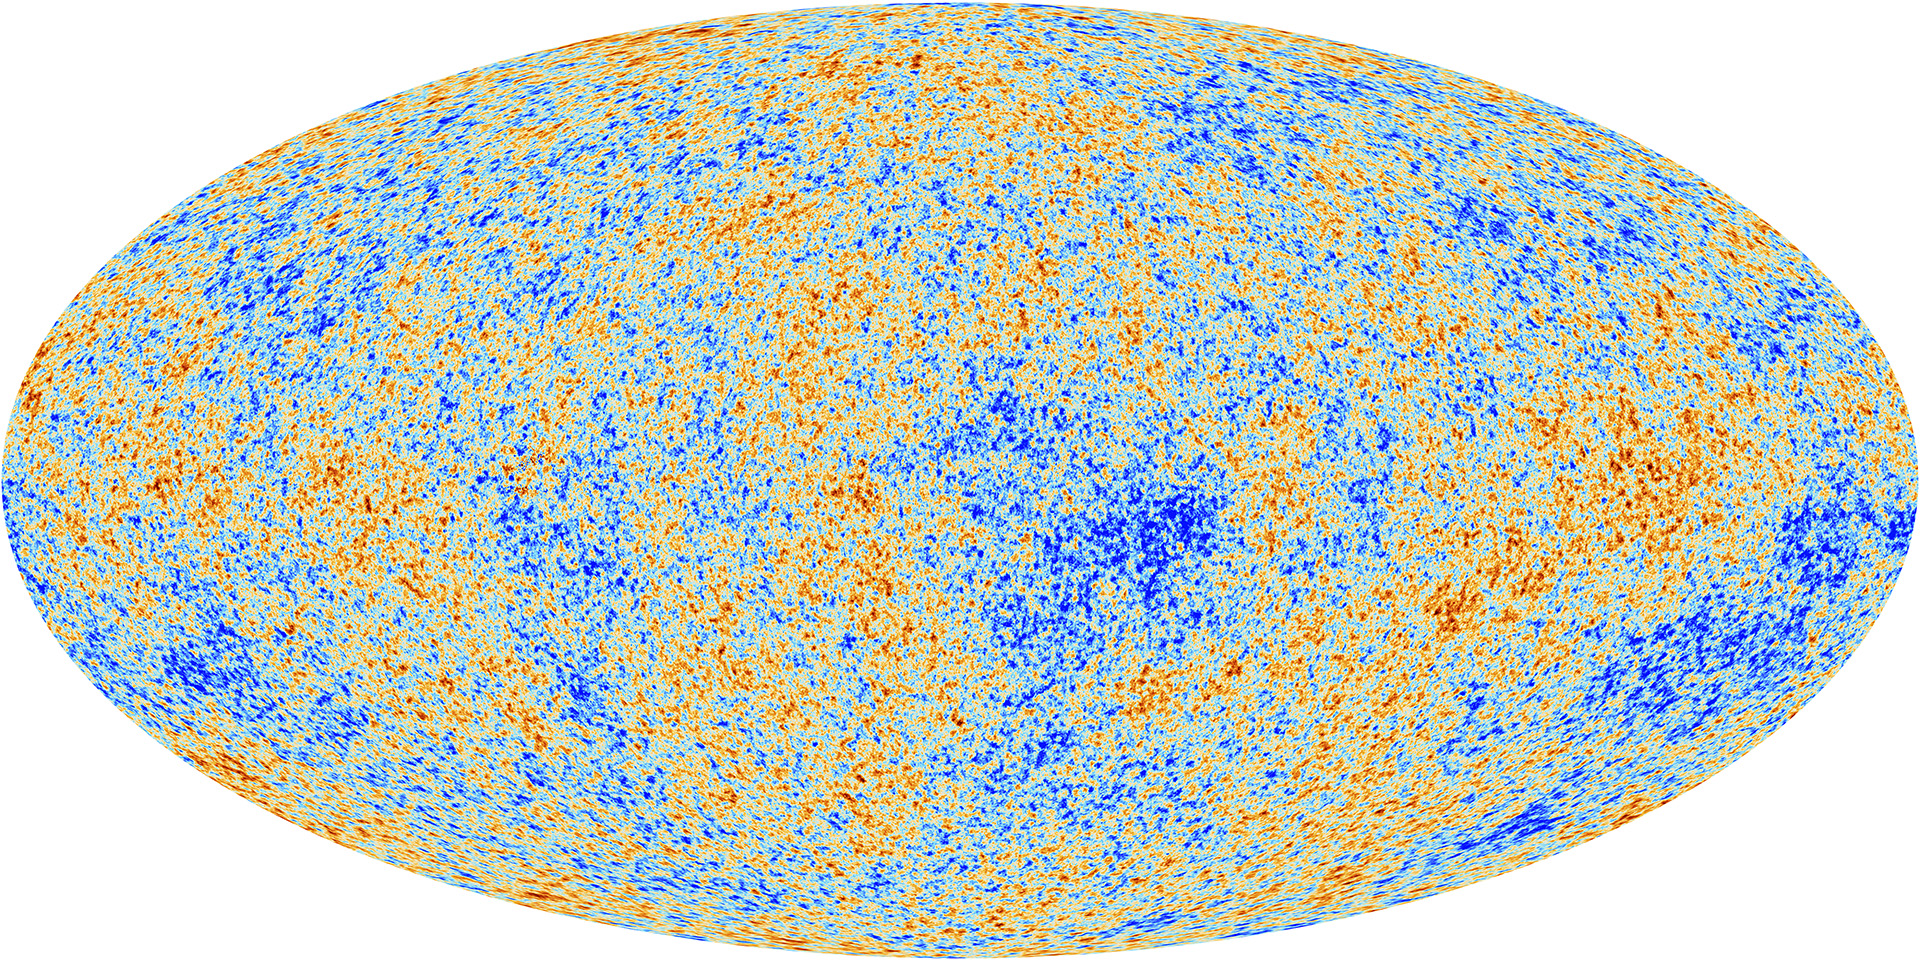
\includegraphics[width=0.78\paperwidth]{externas/planck_cmb_2013.jpg}};
    \node[anchor=north west, text=white, font=\Large\bfseries]
      at ([xshift=0.6cm, yshift=-0.35cm]current page.north west)
      {La fotografía más antigua del universo};
    \node[anchor=south, text=white, font=\small]
      at ([yshift=0.42cm]current page.south)
      {$T_0 = 2{,}7255$\,K \quad · \quad
       \textcolor{itedaOrange}{manchas de $\pm$1 parte en 100.000} \quad · \quad
       380.000 años post Big Bang};
  \end{tikzpicture}
  \creditoblanco{ESA y Colaboración Planck (2013)}
\end{frame}

% ---------------------------------------------------------------- 6
\begin{frame}{El cuerpo negro más perfecto que conocemos}
  \begin{columns}[c,onlytextwidth]
    \column{0.56\textwidth}
    \begin{tikzpicture}
      \begin{axis}[coloquio, name=main, width=\linewidth, height=4.5cm,
        xmin=40, xmax=680, ymin=0, ymax=420, xticklabels={},
        ylabel={brillo [MJy/sr]}, grid=major]
        \addplot[thick, itedaTeal] table[x=nu_GHz, y=I_MJysr] {data/planck_2725K.dat};
        \addlegendentry{cuerpo negro de 2,725\,K}
        \addplot[only marks, mark=*, mark size=1.4pt, itedaOrange]
          table[x=nu_GHz, y=I_MJysr] {data/firas.dat};
        \addlegendentry{medición de COBE/FIRAS}
      \end{axis}
      \begin{axis}[coloquio, at={(main.south west)}, anchor=north west,
        yshift=-0.1cm, width=\linewidth, height=2.7cm, xmin=40, xmax=680,
        ymin=-70, ymax=70, xlabel={frecuencia [GHz]},
        ylabel={dato $-$ curva}, grid=major, ytick={-50,0,50}]
        \addplot[thin, itedaGray] coordinates {(40,0) (680,0)};
        \addplot[only marks, mark=*, mark size=1.1pt, itedaOrange,
          error bars/.cd, y dir=both, y explicit]
          table[x=nu_GHz, y=resid_kJysr, y error=sigma_kJysr] {data/firas.dat};
      \end{axis}
    \end{tikzpicture}
    \column{0.41\textwidth}
      \small
      \textbf{Arriba}: el brillo del cielo en microondas, frecuencia por
      frecuencia. Los puntos caen \textbf{exactamente} sobre la curva de un
      cuerpo negro.
      \vspace{4pt}

      \textbf{Abajo}: lo que sobra al restar la curva, en unidades 1000
      veces más chicas: menos de \textbf{1 parte en 10.000}.
      \vspace{4pt}
      \begin{clave}
        Se emitió a $\sim$3000\,K. La expansión lo enfrió $\sim$1100 veces
        sin cambiarle la forma: el universo estuvo \textbf{caliente y en
        equilibrio}.
      \end{clave}
  \end{columns}
  \credito{Datos: Fixsen \textit{et al.}, ApJ 473 (1996) 576 (NASA LAMBDA)}
\end{frame}

% ---------------------------------------------------------------- 7
\begin{frame}{Las manchas del CMB y nuestro modelo del universo}
  \begin{columns}[c,onlytextwidth]
    \column{0.60\textwidth}
    \begin{tikzpicture}
      \begin{semilogxaxis}[coloquio, width=\linewidth, height=6.0cm,
        xmin=2, xmax=2500, ymin=0, ymax=7400,
        xlabel={multipolo $\ell$ \quad (tamaño angular $\approx 180^\circ/\ell$)},
        ylabel={amplitud de las manchas [$\mu$K$^2$]},
        xtick={2,10,100,1000}, xticklabels={2,10,100,1000},
        extra x ticks={2,18,180,1800}, extra x tick labels={$90^\circ$,$10^\circ$,$1^\circ$,$0{,}1^\circ$},
        extra x tick style={tick label style={yshift=5.5cm, text=itedaGray}, grid=none},
        grid=major, legend style={at={(0.99,0.98)}, anchor=north east}]
        \fill[cmbAzul!10] (axis cs:2,0) rectangle (axis cs:30,7400);
        \fill[itedaOrange!12] (axis cs:30,0) rectangle (axis cs:400,7400);
        \fill[verdeRadio!10] (axis cs:400,0) rectangle (axis cs:2500,7400);
        \addplot[thick, itedaTeal] table[x=ell, y=TT] {data/planck_theory.dat};
        \addlegendentry{modelo $\Lambda$CDM}
        \addplot[only marks, mark=*, mark size=1.0pt, cmbRojo,
          error bars/.cd, y dir=both, y explicit]
          table[x=ell, y=Dl, y error plus=errhi, y error minus=errlo]
          {data/planck_tt_binned.dat};
        \addlegendentry{Planck 2018}
        \addplot[only marks, mark=*, mark size=1.0pt, cmbRojo, forget plot,
          error bars/.cd, y dir=both, y explicit]
          table[x=ell, y=Dl, y error plus=errhi, y error minus=errlo]
          {data/planck_tt_lowl.dat};
        \node[circle, fill=cmbAzul, text=white, font=\scriptsize\bfseries, inner sep=1.5pt] at (axis cs:7,4500) {1};
        \node[circle, fill=itedaOrange, text=white, font=\scriptsize\bfseries, inner sep=1.5pt] at (axis cs:110,4500) {2};
        \node[circle, fill=verdeRadio, text=white, font=\scriptsize\bfseries, inner sep=1.5pt] at (axis cs:900,4500) {3};
      \end{semilogxaxis}
    \end{tikzpicture}
    \column{0.37\textwidth}
      \footnotesize
      \textbf{\color{cmbAzul}1 · Manchas grandes}: las fluctuaciones
      primordiales tal como nacieron.\\[4pt]
      \textbf{\color{itedaOrange}2 · Primer pico ($\sim$1$^\circ$)}: ondas de
      sonido del plasma. Su tamaño dice que el universo es \textbf{plano}.\\[4pt]
      \textbf{\color{verdeRadio}3 · Picos siguientes}: cuánta materia
      ordinaria y oscura hay. A escalas chicas se borran.\\[6pt]
      \begin{clave}
        Un modelo con \textbf{6 parámetros} ---materia oscura fría y energía
        oscura--- ajusta todos los puntos.
      \end{clave}
  \end{columns}
  \credito{Datos: Planck 2018 (PR3), Planck Legacy Archive / IRSA}
\end{frame}

% ---------------------------------------------------------------- 8
\begin{frame}{Polarización: la huella de las ondas gravitacionales}
  \begin{columns}[T,onlytextwidth]
    \column{0.33\textwidth}
      \centering
      \begin{tikzpicture}[scale=0.85]
        \draw[cmbRojo, line width=2.4pt, -{Stealth[length=3mm]}] (-1.9,0) -- (-0.35,0);
        \draw[cmbRojo, line width=2.4pt, -{Stealth[length=3mm]}] (1.9,0) -- (0.35,0);
        \draw[cmbAzul, line width=0.9pt, -{Stealth[length=2mm]}] (0,1.9) -- (0,0.35);
        \draw[cmbAzul, line width=0.9pt, -{Stealth[length=2mm]}] (0,-1.9) -- (0,-0.35);
        \shade[ball color=itedaTeal] (0,0) circle (0.22);
        \node[font=\scriptsize\bfseries, white] at (0,0) {$e^-$};
        \node[font=\scriptsize, text=cmbRojo] at (-1.35,0.3) {caliente};
        \node[font=\scriptsize, text=cmbAzul] at (0.5,1.5) {frío};
        \draw[itedaOrange, line width=1.6pt, {Stealth}-{Stealth}] (0.75,-1.15) -- (1.85,-1.15);
        \node[font=\scriptsize, align=center] at (1.3,-1.6) {sale polarizada};
      \end{tikzpicture}\\[3pt]
      {\footnotesize Un electrón que recibe más luz de un eje que del otro
      (\textbf{cuadrupolo}) la reemite polarizada.}
    \column{0.33\textwidth}
      \centering
      \begin{tikzpicture}[scale=0.58]
        \foreach \r in {0.75,1.45}{
          \foreach \a in {0,30,...,330}{
            \draw[itedaTeal, line width=1.1pt] ({\r*cos(\a)-0.22*cos(\a)},{\r*sin(\a)-0.22*sin(\a)})
              -- ({\r*cos(\a)+0.22*cos(\a)},{\r*sin(\a)+0.22*sin(\a)});}}
        \node[font=\small\bfseries] at (0,-2.15) {modo E};
        \begin{scope}[xshift=3.6cm]
        \foreach \r in {0.75,1.45}{
          \foreach \a in {0,30,...,330}{
            \pgfmathsetmacro{\b}{\a+45}
            \draw[violetaNu, line width=1.1pt] ({\r*cos(\a)-0.22*cos(\b)},{\r*sin(\a)-0.22*sin(\b)})
              -- ({\r*cos(\a)+0.22*cos(\b)},{\r*sin(\a)+0.22*sin(\b)});}}
        \node[font=\small\bfseries] at (0,-2.15) {modo B};
        \end{scope}
      \end{tikzpicture}\\[4pt]
      {\footnotesize Dos patrones: E (radial) y B (remolino).
      Las fluctuaciones de \textbf{densidad} sólo producen E.}
    \column{0.30\textwidth}
      \small
      El cuadrupolo sólo existe \textbf{cerca de la última dispersión}: la
      polarización es una foto de ese instante.
      \vspace{2pt}
      \begin{clave}
        Los \textbf{modos B} primordiales serían la huella de \textbf{ondas
        gravitacionales} del período inflacionario.
      \end{clave}
      {\scriptsize\color{itedaGray} Aún no detectados.}
  \end{columns}
\end{frame}

% ---------------------------------------------------------------- 9
\bloque{COSMOLOGÍA · QUBIC}
\begin{frame}{QUBIC: cosmología a casi 5.000 m en la Puna salteña}
  \begin{columns}[T,onlytextwidth]
    \column{0.44\textwidth}
      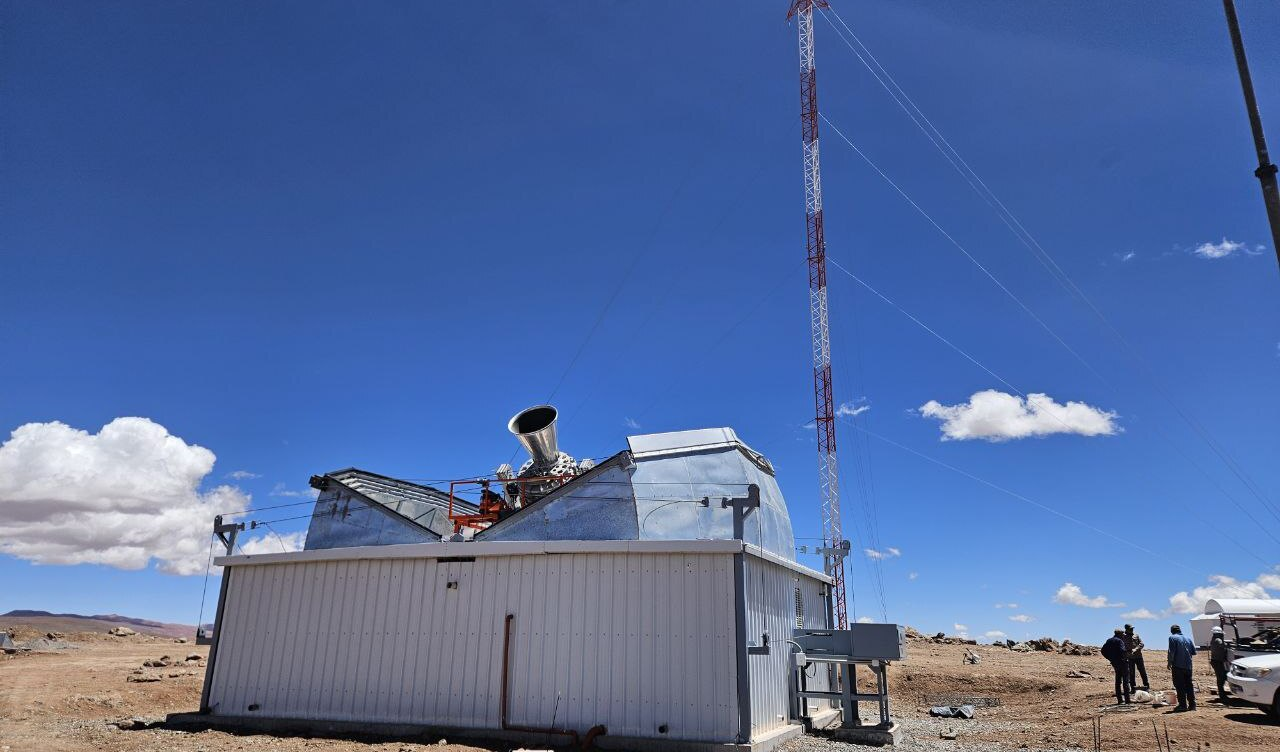
\includegraphics[width=0.9\linewidth]{qubic/qubic_cupula_r17.jpg}\\[2pt]
      \begin{tikzpicture}
        \node[inner sep=0pt, anchor=south west] (a) at (0,0)
          {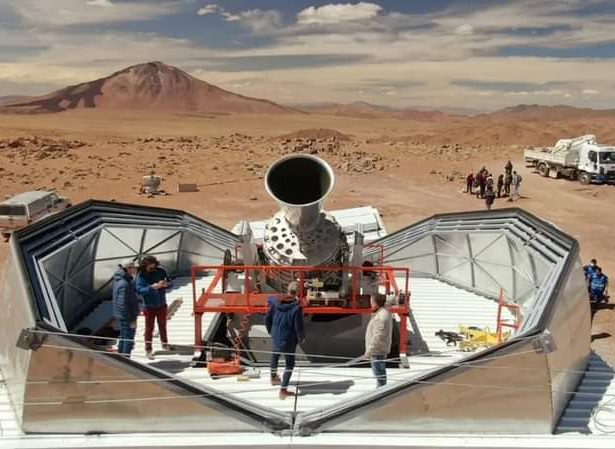
\includegraphics[width=0.445\linewidth]{qubic/qubic_e2_cupula_abierta_r.jpg}};
        \node[inner sep=0pt, anchor=south west] (b) at ([xshift=2pt]a.south east)
          {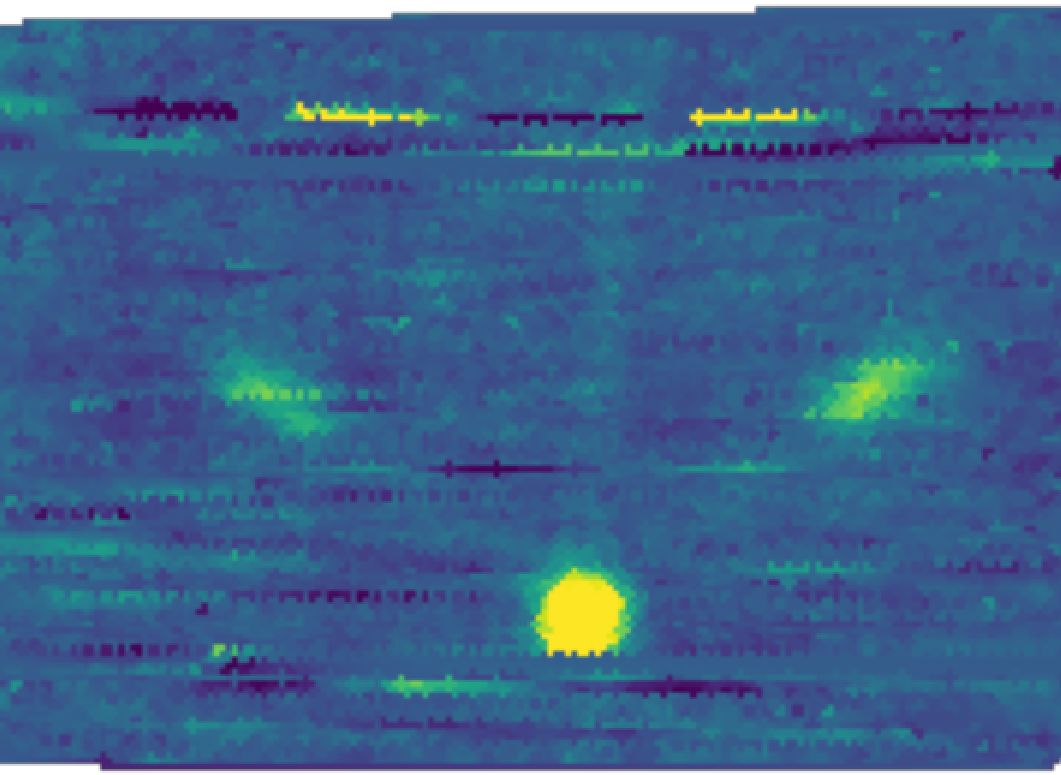
\includegraphics[width=0.445\linewidth]{qubic/qubic_luna_2026_r.png}};
        \node[anchor=south east, font=\tiny, text=white, fill=black, fill opacity=0.55,
          text opacity=1, inner sep=1.5pt] at (b.south east) {Luna, 11/03/2026};
      \end{tikzpicture}
    \column{0.53\textwidth}
      \small
      \textbf{Q\&U Bolometric Interferometer for Cosmology}: busca los modos B
      primordiales a 150 y 220\,GHz.
      \begin{itemize}\footnotesize
        \item \textbf{Alto Chorrillos}, cerca de San Antonio de los Cobres. El
          vapor de agua absorbe microondas: a esa altura el aire es muy seco.
        \item Seis países: Argentina, Francia, Irlanda, Italia, Reino Unido y EE.\,UU.
        \item \textbf{ITeDA}: infraestructura y montura, análisis de datos,
          nuevos sensores.
      \end{itemize}
      \vspace{3pt}
      \begin{tikzpicture}[x=1cm]
        \draw[itedaGray, thick] (-0.2,0) -- (7.6,0);
        \foreach \x/\y/\t in {0.2/2021/{llega a\\Salta}, 1.75/2022/{instalación\\en el sitio},
          3.3/2024/{torre de\\calibración}, 4.85/2025/{montura\\completa}, 6.6/2026/{primer barrido\\de la Luna}}{
          \fill[itedaOrange] (\x,0) circle (2.2pt);
          \node[font=\scriptsize\bfseries, above] at (\x,0.05) {\y};
          \node[font=\tiny, below, align=center] at (\x,-0.05) {\t};}
      \end{tikzpicture}
  \end{columns}
  \creditoizq{Fotos: F.~Sánchez, CLAF--CNRS (abr.\ 2026); L.~Silva Pizzi, Final de Estructura de la Materia 2 (2026)}
\end{frame}

% ---------------------------------------------------------------- 10
\begin{frame}{El desafío: una parte en cien millones}
  \begin{columns}[c,onlytextwidth]
    \column{0.47\textwidth}
    \begin{tikzpicture}
      \begin{loglogaxis}[coloquio, width=\linewidth, height=5.6cm,
        xmin=2, xmax=2500, ymin=0.005, ymax=200,
        xlabel={multipolo $\ell$}, ylabel={amplitud [$\mu$K]},
        xtick={10,100,1000}, xticklabels={10,100,1000},
        ytick={0.01,0.1,1,10,100}, yticklabels={{0,01},{0,1},1,10,100},
        grid=major]
        \fill[itedaOrange!14] (axis cs:30,0.005) rectangle (axis cs:200,200);
        \addplot[thick, cmbRojo] table[x=ell, y expr=sqrt(\thisrow{TT})] {data/planck_theory.dat};
        \addplot[thick, itedaTeal] table[x=ell, y expr=sqrt(\thisrow{EE})] {data/planck_theory.dat};
        \addplot[thick, violetaNu] table[x=ell, y expr=sqrt(\thisrow{BB})] {data/planck_theory.dat};
        \draw[violetaNu, dashed, thick] (axis cs:20,0.03) -- (axis cs:300,0.03);
        \node[font=\scriptsize, text=violetaNu, anchor=south, align=center]
          at (axis cs:7,0.012) {B primordiales:\\decenas de nK};
        \node[font=\scriptsize\bfseries, text=itedaOrange, anchor=north] at (axis cs:78,160) {QUBIC};
        \node[font=\scriptsize\bfseries, text=cmbRojo, anchor=south west] at (axis cs:2.3,70) {temperatura};
        \node[font=\scriptsize\bfseries, text=itedaTeal] at (axis cs:900,12) {E};
        \node[font=\scriptsize\bfseries, text=violetaNu, anchor=north] at (axis cs:1300,0.2) {B (lente)};
      \end{loglogaxis}
    \end{tikzpicture}
    \column{0.50\textwidth}
      \begin{columns}[T,onlytextwidth]
        \column{0.5\linewidth}
          \cifra{$10^{-8}$}{señal buscada respecto\\de lo que llega}\\[6pt]
          \cifra{$\sim$$10^{9}$}{fotones del CMB por\\segundo en cada detector}
        \column{0.5\linewidth}
          \cifra{0,6\,meV}{energía de cada fotón\\(3000 veces menos que el visible)}\\[6pt]
          \cifra{$10^{-20}$\,W}{diferencia de potencia\\a distinguir}
      \end{columns}
      \vspace{6pt}
      \begin{clave}
        No se cuentan fotones: se mide \textbf{potencia}, con miles de
        detectores muy fríos y años de integración.
      \end{clave}
  \end{columns}
  \credito{Espectros: Planck 2018, mejor ajuste $\Lambda$CDM (sin componente tensorial)}
\end{frame}

% ---------------------------------------------------------------- 11
\begin{frame}{Bolómetros y sensores de borde de transición (TES)}
  \begin{columns}[c,onlytextwidth]
    \column{0.45\textwidth}
      \centering
      \begin{tikzpicture}[x=0.8cm,y=0.8cm]
        \fill[pattern=north east lines, pattern color=itedaGray] (-0.4,-0.55) rectangle (4.4,-0.2);
        \draw[itedaGray, thick] (-0.4,-0.2) -- (4.4,-0.2);
        \node[font=\scriptsize, anchor=north] at (2,-0.6) {baño frío a $\approx$0,3\,K};
        \draw[decorate, decoration={zigzag, amplitude=1.2mm, segment length=2.2mm},
          thick, itedaTeal] (2,-0.2) -- (2,1.2);
        \node[font=\scriptsize, anchor=west, text=itedaTeal, align=left] at (2.25,0.5)
          {vínculo térmico\\débil};
        \draw[thick, fill=itedaOrange!25, rounded corners=1pt] (0.6,1.2) rectangle (3.4,2.0);
        \node[font=\scriptsize] at (1.85,1.6) {absorbente};
        \fill[itedaTealDark] (3.0,1.32) rectangle (3.32,1.48);
        \draw[itedaTealDark] (3.16,1.48) -- (3.9,2.2) node[above, font=\scriptsize] {TES};
        \draw[foton, itedaOrange, thick] (0.4,3.1) -- (1.2,2.1);
        \draw[foton, itedaOrange, thick] (1.5,3.2) -- (1.9,2.1);
        \node[font=\scriptsize, text=itedaOrange, anchor=south] at (0.9,3.15) {luz del cielo};
      \end{tikzpicture}\\[6pt]
      \footnotesize
      \textbf{Bolómetro}: la luz \textbf{calienta} un absorbente unido
      débilmente a un baño frío. Cuánto se calienta mide la potencia.
    \column{0.52\textwidth}
      \begin{tikzpicture}
        \begin{axis}[coloquio, width=\linewidth, height=3.6cm,
          xmin=395, xmax=425, ymin=-0.05, ymax=1.15,
          xlabel={temperatura del sensor [mK]}, ylabel={resistencia},
          grid=major, ytick=\empty]
          \addplot[very thick, itedaTeal, domain=395:425, samples=150]
            {0.5*(1+tanh((x-410)/2.2))};
          \fill[itedaOrange] (axis cs:410.6,0.635) circle (2.5pt);
          \node[font=\scriptsize, text=itedaOrange, anchor=west, align=left]
            at (axis cs:411.8,0.45) {punto de\\operación};
          \node[font=\scriptsize, anchor=south] at (axis cs:401,0.04) {superconductor};
          \node[font=\scriptsize, anchor=north] at (axis cs:420,0.97) {normal};
          \node[font=\scriptsize, text=itedaGray, anchor=south east] at (axis cs:409.5,0.75)
            {$T_c\approx410$\,mK};
        \end{axis}
      \end{tikzpicture}
      \begin{clave}
        \textbf{TES}: un superconductor operado justo \textbf{en su
        transición}, donde la resistencia cambia violentamente con la
        temperatura: un calentamiento ínfimo se vuelve un cambio grande de
        corriente.
      \end{clave}
  \end{columns}
  \creditoizq{Curva ilustrativa. $T_c$ (NbSi): QUBIC IV, arXiv:2101.06787}
\end{frame}

% ---------------------------------------------------------------- 12
\begin{frame}{Cómo se lee un TES: el SQUID}
  \centering
  \begin{tikzpicture}[x=1cm,y=1cm,
    caja/.style={rounded corners=3pt, draw=itedaTeal, fill=itedaLight, thick,
      minimum height=1.2cm, text width=2.15cm, align=center, font=\scriptsize},
    clave/.style={caja, draw=itedaOrange, fill=itedaOrange!12},
    paso/.style={-{Stealth[length=2.4mm]}, very thick, itedaOrange}]
    \node[caja] (luz) at (0,0) {\textbf{Luz del cielo}\\llega más o menos potencia};
    \node[caja] (tes) at (2.9,0) {\textbf{TES}\\se calienta y cambia su resistencia};
    \node[caja] (bob) at (5.8,0) {\textbf{Bobina}\\cambia la corriente y su campo};
    \node[clave] (sq) at (8.7,0) {\textbf{SQUID}\\cambia el flujo y su tensión};
    \node[caja] (asic) at (11.6,0) {\textbf{Electrónica}\\a 40\,K: amplifica y digitaliza};
    \draw[paso] (luz) -- (tes); \draw[paso] (tes) -- (bob);
    \draw[paso] (bob) -- (sq); \draw[paso] (sq) -- (asic);
    \node[font=\tiny, text=itedaGray, below=1pt of tes] {0,3\,K};
    \node[font=\tiny, text=itedaGray, below=1pt of sq] {1\,K};
  \end{tikzpicture}\\[6pt]
  \begin{columns}[c,onlytextwidth]
    \column{0.30\textwidth}
      \centering
      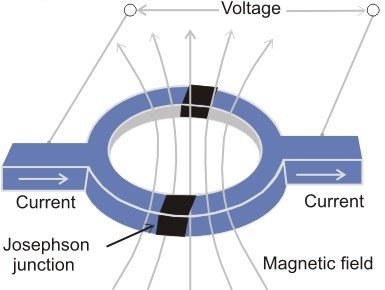
\includegraphics[width=0.72\linewidth]{qubic/squid_e2_esquema.jpg}\\[0pt]
      {\tiny Anillo con dos junturas Josephson}
    \column{0.67\textwidth}
      \footnotesize
      \begin{itemize}\footnotesize
        \item \textbf{Juntura Josephson}: barrera aislante finísima entre dos
          superconductores, que la corriente cruza por \textbf{efecto túnel}.
        \item La corriente se divide en dos ramas; el flujo magnético del
          anillo las \textbf{desfasa} y al juntarse \textbf{interfieren}, como
          en una doble rendija.
      \end{itemize}
      \begin{clave}
        La tensión oscila con período $\Phi_0=h/2e$ (\textbf{cuanto de flujo}):
        un cambio minúsculo de corriente se vuelve medible.
        \textbf{El TES mide, el SQUID lee.}
      \end{clave}

  \end{columns}
\end{frame}

% ---------------------------------------------------------------- 13
\begin{frame}{¿Por qué el detector está más frío que el CMB?}
  \begin{columns}[c,onlytextwidth]
    \column{0.64\textwidth}
      \centering
      \begin{tikzpicture}[x=1cm,y=1cm]
        % termómetro horizontal, escala log: x = 2*log10(T/0.1 K)
        \shade[left color=cmbAzul!70, right color=cmbRojo!70, rounded corners=4pt]
          (0,0) rectangle (7.0,0.35);
        \foreach \t/\x/\l/\c/\up in {
            300/6.95/{300 K\\ambiente}/itedaGray/1,
            77/5.77/{77 K\\nitrógeno líquido}/itedaGray/0,
            4.2/3.25/{4 K\\helio líquido}/itedaGray/1,
            2.725/2.87/{2,7 K\\\textbf{CMB}}/itedaOrange/0,
            0.3/0.95/{0,3 K\\\textbf{detectores}}/itedaTeal/1}{
          \draw[\c, very thick] (\x,-0.05) -- (\x,0.4);
          \ifnum\up=1
            \node[font=\scriptsize, text=\c, align=center, anchor=south] at (\x,0.45) {\l};
          \else
            \node[font=\scriptsize, text=\c, align=center, anchor=north] at (\x,-0.1) {\l};
          \fi}
      \end{tikzpicture}\\[8pt]
      \begin{minipage}{0.96\linewidth}
      \footnotesize
      La temperatura de 2,7\,K describe el \textbf{espectro} de la luz
      (cuánta energía trae), no la temperatura a la que debe estar el
      detector. Hay que enfriarlo porque:
      \begin{enumerate}\footnotesize
        \item el \textbf{ruido térmico} del propio sensor baja con la temperatura;
        \item todo lo que está caliente \textbf{brilla} en microondas: lentes,
          espejos y paredes se enfrían para no tapar al cielo;
        \item la \textbf{transición superconductora} del TES está a $\sim$0,4\,K.
      \end{enumerate}
      \end{minipage}
    \column{0.33\textwidth}
      \centering
      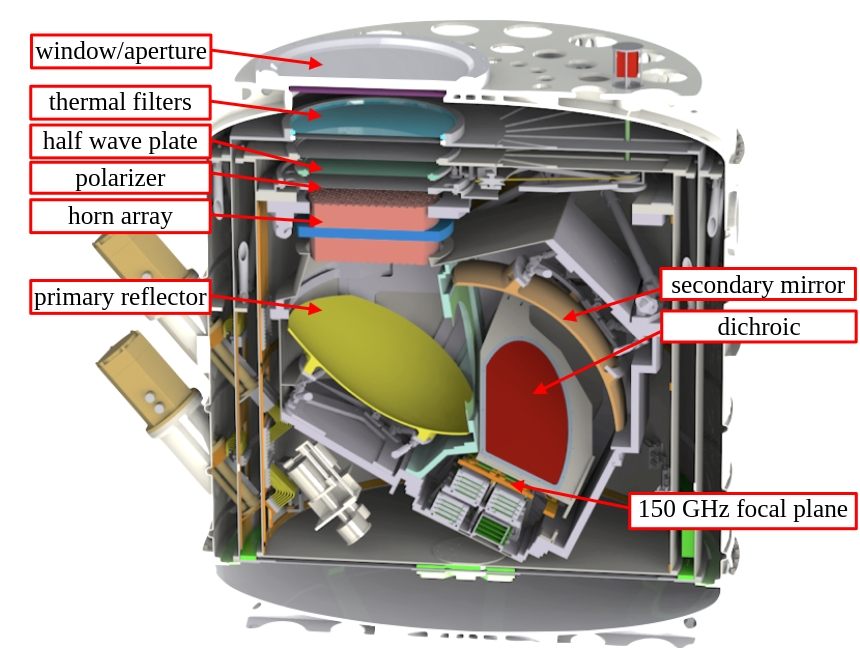
\includegraphics[width=0.7\linewidth]{qubic/qubic_criostato_corte.jpg}\\[2pt]
      {\scriptsize Criostato de QUBIC (1,8\,m $\times$ 1,6\,m): etapas a 40\,K,
      4\,K, 1\,K y 0,3\,K}\\[6pt]
      \begin{clave}
        Un termómetro al sol no está a 5800\,K: \textbf{mide la potencia}
        que le llega.
      \end{clave}
  \end{columns}
  \creditoizq{Corte del criostato: Colaboración QUBIC (vía F.~Sánchez, 2026)}
\end{frame}

% ---------------------------------------------------------------- separador
\bloque{}
\begin{frame}[plain]
  \fondo[0.15]{halzen/cielo_montanas.jpg}
  \velo[0.8]{l}
  \begin{tikzpicture}[remember picture, overlay]
    \node[anchor=west, text=white, align=left, text width=10cm]
      at ([xshift=0.9cm]current page.west) {%
      {\small\color{itedaOrange}\bfseries DE LA LUZ MÁS ANTIGUA\\A LAS PARTÍCULAS MÁS ENERGÉTICAS}\\[8pt]
      {\fontsize{34}{38}\selectfont\bfseries Rayos cósmicos}\\[8pt]
      {\normalsize Aceleradores naturales, el espectro\\y el Observatorio Pierre Auger}};
  \end{tikzpicture}
  \creditoblanco{Foto: vía F.~Halzen, Erice 2024}
\end{frame}

% ======================================================================
% BLOQUE 2 — Rayos cósmicos y astrofísica de altas energías
% ======================================================================
\section{Rayos cósmicos}
\bloque{RAYOS CÓSMICOS}

% ---------------------------------------------------------------- 16
\begin{frame}{Rayos cósmicos: aceleradores naturales}
  \begin{columns}[c,onlytextwidth]
    \column{0.45\textwidth}
      \small
      Descubiertos por V.~Hess en 1912. Los primarios cargados son
      \textbf{núcleos}: $\sim$90\% protones, $\sim$9\% helio, $\sim$1\% más
      pesados, con energías de hasta \textbf{más de $10^{20}$\,eV}.
      \vspace{6pt}

      \centering
      \begin{tikzpicture}[x=1cm,y=1cm]
        \shade[ball color=itedaOrange!70] (0,0) circle (0.25);
        \node[font=\tiny, below=3pt] at (0,-0.25) {fuente};
        \draw[very thick, itedaOrange, -{Stealth}] (0.3,0.05)
          .. controls (1.4,1.2) and (2.0,-1.0) .. (3.0,0.2)
          .. controls (3.6,0.9) and (4.0,0.0) .. (4.6,-0.1);
        \draw[dashed, itedaGray] (0.3,0) -- (4.6,0);
        \shade[ball color=cmbAzul!60] (4.85,-0.1) circle (0.22);
        \node[font=\tiny, below=3pt] at (4.85,-0.32) {Tierra};
        \draw[thick, itedaTealDark, -{Stealth}] (4.6,-0.1) -- ++(-0.9,0.75)
          node[above, font=\tiny, align=center] {dirección\\aparente};
      \end{tikzpicture}\\[4pt]
      \begin{clave}
        Los campos magnéticos de la galaxia y del espacio intergaláctico
        curvan su trayectoria: la dirección de llegada \textbf{no apunta} a la
        fuente.
      \end{clave}
    \column{0.52\textwidth}
      \centering
      \begin{tikzpicture}[x=1cm,y=1cm]
        \tikzset{tarjeta/.style={rounded corners=3pt, minimum width=6.9cm,
          inner sep=4pt, text width=6.6cm, align=left, font=\footnotesize}}
        \node[tarjeta, fill=itedaOrange!15, draw=itedaOrange] at (0,3.2)
          {\textbf{\color{itedaOrange}Núcleos cargados}: llegan muchos, pero
          \textbf{desviados} por campos magnéticos y frenados por los fondos
          de radiación.};
        \node[tarjeta, fill=cmbAzul!12, draw=cmbAzul] at (0,1.6)
          {\textbf{\color{cmbAzul}Fotones gamma}: viajan en línea recta, pero se
          \textbf{absorben} ($\gamma\gamma\to e^+e^-$). A PeV, el horizonte es
          la galaxia.};
        \node[tarjeta, fill=violetaNu!12, draw=violetaNu] at (0,0)
          {\textbf{\color{violetaNu}Neutrinos}: ni se desvían ni se absorben,
          pero casi \textbf{no interactúan}.};
      \end{tikzpicture}
  \end{columns}
\end{frame}

% ---------------------------------------------------------------- 17
\begin{frame}{El espectro de los rayos cósmicos}
  \begin{columns}[c,onlytextwidth]
    \column{0.50\textwidth}
      \centering
      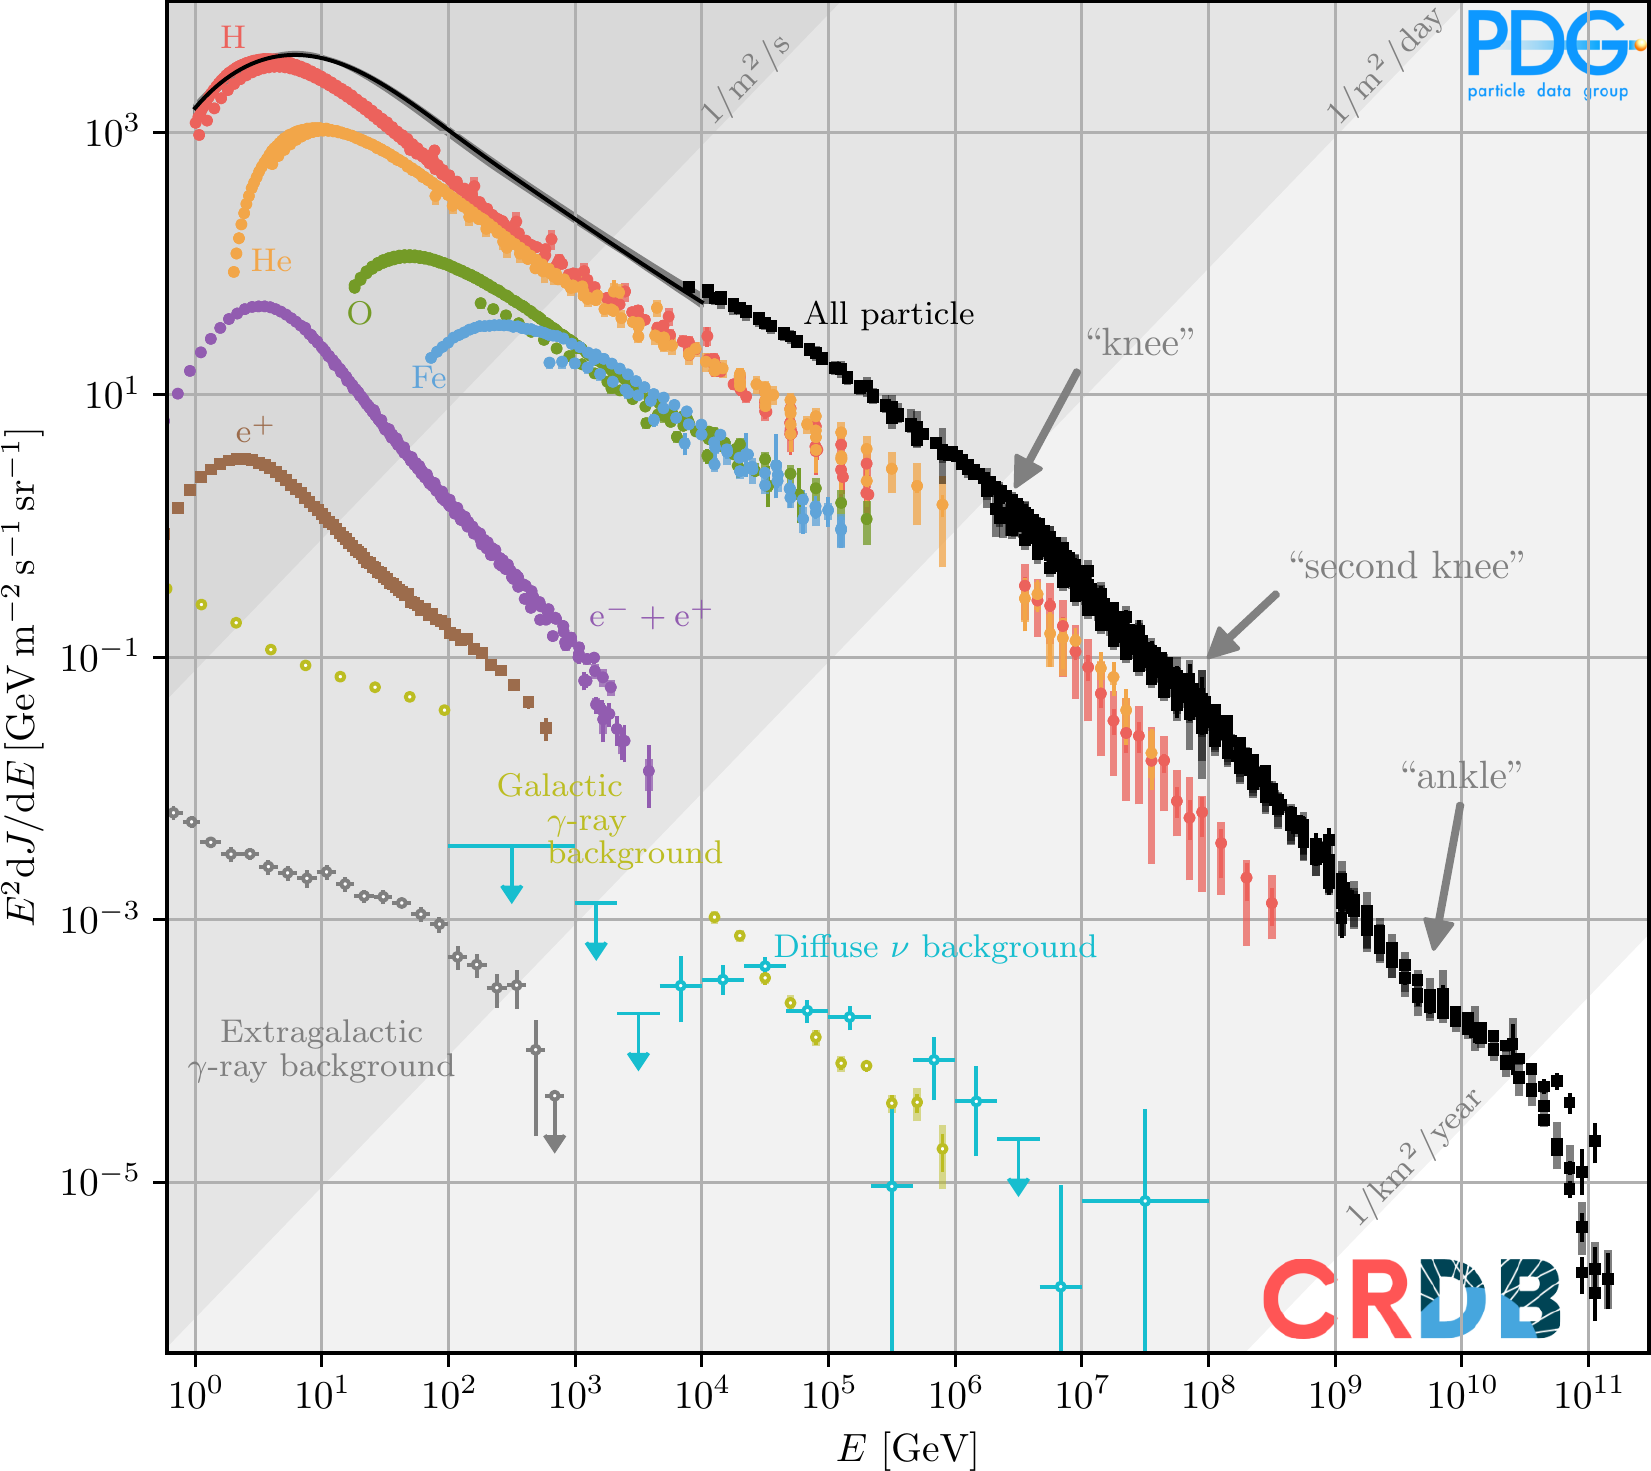
\includegraphics[width=\linewidth]{externas/pdg2024_espectro_E2.png}
    \column{0.47\textwidth}
      \small
      El flujo cae como $E^{-2,7}$: lo que se ve es el flujo
      \textbf{multiplicado por $E^2$}. Las diagonales grises marcan cuántas
      partículas llegan por encima de esa energía:\\[4pt]
      \begin{tikzpicture}
        \foreach \y/\e/\f in {0/{$10^{11}$ eV}/{1 partícula por m$^2$ por segundo},
            -0.5/{$\sim3\times10^{15}$ eV}/{1 por m$^2$ por año (\emph{rodilla})},
            -1.0/{$\sim10^{19}$ eV}/{$\sim$1 por km$^2$ por año},
            -1.5/{$\sim5\times10^{19}$ eV}/{$\sim$1 por km$^2$ por \textbf{siglo}}}{
          \node[anchor=west, text=itedaOrange, font=\footnotesize\bfseries] at (0,\y) {\e};
          \node[anchor=west, font=\footnotesize] at (2.45,\y) {\f};}
      \end{tikzpicture}\\[2pt]
      \begin{clave}
        \textbf{Colores}: hasta $\sim$100\,TeV se mide cada núcleo
        directamente, con satélites y globos. \textbf{Negro}: por encima,
        sólo con \textbf{lluvias atmosféricas extensas}.
      \end{clave}
  \end{columns}
  \credito{Figura: Particle Data Group, \textit{Review of Particle Physics} (2024), Fig.~30.1 (datos de CRDB)}
\end{frame}

% ---------------------------------------------------------------- 18
\begin{frame}{El espectro como mapa de la física}
  \centering
  \begin{tikzpicture}
    \begin{loglogaxis}[coloquio, name=arriba, scale only axis, width=12.4cm, height=3.3cm,
      xmin=1e9, xmax=3e20, ymin=0.002, ymax=80,
      ylabel={$E^{2{,}6}J$ (u.\ arb.)}, xticklabels={}, ytick=\empty,
      axis x line*=bottom, axis y line*=left]
      % Ley de potencia quebrada (pendiente = 2,6 - gamma), forma esquemática
      \addplot[very thick, itedaTeal, domain=9:15.5, samples=2]
        ({10^x},{10^(-0.1*(x-15.5))});
      \addplot[very thick, itedaTeal, domain=15.5:17, samples=2]
        ({10^x},{10^(-0.5*(x-15.5))});
      \addplot[very thick, itedaTeal, domain=17:18.7, samples=2]
        ({10^x},{10^(-0.75-0.7*(x-17))});
      \addplot[very thick, itedaTeal, domain=18.7:19.11, samples=2]
        ({10^x},{10^(-1.94+0.1*(x-18.7))});
      \addplot[very thick, itedaTeal, domain=19.11:19.66, samples=2]
        ({10^x},{10^(-1.899-0.45*(x-19.11))});
      \addplot[very thick, itedaTeal, domain=19.66:20.2, samples=20]
        ({10^x},{10^(-2.146-2.5*(x-19.66))});
      \node[font=\scriptsize\bfseries, text=itedaOrange, anchor=north east] at (axis cs:3e15,0.9) {rodilla};
      \node[font=\scriptsize\bfseries, text=itedaOrange, anchor=south west] at (axis cs:1e17,0.25) {segunda rodilla};
      \node[font=\scriptsize\bfseries, text=itedaOrange, anchor=north east] at (axis cs:4.5e18,0.0112) {tobillo};
      \node[font=\scriptsize\bfseries, text=itedaOrange, anchor=south west] at (axis cs:4e19,0.012) {supresión};
      \fill[cmbAzul!18] (axis cs:1e9,8) rectangle (axis cs:1e17,55);
      \node[font=\scriptsize, text=cmbAzul!70!black] at (axis cs:3e12,21)
        {\textbf{galácticas}: remanentes de supernova};
      \fill[pattern=north east lines, pattern color=itedaGray!70] (axis cs:1e17,8)
        rectangle (axis cs:5e18,55);
      \node[font=\scriptsize, text=itedaTealDark, fill=white, inner sep=1pt] at (axis cs:7e17,21)
        {transición};
      \fill[itedaOrange!20] (axis cs:5e18,8) rectangle (axis cs:3e20,55);
      \node[font=\scriptsize\bfseries, text=itedaOrange!70!black] at (axis cs:4e19,21)
        {extragalácticas};
      \node[font=\tiny, text=itedaGray, anchor=south west] at (axis cs:2e9,0.004)
        {$E_\mathrm{rodilla}(Z)\approx Z\,E_\mathrm{rodilla}(p)$: protones en la rodilla, hierro en la segunda};
    \end{loglogaxis}
    \begin{semilogxaxis}[coloquio, at={(arriba.south west)}, anchor=north west,
      yshift=-0.15cm, scale only axis, width=12.4cm, height=1.75cm,
      xmin=1e9, xmax=3e20, ymin=0, ymax=4.2, ytick=\empty,
      xlabel={energía $E$ [eV]}, axis y line=none, axis x line*=bottom,
      xtick={1e9,1e11,1e13,1e15,1e17,1e19}]
      \fill[itedaTeal!75, rounded corners=2pt] (axis cs:1e9,3.2) rectangle (axis cs:1e14,4.1);
      \node[font=\tiny\bfseries, text=white] at (axis cs:1e11,3.65) {satélites y globos (AMS-02, DAMPE, CALET)};
      \fill[itedaTeal!60, rounded corners=2pt] (axis cs:1e13,2.1) rectangle (axis cs:1e17,3.0);
      \node[font=\tiny\bfseries, text=white] at (axis cs:1e15,2.55) {LHAASO, IceTop, KASCADE};
      \fill[itedaTeal!45, rounded corners=2pt] (axis cs:1e16,1.0) rectangle (axis cs:3e18,1.9);
      \node[font=\tiny\bfseries, text=itedaTealDark, anchor=east] at (axis cs:9e15,1.45)
        {KASCADE-Grande, TALE, Auger (AMIGA, HEAT)};
      \fill[itedaOrange, rounded corners=2pt] (axis cs:1e18,0.0) rectangle (axis cs:3e20,0.9);
      \node[font=\tiny\bfseries, text=white] at (axis cs:1.7e19,0.45) {Pierre Auger, TA};
      \draw[dashed, cmbRojo, thick] (axis cs:1e17,0) -- (axis cs:1e17,4.2);
      \node[font=\tiny, text=cmbRojo, anchor=west] at (axis cs:1.2e17,3.65)
        {$\sqrt{s}$ del LHC $\equiv E_\mathrm{lab}\approx10^{17}$\,eV};
    \end{semilogxaxis}
  \end{tikzpicture}
  \begin{tikzpicture}[remember picture, overlay]
    \node[anchor=north east] at ([xshift=-0.3cm, yshift=-1.1cm]current page.north east)
      {\esquematico};
  \end{tikzpicture}
  \creditoizq{Pendientes: Auger, PRL 125 (2020) 121106, y compilaciones del PDG. Rangos de los experimentos aproximados.}
\end{frame}

% ---------------------------------------------------------------- 19
\begin{frame}{Zoom en ultra alta energía}
  \begin{columns}[c,onlytextwidth]
    \column{0.60\textwidth}
      \centering
      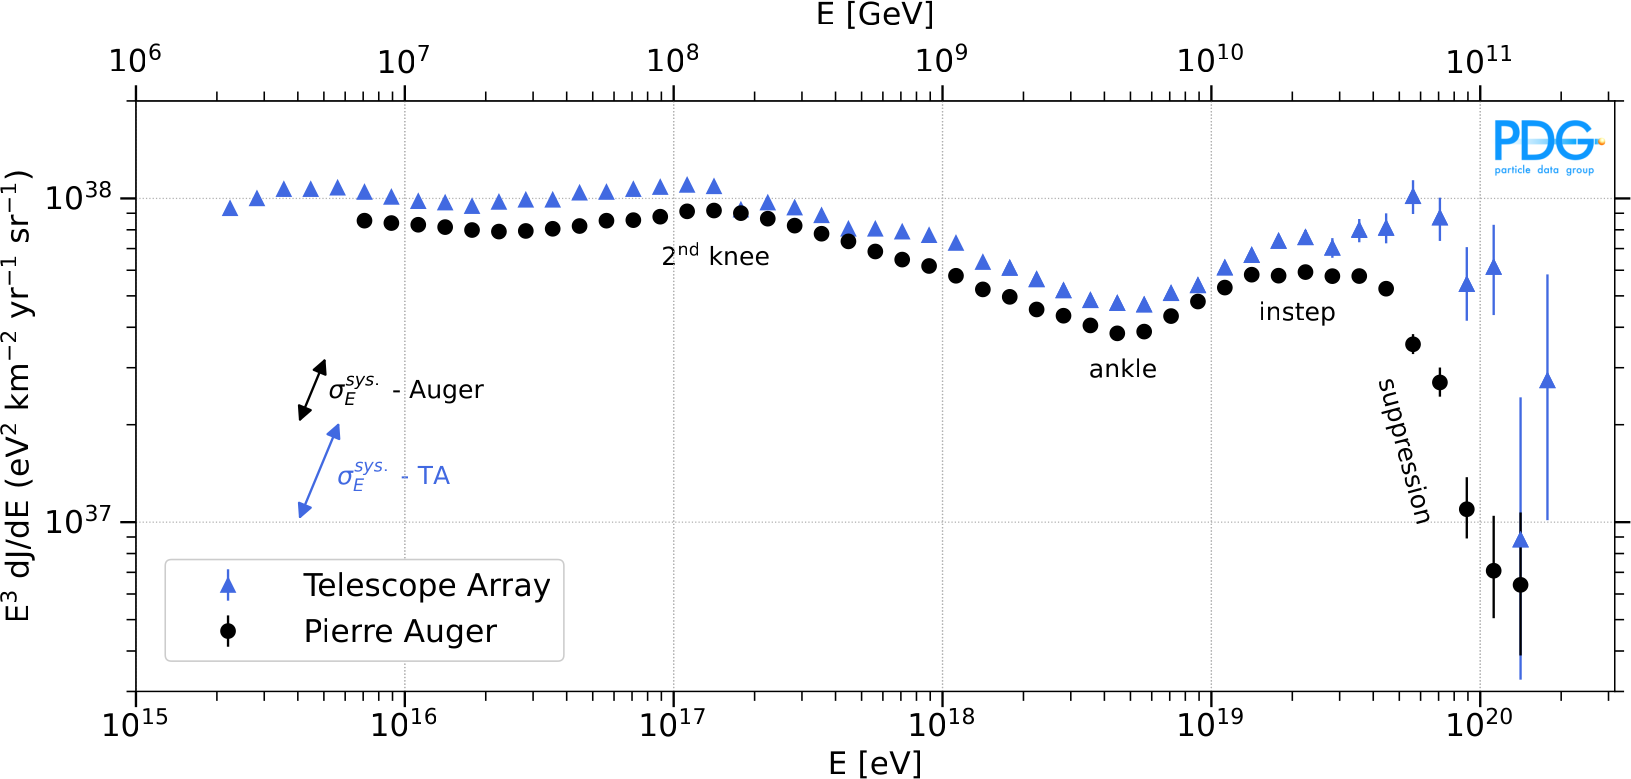
\includegraphics[width=\linewidth]{tesis/espectro_uhecr_recortado.png}
    \column{0.37\textwidth}
      \small
      Auger (2020), ley de potencia quebrada:\\[4pt]
      {\footnotesize
      \begin{tabular}{@{}lr@{}}
        \toprule
        tobillo & $E_{12}=5{,}0$\,EeV \\
        \emph{instep} & $E_{23}=13$\,EeV \\
        supresión & $E_{34}=46$\,EeV \\
        \midrule
        $\gamma_1\to\gamma_2$ & $3{,}29\to2{,}51$\\
        $\gamma_3\to\gamma_4$ & $3{,}05\to5{,}1$\\
        \bottomrule
      \end{tabular}}\\[6pt]
      \begin{clave}
        Supresión a más de 20$\sigma$. ¿Propagación o límite de las fuentes?
        El espectro solo no alcanza.
      \end{clave}
  \end{columns}
  \credito{Figura: PDG (2024), datos de Pierre Auger y Telescope Array}
\end{frame}

% ---------------------------------------------------------------- 19
\begin{frame}{Cómo se acelera: el mecanismo de Fermi en choques}
  \begin{columns}[c,onlytextwidth]
    \column{0.46\textwidth}
      \centering
      \begin{tikzpicture}[x=1cm,y=1cm]
        \fill[itedaOrange!10] (-3,-1.6) rectangle (0,1.9);
        \fill[cmbAzul!10] (0,-1.6) rectangle (3,1.9);
        \draw[itedaOrange, line width=2pt] (0,-1.6) -- (0,1.9);
        \node[font=\scriptsize, align=center] at (-1.5,1.55) {gas ya chocado};
        \node[font=\scriptsize, align=center] at (1.5,1.55) {gas en reposo};
        \draw[flecha, itedaOrange] (-0.6,-1.25) -- (0.6,-1.25)
          node[right, font=\tiny, text=itedaTealDark] {el choque avanza};
        \draw[very thick, violetaNu, -{Stealth}, rounded corners=4pt]
          (-2.3,-0.4) -- (-1.2,0.2) -- (-0.4,-0.3) -- (0.9,0.5) -- (2.2,0.1)
          -- (1.2,0.9) -- (-0.7,0.6) -- (-1.6,1.0) -- (-0.3,0.95) -- (1.7,0.75);
        \foreach \x/\y in {-2.2/0.7,-1.4/-0.8,-0.6/1.2,0.8/-0.6,1.6/1.1,2.4/-0.3}{
          \draw[itedaGray!70, decorate, decoration={coil, aspect=0.4, segment length=1.6mm, amplitude=0.9mm}]
            (\x-0.25,\y) -- (\x+0.25,\y);}
        \node[font=\scriptsize, text=violetaNu] at (2.35,0.95) {$E\uparrow$};
      \end{tikzpicture}\\[4pt]
      {\scriptsize Espirales grises: irregularidades del campo magnético que
      actúan como «espejos».}
    \column{0.51\textwidth}
      \footnotesize
      \begin{enumerate}\footnotesize
        \item Una supernova lanza una \textbf{onda de choque} a miles de km/s.
        \item Campos magnéticos \textbf{turbulentos} a ambos lados hacen
          rebotar a la partícula, que cruza el choque una y otra vez.
        \item En cada cruce el gas del otro lado \textbf{viene hacia ella},
          como una pelota entre dos raquetas que se acercan: gana $\sim$1\% de
          energía.
        \item En cada vuelta puede \textbf{escaparse} y dejar de acelerarse.
      \end{enumerate}
      \begin{clave}
        Muchas ganan poco y pocas muchísimo: una \textbf{ley de potencia}
        $E^{-2}$ ($E^{-2,7}$ tras escapar de la galaxia).
      \end{clave}
  \end{columns}
\end{frame}

% ---------------------------------------------------------------- 20
\begin{frame}{Criterio de Hillas: ¿quién llega a $10^{20}$ eV?}
  \begin{columns}[c,onlytextwidth]
    \column{0.52\textwidth}
      \centering
      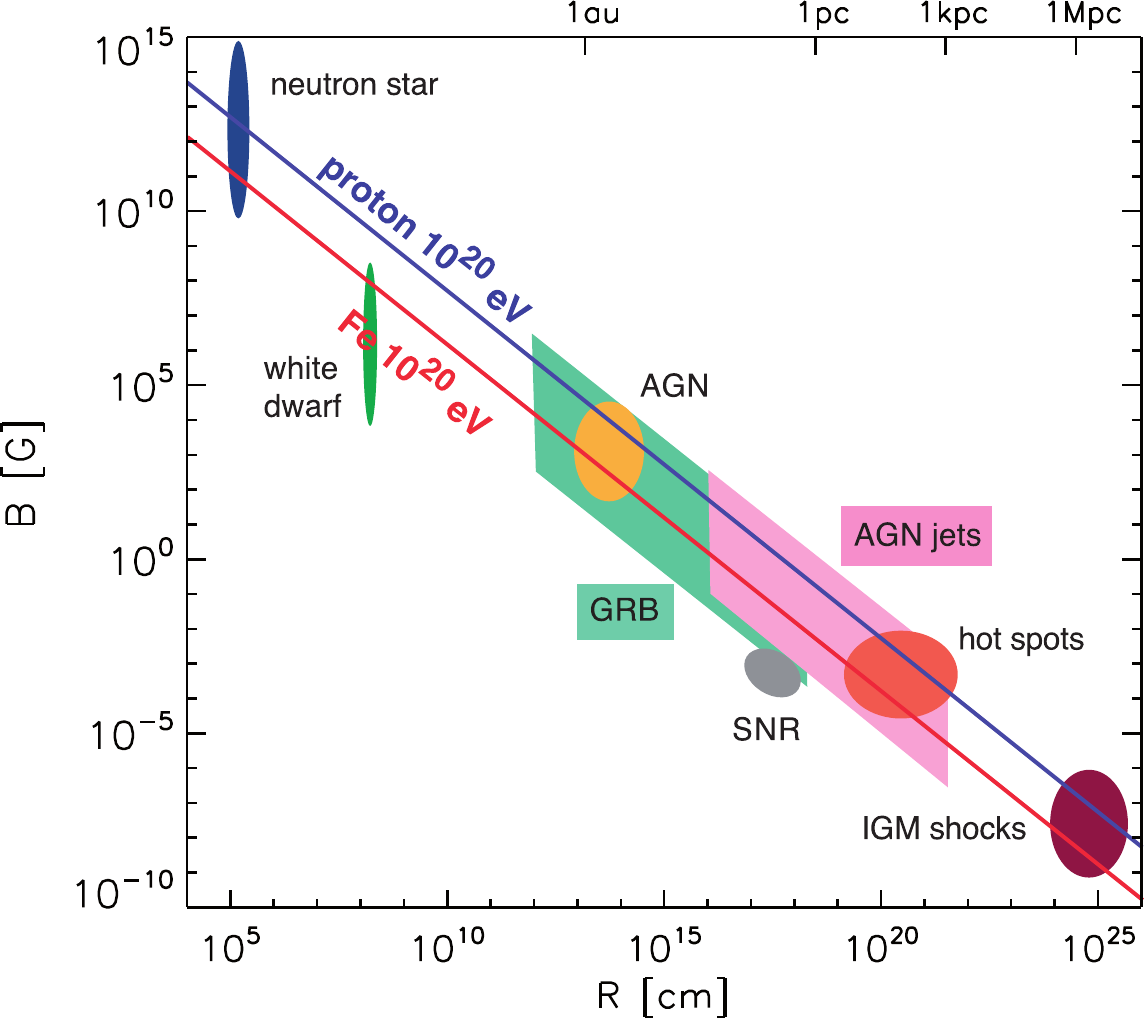
\includegraphics[width=\linewidth]{externas/hillas_aloisio2017.png}
    \column{0.45\textwidth}
      \small
      Para seguir ganando energía, la partícula tiene que quedar
      \textbf{atrapada} girando en la región que la acelera: su radio de giro
      debe ser menor que el tamaño de la fuente.
      \vspace{2pt}
      \begin{clave}
        \centering
        $E_\mathrm{max}\;\approx\;Z\;\beta\;B\;R$
      \end{clave}
      \vspace{2pt}
      {\footnotesize $Z$: carga del núcleo (el hierro llega 26 veces más
      lejos) · $\beta$: velocidad del choque · $B$: campo magnético · $R$:
      tamaño.}\\[4pt]
      {\footnotesize Sobre las diagonales se llega a $10^{20}$\,eV: campos
      enormes en objetos chicos o débiles en regiones gigantes. Necesario, no
      suficiente.}
  \end{columns}
  \creditoizq{Figura: Kotera \& Olinto, ARA\&A 49 (2011) 119, vía Aloisio, PTEP 2017 12A102 (Fig.~12)}
\end{frame}

% ---------------------------------------------------------------- 22
\begin{frame}{El viaje no es gratis: efecto GZK y fotodesintegración}
  \begin{columns}[c,onlytextwidth]
    \column{0.52\textwidth}
      \centering
      \begin{tikzpicture}[x=1cm,y=1cm]
        \node[font=\small\bfseries] (p) at (0,0) {$p$};
        \node[font=\small, text=cmbAzul] (g) at (0,-1.4) {$\gamma_\mathrm{CMB}$};
        \node[circle, fill=itedaOrange!25, draw=itedaOrange, font=\small, inner sep=1pt]
          (D) at (1.6,-0.7) {$\Delta^+$};
        \draw[flecha] (p) -- (D);
        \draw[foton, cmbAzul] (g) -- (D);
        \node[font=\small, anchor=west] (n) at (2.8,0.2) {$n\,\pi^+$};
        \node[font=\small, anchor=west] (pp) at (2.8,-1.6) {$p\,\pi^0$};
        \draw[flecha] (D) -- (n.west);
        \draw[flecha] (D) -- (pp.west);
        \node[font=\small, text=violetaNu, anchor=west] at (3.6,0.2)
          {$\to\mu^+\nu_\mu\to e^+\nu_e\bar\nu_\mu\nu_\mu$};
        \node[font=\small, text=cmbAzul, anchor=west] at (3.6,-1.6) {$\to\gamma\gamma$};
        \node[font=\scriptsize, text=violetaNu, anchor=north] at (5.0,-0.1)
          {neutrinos \textbf{cosmogénicos}};
      \end{tikzpicture}\\[6pt]
      \small
      \[ E_\mathrm{th}=\frac{m_\pi\,(2m_p+m_\pi)}{4\varepsilon}\approx10^{20}\,\mathrm{eV}
         \quad (\varepsilon\approx6\times10^{-4}\,\mathrm{eV}) \]
      {\footnotesize La cola de Planck lo baja a $\sim5\times10^{19}$\,eV.
      Pierde $\sim$20\% por interacción: horizonte de $\sim$50--100\,Mpc.}
    \column{0.45\textwidth}
      \small
      \begin{itemize}\footnotesize
        \item \textbf{Protones}: piones (GZK, 1966) y pares $e^+e^-$.
        \item \textbf{Núcleos}: fotodesintegración en el CMB y el fondo
          infrarrojo; umbral $\propto A$.
        \item \textbf{Fuentes}: energía máxima $E_\mathrm{max}\propto Z$.
      \end{itemize}
      \begin{clave}
        Los escenarios \textbf{no se excluyen}. Separarlos requiere
        \textbf{espectro, composición y anisotropías}.
      \end{clave}
  \end{columns}
\end{frame}

% ---------------------------------------------------------------- 23
\begin{frame}{Composición y direcciones de llegada}
  \begin{columns}[T,onlytextwidth]
    \column{0.50\textwidth}
      \centering
      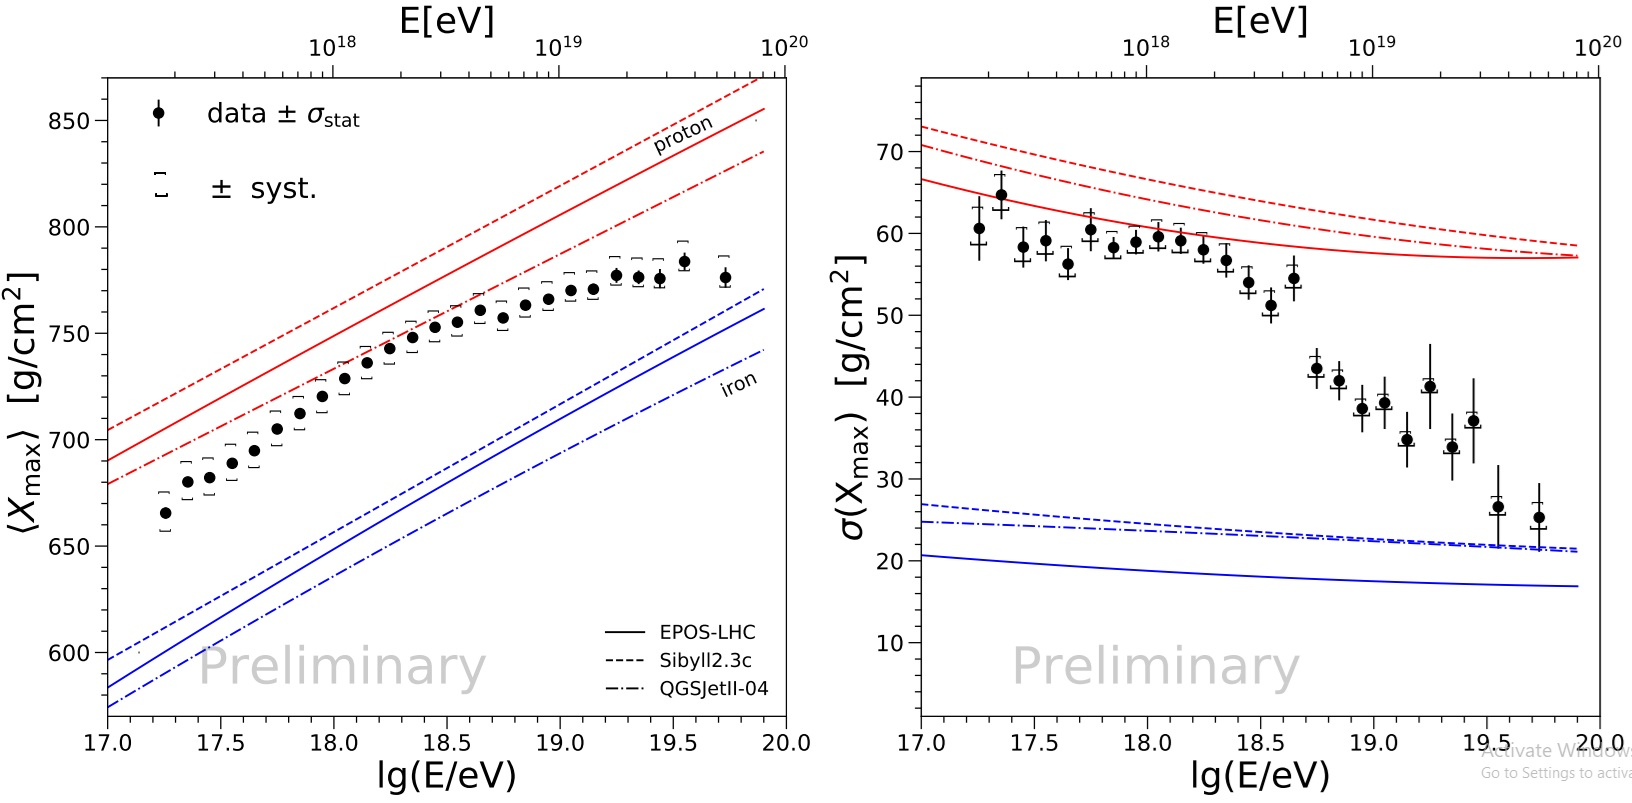
\includegraphics[width=\linewidth]{tesis/x_max.jpg}\\[3pt]
      {\footnotesize $\langle X_\mathrm{max}\rangle$ y $\sigma(X_\mathrm{max})$ se
      alejan de protón: composición \textbf{más pesada} por encima de
      $\sim$3\,EeV.}
    \column{0.47\textwidth}
      \centering
      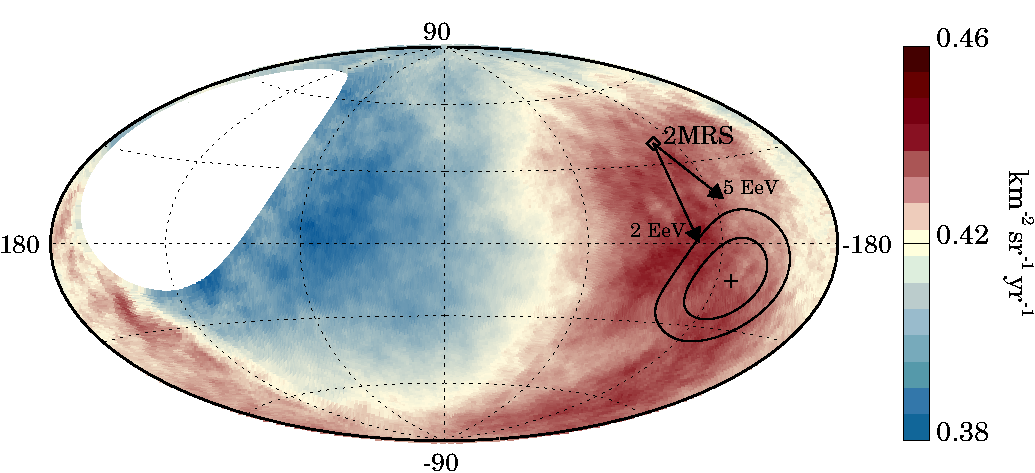
\includegraphics[width=0.9\linewidth]{externas/auger_dipolo_galactico_2017.pdf}\\[2pt]
      {\footnotesize Por encima de 8\,EeV: un \textbf{dipolo} de $\sim$7\% lejos
      del centro galáctico ($>6\sigma$): \textbf{origen extragaláctico}.}\\[4pt]
      \begin{clave}
        Favorece fuentes de \textbf{rigidez máxima limitada} y composición
        mixta (según el modelo hadrónico).
      \end{clave}
  \end{columns}
  \creditoizq{Izq.: Auger (A.~Yushkov), ICRC 2019. Der.: Auger, Science 357 (2017) 1266; significancia: ICRC 2025}
\end{frame}

% ======================================================================
% BLOQUE 3 — El Observatorio Pierre Auger
% ======================================================================
\section{Observatorio Pierre Auger}
\bloque{PIERRE AUGER}

% ---------------------------------------------------------------- 24
\begin{frame}[plain]
  \fondo[0.05]{externas/auger_tanque_escala.jpg}
  \velo[0.85]{l}
  \begin{tikzpicture}[remember picture, overlay]
    \node[anchor=north west, text=white, align=left, text width=6.2cm]
      at ([xshift=0.7cm, yshift=-0.8cm]current page.north west) {%
      {\Large\bfseries ¿Cómo se mide algo que llega una vez por km$^2$ por siglo?}\\[4pt]
      {\footnotesize (por encima de $\sim5\times10^{19}$\,eV)}\\[8pt]
      {\large $N = J\cdot A\cdot\Omega\cdot T$}\\[10pt]
      {\small Con $A\approx3000$\,km$^2$ ---unas 15 veces la Ciudad de
      Buenos Aires---, funcionando día y noche desde 2004.}\\[6pt]
      {\small Resultado: $\approx$50.000 eventos por encima de 8\,EeV en 19 años.}};
    \node[anchor=south west, text=white!85, font=\scriptsize, text width=6cm]
      at ([xshift=0.7cm, yshift=0.45cm]current page.south west)
      {Una estación del detector de superficie en la Pampa Amarilla, Malargüe};
  \end{tikzpicture}
  \creditoblanco{Foto: T.~Schulz, CC BY-SA 4.0 (Wikimedia Commons) \quad Estadística: Auger, ICRC 2025}
\end{frame}

% ---------------------------------------------------------------- 25
\begin{frame}{Una partícula con la energía de una pelota de béisbol}
  \begin{columns}[c,onlytextwidth]
    \column{0.57\textwidth}
      \centering
      \begin{tikzpicture}[x=0.56cm, y=0.8cm]
        \draw[itedaGray, thick, -{Stealth}] (9,0) -- (21.4,0);
        \node[font=\scriptsize, text=itedaGray, anchor=north] at (15,-0.4) {energía [eV]};
        \foreach \x in {9,11,...,21}{\draw[itedaGray] (\x,-0.08) -- (\x,0.08)
          node[below=3pt, font=\tiny, text=itedaGray] {$10^{\x}$};}
        \tikzset{marca/.style={thick, -{Stealth}}}
        \draw[marca, itedaTeal, very thick] (12.83,1.5) -- (12.83,0.12);
        \node[font=\small\bfseries, text=itedaTeal, align=center, anchor=south] at (12.83,1.5)
          {protón del LHC\\6,8\,TeV};
        \draw[marca, itedaOrange, very thick] (20,1.5) -- (20,0.12);
        \node[font=\small\bfseries, text=itedaOrange, align=center, anchor=south] at (20,1.5)
          {rayo cósmico\\$10^{20}$\,eV};
        \draw[decorate, decoration={brace, amplitude=6pt, mirror}, thick, itedaTealDark]
          (12.83,-0.95) -- (20,-0.95);
        \node[font=\small\bfseries, text=itedaTealDark, anchor=north] at (16.4,-1.15)
          {$\times\,10^{7}$: siete órdenes de magnitud};
      \end{tikzpicture}\\[4pt]
      \begin{minipage}[c]{0.3\linewidth}
        \centering
        \begin{tikzpicture}[scale=0.68]
          \fill[noche, rounded corners=3pt] (-1.75,-1.75) rectangle (1.75,1.75);
          \draw[white!70, thin] (0,0) circle (1.45);
          \fill[white!80] (1.45,0) circle (1.5pt);
          \node[font=\tiny, text=white!80] at (0,1.25) {Mercurio};
          \draw[itedaOrange, very thick, dashed] (0,0) circle (1.0);
          \shade[ball color=yellow!80!orange] (0,0) circle (0.14);
          \node[font=\tiny\bfseries, text=itedaOrange] at (0,-0.55) {«LHC»};
        \end{tikzpicture}
      \end{minipage}\hfill
      \begin{minipage}[c]{0.67\linewidth}
        \footnotesize\raggedright
        ¿Un LHC para $10^{20}$\,eV? Con los mismos imanes (8\,T), su radio
        sería de \textbf{$\sim$40 millones de km}: casi la \textbf{órbita de
        Mercurio}.
      \end{minipage}
    \column{0.40\textwidth}
      \begin{clave}
        \large
        $10^{20}$\,eV $\approx$ \textbf{16\,J}\\[6pt]
        \normalsize
        Una pelota de béisbol (145\,g) a 90\,km/h tiene \textbf{45\,J}.\\[6pt]
        El récord, Fly's Eye (1991): $3{,}2\times10^{20}$\,eV $\approx$
        \textbf{51\,J}.\\[6pt]
        La energía de una pelota rápida, \textbf{en un solo núcleo}.
      \end{clave}
      \vspace{4pt}
      {\scriptsize\color{itedaGray} En el centro de masa, el choque con un
      núcleo del aire equivale a «sólo» $\sim$30 LHC.}
  \end{columns}
\end{frame}

% ---------------------------------------------------------------- 26
\begin{frame}{El Observatorio Pierre Auger, en Malargüe}
  \begin{columns}[c,onlytextwidth]
    \column{0.40\textwidth}
      \centering
      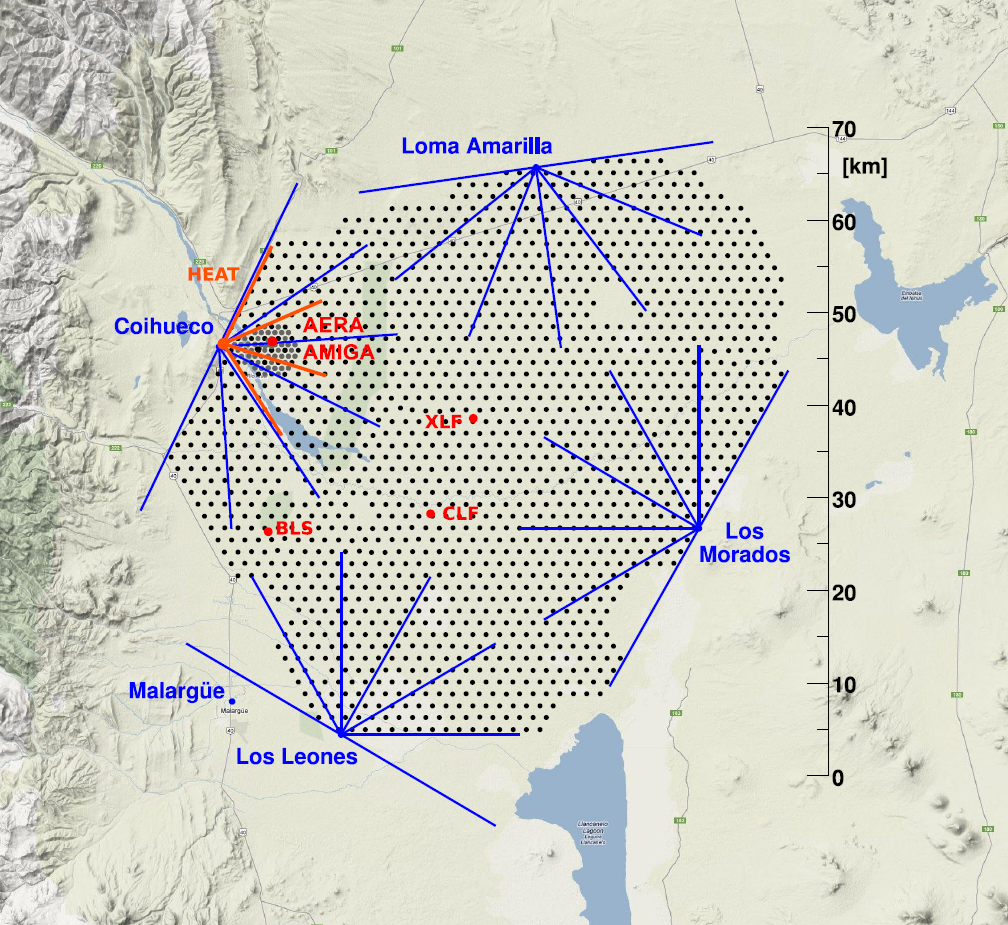
\includegraphics[width=0.98\linewidth]{tesis/mapa_auger.png}
    \column{0.57\textwidth}
      \small
      \begin{itemize}\footnotesize
        \item Propuesto por J.~Cronin y A.~Watson (1991--92) para resolver la
          controversia sobre la supresión.
        \item Construcción 2002--2008; datos desde 2004.
        \item \textbf{1660 tanques} cada 1500\,m ($\approx$3000\,km$^2$) y
          \textbf{27 telescopios} de fluorescencia en 4 sitios.
        \item Arreglos densos (750 y 433\,m) para energías menores: allí está
          \textbf{AMIGA}.
        \item $\sim$400 científicos de 17 países.
      \end{itemize}
      \vspace{3pt}
      \begin{clave}
        Argentina es el país sede. Grupos argentinos ---entre ellos ITeDA---
        diseñan, construyen y operan detectores y analizan los datos.
      \end{clave}
  \end{columns}
  \credito{Mapa: Botti (2019)}
\end{frame}

% ---------------------------------------------------------------- 27
\begin{frame}{Lluvias atmosféricas extensas}
  \begin{columns}[c,onlytextwidth]
    \column{0.42\textwidth}
      \centering
      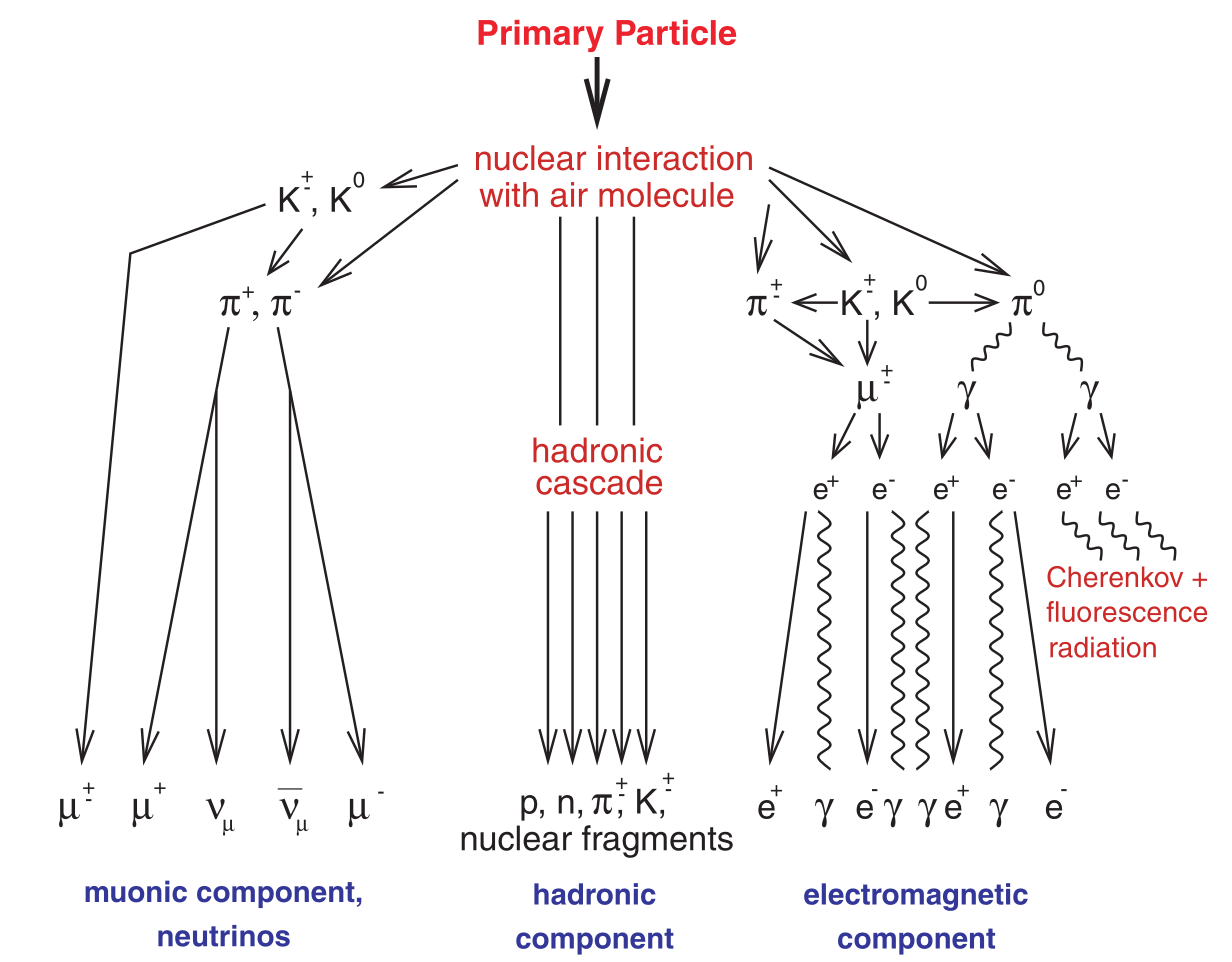
\includegraphics[height=4.1cm]{tesis/eas.png}\\[2pt]
      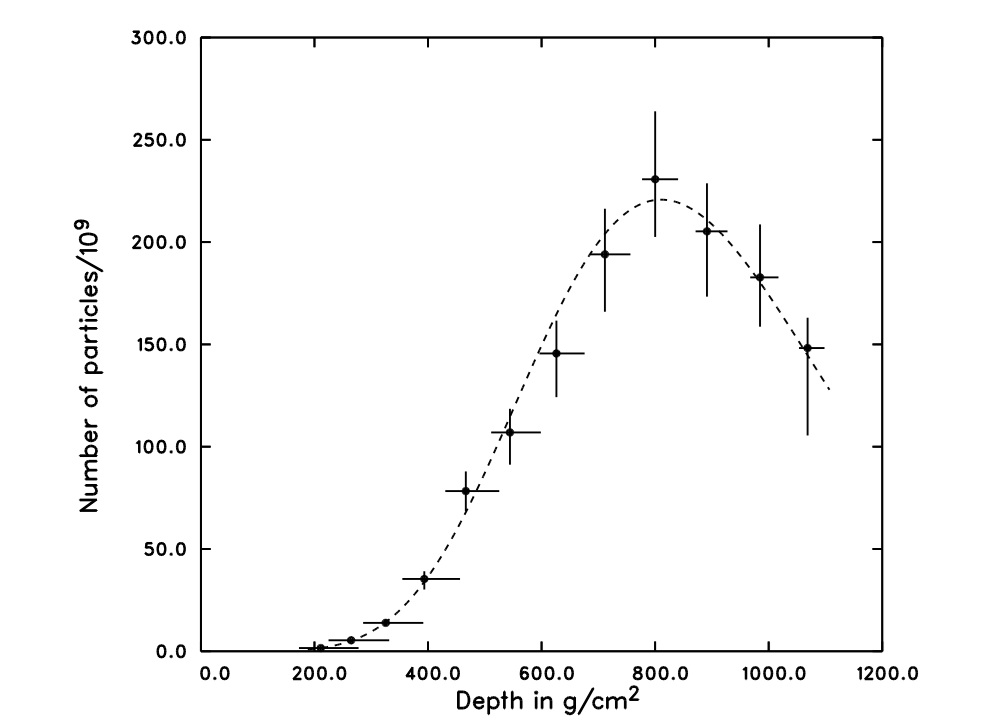
\includegraphics[height=1.9cm]{tesis/ammount_xmax.jpg}\\
      {\tiny Perfil del evento de Fly's Eye ($3{,}2\times10^{20}$\,eV)}
    \column{0.55\textwidth}
      \small
      Primera interacción a $\sim$15--20\,km de altura:
      \begin{itemize}\footnotesize
        \item $\pi^0\to\gamma\gamma$: componente \textbf{electromagnética},
          $\sim$90\% de la energía.
        \item $\pi^\pm\to\mu^\pm\nu_\mu$: componente \textbf{muónica}, penetrante.
      \end{itemize}
      Heitler--Matthews: un núcleo $A$ son $A$ nucleones de energía $E/A$.
      \[ \langle X_\mathrm{max}\rangle \simeq X_0^p + D_{10}\log_{10}\frac{E}{A},
         \quad N_\mu \simeq A\left(\frac{E/A}{\xi_c^\pi}\right)^{\!\beta} \]
      \begin{clave}
        Con $\beta\approx0{,}9$: el hierro tiene $\sim$1,5 veces más muones y llega
        a su máximo $\sim$100\,g/cm$^2$ antes que un protón.
      \end{clave}
  \end{columns}
  \credito{Esquema: Haungs \textit{et al.} (2003). Perfil: Bird \textit{et al.}, ApJ 441 (1995) 144}
\end{frame}

% ---------------------------------------------------------------- 28
\begin{frame}{Detección híbrida: el suelo y el cielo}
  \begin{columns}[T,onlytextwidth]
    \column{0.31\textwidth}
      \centering
      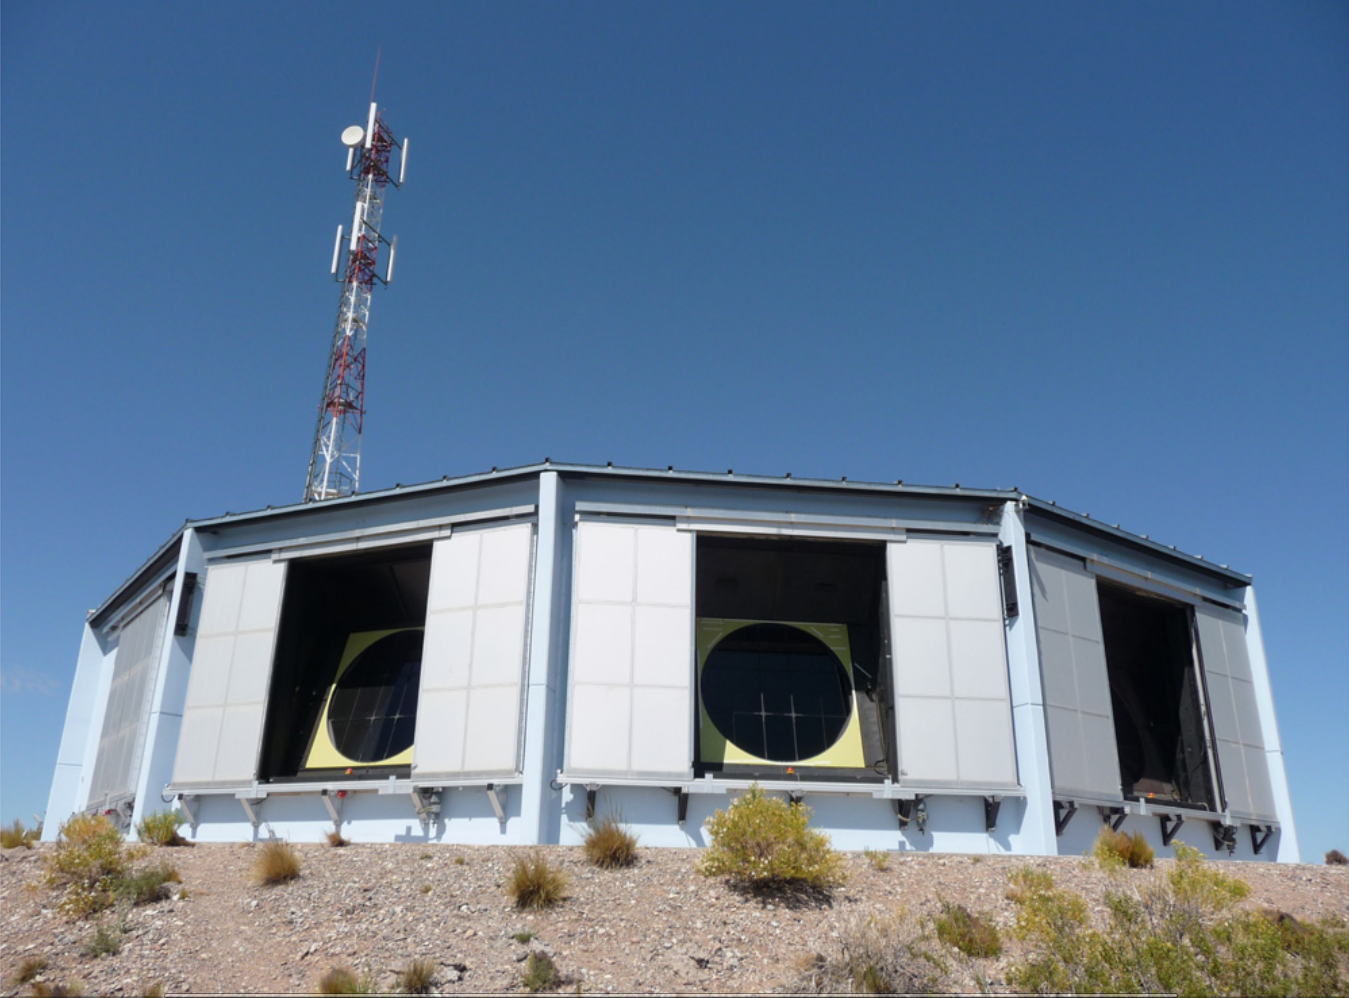
\includegraphics[width=\linewidth]{tesis/fd_leones.png}\\[2pt]
      {\small\bfseries Fluorescencia (FD)}\\[1pt]
      {\footnotesize El N$_2$ excitado emite UV: se \textbf{ve la lluvia
      crecer}. Sólo en noches oscuras ($\sim$15\%).}
    \column{0.31\textwidth}
      \centering
      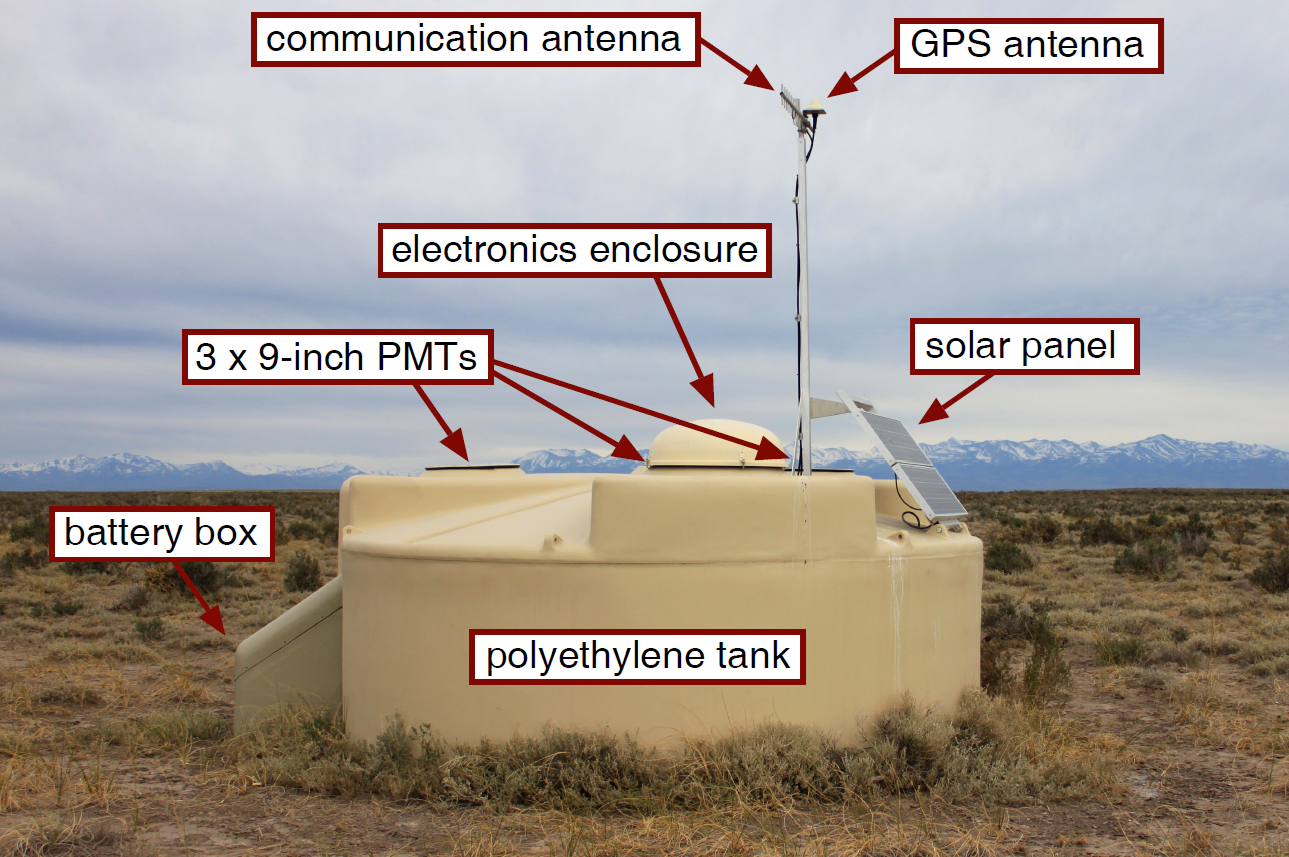
\includegraphics[width=\linewidth]{tesis/ssd.png}\\[2pt]
      {\small\bfseries Superficie (SD)}\\[1pt]
      {\footnotesize 12.000\,l de agua ultrapura y 3 PMT muestrean las
      partículas en el suelo, \textbf{día y noche}.}
    \column{0.33\textwidth}
      \centering
      \begin{tikzpicture}[x=1cm,y=1cm]
        \tikzset{caja/.style={rounded corners=2pt, inner sep=3pt,
          font=\footnotesize, text width=4.1cm, align=left}}
        \node[caja, fill=itedaOrange!15] (a) at (0,2.1)
          {\textbf{FD}: perfil $dE/dX$ $\to$ energía y $X_\mathrm{max}$};
        \node[caja, fill=itedaTeal!15] (b) at (0,0.7)
          {\textbf{SD}: densidad lateral $\to$ $S(1000)$ y dirección};
        \draw[flecha, itedaTealDark] (a.south) -- (b.north)
          node[midway, right, font=\tiny] {calibra};
      \end{tikzpicture}\\[6pt]
      \begin{clave}
        Los eventos \textbf{híbridos} calibran la energía del SD sin
        depender de simulaciones: escala con $\sim$14\% de sistemático.
      \end{clave}
  \end{columns}
  \credito{Fotos: Colaboración Pierre Auger, NIM A 798 (2015); Botti (2019)}
\end{frame}

% ---------------------------------------------------------------- 29
\begin{frame}{AugerPrime y AMIGA: separar electrones de muones}
  \begin{columns}[c,onlytextwidth]
    \column{0.35\textwidth}
      \centering
      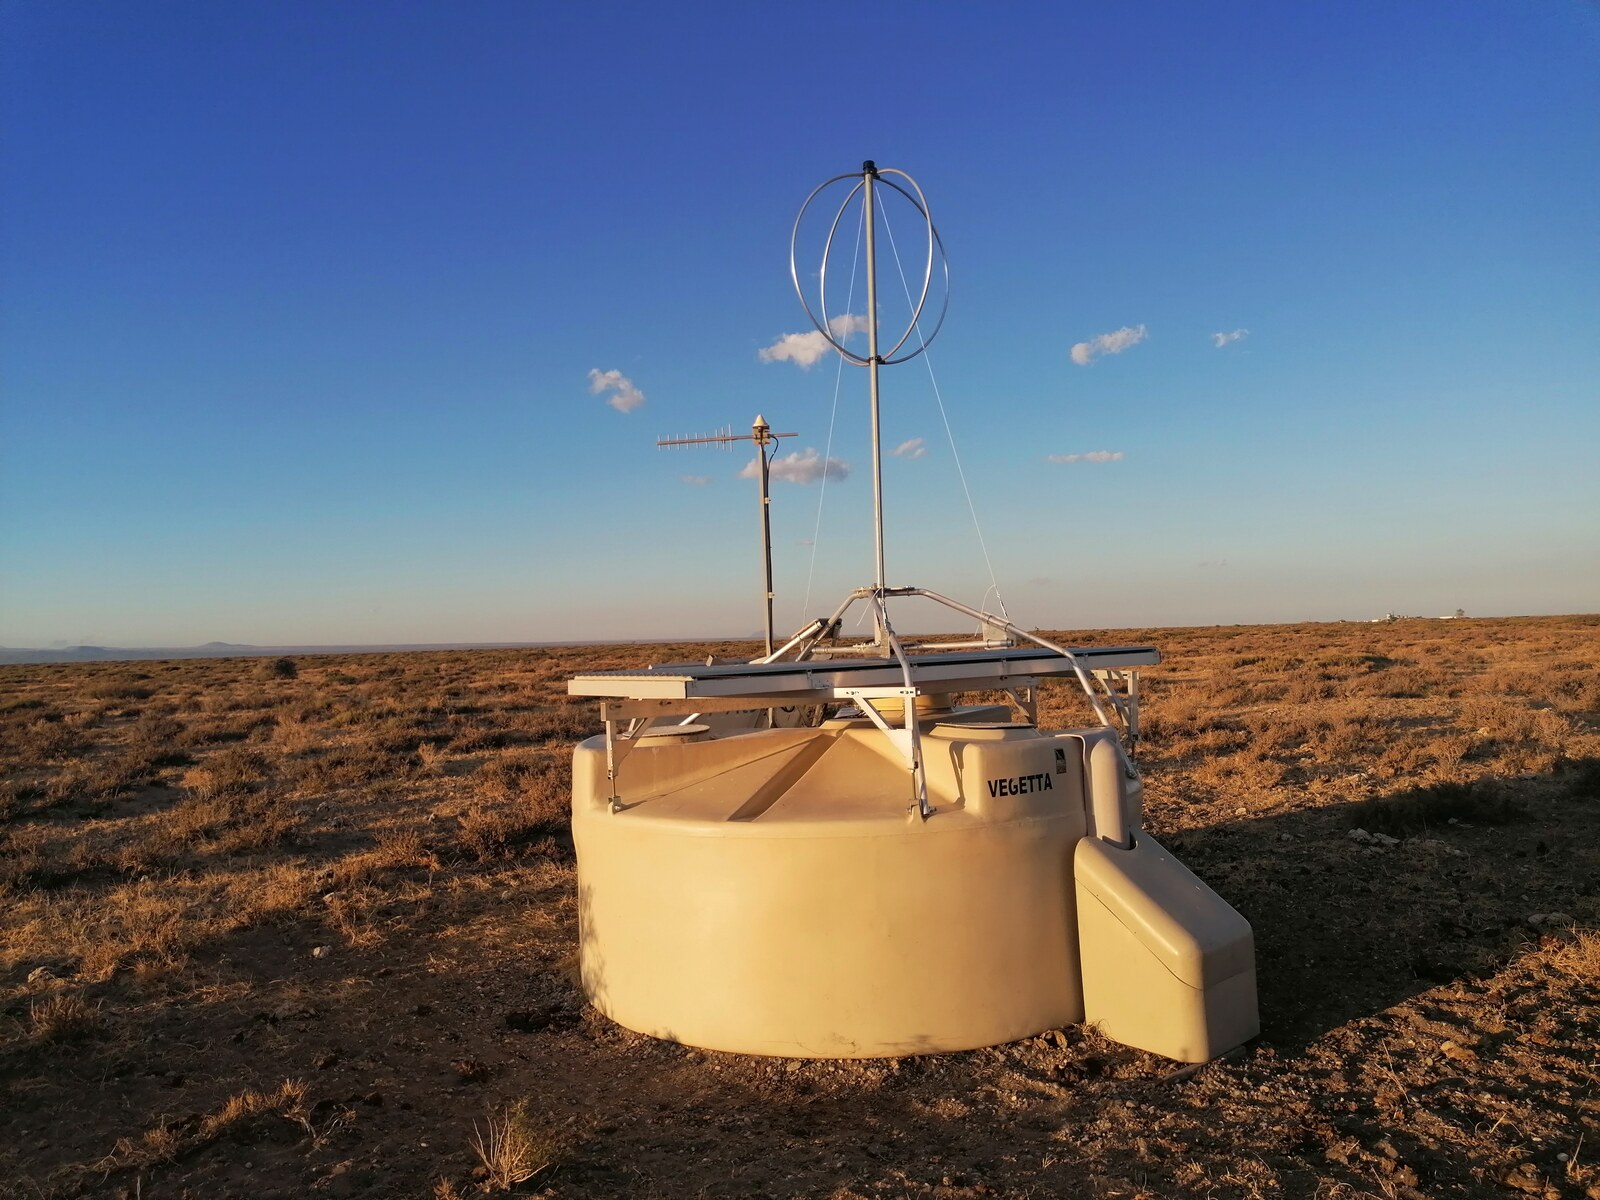
\includegraphics[width=\linewidth]{tesis/estacion_augerprime.jpg}\\[1pt]
      {\scriptsize Estación de AugerPrime}
    \column{0.30\textwidth}
      \begin{itemize}\footnotesize
        \item \textbf{SSD}: centellador de 3,8\,m$^2$ sobre el tanque.
        \item \textbf{RD}: antena de radio, 30--80\,MHz.
        \item \textbf{UMD}: muones \textbf{bajo tierra}.
      \end{itemize}
    \column{0.31\textwidth}
      \centering
      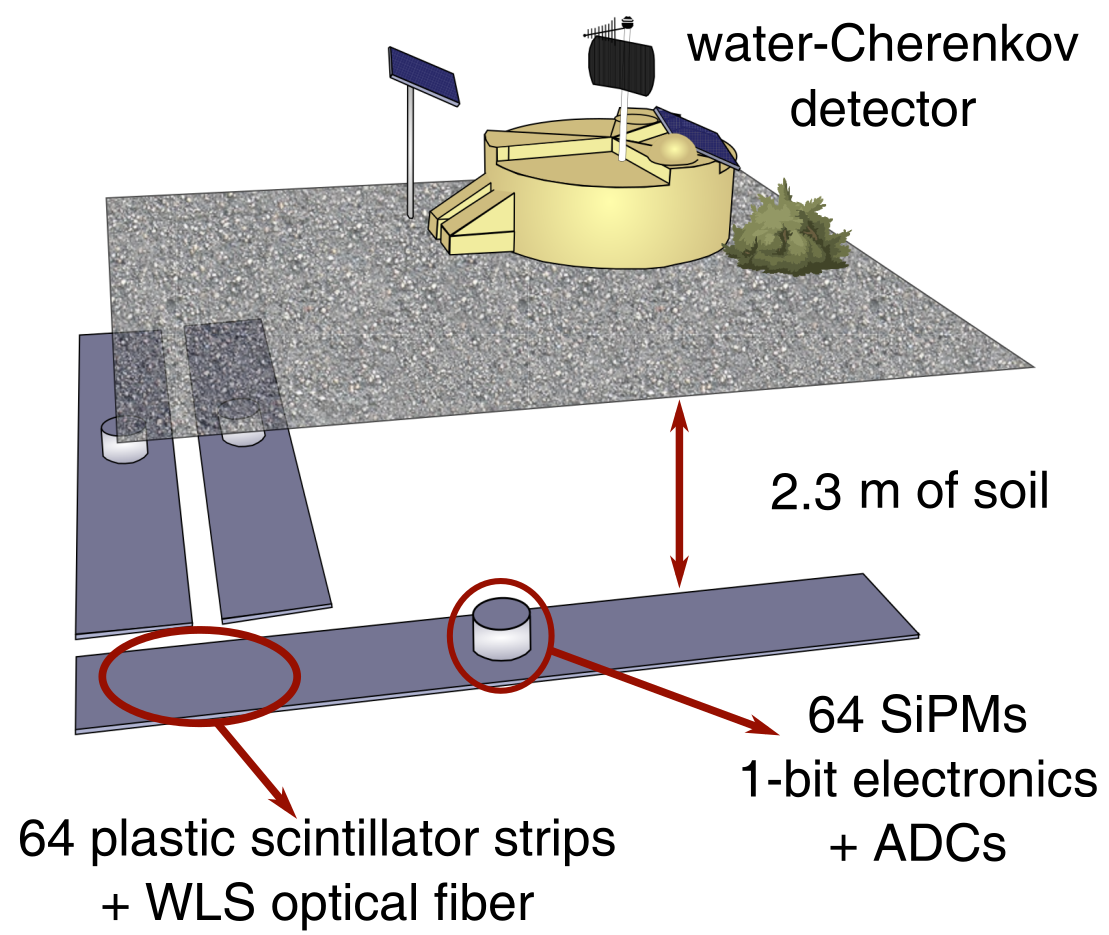
\includegraphics[width=\linewidth]{tesis/umd.png}\\[1pt]
      {\scriptsize AMIGA: módulos enterrados junto a los tanques}
  \end{columns}
  \vspace{8pt}
  \begin{clave}
    Tanque + centellador separan las componentes \textbf{estadísticamente};
    el UMD las separa \textbf{físicamente}: la tierra absorbe lo electromagnético.
  \end{clave}
  \credito{Foto: Colaboración Pierre Auger. Esquema: Botti (2019)}
\end{frame}

% ---------------------------------------------------------------- 30
\begin{frame}{El efecto Cherenkov: una onda de choque de luz}
  \begin{columns}[T,onlytextwidth]
    \column{0.30\textwidth}
      \centering
      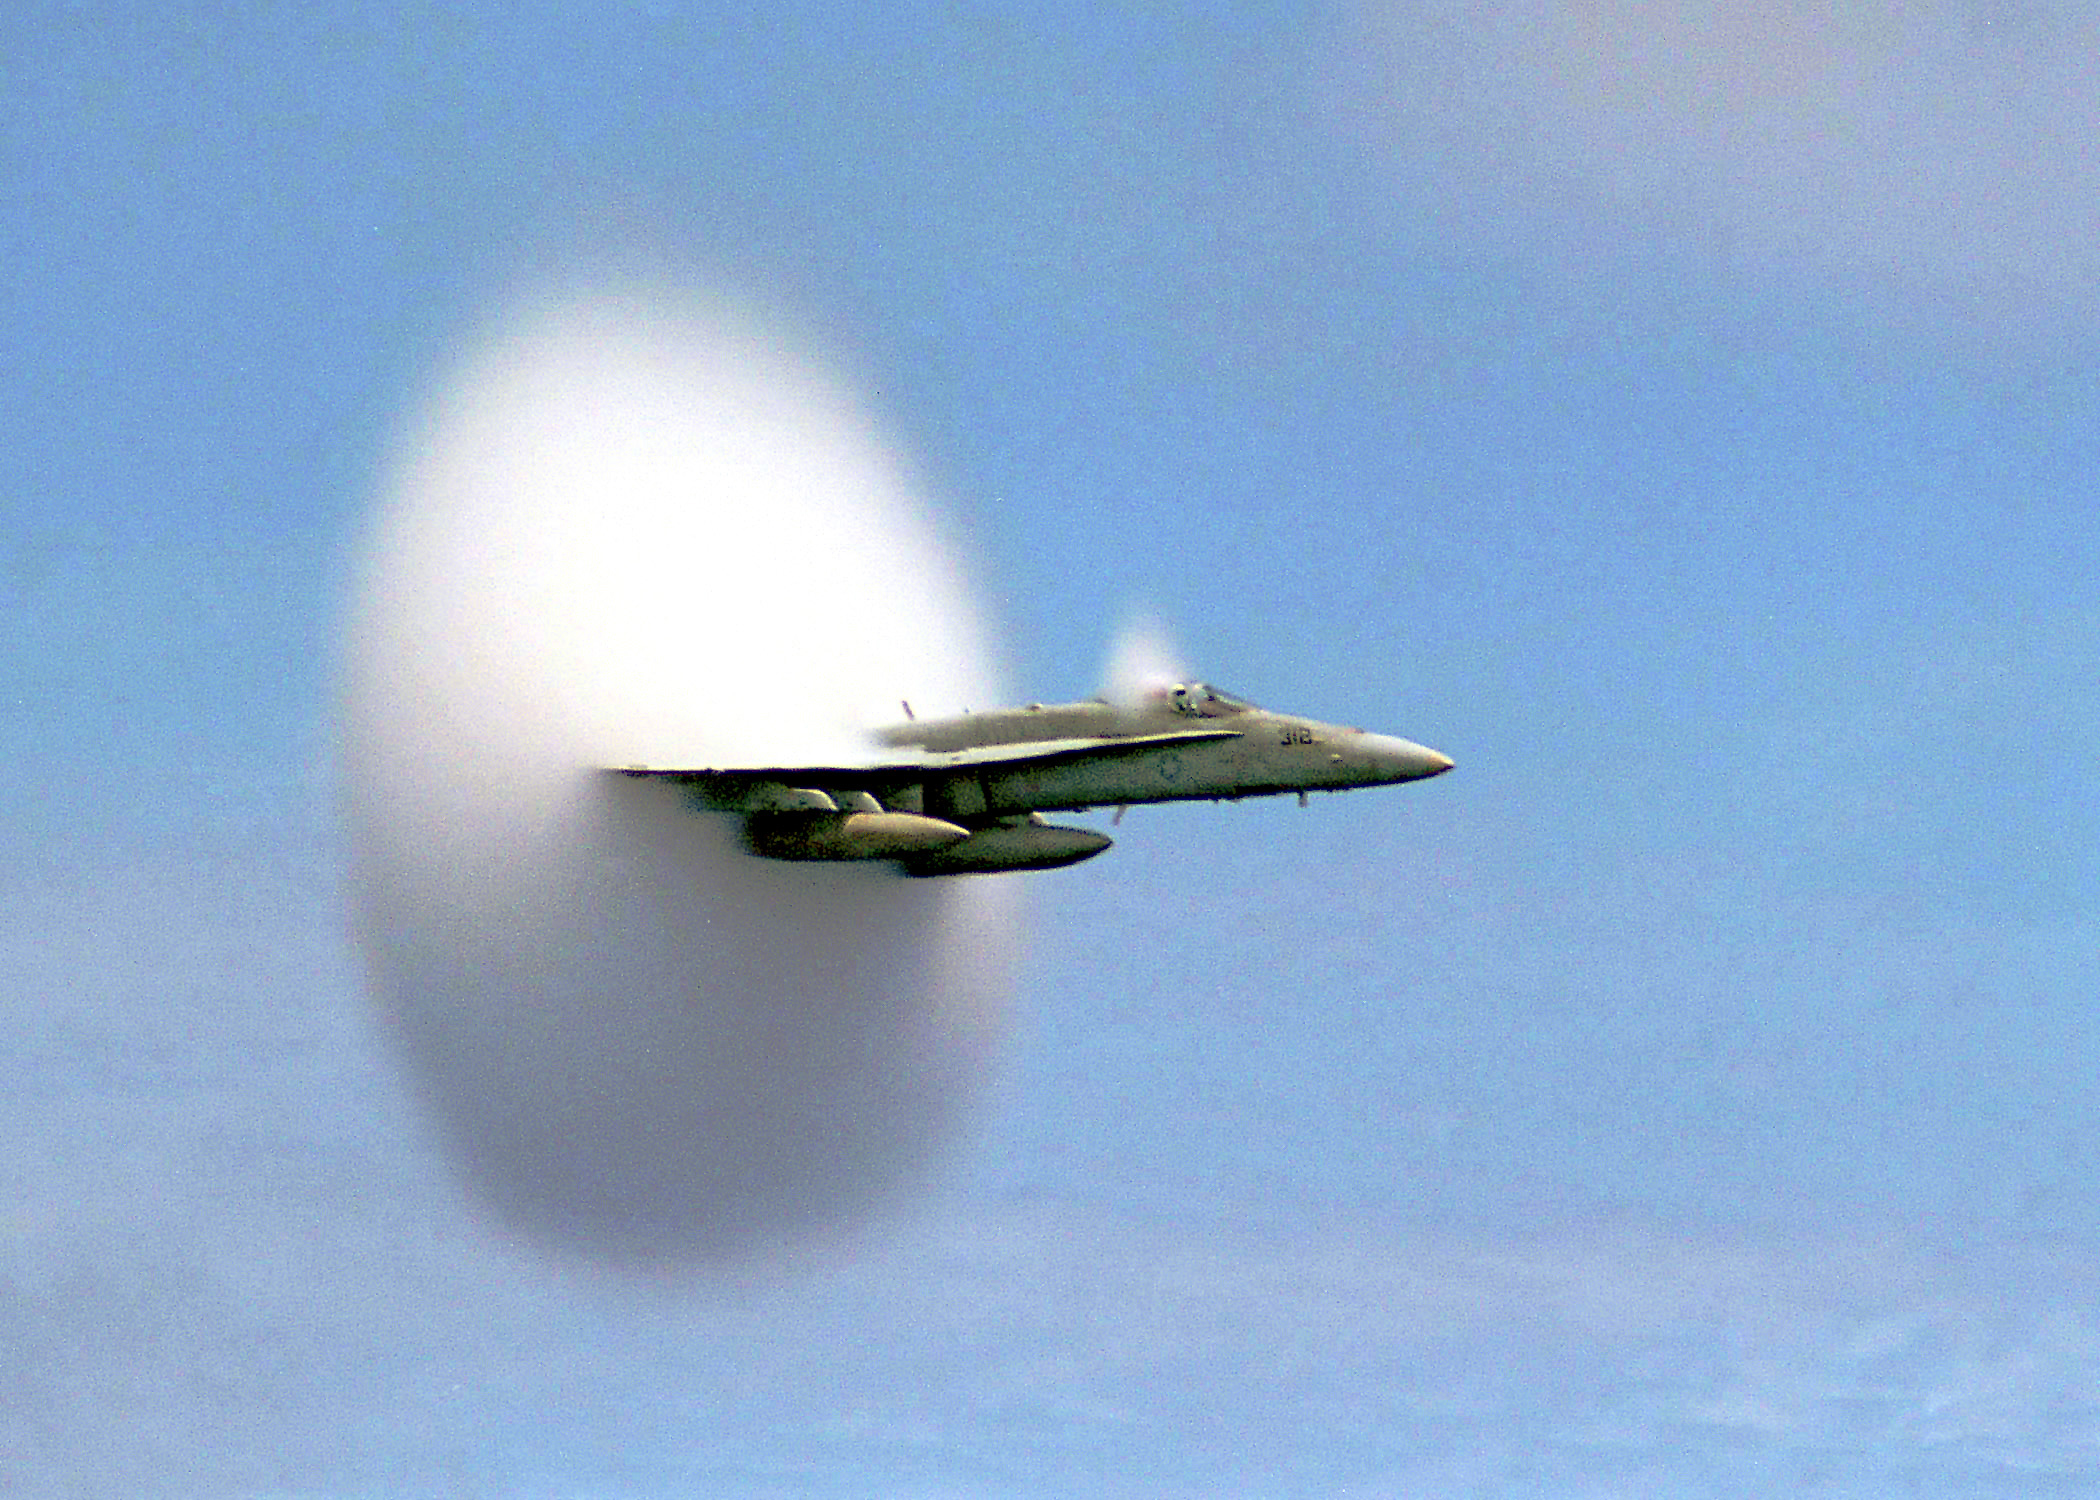
\includegraphics[width=\linewidth]{externas/fa18_cono_vapor.jpg}\\[3pt]
      \begin{tikzpicture}[x=0.42cm,y=0.42cm]
        \begin{scope}
          \clip (-4.6,-2.3) rectangle (1.6,2.3);
          \foreach \i in {0,...,4}{
            \pgfmathsetmacro{\xx}{-4+\i}\pgfmathsetmacro{\rr}{0.6*(5-\i)}
            \draw[itedaGray] (\xx,0) circle (\rr);}
          \draw[itedaOrange, thick] (1,0) -- ++(143.1:4.2);
          \draw[itedaOrange, thick] (1,0) -- ++(216.9:4.2);
        \end{scope}
        \fill[itedaTealDark] (1,0) circle (2.2pt);
      \end{tikzpicture}\\[1pt]
      {\footnotesize Sonido: $\sin\alpha = v_s/v$}
    \column{0.36\textwidth}
      \centering
      \begin{tikzpicture}[x=0.62cm,y=0.62cm]
        \begin{scope}
          \clip (-4.6,-2.75) rectangle (1.7,2.75);
          \fill[hielo!18] (-4.6,-2.75) rectangle (1.7,2.75);
          \foreach \i in {0,...,4}{
            \pgfmathsetmacro{\xx}{-4+\i}\pgfmathsetmacro{\rr}{0.752*(5-\i)}
            \draw[cmbAzul!70] (\xx,0) circle (\rr);
            \fill[cmbAzul] (\xx,0) circle (1pt);}
          \draw[itedaOrange, very thick] (1,0) -- ++(131.2:3.6);
          \draw[itedaOrange, very thick] (1,0) -- ++(228.8:3.6);
        \end{scope}
        \draw[flecha, itedaTealDark] (-4.5,0) -- (1.6,0);
        \fill[itedaTealDark] (1,0) circle (2.5pt);
        \draw[-{Stealth}, itedaOrange, very thick] (-0.05,1.2) -- ++(41.2:1.3);
        \draw[-{Stealth}, itedaOrange, very thick] (-0.05,-1.2) -- ++(-41.2:1.3);
        \draw[dashed, itedaGray] (-0.05,1.2) -- ++(1.2,0);
        \draw[itedaGray] (0.55,1.2) arc (0:41.2:0.6);
        \node[font=\scriptsize] at (0.95,1.45) {$\theta_C$};
        \node[font=\scriptsize, anchor=north west] at (-4.5,-0.1) {$\beta c > c/n$};
      \end{tikzpicture}\\[1pt]
      \small
      \[ \cos\theta_C=\frac{1}{\beta n} \]
      {\footnotesize Agua: $n=1{,}33$, $c/n=2{,}25\times10^{8}$\,m/s,
      $\theta_C\le 41^\circ$.}
    \column{0.30\textwidth}
      \centering
      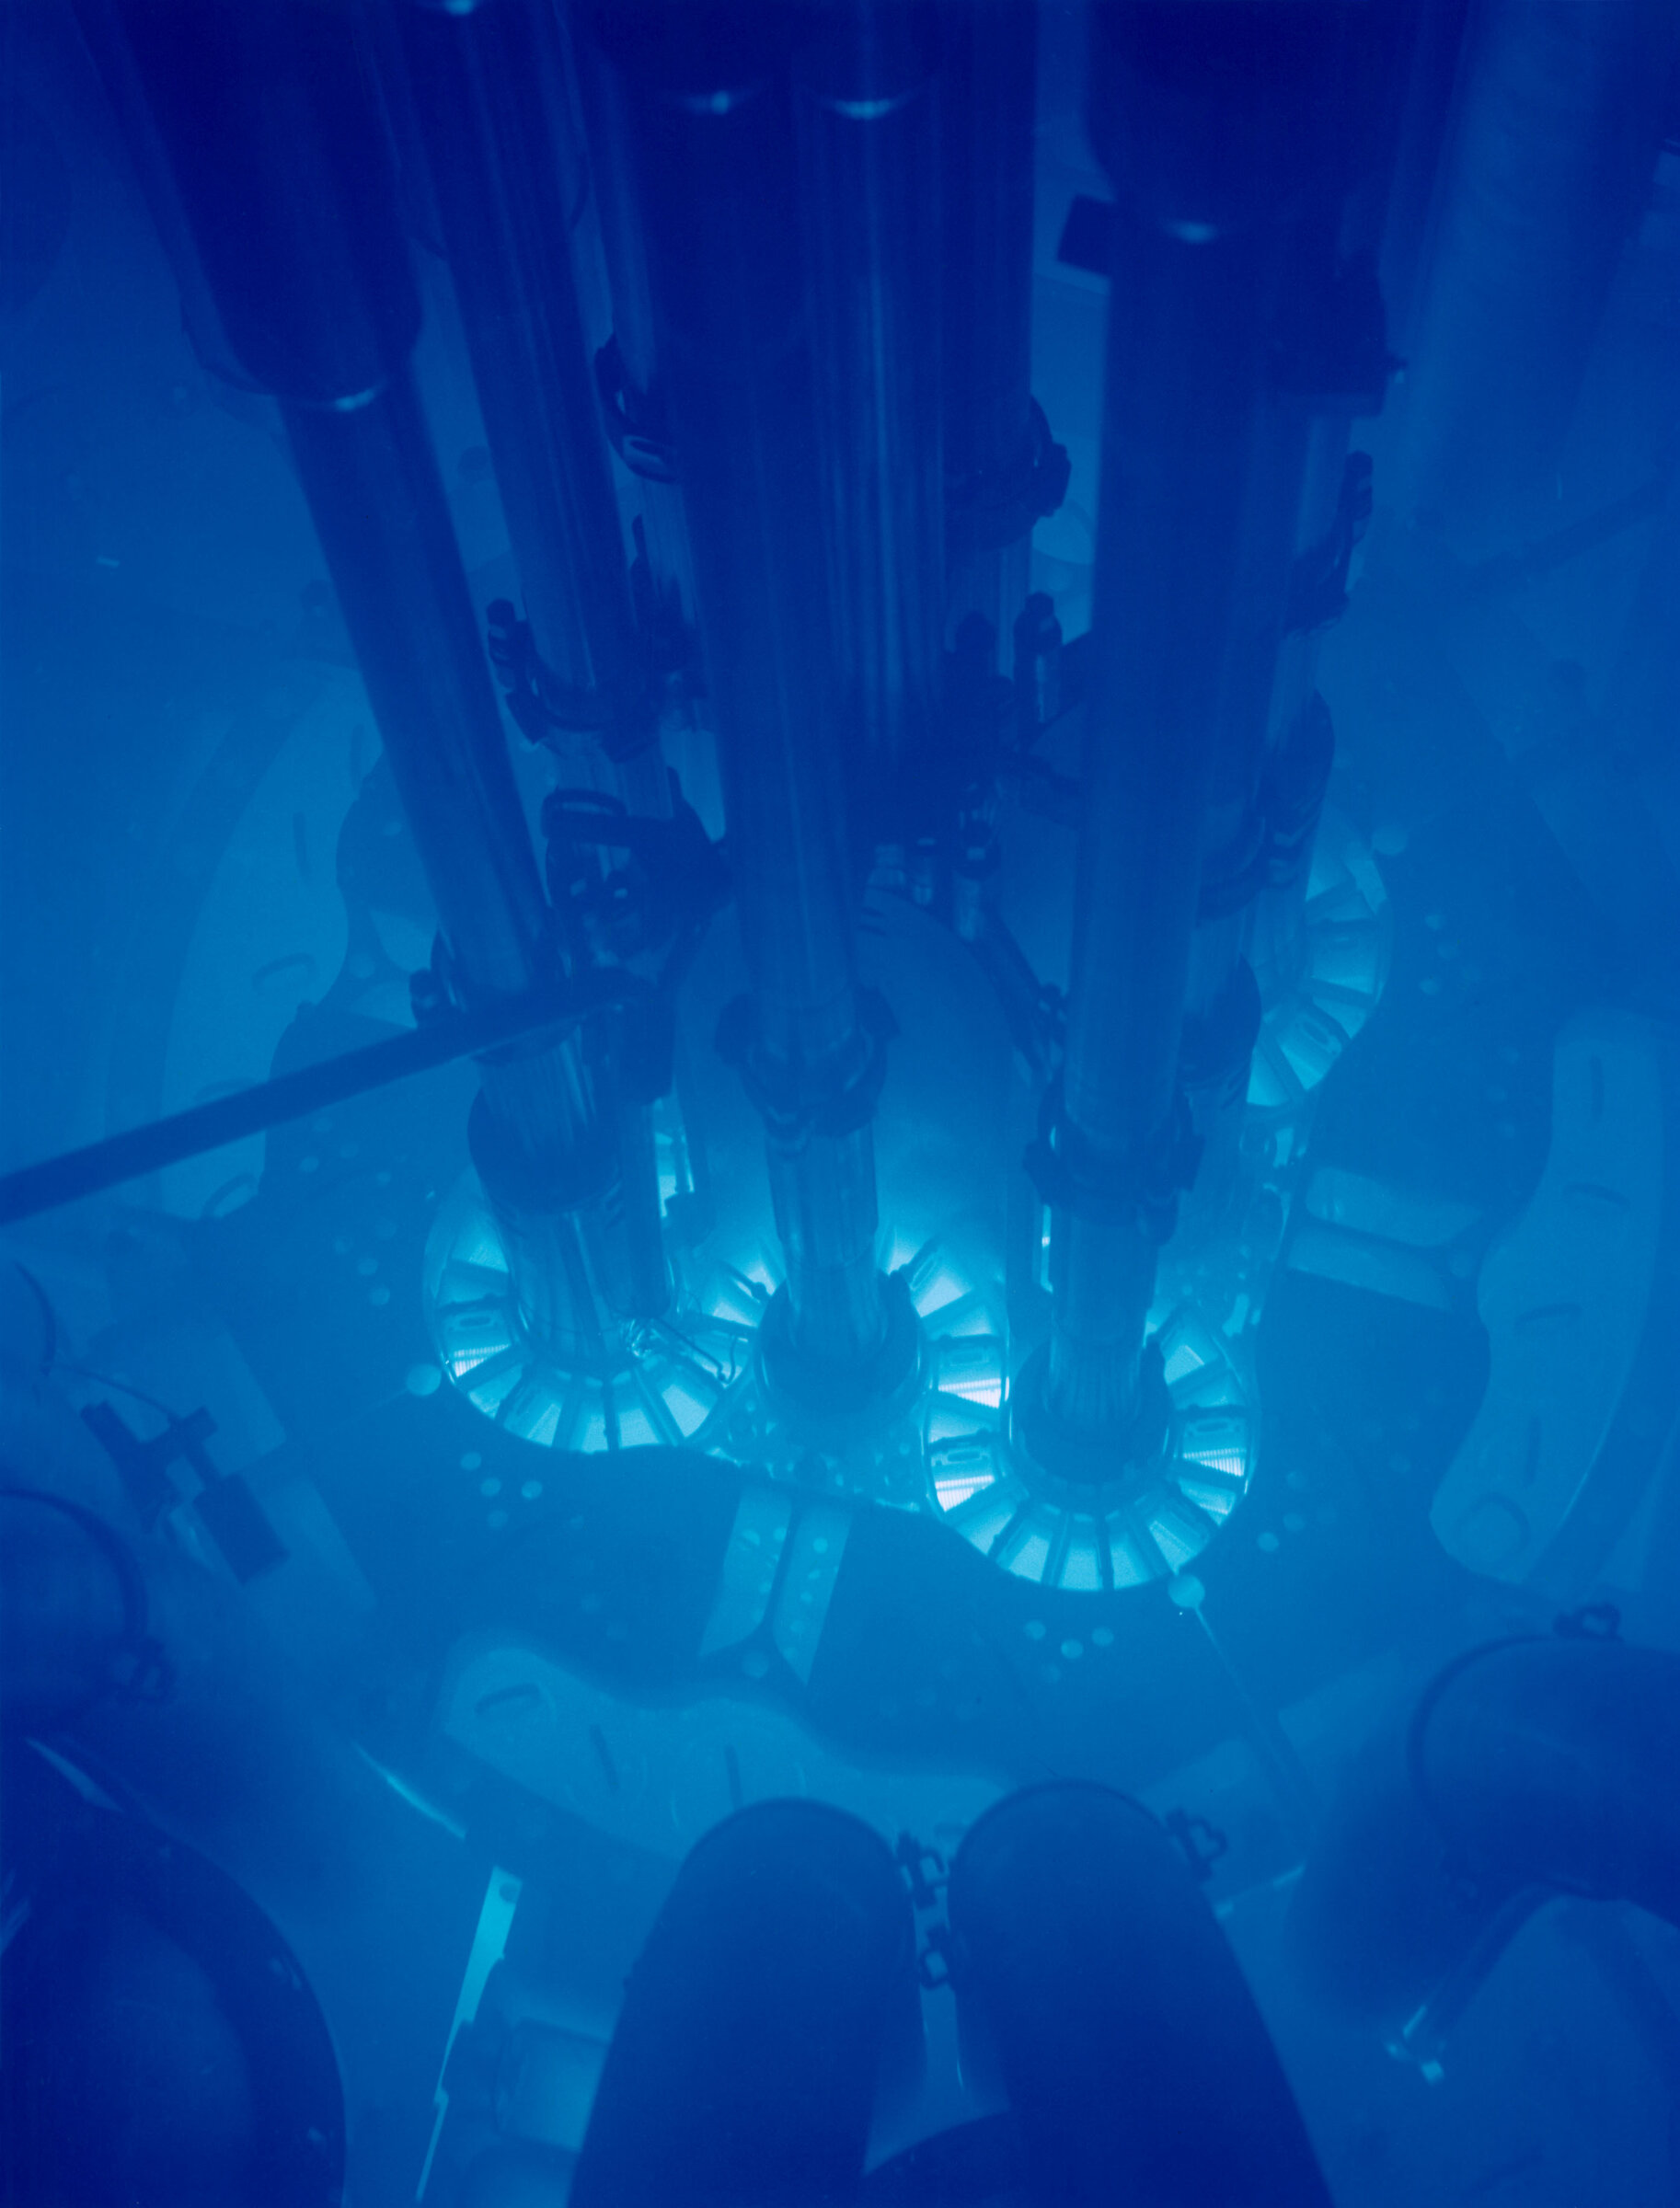
\includegraphics[height=2.1cm]{externas/cherenkov_reactor_ATR.jpg}\\[1pt]
      {\scriptsize Brillo Cherenkov en un reactor}\\[4pt]
      \begin{clave}
        Para emitir hay que ir más rápido que la luz en el agua
        ($\beta>0{,}75$): un electrón necesita \textbf{0,26\,MeV}, un muón
        \textbf{54\,MeV}. Luego emite $\sim$300 fotones/cm.
      \end{clave}
  \end{columns}
  \creditoizq{Fotos: US Navy (dom.\ público); Argonne Natl.\ Lab., CC BY-SA 2.0}
\end{frame}

% ---------------------------------------------------------------- 31
\begin{frame}{Qué medimos realmente: trazas, tiempos y una función lateral}
  \begin{columns}[c,onlytextwidth]
    \column{0.46\textwidth}
      \centering
      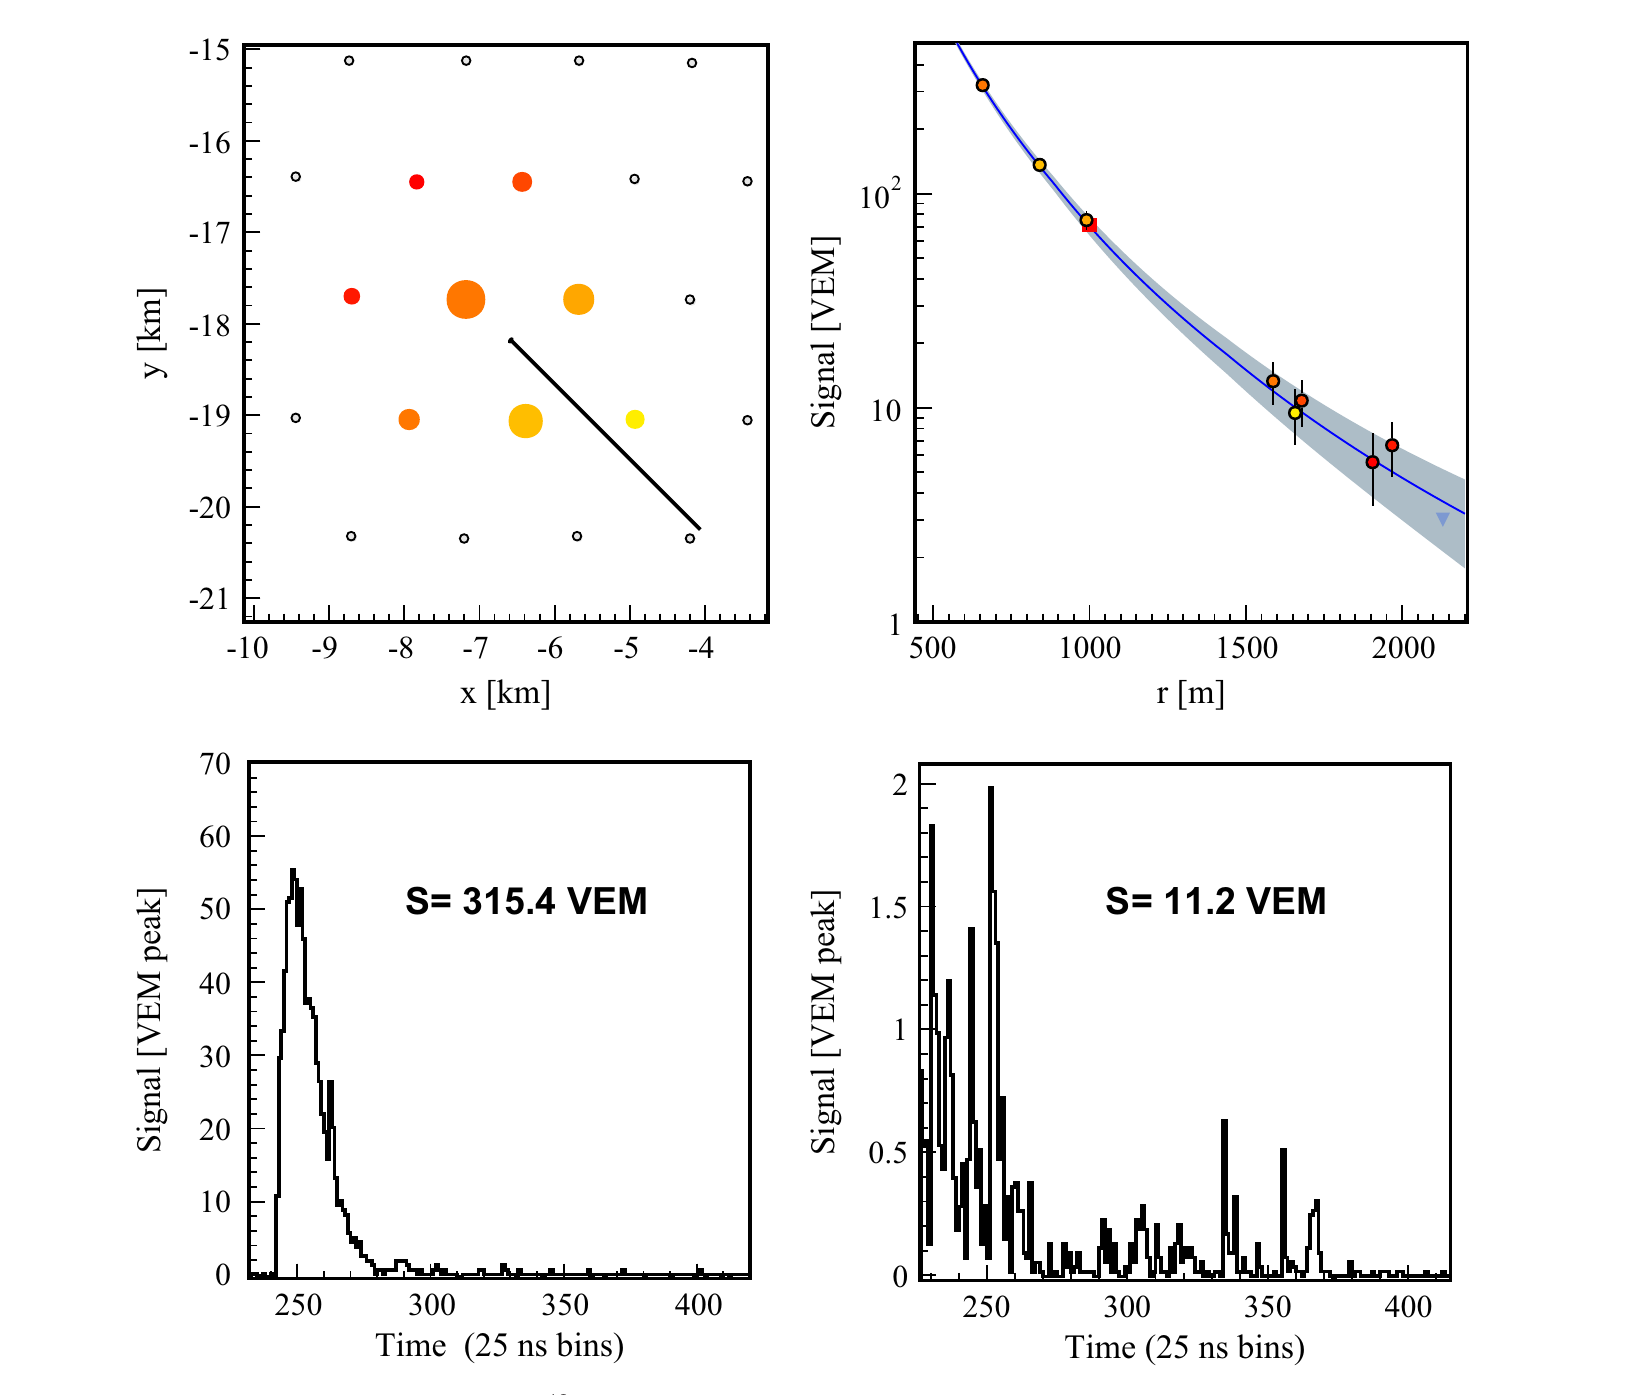
\includegraphics[width=\linewidth]{externas/auger_sd_evento_trazas.png}
    \column{0.51\textwidth}
      \small
      Evento de $\sim3\times10^{19}$\,eV, $\theta=28^\circ$, 8 estaciones.
      \begin{enumerate}\footnotesize
        \item \textbf{Trazas} cada 25\,ns, en \textbf{VEM}: cerca del núcleo un
          pulso grande; lejos, muones aislados.
        \item \textbf{Tiempos} de arribo $\to$ frente de la lluvia $\to$
          dirección ($\sim$1$^\circ$).
        \item \textbf{Señales} $\to$ función lateral $\to$ $S(1000)$ $\to$
          \textbf{energía} (calibrada con el FD).
      \end{enumerate}
      \begin{clave}
        Nunca vemos el primario: \textbf{inferimos} energía, dirección y masa
        desde sus secundarios, con incertezas estadísticas y sistemáticas.
      \end{clave}
  \end{columns}
  \credito{Figura: Colaboración Pierre Auger, NIM A 798 (2015) 172, Fig.~17}
\end{frame}

% ---------------------------------------------------------------- 32
\begin{frame}{Muones: mensajeros de la cascada hadrónica}
  \begin{columns}[c,onlytextwidth]
    \column{0.46\textwidth}
      \centering
      \begin{tikzpicture}[x=1cm,y=0.82cm]
        \draw[itedaGray!50, line width=6pt] (-0.2,-2.65) -- (5.2,-2.65);
        \node[font=\tiny, text=itedaGray, anchor=north west] at (-0.2,-2.75) {suelo};
        \node[font=\small] (h) at (0.4,1.8) {$\pi^\pm$};
        \draw[flecha, itedaTealDark] (0,2.6) -- (h);
        \node[font=\tiny, text=itedaGray, anchor=east] at (0,2.5) {cascada};
        \draw[flecha, itedaOrange, very thick] (h) -- (3.9,-2.55) node[pos=0.55, right, font=\small] {$\mu^\pm$};
        \draw[flecha, violetaNu, dashed] (h) -- (2.4,1.4) node[right, font=\small] {$\nu_\mu$};
        \node[font=\scriptsize, align=left, anchor=west] at (2.6,0.4)
          {$c\tau_\pi = 7{,}8$\,m:\\decae o interactúa};
        \node[font=\scriptsize, align=left, anchor=west] at (3.0,-1.2)
          {$\gamma c\tau_\mu\approx 6$\,km\\a 1\,GeV};
      \end{tikzpicture}\\[4pt]
      {\footnotesize La \textbf{dilatación temporal} los deja llegar
      ($c\tau_\mu=659$\,m); pierden $\sim$2\,GeV en el aire y casi no se desvían.}
    \column{0.51\textwidth}
      \small
      \textbf{Por qué importan}
      \begin{itemize}\footnotesize
        \item $N_\mu\propto A^{1-\beta}E^{\beta}$: sensibles a la \textbf{masa}.
        \item Guardan la memoria de la cascada \textbf{hadrónica}: física de
          partículas a $\sqrt{s}\sim100$\,TeV.
      \end{itemize}
      \begin{clave}
        \textbf{El enigma de los muones}: los datos tienen más señal hadrónica
        que las simulaciones, un factor $1{,}33\pm0{,}16$ (EPOS-LHC) a
        $1{,}61\pm0{,}21$ (QGSJet-II-04) a 6--16\,EeV.
      \end{clave}
  \end{columns}
  \credito{Auger, PRL 117 (2016) 192001}
\end{frame}

% ---------------------------------------------------------------- 33
\begin{frame}{El detector subterráneo de muones (UMD)}
  \begin{columns}[c,onlytextwidth]
    \column{0.43\textwidth}
      \centering
      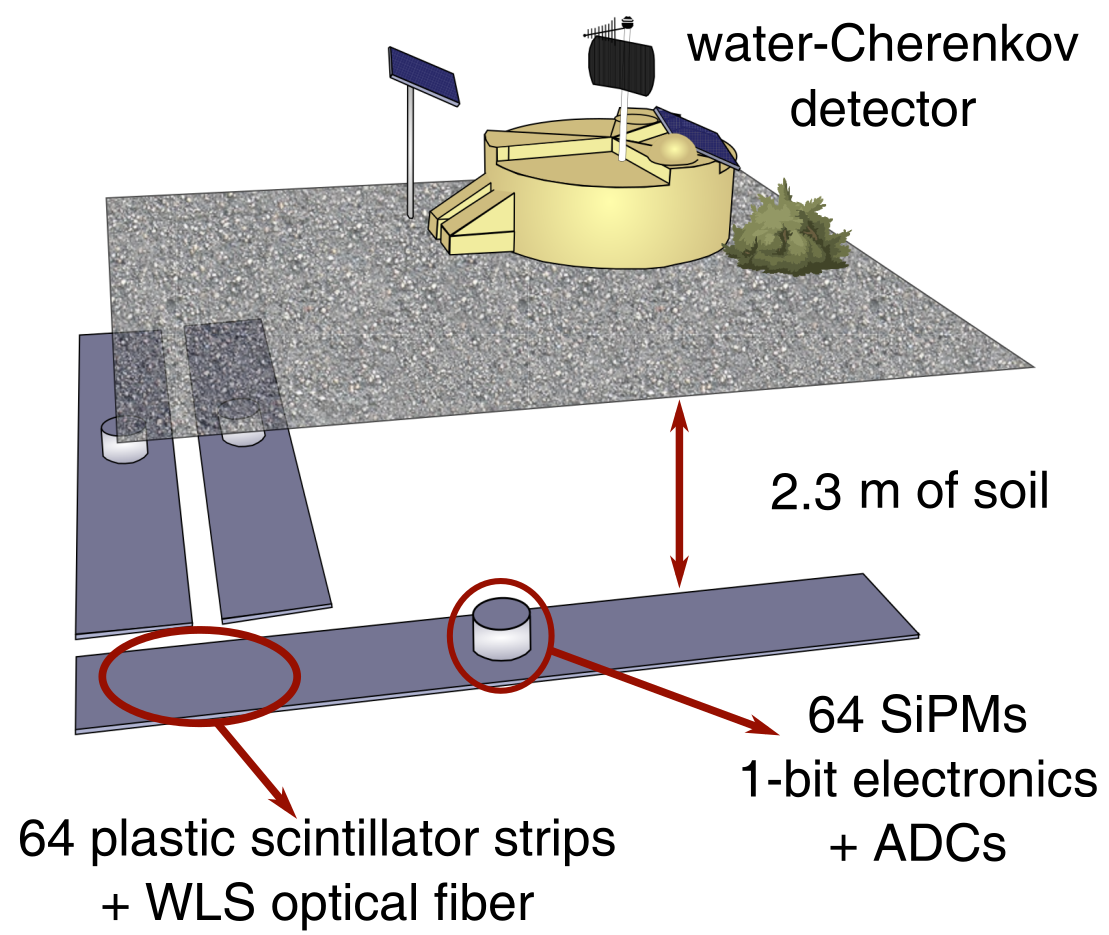
\includegraphics[width=0.82\linewidth]{tesis/umd.png}\\[2pt]
      \begin{itemize}\footnotesize
        \item 3 módulos de 10\,m$^2$ a \textbf{2,3\,m bajo tierra}
          ($\approx$540\,g/cm$^2$): umbral $\sim$1\,GeV$/\cos\theta$.
        \item 64 tiras de \textbf{centellador} por módulo, leídas con SiPMs.
      \end{itemize}
    \column{0.54\textwidth}
      \centering
      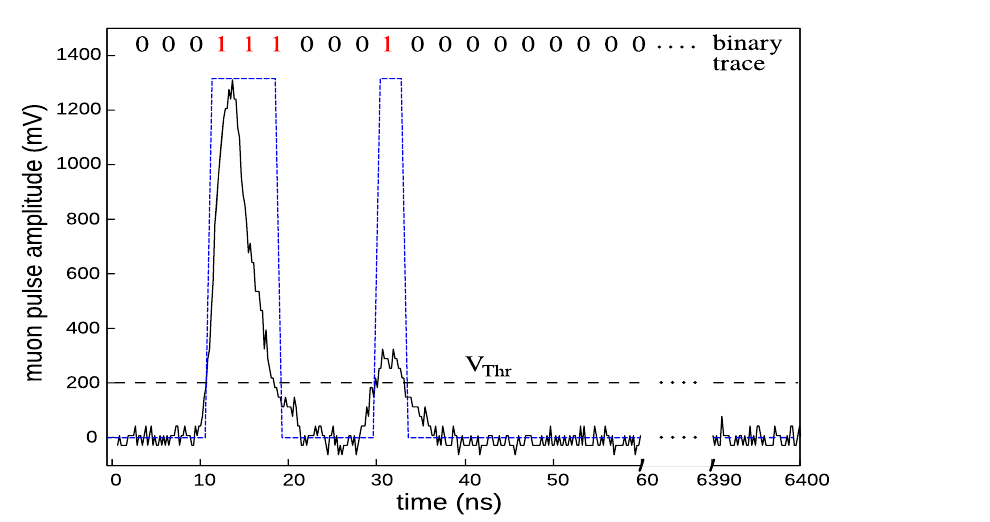
\includegraphics[width=0.85\linewidth]{externas/umd_traza_binaria.png}\\[1pt]
      {\scriptsize Pulso de un muón, discriminado y muestreado cada 3,125\,ns}\\[3pt]
      \begin{clave}
        \textbf{No es Cherenkov}: el muón ioniza y el plástico
        \textbf{centellea}. Cada tira es un contador: un patrón «1x1» es un
        muón y se \textbf{cuentan}. A alta densidad, se integra la carga.
      \end{clave}
  \end{columns}
  \credito{Esquema: Botti (2019). Traza: Colaboración Pierre Auger, EPJC 80 (2020) 751, Fig.~3}
\end{frame}

% ======================================================================
% BLOQUE 4 — Mi trabajo de licenciatura
% ======================================================================
\section{Mi tesis}
\bloque{MI TESIS · UMD}

% ---------------------------------------------------------------- 34
\begin{frame}{¿Se ve la asimetría con muones puros?}
  \begin{columns}[c,onlytextwidth]
    \column{0.46\textwidth}
      \centering
      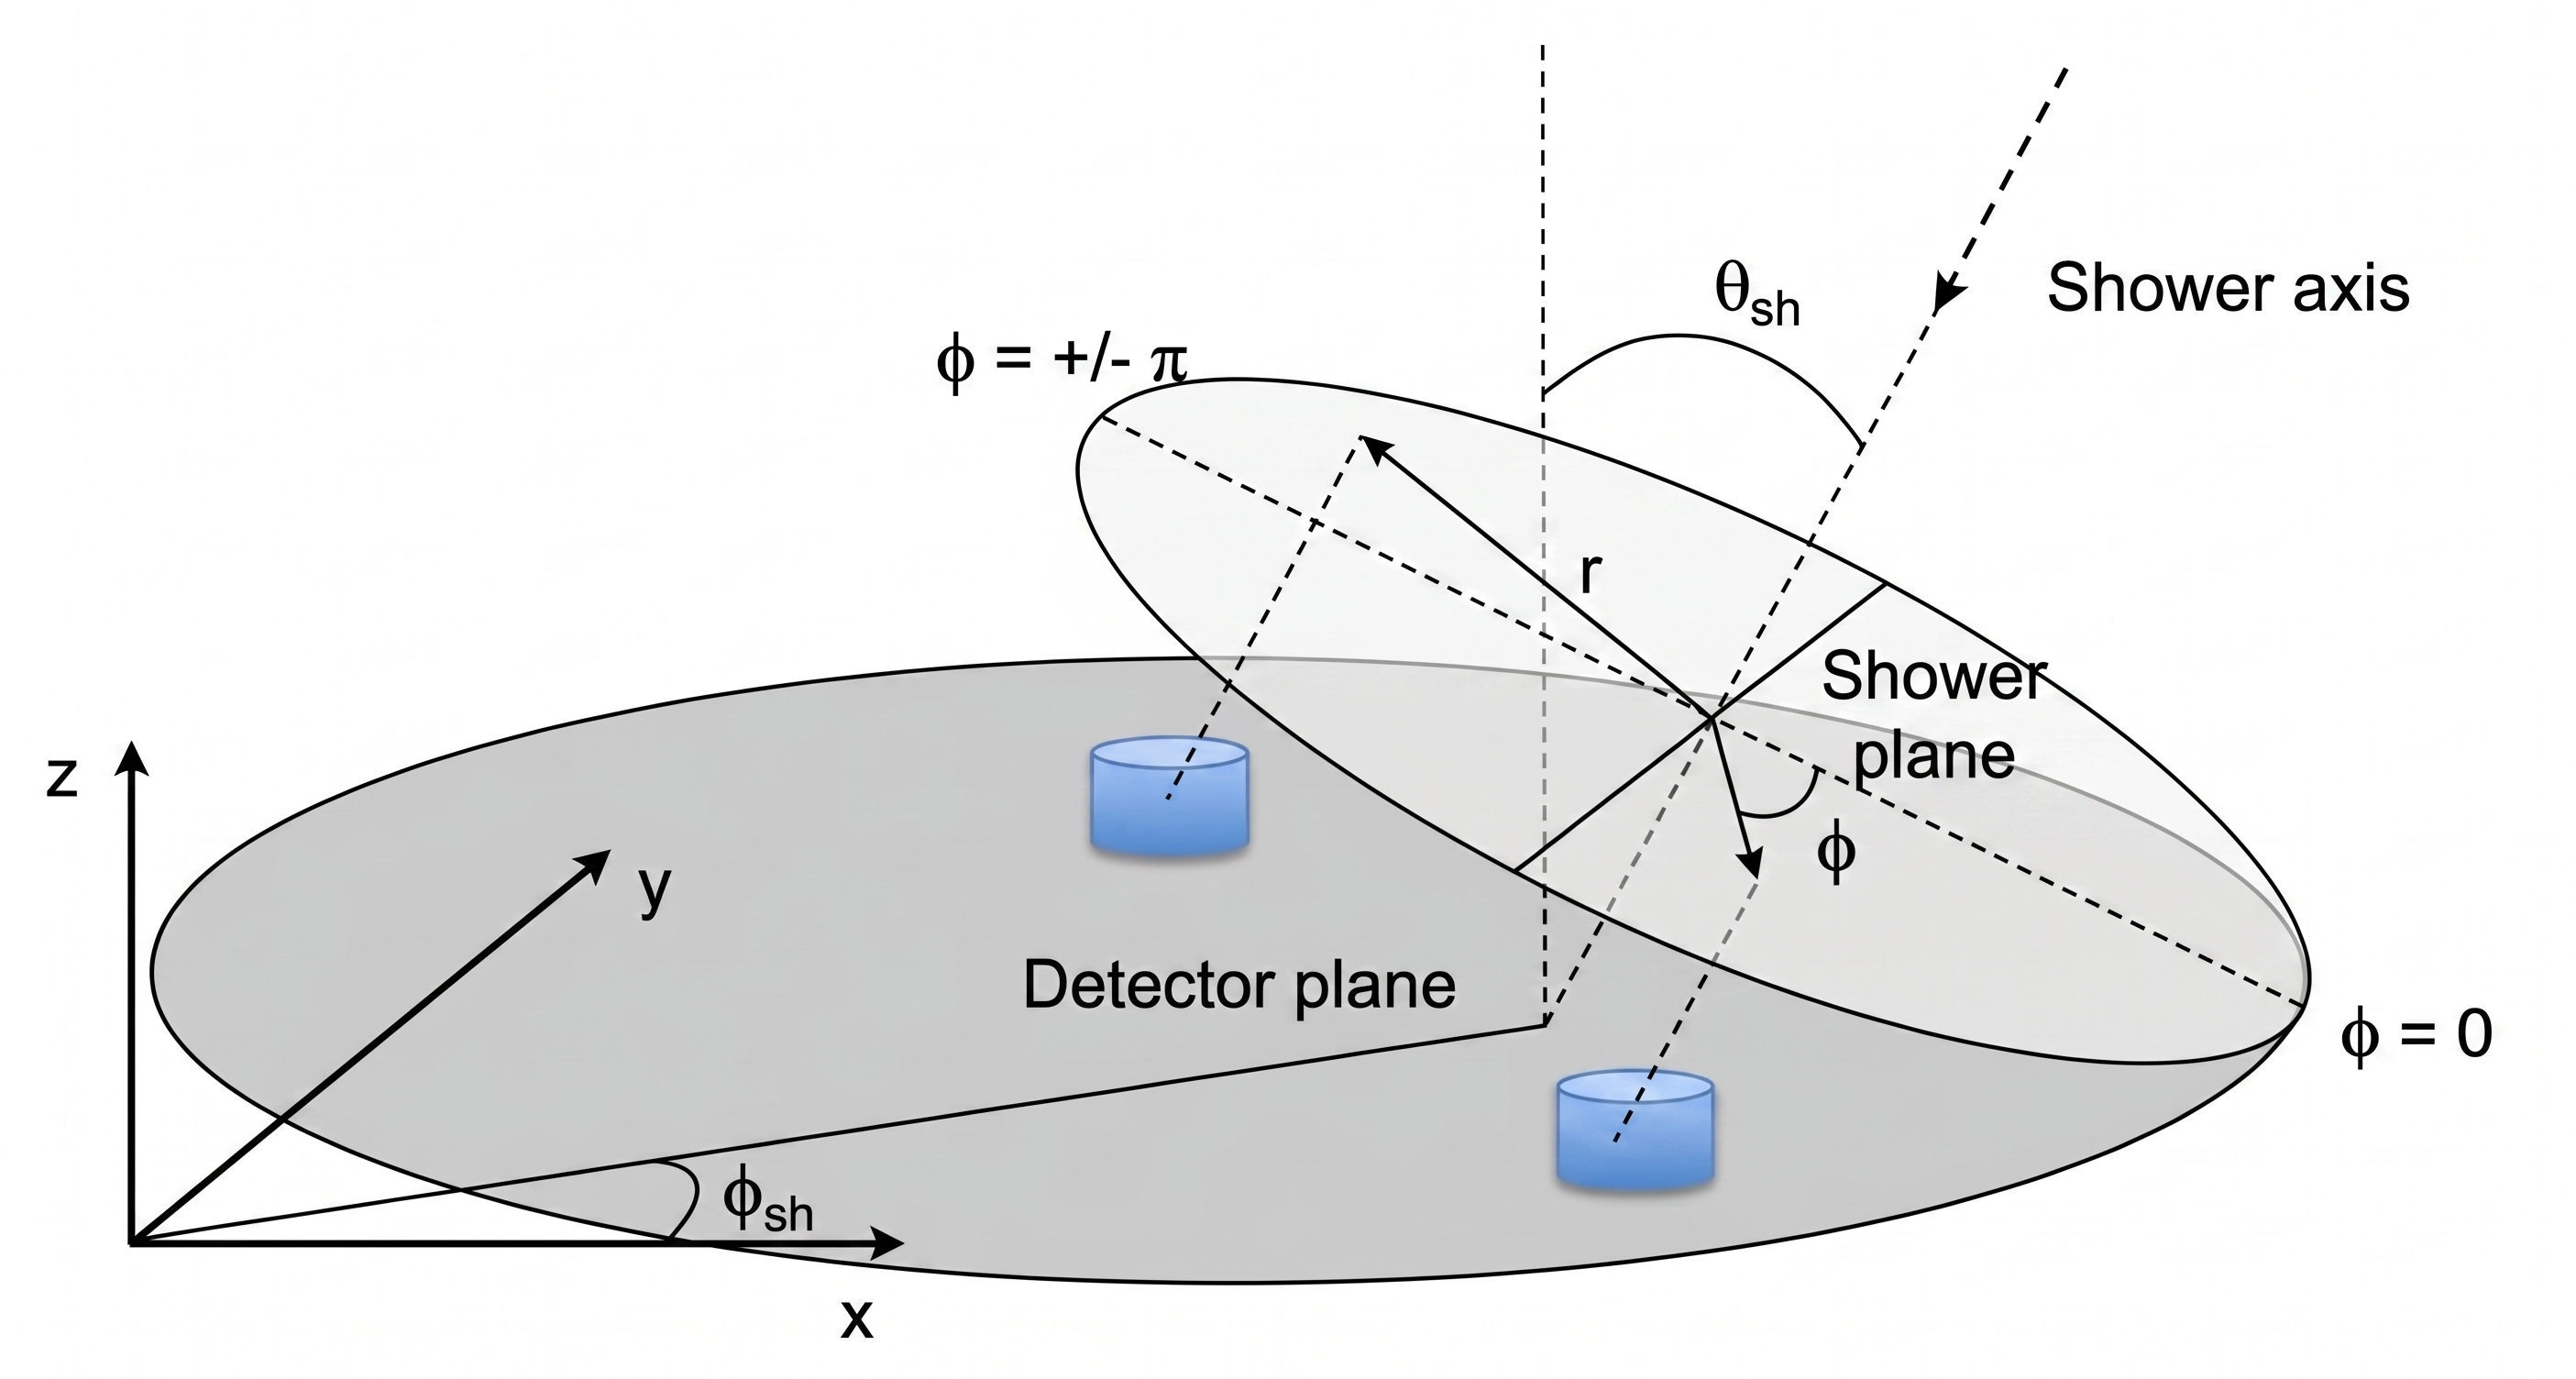
\includegraphics[width=0.92\linewidth]{tesis/esquema_lluvia.jpeg}\\[2pt]
      {\footnotesize Plano de la lluvia: $\phi=0$ es la región
      \textbf{temprana}, $\phi=\pm180^\circ$ la \textbf{tardía}.}
    \column{0.51\textwidth}
      \small
      En una lluvia inclinada la densidad en el suelo deja de ser circular:
      \[ \rho(\phi)=\rho_0\,\big(1+A_1\cos\phi\big) \]
      \begin{itemize}\footnotesize
        \item En el SD, $A_1$ de la señal \textbf{total} correlaciona con
          $X_\mathrm{max}$, pero mezcla electrones y muones.
        \item \textbf{Nunca se había estudiado con muones aislados}.
      \end{itemize}
      \vspace{-2pt}
      \begin{clave}
        \textbf{Objetivo}: caracterizar $A_1(r,\theta,E,A)$ en el UMD.
      \end{clave}
  \end{columns}
  \credito{Esquema: tesis de licenciatura (Silva Pizzi, FCEN-UBA, 2026), Cap.~3}
\end{frame}

% ---------------------------------------------------------------- 35
\begin{frame}{Cómo lo estudié}
  \begin{columns}[c,onlytextwidth]
    \column{0.50\textwidth}
      \begin{tikzpicture}[x=1cm,y=1cm,
        paso/.style={rounded corners=2pt, fill=itedaTeal, text=white,
          font=\scriptsize\bfseries, minimum height=0.62cm, inner sep=3pt, align=center},
        nota/.style={font=\tiny, text=itedaTealDark, align=left, anchor=west}]
        \node[paso] (a) at (0,3.0) {CORSIKA};
        \node[paso] (b) at (0,1.9) {Offline};
        \node[paso] (c) at (0,0.8) {Python};
        \node[paso, fill=itedaOrange] (d) at (0,-0.3) {ajuste de $A_1$};
        \draw[flecha, itedaGray] (a) -- (b); \draw[flecha, itedaGray] (b) -- (c);
        \draw[flecha, itedaGray] (c) -- (d);
        \node[nota] at (0.9,3.0) {lluvias de $p$, He, O, Fe; $10^{17{,}5}$--$10^{18}$\,eV;\\
          SIBYLL 2.3e, QGSJET-III.01, EPOS-LHC-R};
        \node[nota] at (0.9,1.9) {respuesta del SD y del UMD;\\reconstrucción como en los datos};
        \node[nota] at (0.9,0.8) {densidad de muones por módulo,\\en bines de $(r,\theta)$};
        \node[nota] at (1.25,-0.3) {primer armónico, errores \emph{bootstrap}};
      \end{tikzpicture}\\[6pt]
      \footnotesize
      \textbf{Dos geometrías de detector}: el \textbf{Anillo Denso} (12
      estaciones virtuales a 450\,m, cada 30$^\circ$) y el arreglo real de
      750\,m.\\[2pt]
      \textbf{Dos geometrías de lluvia}: la \textbf{verdadera} (MC) y la
      \textbf{reconstruida} (REC).
    \column{0.47\textwidth}
      \centering
      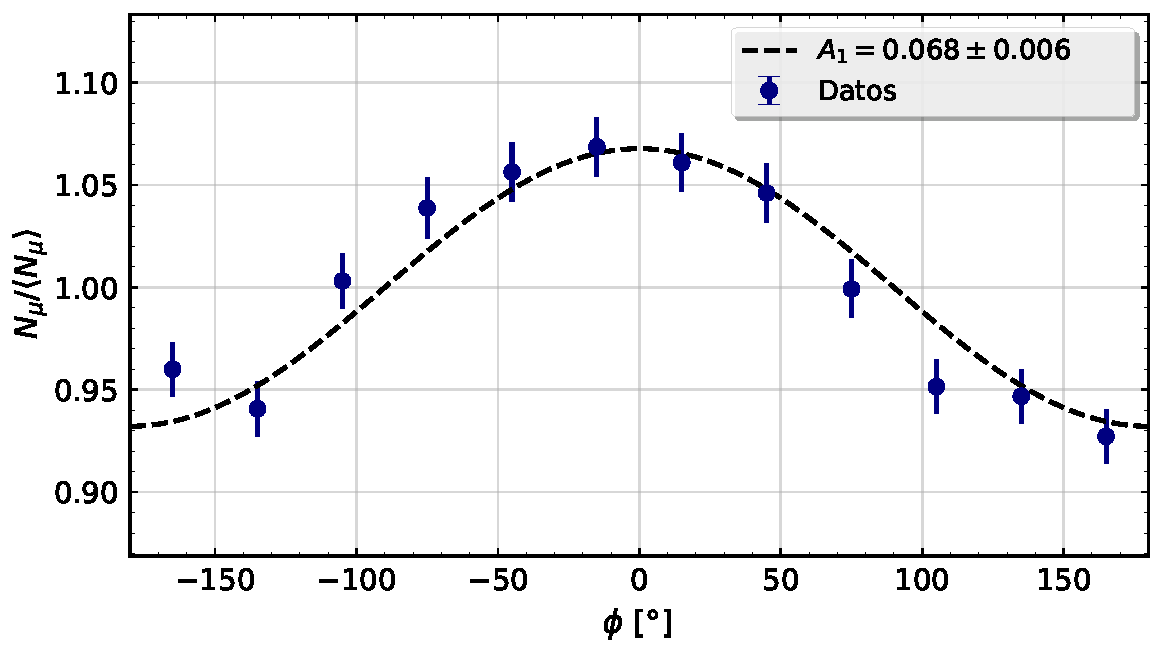
\includegraphics[width=\linewidth]{tesis/Ajuste_UMD_REC_Bin9.pdf}\\[1pt]
      {\footnotesize Anillo Denso, protones, $59^\circ$--$65^\circ$: la
      densidad de muones \textbf{reconstruida} sigue un coseno, con
      $\pm7\%$ entre regiones.}
  \end{columns}
  \credito{Figura: tesis, Cap.~5}
\end{frame}

% ---------------------------------------------------------------- 36
\begin{frame}{La asimetría sobrevive en los muones}
  \begin{columns}[T,onlytextwidth]
    \column{0.49\textwidth}
      \centering
      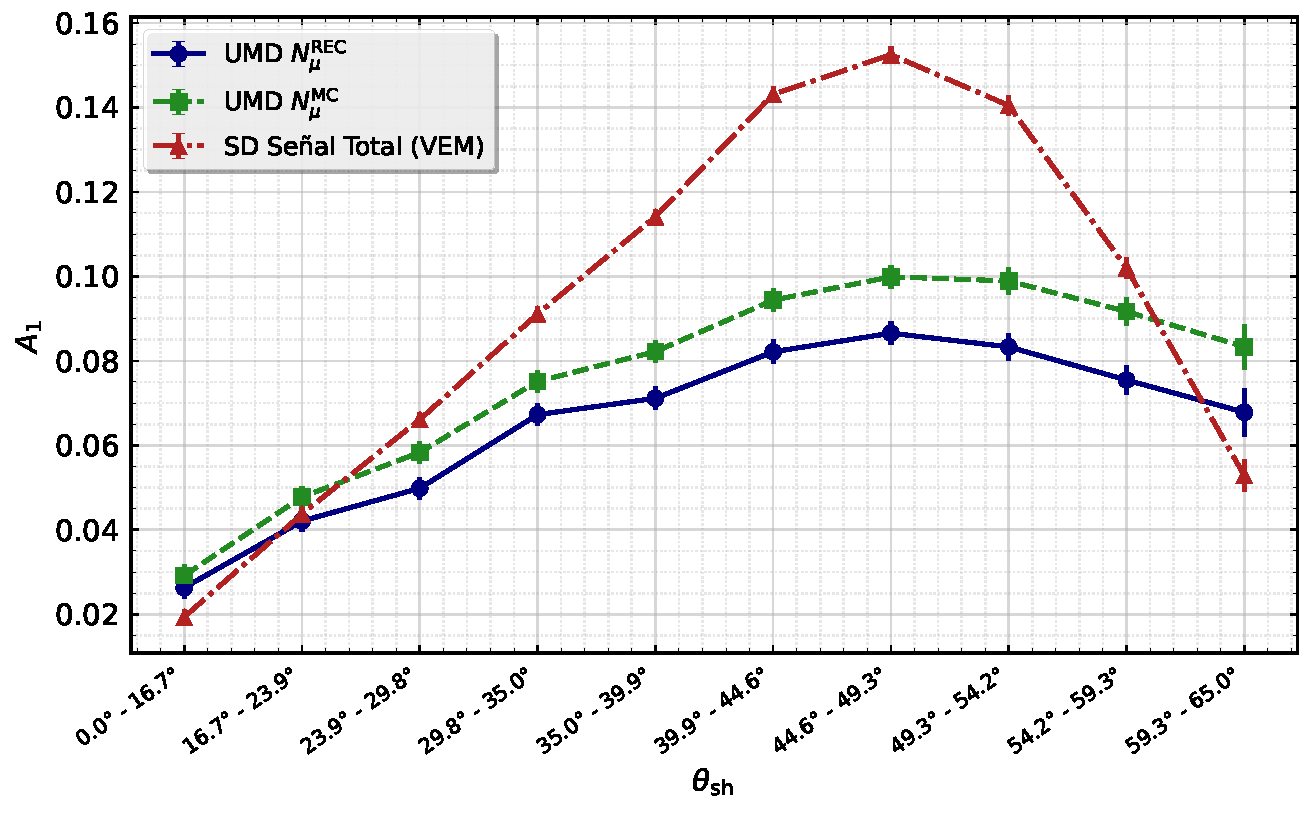
\includegraphics[width=0.88\linewidth]{tesis/Evolucion_Asimetria_vs_Theta.pdf}\\[1pt]
      {\footnotesize Crece con $\theta$: $A_1\approx0{,}09$ a 45--50$^\circ$,
      sin componente electromagnética.}
    \column{0.49\textwidth}
      \centering
      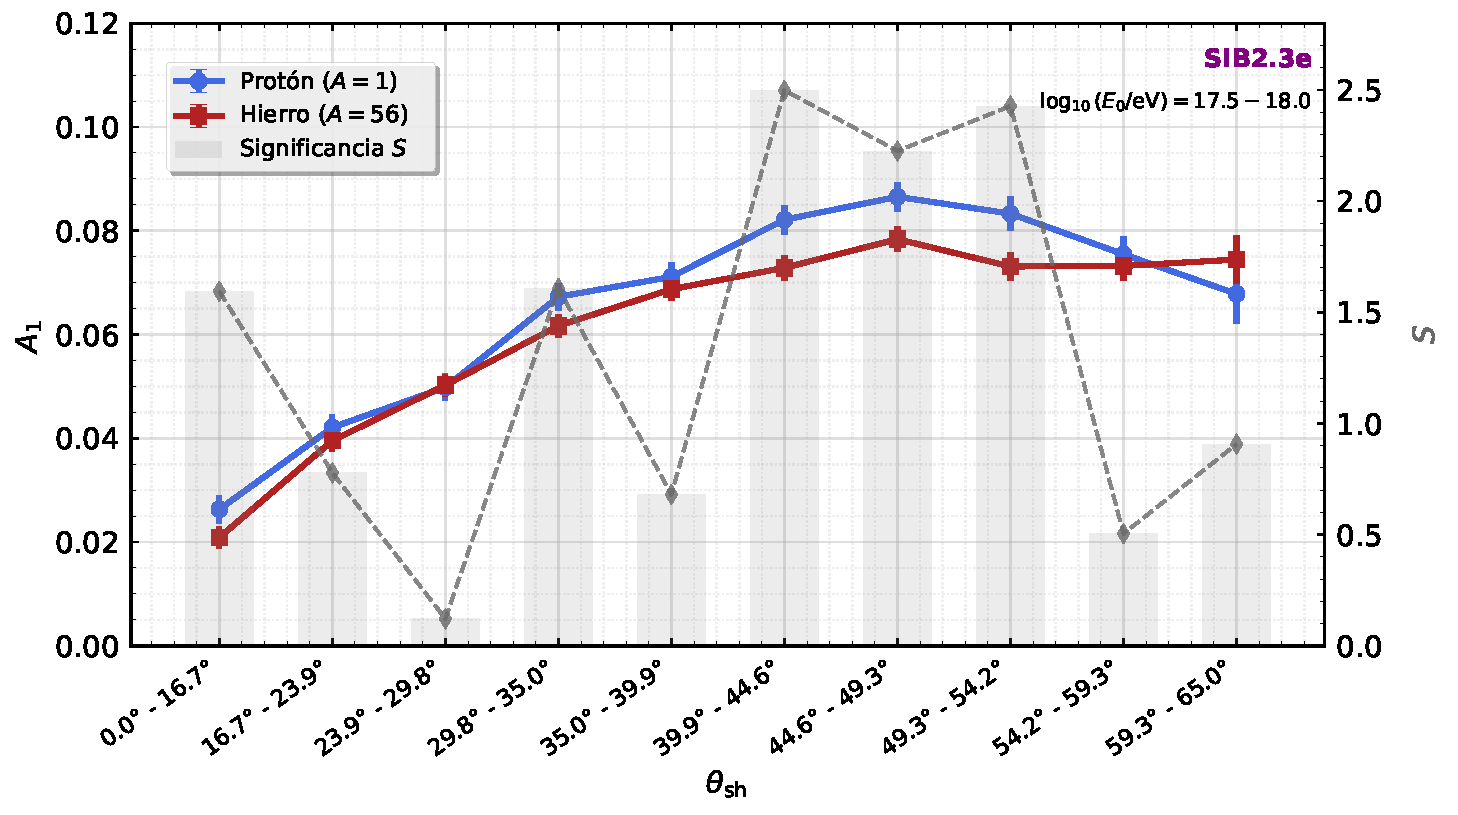
\includegraphics[width=0.88\linewidth]{tesis/Mass_Discrimination_MF.pdf}\\[1pt]
      {\footnotesize Protón por encima de hierro: diferencia de medias
      $\sim$2,5 veces su incerteza a 40--55$^\circ$.}
  \end{columns}
  \vspace{2pt}
  \begin{clave}
    $A_1\propto (r/D)\tan\theta$: un primario liviano acerca la producción
    de muones al suelo (menor $D$) y \textbf{aumenta} la modulación.
  \end{clave}
  \creditoizq{Figuras: tesis, Cap.~5 (Anillo Denso, SIBYLL 2.3e, $10^{17{,}5}$--$10^{18}$\,eV)}
\end{frame}

% ---------------------------------------------------------------- 37
\begin{frame}{Hallazgo 1: un sesgo de selección en el SD}
  \begin{columns}[c,onlytextwidth]
    \column{0.48\textwidth}
      \centering
      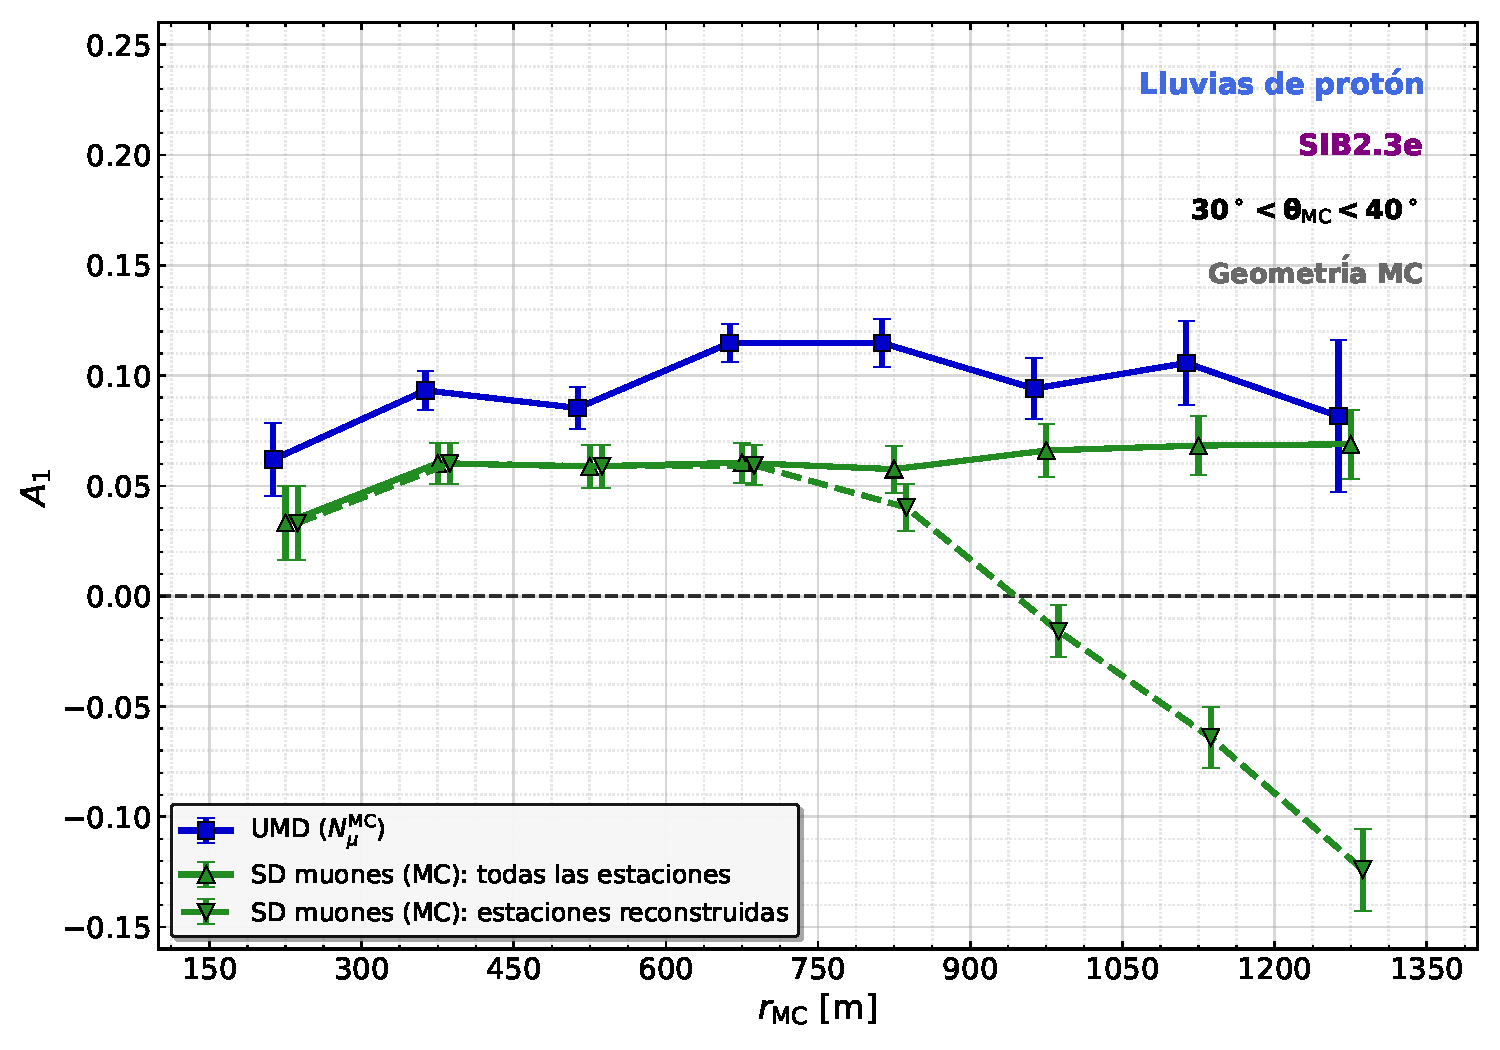
\includegraphics[width=\linewidth]{tesis/SD_Seleccion_Estaciones_vs_UMD.pdf}\\[1pt]
      {\footnotesize Mismos conteos de muones, mismo ajuste: sólo cambia
      \textbf{sobre qué estaciones se promedia}.}
    \column{0.49\textwidth}
      \centering
      \begin{tikzpicture}[x=1cm,y=1cm]
        \tikzset{
          tanque/.style={thick, fill=itedaLight, draw=itedaTeal},
          fuera/.style={thick, dashed, fill=white, draw=itedaGray!60},
          em/.style={fill=itedaOrange}, mu/.style={fill=itedaTealDark}}
        \node[font=\scriptsize\bfseries, text=cmbAzul] at (1.25,2.4) {región temprana};
        \node[font=\scriptsize\bfseries, text=cmbRojo] at (4.05,2.4) {región tardía};
        % temprana: las tres disparan (mucha señal EM); 0, 1 y 2 muones
        \foreach \x in {0,0.9,1.8}{
          \draw[tanque] (\x,0.9) rectangle ++(0.7,1.1);
          \foreach \k in {0.17,0.29,0.41,0.53}{\fill[em] (\x+\k,1.78) circle (1.2pt);}
          \node[font=\scriptsize, text=verdeRadio] at (\x+0.35,0.65) {\faCheck};}
        \fill[mu] (0.9+0.35,1.2) circle (2pt);
        \fill[mu] (1.8+0.22,1.2) circle (2pt); \fill[mu] (1.8+0.48,1.2) circle (2pt);
        % tardía: poca señal EM; sólo dispara la que tiene muones
        \draw[fuera] (2.8,0.9) rectangle ++(0.7,1.1);
        \draw[tanque] (3.7,0.9) rectangle ++(0.7,1.1);
        \draw[fuera] (4.6,0.9) rectangle ++(0.7,1.1);
        \foreach \x in {2.8,3.7,4.6}{\fill[em] (\x+0.35,1.78) circle (1.2pt);}
        \fill[mu] (3.7+0.22,1.2) circle (2pt); \fill[mu] (3.7+0.48,1.2) circle (2pt);
        \node[font=\scriptsize, text=cmbRojo] at (2.8+0.35,0.65) {\faTimes};
        \node[font=\scriptsize, text=verdeRadio] at (3.7+0.35,0.65) {\faCheck};
        \node[font=\scriptsize, text=cmbRojo] at (4.6+0.35,0.65) {\faTimes};
        \node[font=\tiny, anchor=west] at (0,0.2) {\textcolor{itedaOrange}{$\bullet$} $e^\pm,\gamma$
          \quad \textcolor{itedaTealDark}{$\bullet$} $\mu$ \quad
          \textcolor{verdeRadio}{\faCheck}\ forma parte del evento};
        \node[font=\scriptsize] at (1.25,-0.3) {$\langle N_\mu\rangle_\mathrm{sel}=1$};
        \node[font=\scriptsize] at (4.05,-0.3) {$\langle N_\mu\rangle_\mathrm{sel}=2$};
      \end{tikzpicture}\\[2pt]
      {\footnotesize La señal EM hace entrar estaciones tempranas con pocos
      muones; del lado tardío sólo entran las ricas en muones.}
  \end{columns}
  \creditoizq{Protones, SIBYLL 2.3e, $30^\circ$--$40^\circ$, geometría MC. Figura: tesis, Cap.~6}
\end{frame}

% ---------------------------------------------------------------- 38
\begin{frame}{Hallazgo 2: el núcleo reconstruido se corre}
  \centering
  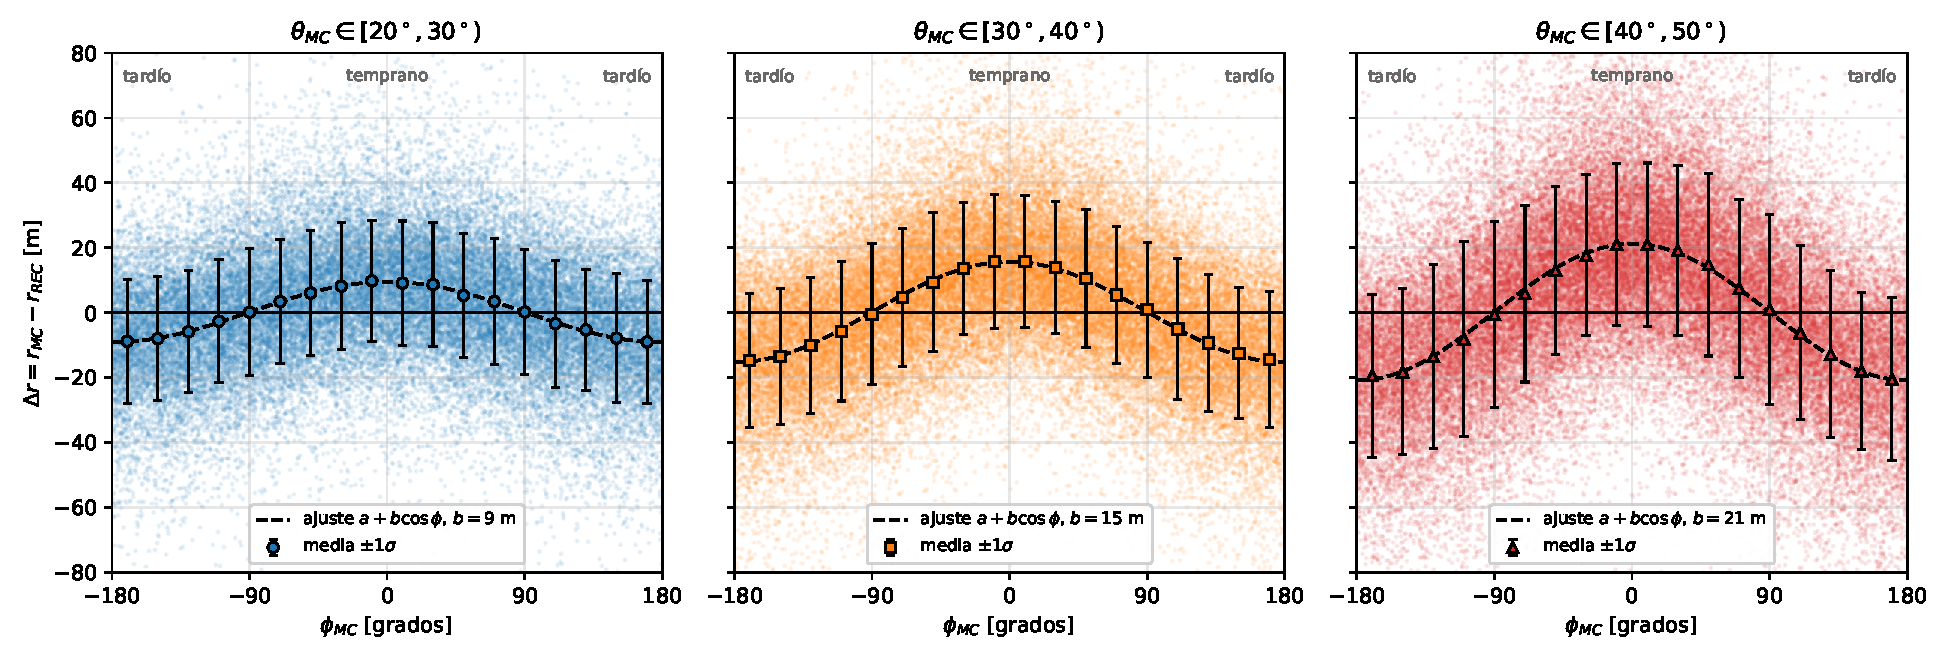
\includegraphics[width=0.7\linewidth]{tesis/corrimiento_nucleo_azimut.pdf}\\[0pt]
  \begin{columns}[T,onlytextwidth]
    \column{0.42\textwidth}
      \small
      Una función lateral \textbf{simétrica} ajustada a una señal
      \textbf{asimétrica} acerca el núcleo al exceso temprano ($b\simeq9$, 15,
      21\,m). Con $\rho\propto r^{-\beta}$: \;$\Delta A_1\simeq-\beta\,b/r$.
    \column{0.55\textwidth}
      {\scriptsize
      \begin{tabular}{@{}lcccc@{}}
        \toprule
        $\theta$ & $A_1$ (MC) & $A_1$ (REC) & $\Delta A_1$ obs. & $-\beta b/r$ \\
        \midrule
        20--30$^\circ$ & 0,062 & 0,011 & $-0{,}051$ & $-0{,}051$ \\
        30--40$^\circ$ & 0,086 & 0,002 & $-0{,}084$ & $-0{,}081$ \\
        40--50$^\circ$ & 0,108 & $-0{,}002$ & $-0{,}110$ & $-0{,}102$ \\
        \bottomrule
      \end{tabular}}\\[3pt]
      {\footnotesize 450--600\,m. La \textbf{distancia} explica casi toda la
      pérdida: un sesgo \textbf{estimable}, no ruido.}
  \end{columns}
  \creditoizq{Figura y tabla: tesis, Cap.~5 y 6. Núcleo verdadero menos reconstruido, en función del azimut}
\end{frame}

% ---------------------------------------------------------------- 39
\begin{frame}{Primera mirada a los datos de campo}
  \begin{columns}[c,onlytextwidth]
    \column{0.56\textwidth}
      \centering
      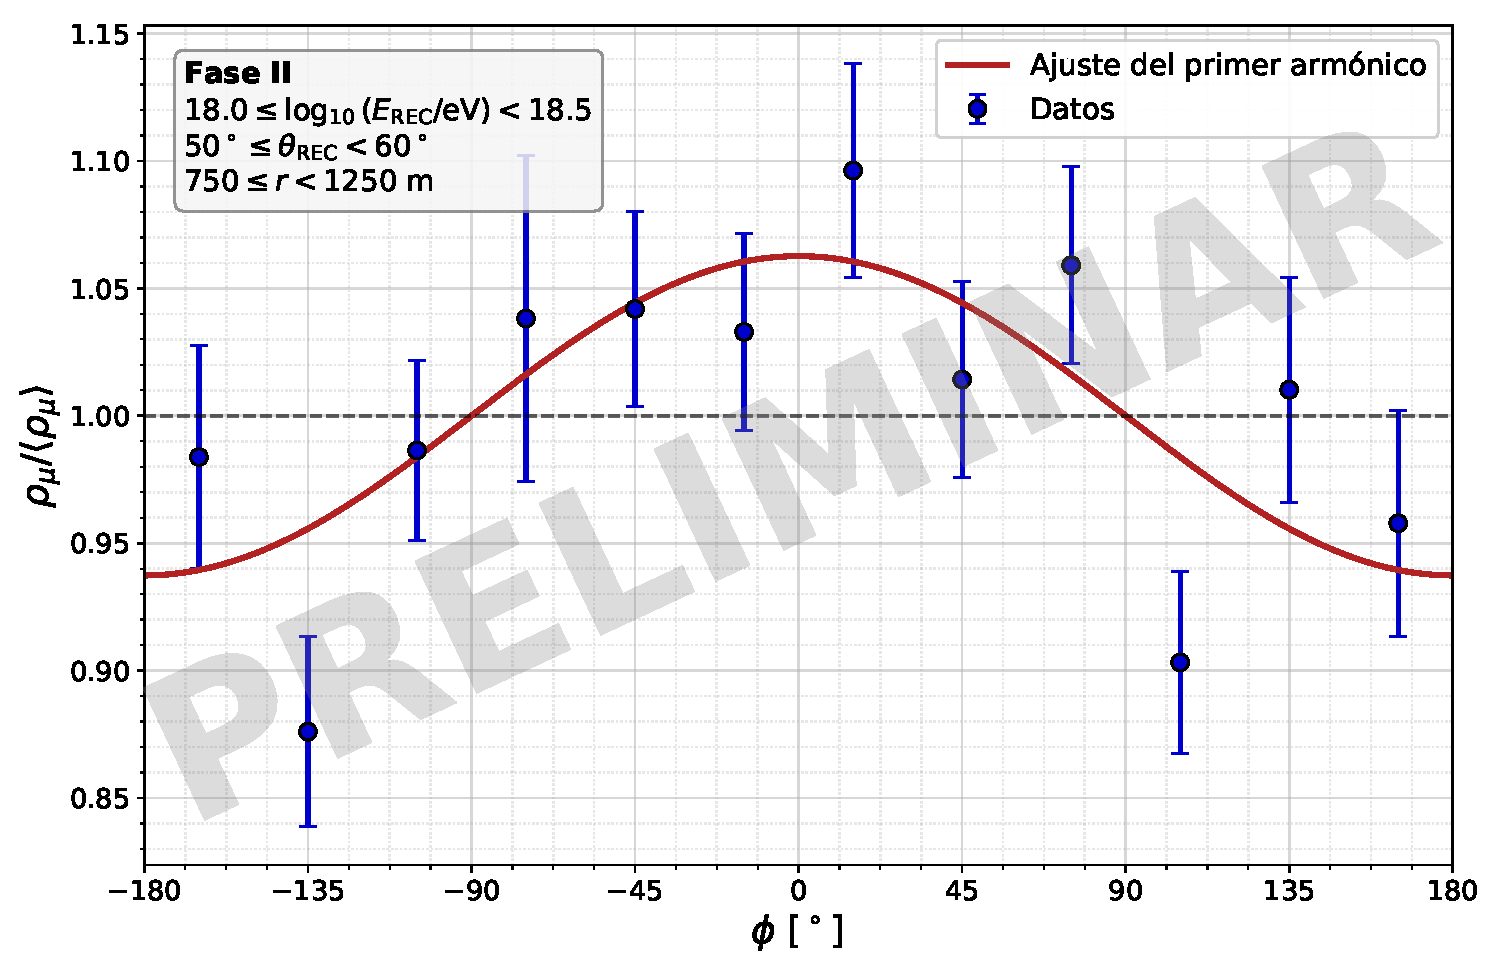
\includegraphics[width=\linewidth]{tesis/datos_campo_preliminar.pdf}
    \column{0.41\textwidth}
      \small
      UMD, arreglo de 750\,m, Fase II.\\
      {\footnotesize $18{,}0\le\lg(E/\mathrm{eV})<18{,}5$, \;$50^\circ\le\theta<60^\circ$,
      \;$750\le r<1250$\,m}
      \[ A_1 = 0{,}063\pm0{,}017 \]
      {\footnotesize Máximo en la región temprana, como predicen las
      simulaciones. Faltan los sistemáticos.}\\[4pt]
      \begin{clave}
        Hasta donde sabemos, la primera observación de esta asimetría con
        \textbf{muones aislados} de la componente electromagnética.
      \end{clave}

  \end{columns}
  \begin{tikzpicture}[remember picture, overlay]
    \node[anchor=north east] at ([xshift=-0.3cm, yshift=-1.1cm]current page.north east) {\preliminar};
  \end{tikzpicture}
  \credito{Datos de la Colaboración Pierre Auger; análisis propio (tesis, Cap.~6). Resultado preliminar, no oficial.}
\end{frame}

% ---------------------------------------------------------------- 40
\begin{frame}{Desde Argentina, a la región y al mundo}
  \begin{columns}[c,onlytextwidth]
    \column{0.36\textwidth}
      \centering
      \begin{tikzpicture}
        \mapaSA{6.4cm}
        \tikzset{lugar/.style={fill=itedaOrange, draw=white, line width=0.9pt},
          rot/.style={font=\scriptsize\bfseries, text=white, fill=noche,
            fill opacity=0.7, text opacity=1, inner sep=1.2pt, rounded corners=1pt}}
        \filldraw[lugar] \geoSA{-58.4}{-34.6} circle (2.6pt);
        \node[rot, anchor=west] at \geoSA{-57.5}{-35.3} {Buenos Aires};
        \filldraw[lugar] \geoSA{-69.6}{-35.5} circle (2.6pt);
        \node[rot, anchor=east] at \geoSA{-70.6}{-36.0} {Malargüe};
        \filldraw[lugar] \geoSA{-65.8}{-28.5} circle (2.6pt);
        \node[rot, anchor=east] at \geoSA{-67.0}{-28.2} {Catamarca};
        \filldraw[lugar] \geoSA{-46.6}{-23.5} circle (2.6pt);
        \node[rot, anchor=west] at \geoSA{-45.5}{-24.2} {São Paulo};
        \filldraw[lugar] \geoSA{-35.2}{-5.8} circle (2.6pt);
        \node[rot, anchor=north] at \geoSA{-37.5}{-7.0} {Natal};
      \end{tikzpicture}
    \column{0.61\textwidth}
      \begin{tikzpicture}[x=1cm,y=0.82cm]
        \draw[itedaGray, thick] (0,0.3) -- (0,-5.4);
        \foreach \y/\f/\t in {
            0/{mar.\ 2026}/{\textbf{Reunión de la Colaboración Pierre Auger}: el encuentro de toda la colaboración, dos veces por año},
            -1.05/{jun.\ 2026}/{\textbf{SAMMA}: School on Astroparticle and Multi-messenger Astrophysics, ICTP-SAIFR, São Paulo},
            -2.1/{jul.\ 2026}/{\textbf{IDPASC School 2026}, Instituto Internacional de Física (UFRN), Natal},
            -3.15/{sep.\ 2026}/{\textbf{RAFA 2026}, Catamarca},
            -4.2/{nov.\ 2026}/{\textbf{Reunión de la Colaboración Pierre Auger}, presentando los resultados de la tesis}}{
          \fill[itedaOrange] (0,\y) circle (2.4pt);
          \node[font=\scriptsize\bfseries, anchor=east, text=itedaOrange] at (-0.15,\y) {\f};
          \node[font=\scriptsize, anchor=west, text width=7.6cm, align=left] at (0.15,\y) {\t};}
      \end{tikzpicture}\\[6pt]
      \begin{clave}
        Hacer física desde Argentina te conecta con la comunidad
        \textbf{latinoamericana} y con colaboraciones \textbf{internacionales}
        de cientos de investigadores.
      \end{clave}
      {\scriptsize\color{itedaGray} Tesis en ITeDA (2025--26), dirigida por
      J.\,M.~Figueira y F.~Sánchez; defensa en FCEN-UBA, octubre de 2026.}
  \end{columns}
  \creditoizq{Mapa: Natural Earth (dominio público)}
\end{frame}

% ======================================================================
% BLOQUE 5 — Neutrinos, IceCube y astronomía multimensajero
% ======================================================================
\section{Neutrinos e IceCube}
\bloque{NEUTRINOS}

% ---------------------------------------------------------------- 41
\begin{frame}[plain]
  \fondo[0.0]{halzen/halzen_p005_sintexto.jpg}
  \velo[0.9]{b}
  \begin{tikzpicture}[remember picture, overlay]
    \node[anchor=north west, text=white, font=\Large\bfseries]
      at ([xshift=0.6cm, yshift=-0.35cm]current page.north west)
      {¿Por qué neutrinos? La portada, explicada};
    \tikzset{rot/.style={font=\small\bfseries, align=left, text=white}}
    \node[rot, anchor=south] at ([xshift=8.7cm, yshift=7.2cm]current page.south west)
      {$p$: desviado por campos magnéticos};
    \node[rot, anchor=south west] at ([xshift=9.2cm, yshift=4.7cm]current page.south west)
      {$\gamma$: absorbido\\{\footnotesize $\gamma\gamma_\mathrm{fondo}\to e^+e^-$}};
    \node[rot, anchor=north, text=hielo] at ([xshift=9.0cm, yshift=3.6cm]current page.south west)
      {$\nu$: en línea recta y sin absorberse};
    \node[anchor=south west, text width=14.6cm, align=left, text=white, font=\small]
      at ([xshift=0.6cm, yshift=0.35cm]current page.south west) {%
      \textbf{Neutros}: no se desvían. \textbf{Interacción débil}: escapan de
      ambientes opacos a la luz. Se producen en \textbf{interacciones hadrónicas}:
      señalan dónde se aceleran protones y núcleos.\\[2pt]
      El precio: $\sigma_{\nu N}(1\,\mathrm{PeV})\sim10^{-33}\,\mathrm{cm^2}$,
      \;$\lambda$ en hielo $\sim2\times10^{4}$\,km: \textbf{en un km de hielo
      interactúa uno de cada $\sim$20.000.}};
  \end{tikzpicture}
  \creditoblanco{Composición: F.~Halzen, Erice 2024}
\end{frame}

% ---------------------------------------------------------------- 42
\begin{frame}{De dónde salen los neutrinos astrofísicos}
  \begin{columns}[c,onlytextwidth]
    \column{0.55\textwidth}
      \centering
      \begin{tikzpicture}[x=1cm,y=1cm]
        \node[font=\small\bfseries, text=itedaOrange] (p) at (0,1.5) {$p$};
        \node[font=\small, align=center] (t) at (0,0) {$p$ (gas)\\o $\gamma$ (luz)};
        \node[circle, fill=itedaLight, draw=itedaTeal, inner sep=2pt, font=\scriptsize] (v) at (1.6,0.75) {choque};
        \draw[flecha] (p) -- (v); \draw[flecha] (t) -- (v);
        \node[font=\small] (pi0) at (3.3,1.7) {$\pi^0$};
        \node[font=\small] (pic) at (3.3,-0.2) {$\pi^\pm$};
        \draw[flecha] (v) -- (pi0); \draw[flecha] (v) -- (pic);
        \node[font=\small, text=cmbAzul, anchor=west] (gg) at (4.4,1.7) {$\gamma\,\gamma$};
        \draw[flecha, cmbAzul] (pi0) -- (gg);
        \node[font=\small, anchor=west] (mu) at (4.4,0.4) {$\mu^\pm$};
        \node[font=\small, text=violetaNu, anchor=west] (n1) at (4.4,-0.8) {$\nu_\mu$};
        \draw[flecha] (pic) -- (mu.west); \draw[flecha, violetaNu] (pic) -- (n1.west);
        \node[font=\small, text=violetaNu, anchor=west] at (5.4,0.4) {$\to e^\pm\,\nu_e\,\nu_\mu$};
      \end{tikzpicture}\\[6pt]
      \small
      \[ E_\nu\approx\tfrac{1}{20}E_p, \qquad E_\gamma\approx\tfrac{1}{10}E_p \]
      {\footnotesize Sabores en la fuente $\nu_e:\nu_\mu:\nu_\tau\approx1:2:0$;
      tras oscilar en el viaje, $\approx1:1:1$ en la Tierra.}
    \column{0.42\textwidth}
      \begin{clave}
        \textbf{Por cada neutrino, un fotón gamma}: los mismos piones producen
        ambos. Si una fuente emite neutrinos sin los gammas esperados, la
        fuente es \textbf{opaca} a la luz.
      \end{clave}
      \vspace{4pt}
      {\footnotesize Un neutrino es la firma de \textbf{hadrones} acelerados;
      un gamma puede venir también de electrones (Compton inverso).}
  \end{columns}
\end{frame}

% ---------------------------------------------------------------- 43
\begin{frame}{Auger también busca neutrinos}
  \begin{columns}[c,onlytextwidth]
    \column{0.56\textwidth}
      \centering
      \begin{tikzpicture}[x=1cm,y=1cm]
        \fill[itedaGray!25] (-0.5,-1.2) -- (7,-1.2) -- (7,-0.2) -- (5.6,-0.2) --
          (4.6,0.9) -- (3.8,0.4) -- (3.0,-0.2) -- (-0.5,-0.2) -- cycle;
        \node[font=\tiny, text=itedaGray] at (4.4,0.2) {Andes};
        \draw[itedaTeal, thick] (-0.5,-0.2) -- (7,-0.2);
        \foreach \x in {0,0.6,...,2.4}{\fill[itedaTeal] (\x,-0.2) rectangle ++(0.18,0.12);}
        \draw[violetaNu, thick, dashed] (7.0,-0.75) -- (4.0,-0.55);
        \node[font=\scriptsize, text=violetaNu, anchor=south east] at (7.0,-0.75) {$\nu_\tau$};
        \draw[cmbRojo, thick, -{Stealth}] (4.0,-0.55) -- (3.2,-0.25)
          node[pos=0.3, below, font=\scriptsize] {$\tau$};
        \fill[itedaOrange] (3.1,-0.18) circle (1.5pt);
        \fill[itedaOrange!30] (3.1,-0.18) -- (0.2,0.35) -- (0.2,-0.18) -- cycle;
        \node[font=\scriptsize, align=center] at (2.1,0.75) {lluvia que «sube»\\casi horizontal};
        \draw[itedaTealDark, thick, -{Stealth}] (-0.4,2.5) -- (0.5,-0.1);
        \node[font=\scriptsize, align=left, anchor=west] at (-0.1,2.4)
          {$\nu$ descendente muy inclinado:\\lluvia \textbf{joven}, rica en $e^\pm$};
      \end{tikzpicture}\\[4pt]
      {\footnotesize Rozando la Tierra (y los Andes), un $\nu_\tau$ produce un
      $\tau$ que decae en el aire.}
    \column{0.41\textwidth}
      \small
      Las lluvias de rayos cósmicos muy inclinados llegan \textbf{viejas}:
      sólo muones. Una lluvia inclinada \textbf{joven} delata a un neutrino.
      \vspace{4pt}
      \begin{clave}
        Sin candidatos hasta hoy: límites entre los más restrictivos a EeV, y
        búsquedas en coincidencia con ondas gravitacionales (GW170817).
      \end{clave}
      {\footnotesize\color{itedaGray} Auger es un observatorio de
      lluvias, no un telescopio de neutrinos: su sensibilidad empieza en
      $\sim10^{17}$\,eV.}
  \end{columns}
  \creditoizq{Esquema ilustrativo, sin escala}
\end{frame}

% ---------------------------------------------------------------- 43b
\begin{frame}[plain]
  \fondo[0.0]{halzen/polo_sur_avion.jpg}
  \velo[0.7]{t}
  \begin{tikzpicture}[remember picture, overlay]
    \node[anchor=north west, text=white, align=left, text width=13cm]
      at ([xshift=0.6cm, yshift=-0.45cm]current page.north west) {%
      {\Large\bfseries El Polo Sur, desde un avión}\\[4pt]
      {\small Ese puntito es la base Amundsen--Scott, con el laboratorio de
      IceCube. Abajo hay casi \textbf{3\,km de hielo}, ultratransparente por
      debajo de 1,35\,km de profundidad.}};
    \draw[itedaOrange, very thick, -{Stealth[length=3mm]}]
      ([xshift=-4.2cm, yshift=-1.6cm]current page.center) -- ([xshift=-2.3cm, yshift=-0.35cm]current page.center);
    \node[text=white, font=\small\bfseries, anchor=north east, fill=black, fill opacity=0.45,
      text opacity=1, inner sep=2pt]
      at ([xshift=-4.1cm, yshift=-1.6cm]current page.center) {IceCube};
  \end{tikzpicture}
  \creditoblanco{Foto: vía F.~Halzen, Erice 2024}
\end{frame}

% ---------------------------------------------------------------- 44
\bloque{NEUTRINOS · ICECUBE}
\begin{frame}[plain]
  \fondo[0.1]{halzen/icecube_lab_aurora.jpg}
  \velo[0.85]{l}
  \begin{tikzpicture}[remember picture, overlay]
    \node[anchor=north west, text=white, align=left, text width=6.6cm]
      at ([xshift=0.6cm, yshift=-0.6cm]current page.north west) {%
      {\Large\bfseries IceCube: un kilómetro cúbico de hielo antártico}\\[10pt]
      \small\color{white}
      \begin{itemize}\small\color{white}
        \item 86 cuerdas, \textbf{5160 módulos ópticos} entre 1450 y 2450\,m de
          profundidad.
        \item Hielo ultratransparente: longitud de absorción de 100 a 250\,m.
        \item Completado en 2010; en el techo, IceTop mide lluvias.
      \end{itemize}};
    \node[anchor=east, fill=white, rounded corners=3pt, inner sep=3pt]
      at ([xshift=-0.5cm, yshift=-0.2cm]current page.east)
      {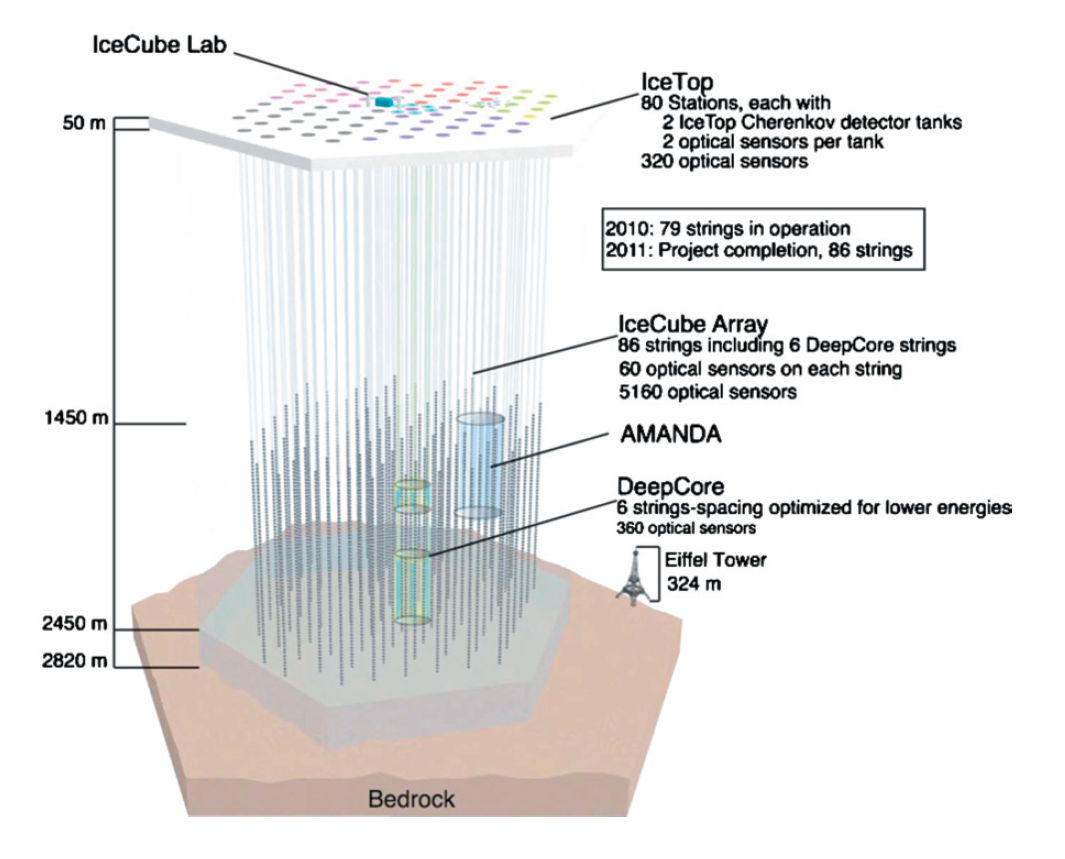
\includegraphics[height=6.1cm]{externas/icecube_arquitectura.png}};
  \end{tikzpicture}
  \creditoblanco{Foto: IceCube/NSF, vía F.~Halzen (2024). Diagrama: IceCube, CC BY 3.0 (Wikimedia Commons)}
\end{frame}

% ---------------------------------------------------------------- 45
\begin{frame}{Premio Nobel de Física 2026: Francis Halzen}
  \begin{columns}[c,onlytextwidth]
    \column{0.55\textwidth}
      \centering
      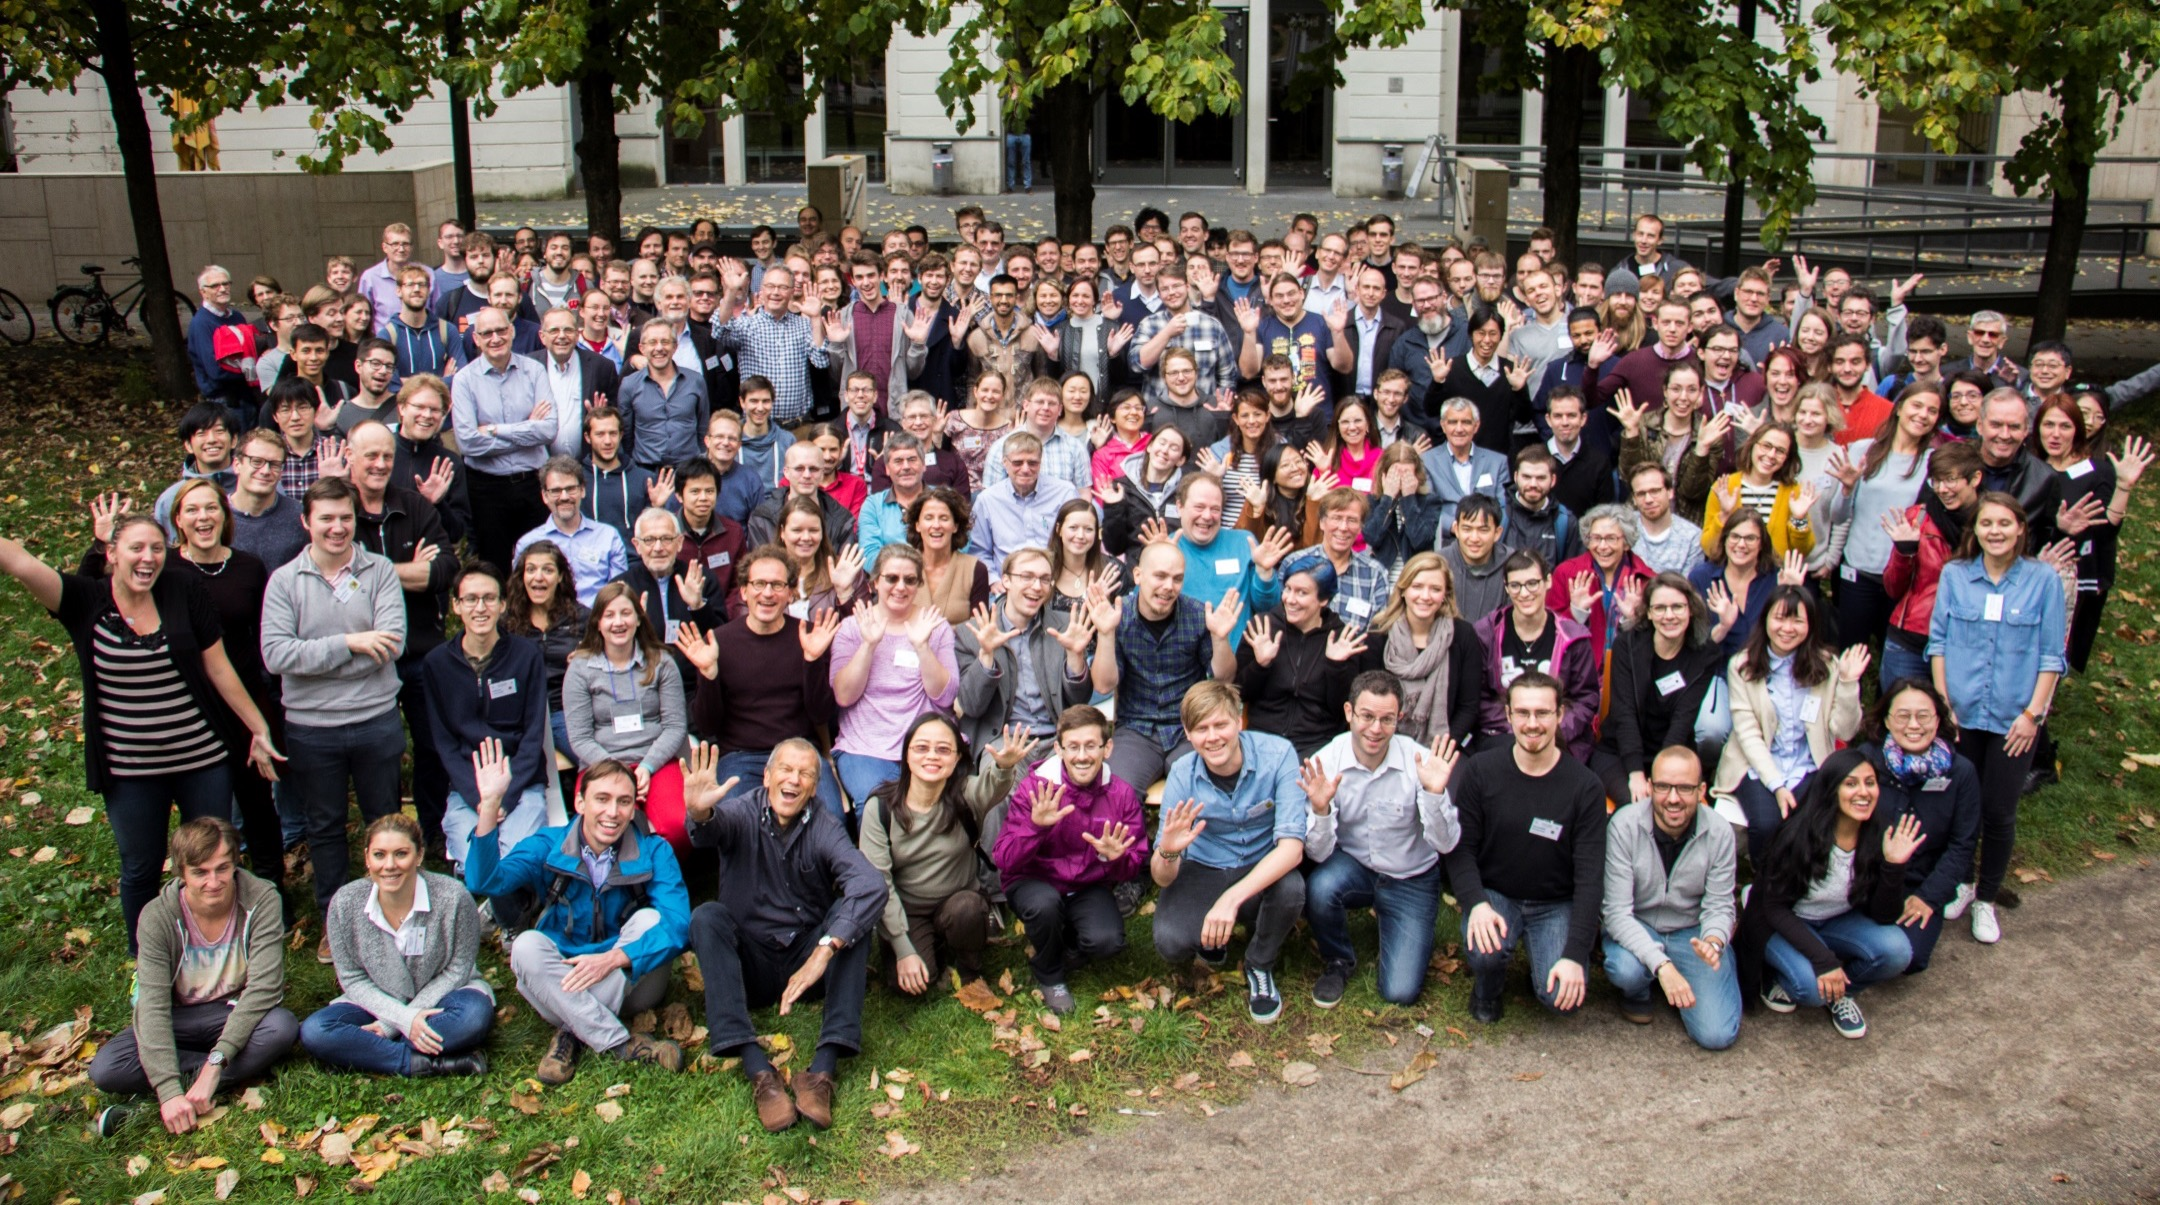
\includegraphics[width=0.94\linewidth]{halzen/icecube_colaboracion_foto.jpg}\\[1pt]
      {\scriptsize La colaboración IceCube}
    \column{0.42\textwidth}
      \small
      \begin{tcolorbox}[colback=itedaTeal, colframe=itedaTeal, arc=2pt,
        fontupper=\color{white}\small, before upper={\raggedright}]
        «Por sus contribuciones decisivas al Observatorio de Neutrinos IceCube
        y al descubrimiento de neutrinos de alta energía de origen
        astrofísico.»\\[2pt]
        {\footnotesize Real Academia Sueca de Ciencias, 6 de octubre de 2026}
      \end{tcolorbox}
      \vspace{2pt}
      {\footnotesize Impulsó el \textbf{hielo del Polo Sur} como detector
      (AMANDA, IceCube). 2013: neutrinos \textbf{astrofísicos}.}
  \end{columns}
  \credito{Foto: Colaboración IceCube, vía F.~Halzen (2024). Cita traducida de NobelPrize.org}
\end{frame}

% ---------------------------------------------------------------- 46
\begin{frame}[plain]
  \fondo[0.0]{halzen/halzen_p016_sintexto.jpg}
  \begin{tikzpicture}[remember picture, overlay]
    \node[anchor=north west, text=white, font=\Large\bfseries]
      at ([xshift=0.6cm, yshift=-0.35cm]current page.north west)
      {Otra vez Cherenkov, ahora en el hielo};
    \tikzset{rot/.style={font=\small, align=left, text=white}}
    \node[rot, anchor=west] at ([xshift=12.4cm, yshift=1.05cm]current page.south west)
      {$\nu_\mu + N \to \mu + X$\\{\footnotesize el $\nu$ no deja luz}};
    \node[rot, anchor=east] at ([xshift=8.7cm, yshift=2.6cm]current page.south west)
      {\textbf{muón}: km de traza\\emitiendo luz};
    \node[rot, anchor=east] at ([xshift=3.4cm, yshift=5.3cm]current page.south west)
      {módulos\\ópticos};
    \node[anchor=north east, fill=white, rounded corners=3pt, inner sep=2pt]
      at ([xshift=-0.4cm, yshift=-0.5cm]current page.north east)
      {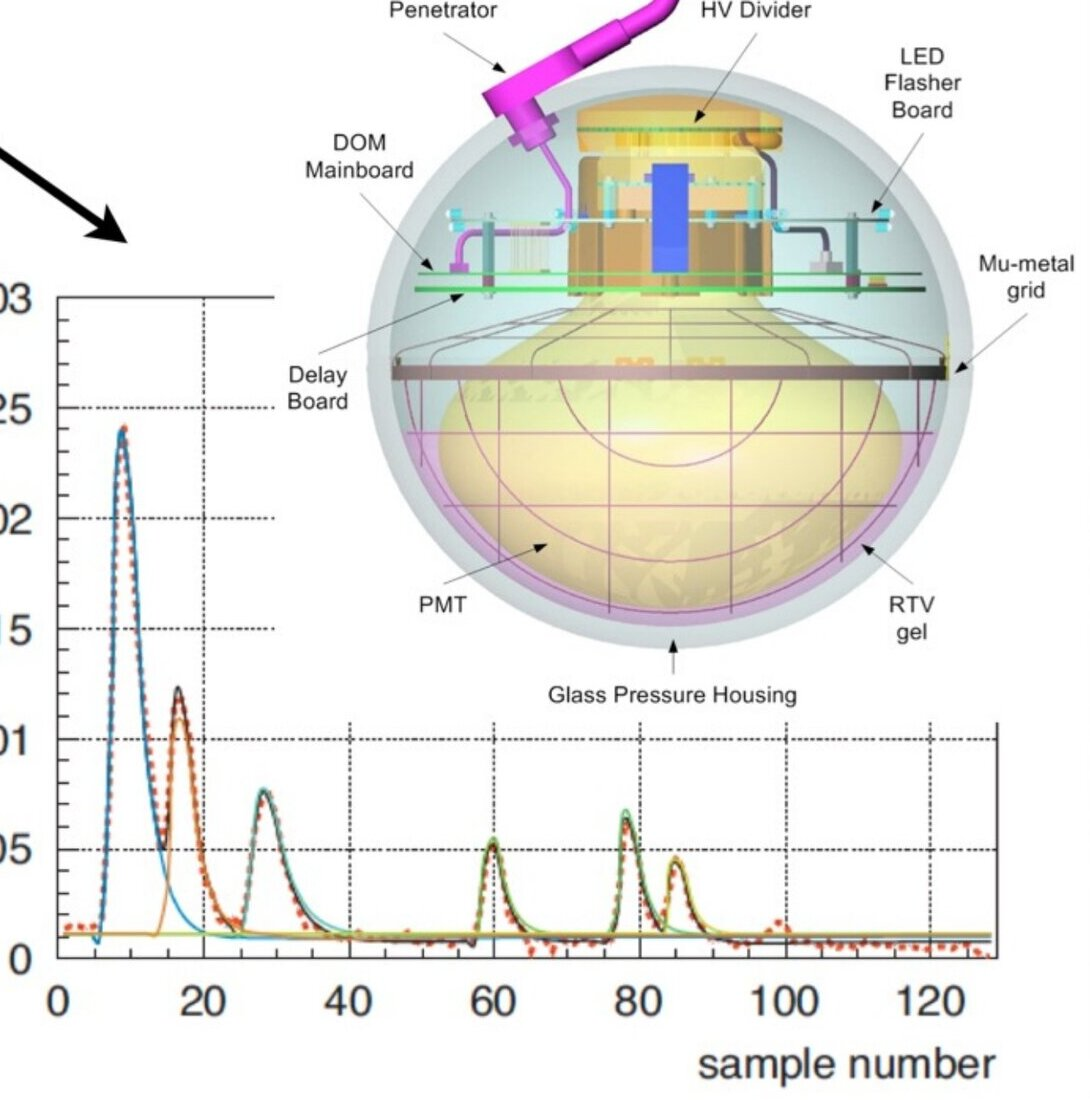
\includegraphics[height=3.4cm]{halzen/dom_formas_onda.jpg}};
    \node[anchor=north east, text width=4.9cm, align=left, text=white, font=\footnotesize]
      at ([xshift=-0.4cm, yshift=-4.1cm]current page.north east) {%
      Cada módulo \textbf{digitaliza} la forma de onda y le pone tiempo con
      precisión de nanosegundos. Con $\theta_C\approx41^\circ$ en el hielo, el
      \textbf{patrón de tiempos} da la dirección del muón.};
  \end{tikzpicture}
  \creditoblanco{Composición e inserto: F.~Halzen, Erice 2024}
\end{frame}

% ---------------------------------------------------------------- 47
\begin{frame}{Trazas y cascadas}
  \begin{columns}[T,onlytextwidth]
    \column{0.50\textwidth}
      \centering
      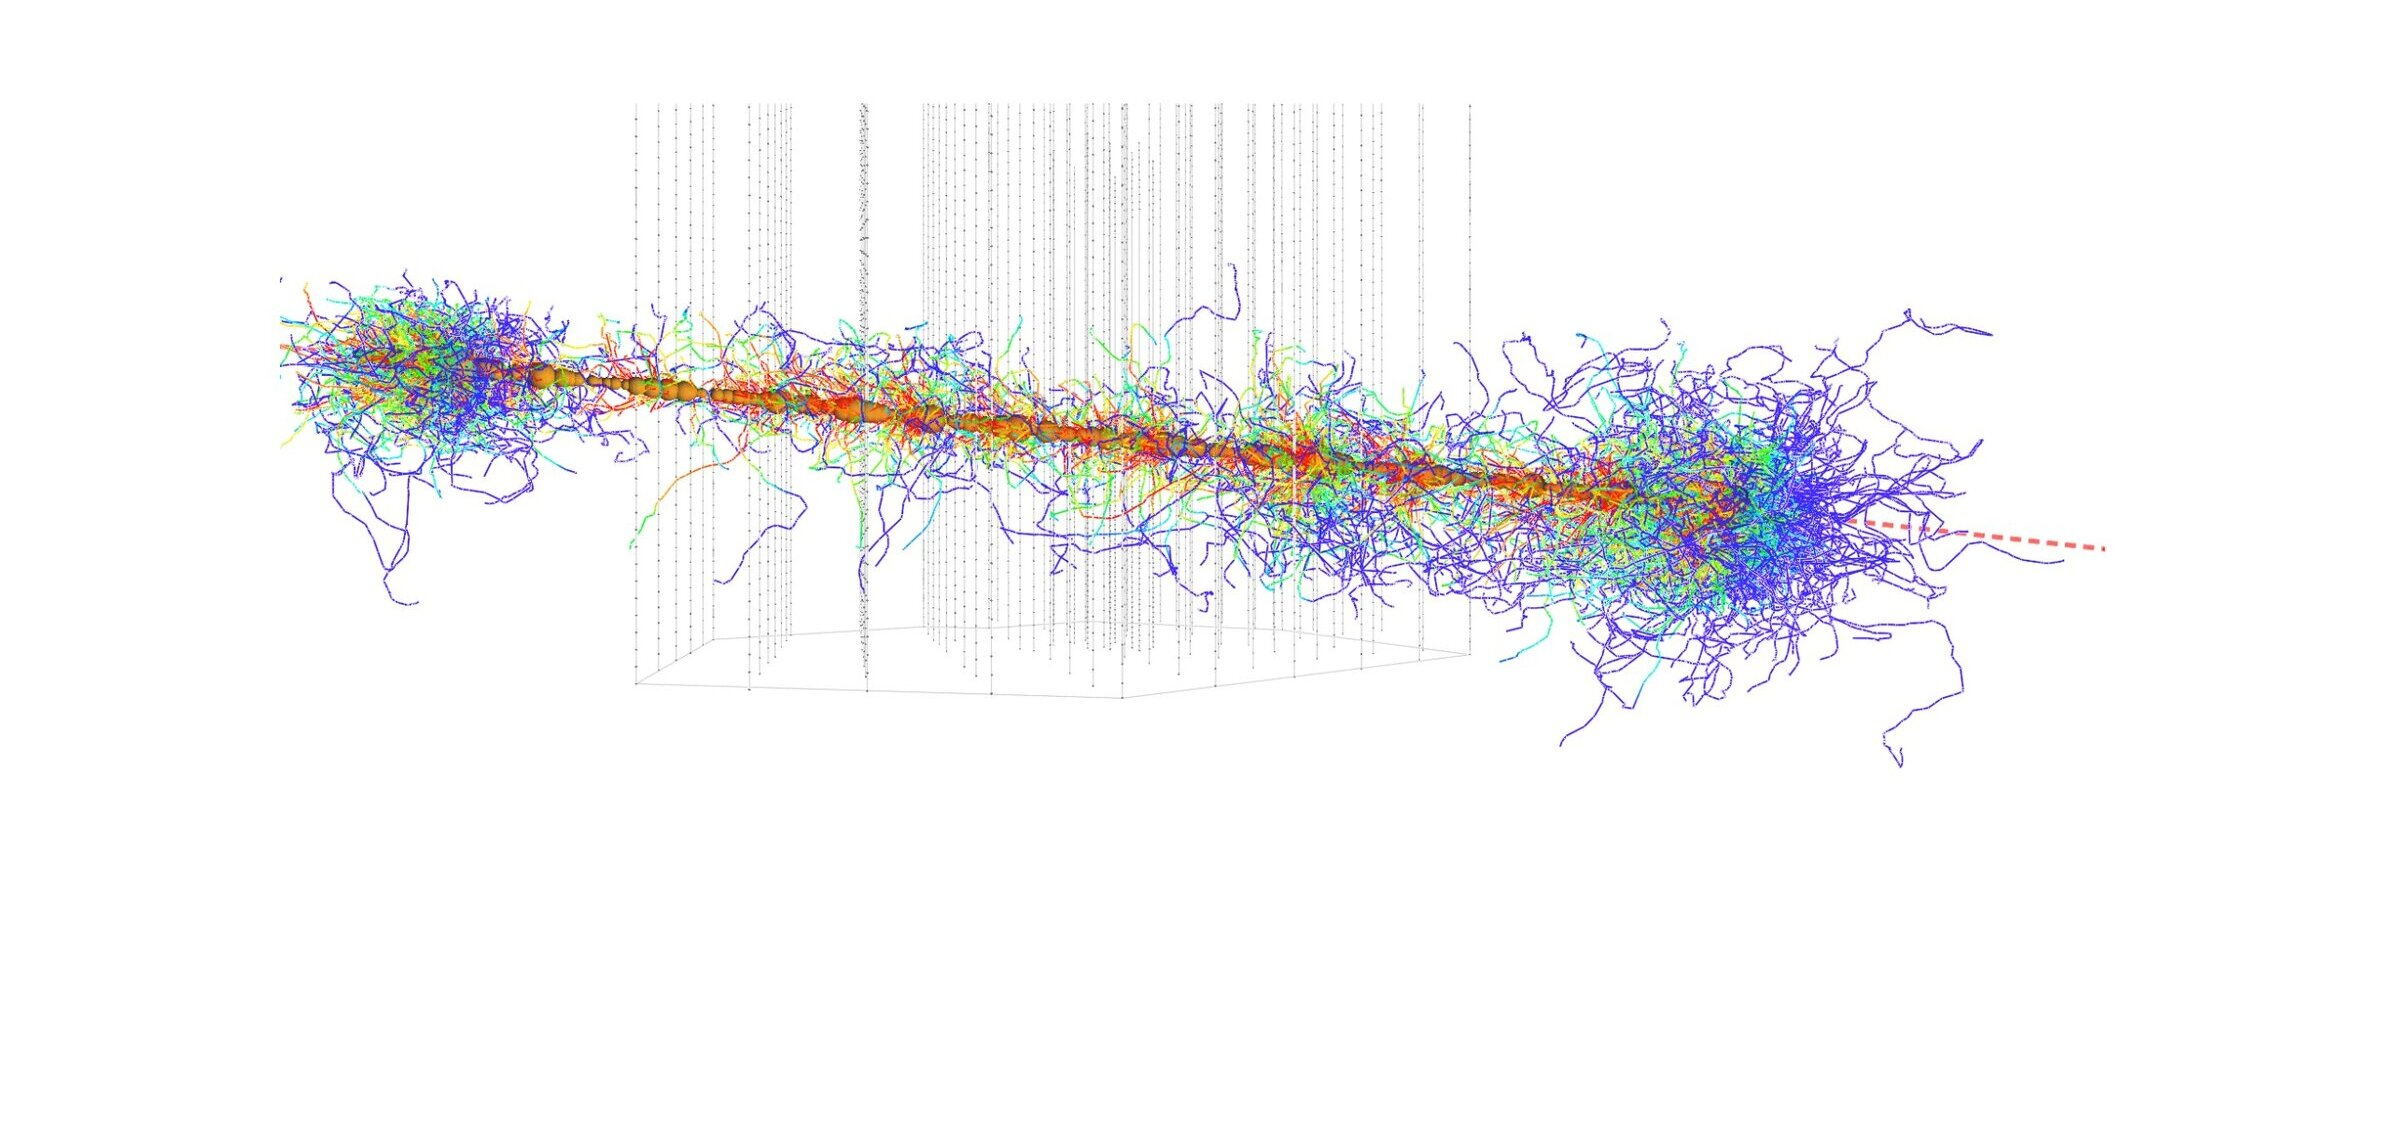
\includegraphics[height=3.0cm]{halzen/icecube_traza_r.jpg}\\[3pt]
      {\small\bfseries Traza}: $\nu_\mu$ por corriente cargada\\[2pt]
      {\footnotesize Muón de kilómetros: \textbf{dirección} con
      resolución $\lesssim1^\circ$ (hasta $\sim$0,3$^\circ$), pero sólo
      parte de la energía queda adentro.}
    \column{0.47\textwidth}
      \centering
      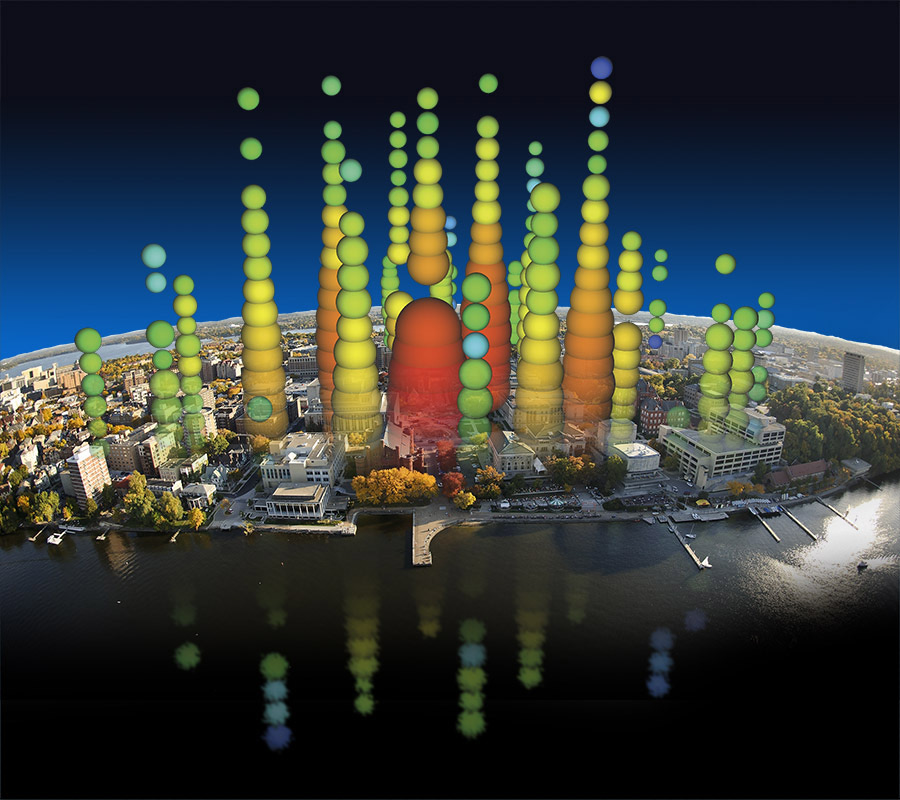
\includegraphics[height=3.0cm]{halzen/icecube_cascada_escala.jpg}\\[3pt]
      {\small\bfseries Cascada}: $\nu_e$, $\nu_\tau$ y corriente neutra\\[2pt]
      {\footnotesize Unos 10\,m de lluvia en el hielo: casi esférica vista de
      lejos. \textbf{Energía} a $\sim$10\%, dirección de $\sim$10$^\circ$.}
  \end{columns}
  \vspace{4pt}
  \begin{clave}
    Las trazas \textbf{apuntan}; las cascadas \textbf{miden energía}.
  \end{clave}
  \credito{Eventos de IceCube, vía F.~Halzen (2024). Derecha: cascada de PeV junto a edificios, para dar escala}
\end{frame}

% ---------------------------------------------------------------- 48
\begin{frame}{Una década de descubrimientos}
  \begin{columns}[T,onlytextwidth]
    \column{0.24\textwidth}
      \centering
      {\footnotesize\bfseries 2013 · flujo difuso}\\[2pt]
      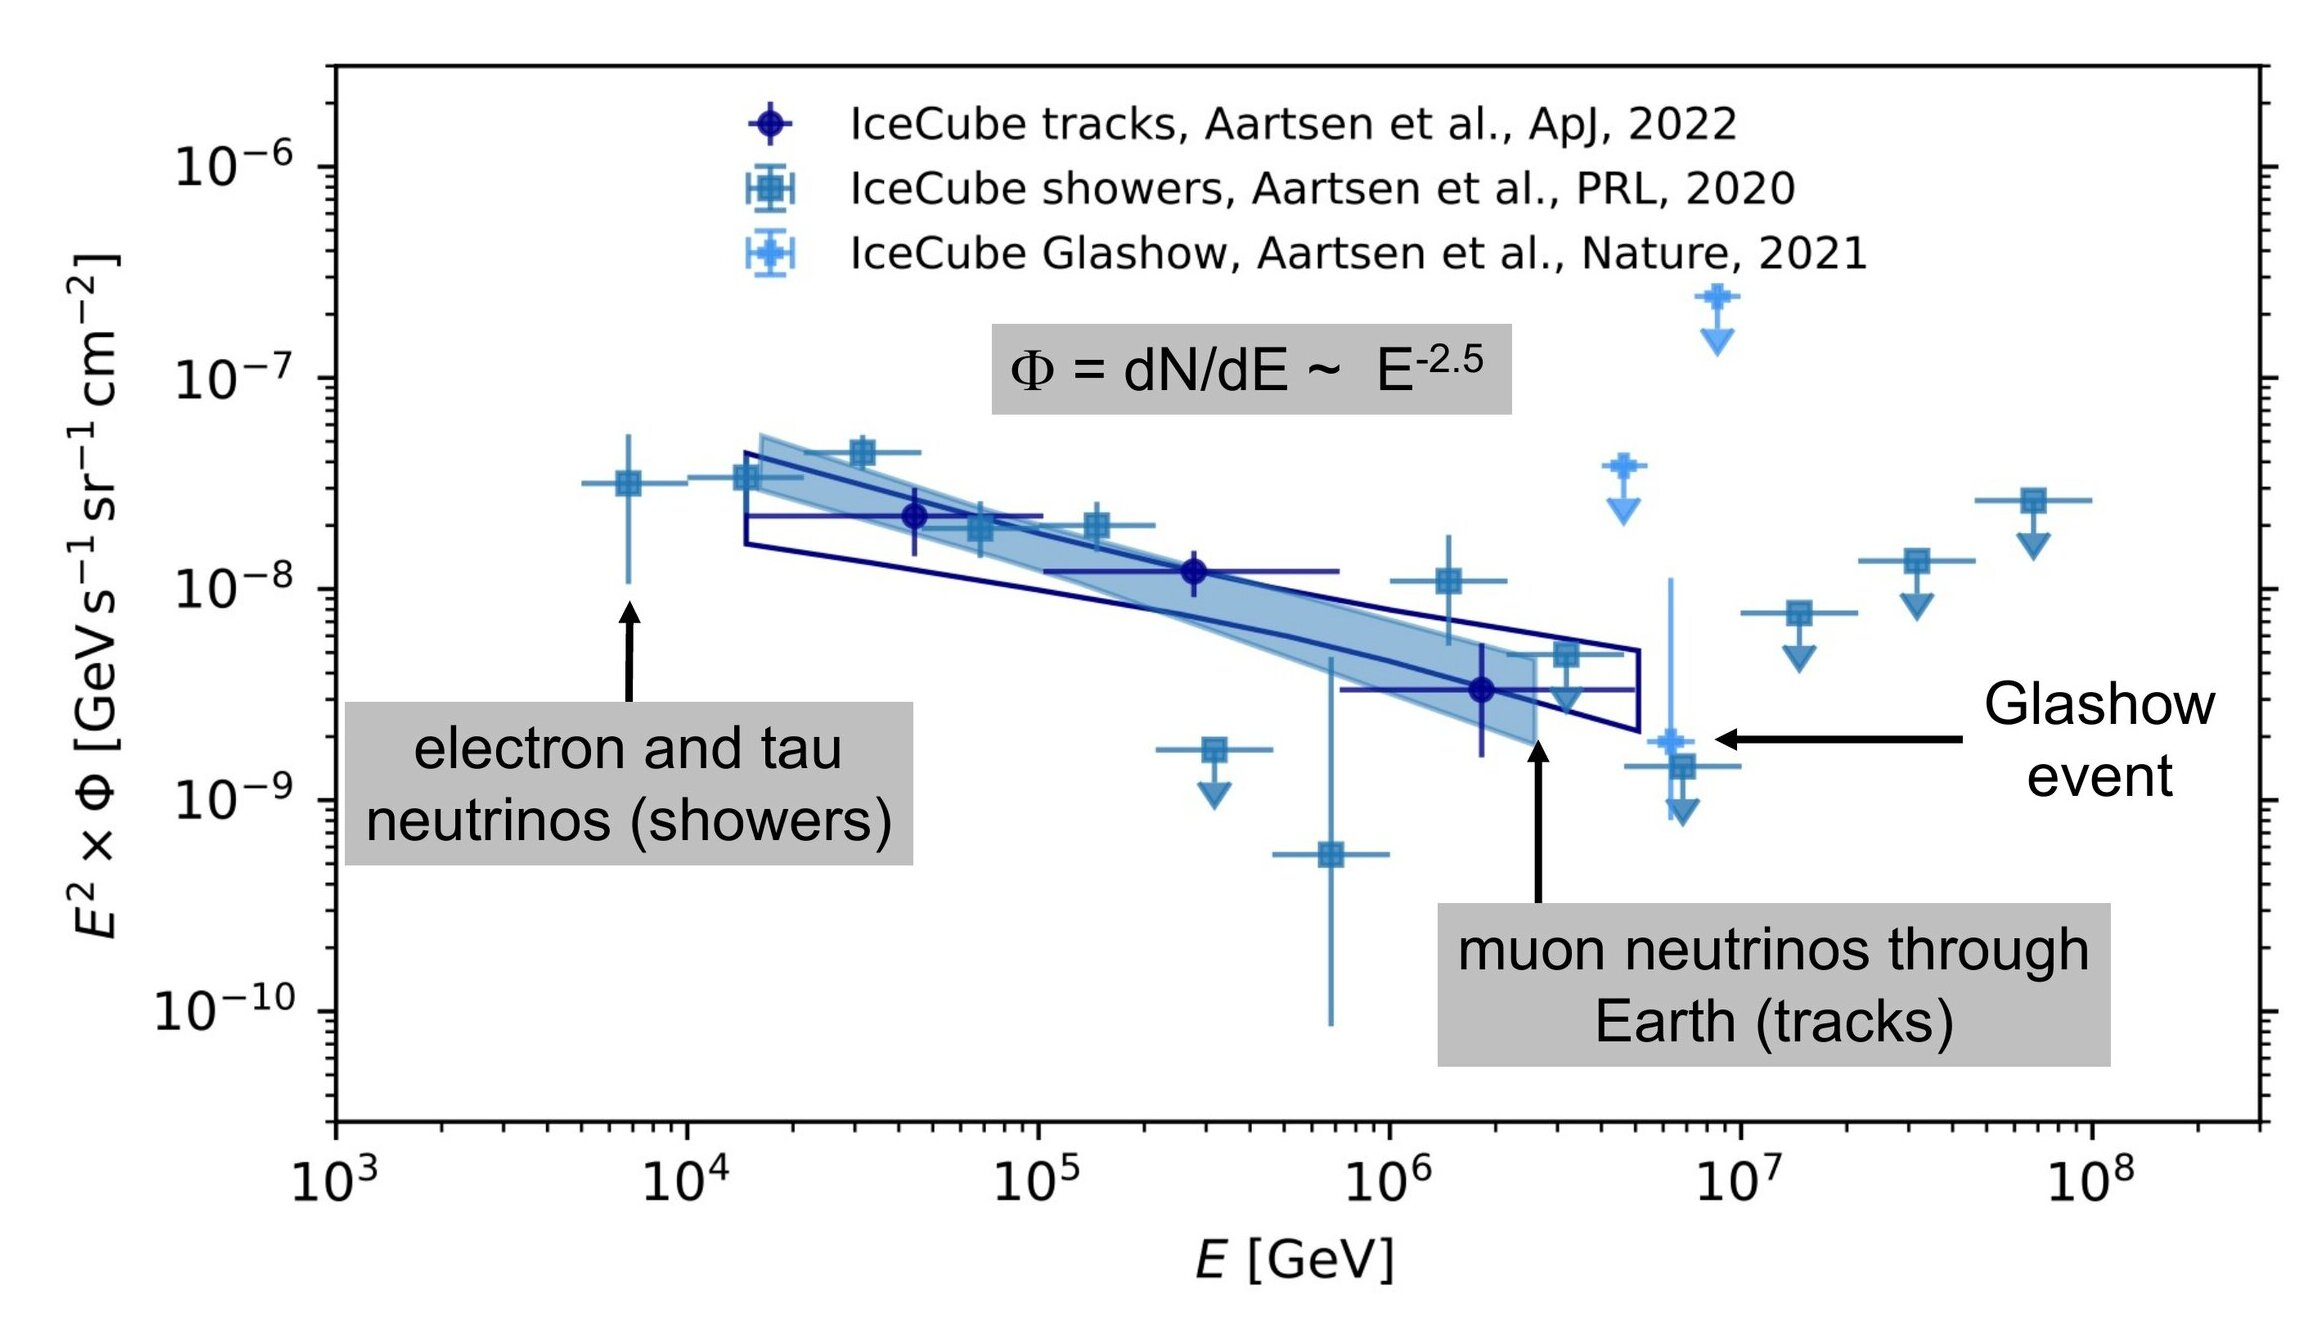
\includegraphics[width=\linewidth]{halzen/flujo_difuso.jpg}\\[2pt]
      {\scriptsize Neutrinos de TeV--PeV de origen \textbf{astrofísico}, espectro
      $\sim E^{-2,5}$.}
    \column{0.24\textwidth}
      \centering
      {\footnotesize\bfseries 2017 · TXS 0506+056}\\[2pt]
      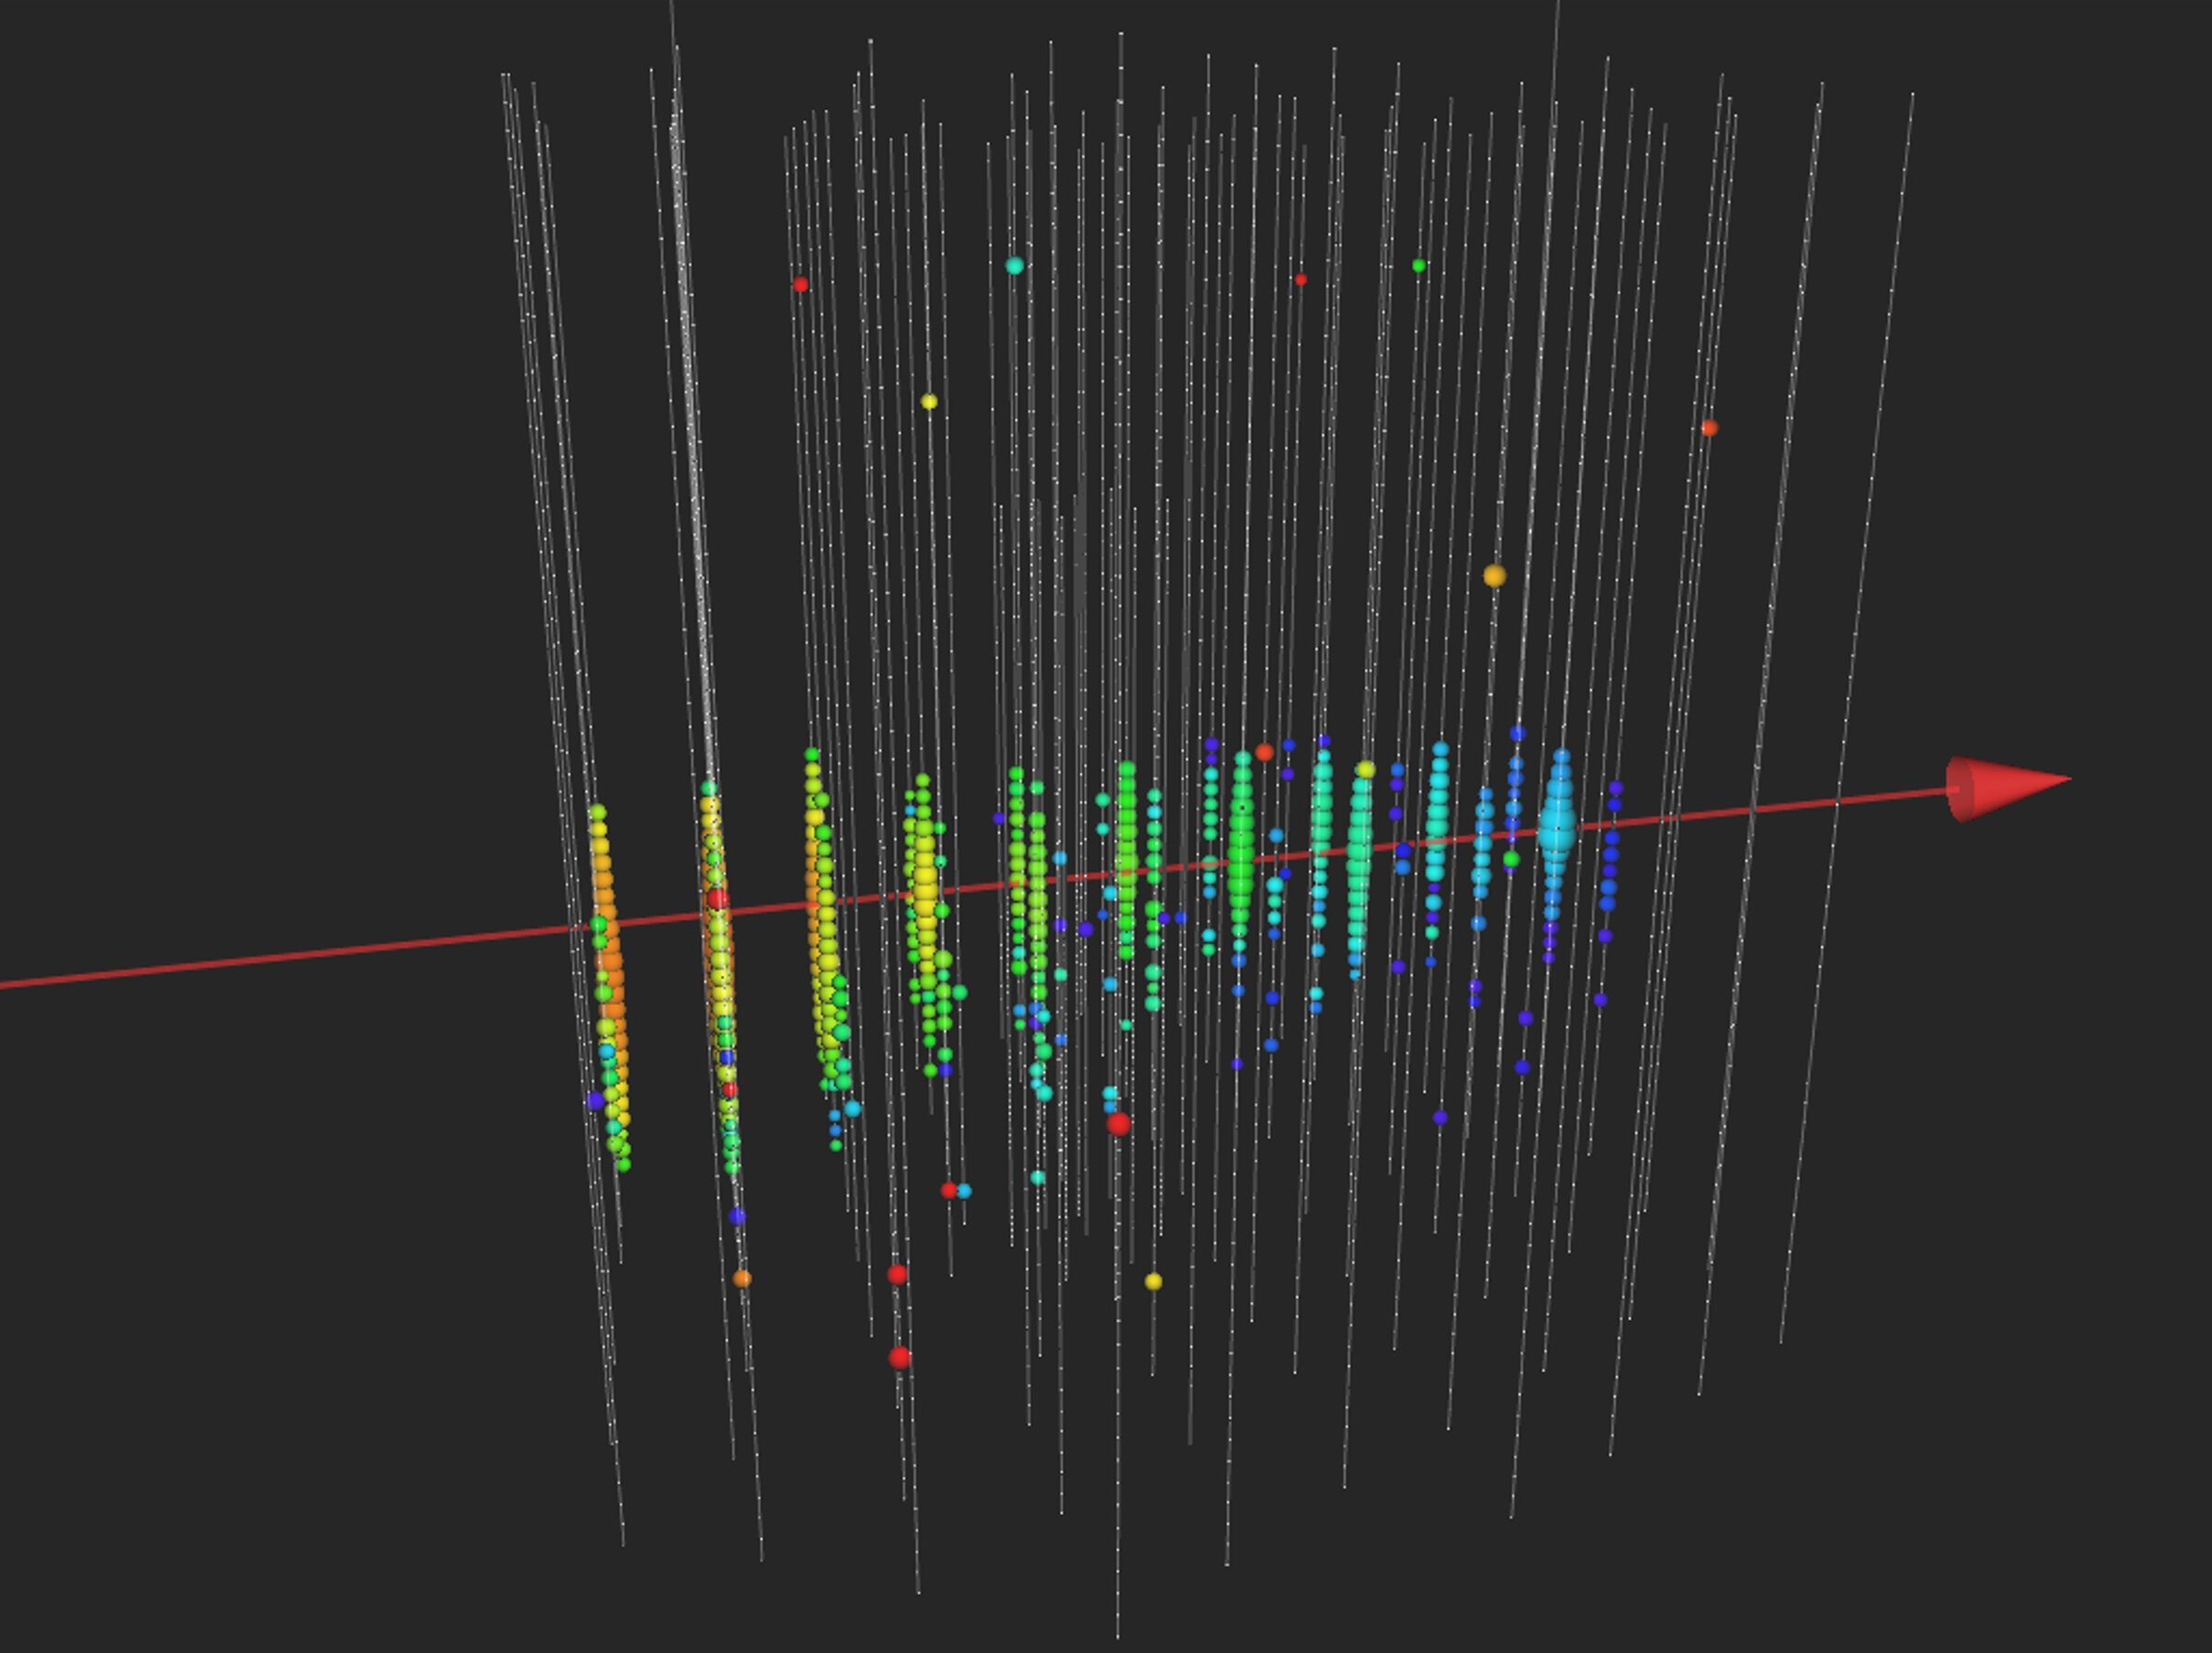
\includegraphics[width=\linewidth]{halzen/icecube_ic170922a.jpg}\\[2pt]
      {\scriptsize Un neutrino de $\sim$290\,TeV coincide con un blazar en
      \textbf{erupción gamma}.}
    \column{0.24\textwidth}
      \centering
      {\footnotesize\bfseries 2022 · NGC 1068}\\[2pt]
      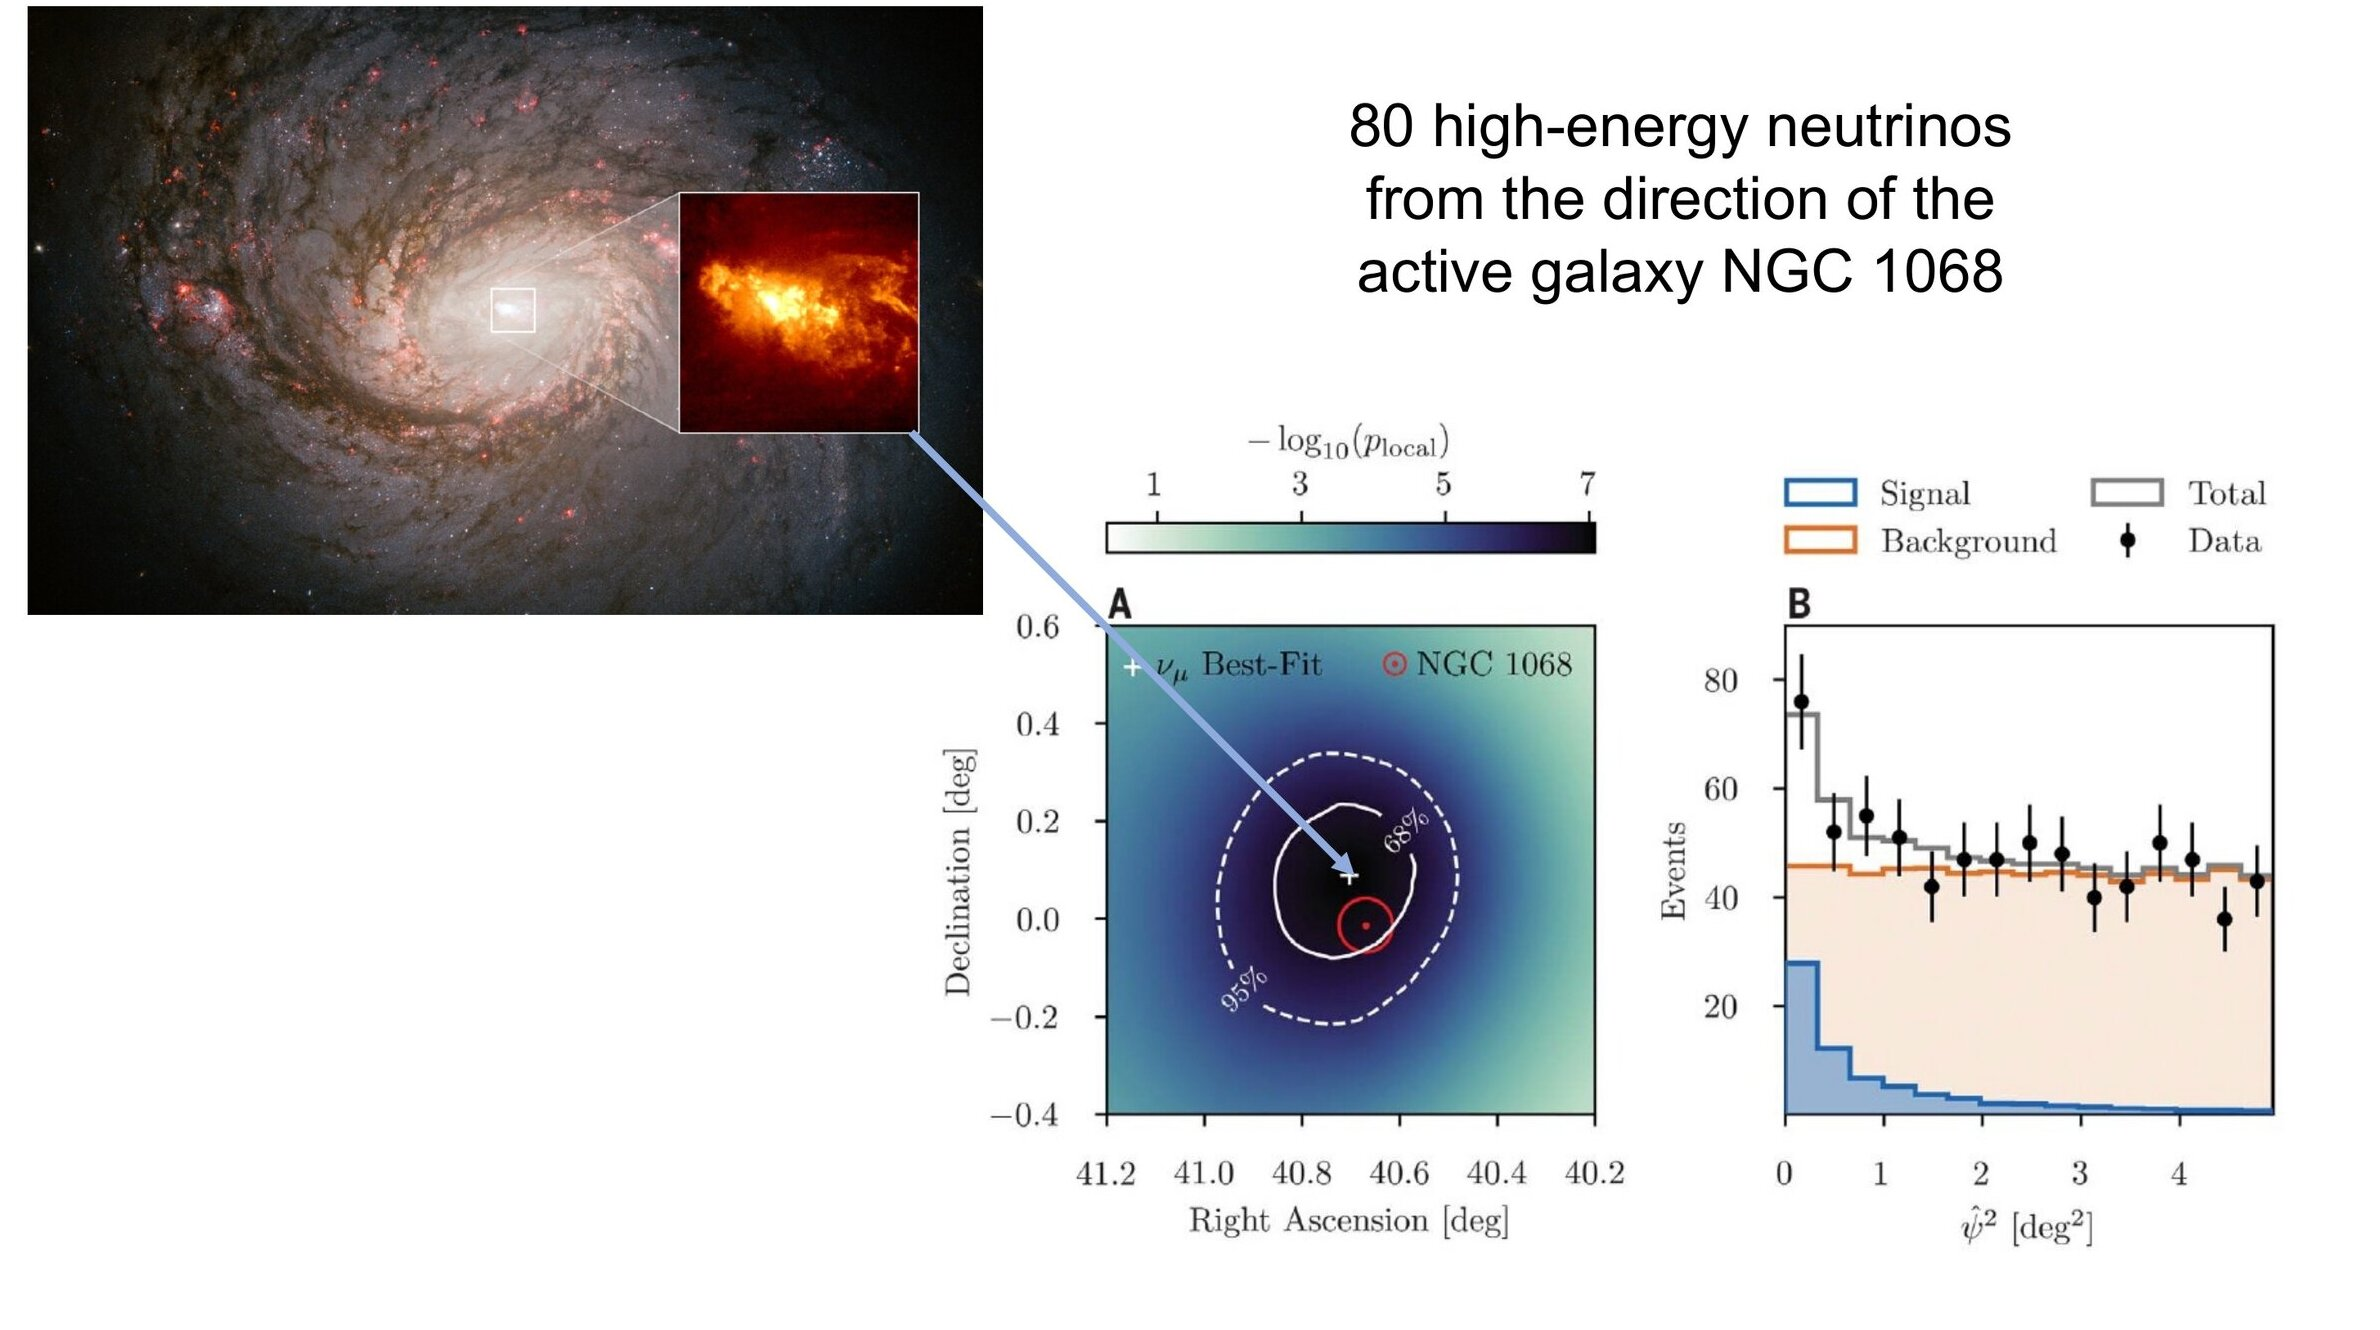
\includegraphics[width=\linewidth]{halzen/ngc1068.jpg}\\[2pt]
      {\scriptsize $\sim$80 neutrinos de una galaxia activa cercana, a
      4,2$\sigma$, \textbf{sin} gammas de TeV: núcleo opaco.}
    \column{0.24\textwidth}
      \centering
      {\footnotesize\bfseries 2023 · nuestra galaxia}\\[2pt]
      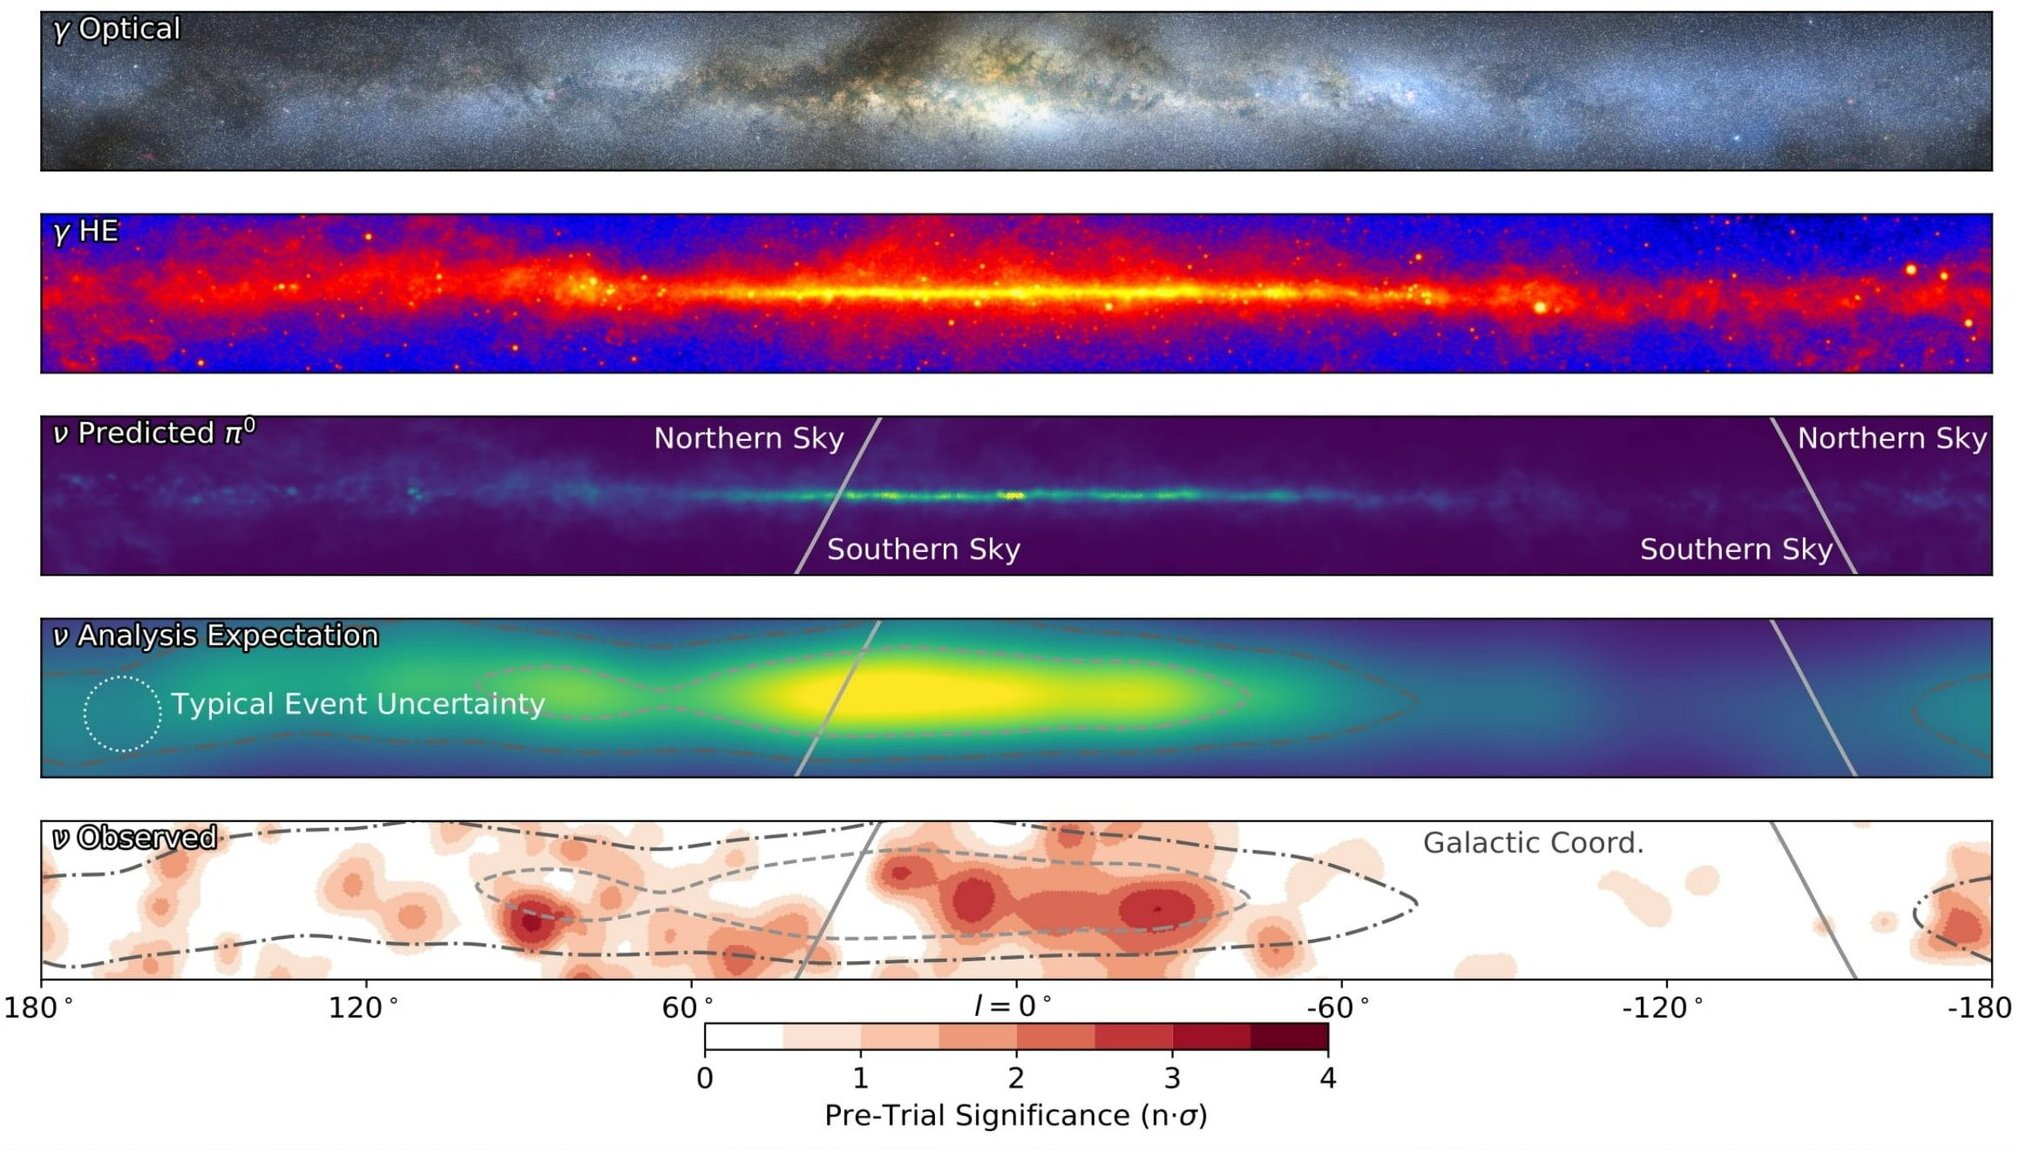
\includegraphics[width=\linewidth]{halzen/plano_galactico_fermi_icecube.jpg}\\[2pt]
      {\scriptsize El plano galáctico en neutrinos (4,5$\sigma$), como lo predicen
      los rayos cósmicos sobre el gas.}
  \end{columns}
  \vspace{6pt}
  \begin{clave}
    La fuente de neutrinos más clara no es la más brillante en gammas: los
    neutrinos ven \textbf{adentro} de los aceleradores.
  \end{clave}
  \credito{Figuras: Colaboración IceCube (Science 2013, 2018, 2022, 2023), vía F.~Halzen (2024)}
\end{frame}

% ---------------------------------------------------------------- 48b
\begin{frame}{NGC 1068: neutrinos desde el corazón de una galaxia activa}
  \begin{columns}[c,onlytextwidth]
    \column{0.55\textwidth}
      \centering
      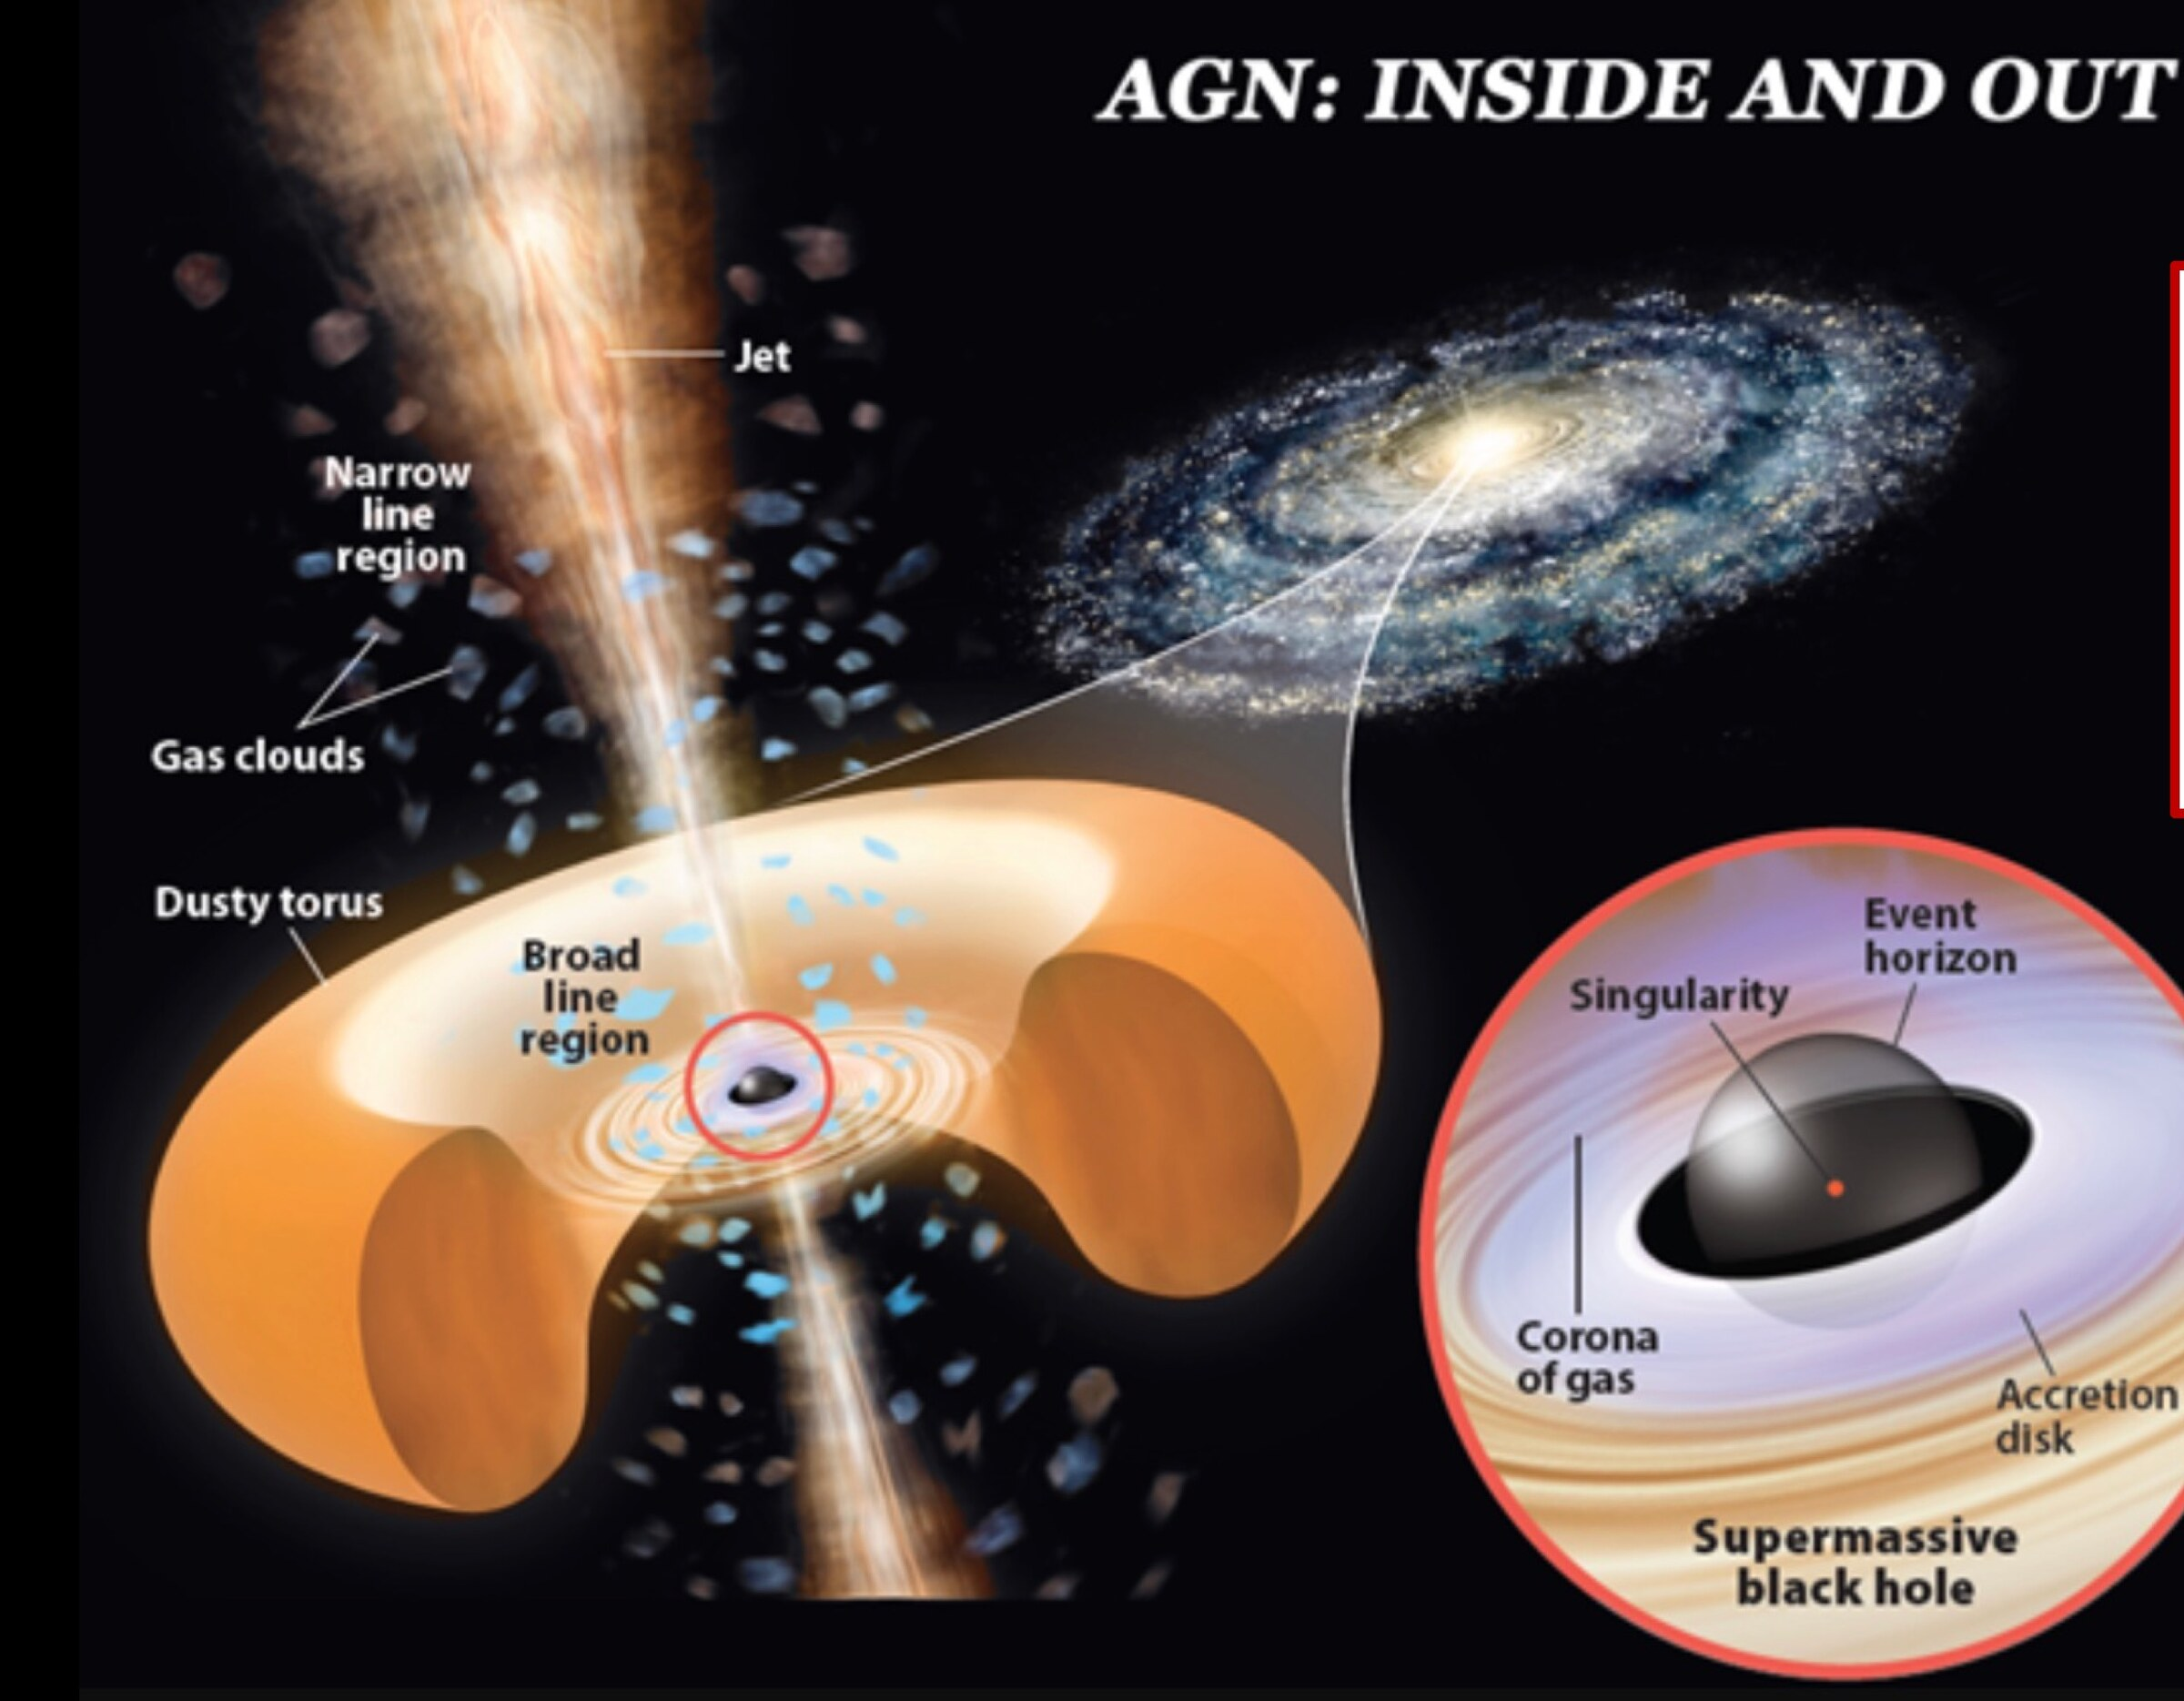
\includegraphics[width=\linewidth]{halzen/agn_inside_out.jpg}
    \column{0.42\textwidth}
      \footnotesize
      Un \textbf{núcleo galáctico activo} (AGN): un agujero negro gigante que
      traga gas de un disco, rodeado por una \textbf{corona} caliente que
      brilla en rayos X.
      \vspace{2pt}
      \begin{itemize}\footnotesize
        \item IceCube vio $\sim$80 neutrinos de 1,5--15\,TeV desde NGC 1068
          (a $\sim$14\,Mpc), con 4,2$\sigma$.
        \item Pero \textbf{no llegan los gammas} que deberían acompañarlos.
      \end{itemize}
      \begin{clave}[fontupper=\footnotesize]
        Los gammas chocan con los rayos X de la corona y quedan atrapados; los
        neutrinos escapan. Se producen \textbf{muy cerca del agujero negro},
        donde la luz no sale.
      \end{clave}
  \end{columns}
  \creditoizq{Ilustración: «AGN: inside and out», vía F.~Halzen (2024). IceCube, Science 378 (2022) 538}
\end{frame}

% ---------------------------------------------------------------- 48c
\begin{frame}{La Vía Láctea vista con neutrinos}
  \begin{columns}[c,onlytextwidth]
    \column{0.55\textwidth}
      \centering
      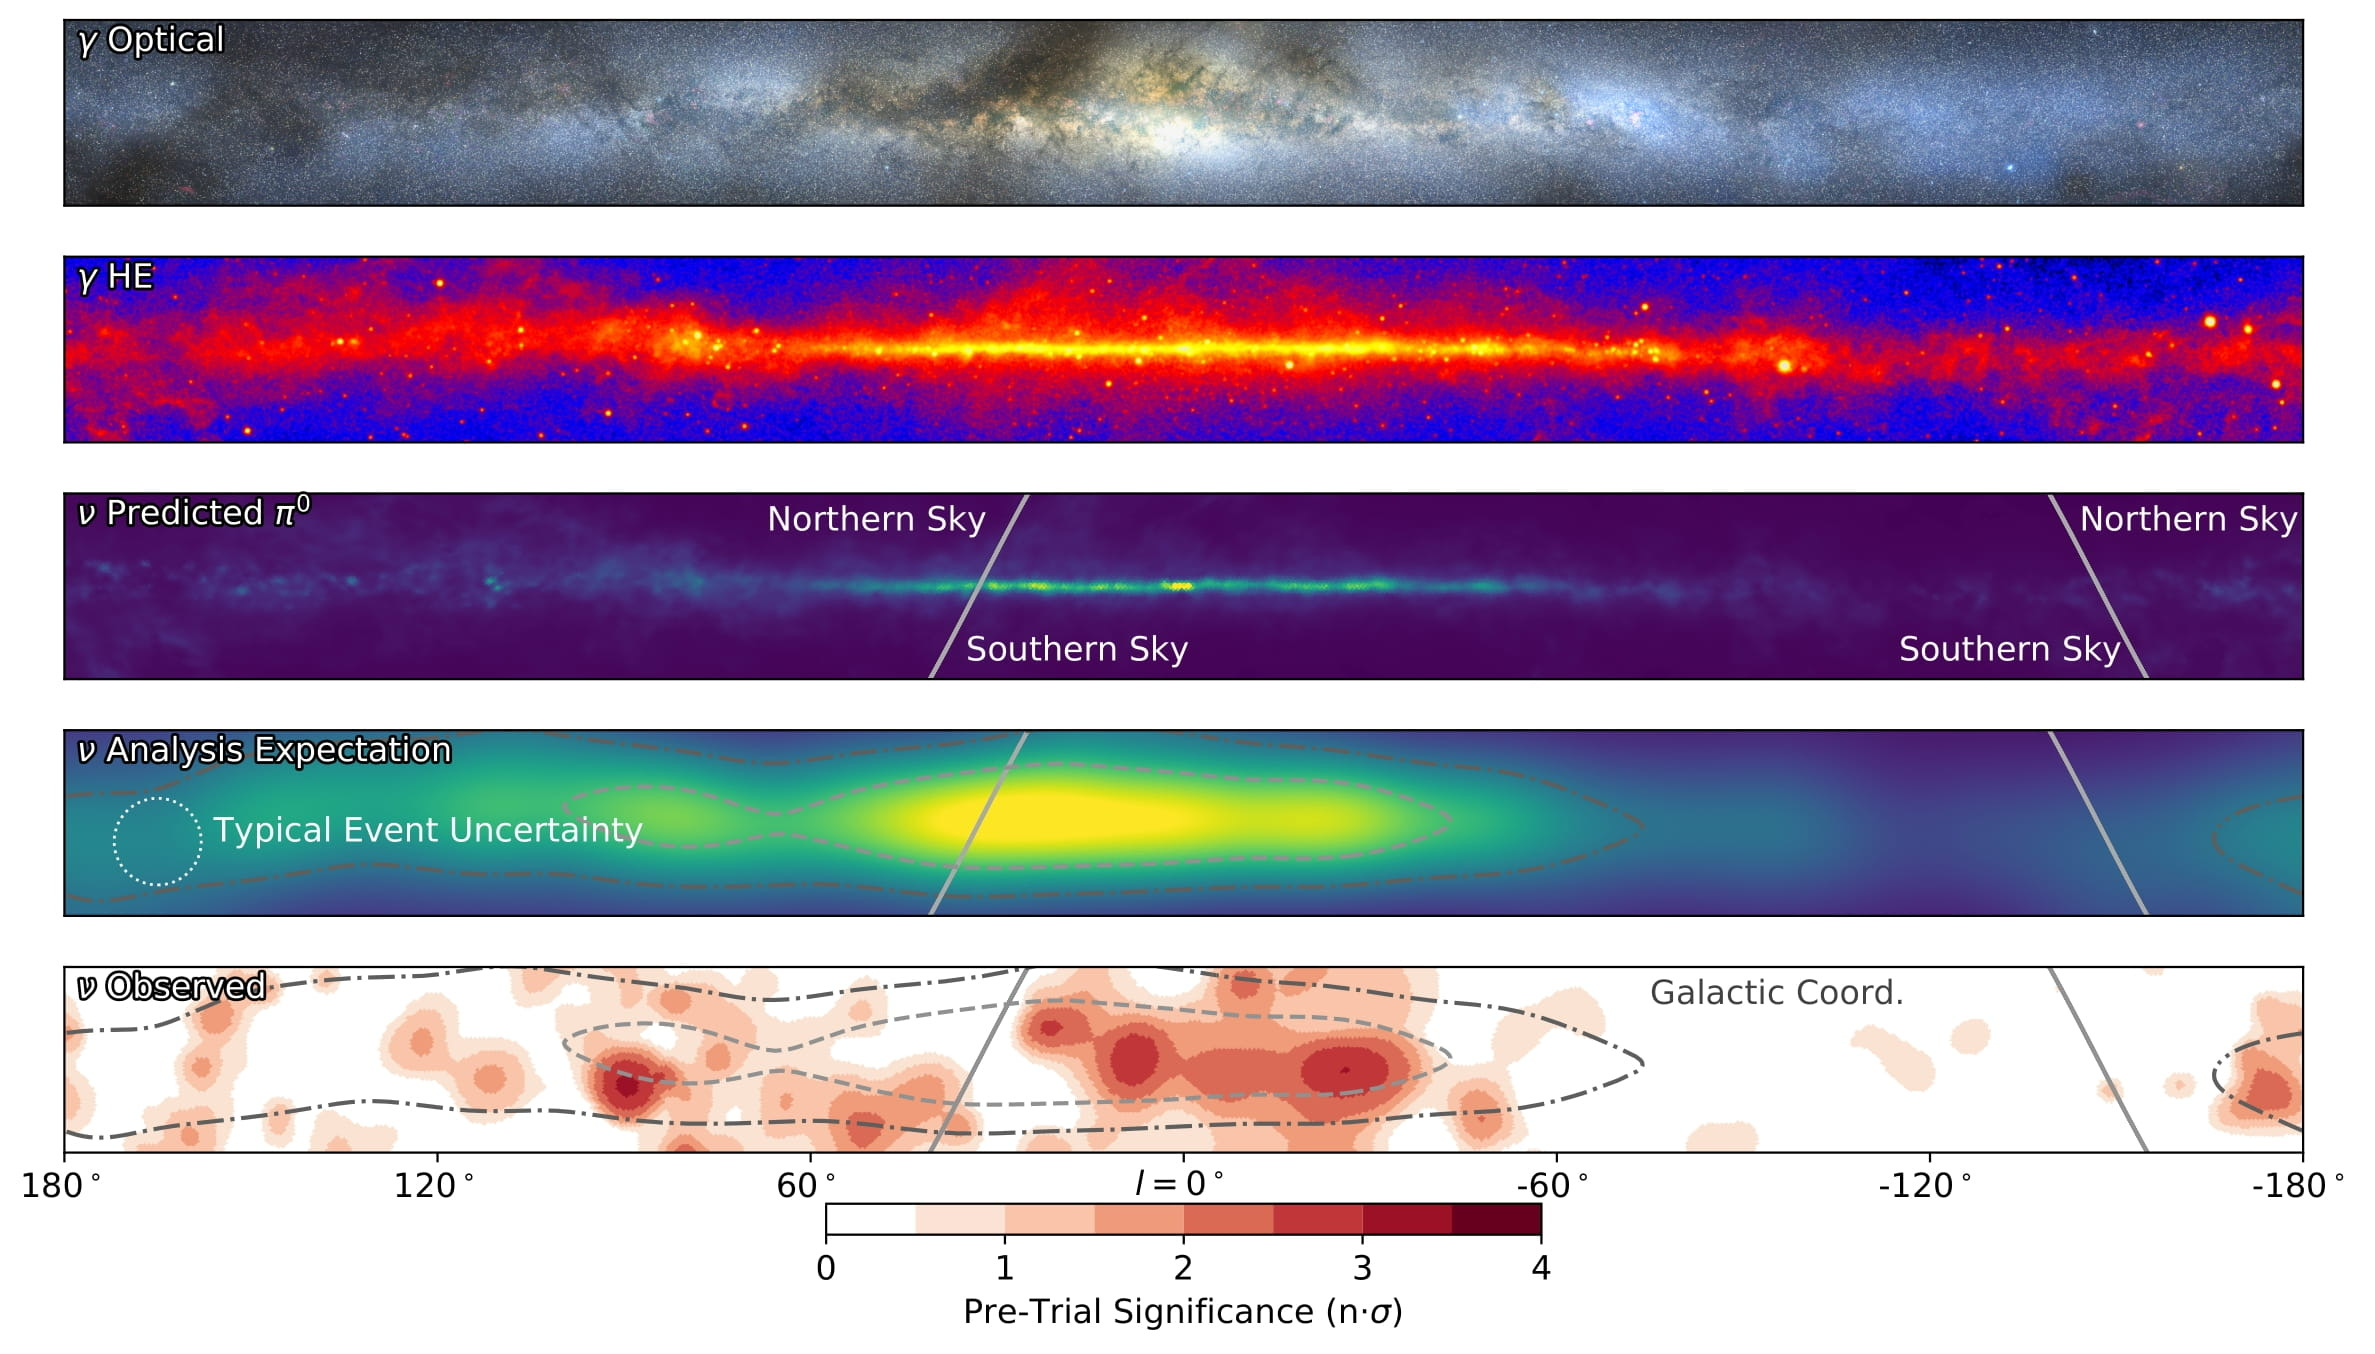
\includegraphics[width=\linewidth]{halzen/plano_galactico_paneles.jpg}
    \column{0.42\textwidth}
      \footnotesize
      De arriba a abajo: el plano de la galaxia en \textbf{luz visible}, en
      \textbf{rayos gamma} (Fermi), la \textbf{predicción} de neutrinos y lo
      que \textbf{observó} IceCube.
      \vspace{2pt}
      \begin{itemize}\footnotesize
        \item Los rayos cósmicos de la galaxia chocan con el gas interestelar:
          producen piones, que dan gammas \emph{y} neutrinos.
        \item IceCube encontró esa emisión a lo largo del plano (no sólo del
          centro), con 4,5$\sigma$ (2023).
      \end{itemize}
      \begin{clave}[fontupper=\footnotesize]
        La primera imagen de nuestra galaxia en neutrinos, como predicen los
        rayos cósmicos.
      \end{clave}
  \end{columns}
  \creditoizq{IceCube, Science 380 (2023) 1338, vía F.~Halzen (2024)}
\end{frame}

% ---------------------------------------------------------------- 49
\begin{frame}{Auger e IceCube: dos instrumentos, dos problemas}
  \begin{tikzpicture}[x=1cm,y=1cm]
    \tikzset{
      cab/.style={font=\small\bfseries, text=white, minimum width=5.6cm,
        minimum height=0.6cm, rounded corners=2pt},
      fila/.style={font=\footnotesize, text width=5.2cm, align=left, anchor=north west},
      lab/.style={font=\scriptsize\bfseries, text=itedaGray, anchor=north east, align=right}}
    \node[cab, fill=itedaOrange] at (5.2,0) {Pierre Auger};
    \node[cab, fill=cmbAzul] at (11.1,0) {IceCube};
    \foreach \y/\l/\a/\b in {
        -0.5/{Geometría}/{Superficie de 3000\,km$^2$}/{Volumen de 1\,km$^3$},
        -1.15/{Qué detecta}/{Lluvias de rayos cósmicos}/{Secundarios de interacciones de $\nu$},
        -1.8/{Cherenkov}/{Agua: \textbf{muestrea} la lluvia}/{Hielo: \textbf{blanco y calorímetro}},
        -2.45/{Energías}/{$\gtrsim10^{17}$\,eV}/{$10^{10}$ a $10^{16}$\,eV (10\,GeV a 10\,PeV)},
        -3.1/{Fortaleza}/{Exposición a lo más raro}/{Direcciones y sabores de $\nu$}}{
      \node[lab] at (2.35,\y) {\l};
      \node[fila] at (2.55,\y) {\a};
      \node[fila] at (8.45,\y) {\b};
      \draw[itedaGray!30] (0.4,\y+0.08) -- (13.9,\y+0.08);}
  \end{tikzpicture}\\[2pt]
  {\footnotesize\color{itedaGray} Auger también busca $\nu$ muy inclinados;
  IceCube también registra muones atmosféricos y lluvias (IceTop).}\\[2pt]
  {\scriptsize\color{itedaTealDark}\textbf{Prefijos:} G (giga) $=10^9$ \quad T (tera) $=10^{12}$
  \quad P (peta) $=10^{15}$ \quad E (exa) $=10^{18}$}\\[3pt]
  \begin{clave}
    La aceptación de cada uno sale de su \textbf{blanco} (atmósfera o hielo)
    y de su \textbf{umbral}: a 1\,PeV, un neutrino interactúa en 1\,km de hielo
    con probabilidad $\sim5\times10^{-5}$.
  \end{clave}
\end{frame}

% ---------------------------------------------------------------- 50
\begin{frame}{Astronomía multimensajero}
  \begin{columns}[c,onlytextwidth]
    \column{0.47\textwidth}
      \centering
      \begin{tikzpicture}[x=1cm,y=1cm]
        \shade[ball color=black!80] (0,0) circle (0.35);
        \fill[itedaOrange!60] (-0.1,0.3) -- (0.1,0.3) -- (0.35,2.0) -- (-0.35,2.0) -- cycle;
        \node[font=\scriptsize, text=itedaGray] at (0,-0.6) {fuente};
        \draw[very thick, itedaOrange, -{Stealth}] (0.4,0.1) .. controls (1.5,1.6) and (2.2,-1.3) .. (4.0,0.9);
        \node[font=\scriptsize, text=itedaOrange, anchor=west, align=left] at (4.05,0.9) {rayos\\cósmicos};
        \draw[very thick, cmbAzul, -{Stealth}] (0.4,-0.2) -- (2.8,-0.45);
        \node[font=\scriptsize, text=cmbAzul] at (3.0,-0.47) {$\times$};
        \node[font=\scriptsize, text=cmbAzul, anchor=west] at (3.2,-0.47) {fotones};
        \draw[very thick, violetaNu, -{Stealth}] (0.4,-0.45) -- (4.0,-1.2);
        \node[font=\scriptsize, text=violetaNu, anchor=west] at (4.05,-1.2) {neutrinos};
        \draw[very thick, verdeRadio, -{Stealth}, decorate, decoration={snake, amplitude=1mm,
          segment length=4mm, post length=2mm}] (0.4,-0.7) -- (4.0,-1.95);
        \node[font=\scriptsize, text=verdeRadio, anchor=west, align=left] at (4.05,-1.95) {ondas\\gravitac.};
      \end{tikzpicture}\\[4pt]
      {\footnotesize Cada mensajero interactúa distinto \textbf{en la fuente} y
      \textbf{en el camino}: juntos reconstruyen el acelerador.}
    \column{0.50\textwidth}
      \small
      \textbf{GW170817}: dos estrellas de neutrones a $\sim$40\,Mpc.
      \vspace{2pt}

      \begin{tikzpicture}[x=1cm,y=1cm]
        \draw[itedaGray, thick] (0,0) -- (0,-3.6);
        \foreach \y/\t/\d in {0/{$t_0$}/{ondas gravitacionales (LIGO--Virgo)},
          -0.9/{+1,7\,s}/{estallido de rayos gamma (Fermi, INTEGRAL)},
          -1.8/{+11\,h}/{kilonova óptica en NGC 4993},
          -2.7/{+9\,d}/{rayos X},
          -3.6/{+16\,d}/{radio}}{
          \fill[itedaOrange] (0,\y) circle (2.2pt);
          \node[font=\scriptsize\bfseries, anchor=east] at (-0.15,\y) {\t};
          \node[font=\scriptsize, anchor=west] at (0.15,\y) {\d};}
      \end{tikzpicture}\\[4pt]
      {\footnotesize IceCube, ANTARES y \textbf{Auger} buscaron neutrinos:
      ninguno, compatible con un chorro visto de costado.}
  \end{columns}
  \credito{LIGO--Virgo \textit{et al.}, ApJL 848 (2017) L12; ANTARES, IceCube y Auger, ApJL 850 (2017) L35}
\end{frame}

% ======================================================================
% BLOQUE 6 — HERON y cierre
% ======================================================================
\section{HERON y cierre}
\bloque{NEUTRINOS}

% ---------------------------------------------------------------- 50
\begin{frame}{El problema de la ultra alta energía: contar lo que casi no llega}
  \begin{columns}[c,onlytextwidth]
    \column{0.50\textwidth}
      \small
      \[ N_\nu = T\!\int\! dE\;\Phi_\nu(E)\,\big[A\Omega\big]_\mathrm{ef}(E) \]
      \vspace{-4pt}
      \begin{itemize}\footnotesize
        \item \textbf{Sección eficaz} $\sigma_{\nu N}(E)$: propiedad del neutrino.
        \item \textbf{Probabilidad de interacción} $P\simeq n\,\sigma\,L$ en un
          espesor $L$.
        \item \textbf{Volumen efectivo}: donde una interacción \emph{se detecta}.
        \item \textbf{Aceptación} $[A\Omega]_\mathrm{ef}$ (km$^2$\,sr) y
          \textbf{exposición} (km$^2$\,sr\,año): lo que el detector
          realmente integra.
      \end{itemize}
    \column{0.47\textwidth}
      \begin{clave}
        A EeV los flujos esperados son tan bajos que se necesitan
        \textbf{cientos de km$^3$} efectivos.
      \end{clave}
      \vspace{3pt}
      {\footnotesize
      \textbf{Óptico}: la luz se absorbe en $\sim$100\,m: sensores cada
      $\sim$100\,m. 1\,km$^3$ son 5160 sensores; 100\,km$^3$ serían cientos de
      miles.\\[3pt]
      \textbf{Radio}: atraviesa km de hielo y decenas de km de aire. Pocas
      antenas cubren volúmenes enormes, con umbral más alto.}\\[5pt]
      {\footnotesize\color{itedaGray} El régimen existe: KM3NeT detectó un
      neutrino de $\sim$220\,PeV (KM3-230213A, \textit{Nature} 2025).}
  \end{columns}
\end{frame}

% ---------------------------------------------------------------- 51
\bloque{}
\begin{frame}[plain]
  \fondo[0.25]{externas/ischigualasto_valle.jpg}
  \velo[0.9]{l}
  \begin{tikzpicture}[remember picture, overlay]
    \node[anchor=west, text=white, align=left, text width=10cm]
      at ([xshift=0.8cm, yshift=0.3cm]current page.west) {%
      {\small\color{itedaOrange}\bfseries EL PRÓXIMO GRAN OBSERVATORIO\\DE NEUTRINOS, EN ARGENTINA}\\[8pt]
      {\fontsize{44}{48}\selectfont\bfseries HERON}\\[6pt]
      {\normalsize Hybrid Elevated Radio Observatory for Neutrinos}\\[4pt]
      {\small San Juan: sierras que miran un valle}};
  \end{tikzpicture}
  \creditoblanco{Foto: Valle de la Luna (Ischigualasto), extremo norte de la Sierra de Valle Fértil, San Juan. Paulakindsvater, CC BY-SA 4.0 (Wikimedia Commons)}
\end{frame}

% ---------------------------------------------------------------- 52
\bloque{HERON}
\begin{frame}{Escuchar lluvias: dos mecanismos de emisión en radio}
  \begin{columns}[T,onlytextwidth]
    \column{0.49\textwidth}
      \centering
      {\small\bfseries En el aire: emisión geomagnética}\\[3pt]
      \begin{tikzpicture}[x=1cm,y=1cm]
        \draw[itedaTealDark, very thick, -{Stealth}] (0,2.4) -- (0,0.4)
          node[pos=0, left, font=\scriptsize] {eje};
        \fill[itedaOrange!30] (-1.6,0.3) .. controls (0,0.75) .. (1.6,0.3) --
          (1.6,0.15) .. controls (0,0.6) .. (-1.6,0.15) -- cycle;
        \node[font=\scriptsize, anchor=west] at (1.65,0.25) {frente};
        \draw[cmbRojo, thick, -{Stealth}] (0.2,0.5) -- (1.1,0.5) node[right, font=\scriptsize] {$e^+$};
        \draw[cmbAzul, thick, -{Stealth}] (-0.2,0.5) -- (-1.1,0.5) node[left, font=\scriptsize] {$e^-$};
        \draw[verdeRadio, thick, -{Stealth}] (-2.0,2.2) -- (-1.2,2.2) node[right, font=\scriptsize] {$\vec B_\oplus$};
        \foreach \r in {0.6,0.9,1.2}{\draw[violetaNu, thick] (2.1,1.6) ++(150:\r) arc (150:210:\r);}
        \node[font=\scriptsize, text=violetaNu, align=center] at (2.4,2.4) {pulso de\\$\sim$ns};
      \end{tikzpicture}\\[2pt]
      {\footnotesize La fuerza de Lorentz separa $e^\pm$: una \textbf{corriente
      transversal} variable irradia en 30--200\,MHz, en forma
      \textbf{coherente}: $P\propto E^2$.}
    \column{0.48\textwidth}
      \centering
      {\small\bfseries En medios densos: efecto Askaryan}\\[3pt]
      \begin{tikzpicture}[x=1cm,y=1cm]
        \fill[hielo!20, rounded corners=3pt] (-2.3,-0.2) rectangle (2.3,2.5);
        \draw[itedaTealDark, very thick, -{Stealth}] (-1.9,1.15) -- (1.9,1.15);
        \fill[cmbAzul!60] (0.4,1.15) ellipse (0.5 and 0.18);
        \node[font=\scriptsize, text=white] at (0.4,1.15) {$-$};
        \draw[violetaNu, thick] (0.4,1.15) -- ++(56:1.3);
        \draw[violetaNu, thick] (0.4,1.15) -- ++(-56:1.3);
        \draw[itedaGray] (1.0,1.15) arc (0:56:0.6);
        \node[font=\scriptsize] at (1.25,1.5) {$56^\circ$};
        \node[font=\scriptsize, anchor=north] at (0,-0.2) {cascada en el hielo};
      \end{tikzpicture}\\[2pt]
      {\footnotesize La cascada acumula $\sim$20\% de \textbf{carga negativa
      neta}: cono Cherenkov \textbf{coherente} en radio (RNO-G, IceCube-Gen2).}
  \end{columns}
  \vspace{2pt}
  \begin{clave}
    HERON usa la \textbf{emisión geomagnética} de lluvias de $\tau$ en el aire.
  \end{clave}
\end{frame}

% ---------------------------------------------------------------- 53
\begin{frame}{HERON: Hybrid Elevated Radio Observatory for Neutrinos}
  \centering
  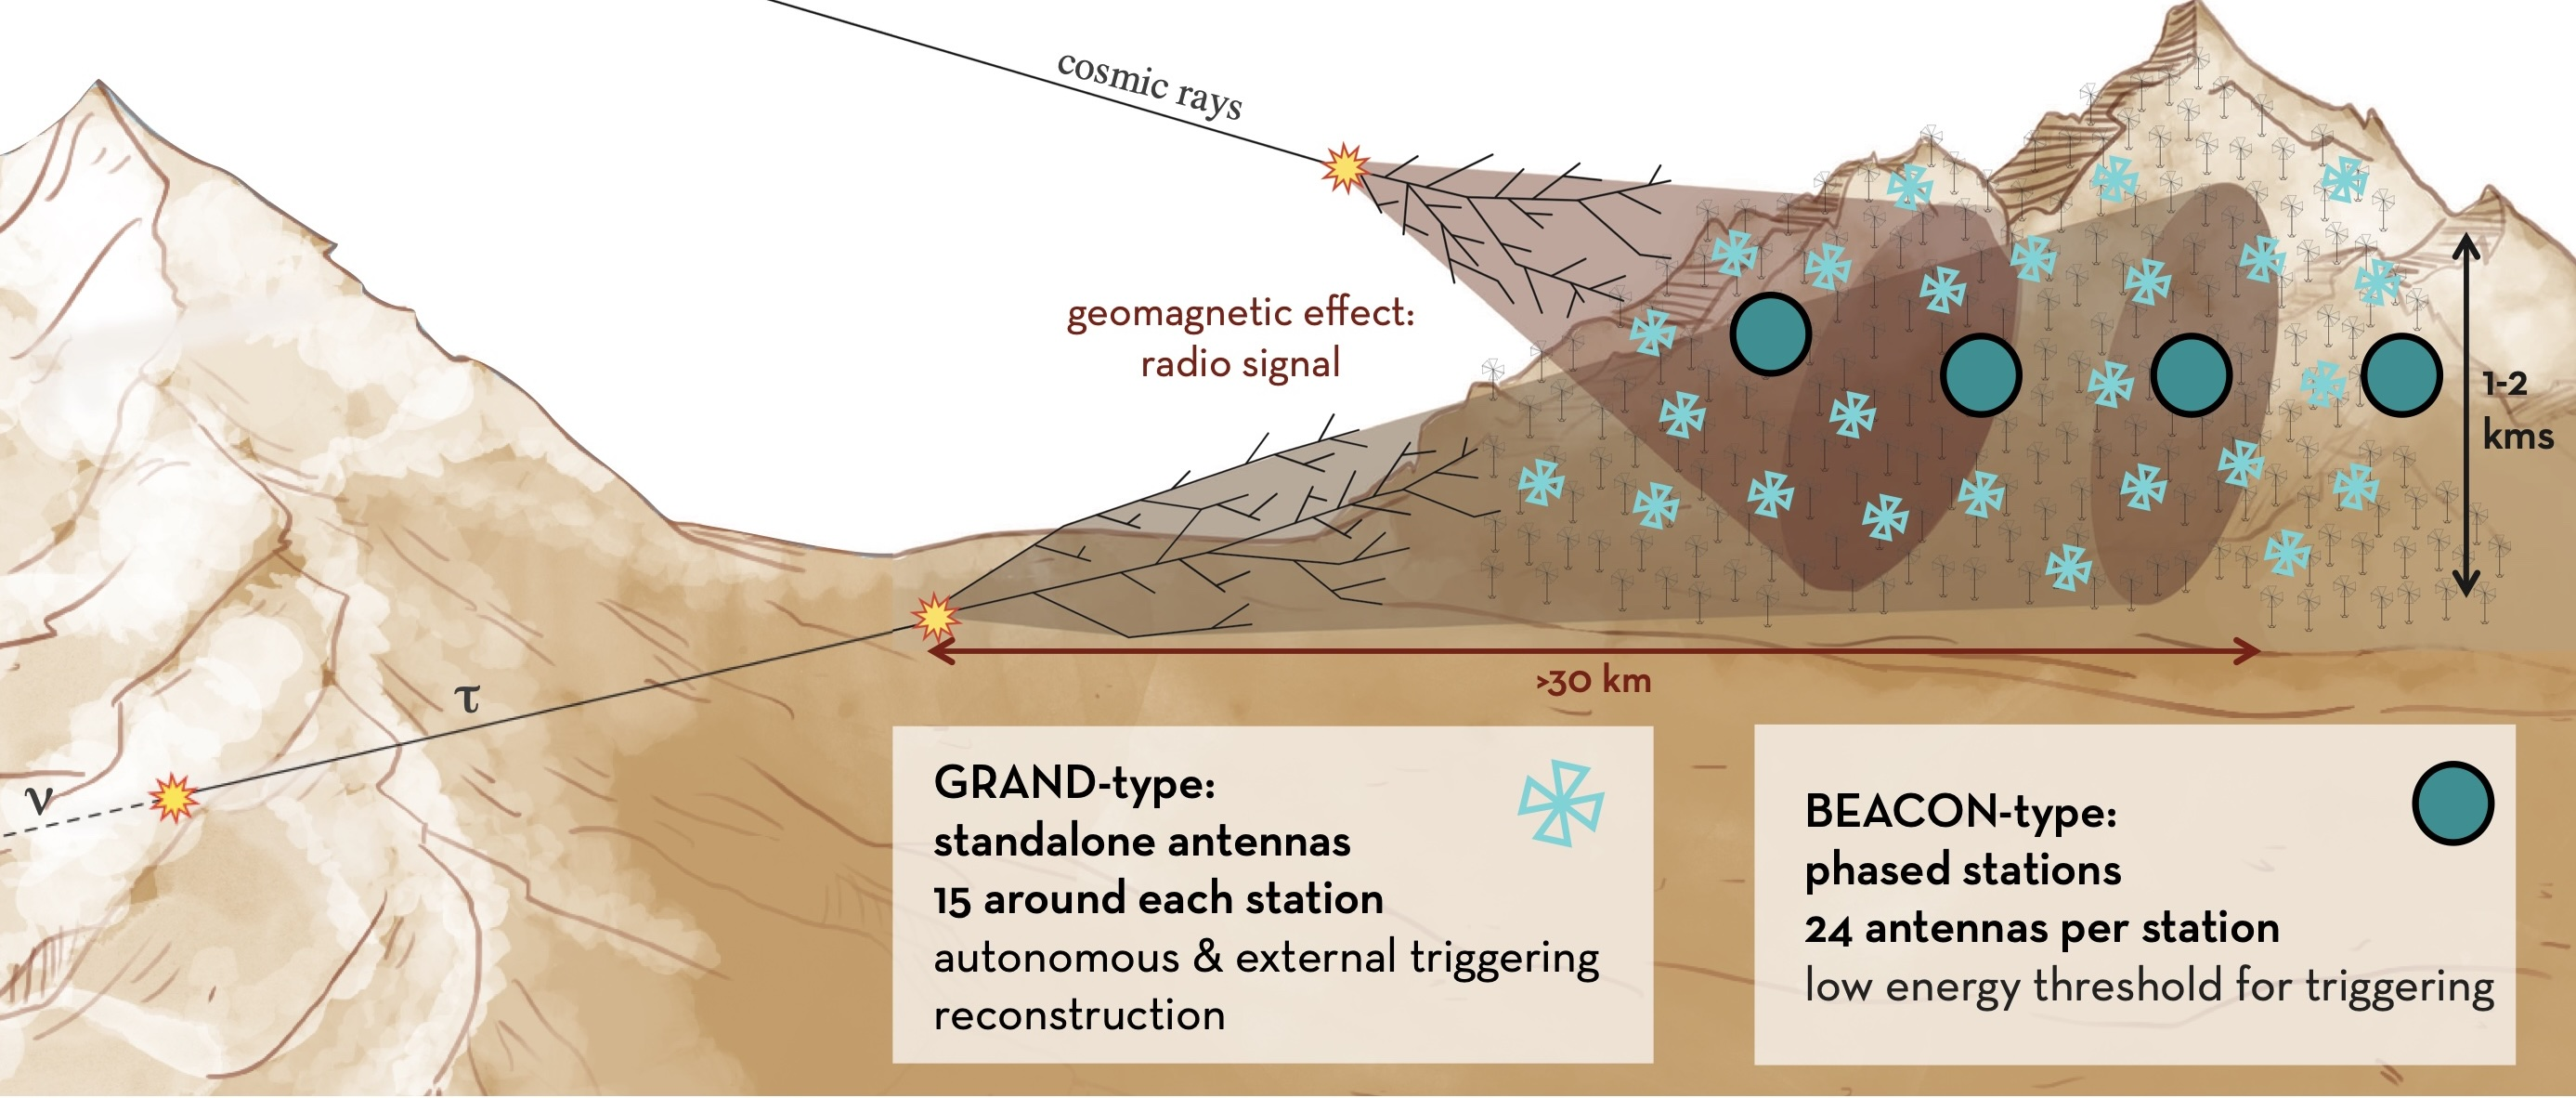
\includegraphics[width=0.66\linewidth]{heron/heron_concepto.png}\\[0pt]
  \begin{columns}[T,onlytextwidth]
    \column{0.50\textwidth}
      \footnotesize
      \begin{itemize}\footnotesize
        \item Un $\nu_\tau$ \textbf{roza la Tierra} y atraviesa la montaña:
          sale un $\tau$ que decae en el aire.
        \item Antenas en una ladera de \textbf{San Juan}, entre 1 y 2\,km sobre
          el valle.
      \end{itemize}
    \column{0.47\textwidth}
      \footnotesize
      \begin{itemize}\footnotesize
        \item \textbf{Híbrido}: 24 estaciones \emph{en fase} (BEACON) disparan;
          360 antenas autónomas (GRAND) reconstruyen.
        \item Objetivo: $\nu$ de $\sim$100\,PeV y \textbf{transitorios}.
      \end{itemize}
  \end{columns}
  \credito{Figura: K.~Kotera \textit{et al.} (BEACON y GRAND), PoS(ICRC2025), arXiv:2507.04382}
\end{frame}

% ---------------------------------------------------------------- 54
\begin{frame}{HERON desde San Juan}
  \begin{columns}[c,onlytextwidth]
    \column{0.36\textwidth}
      \centering
      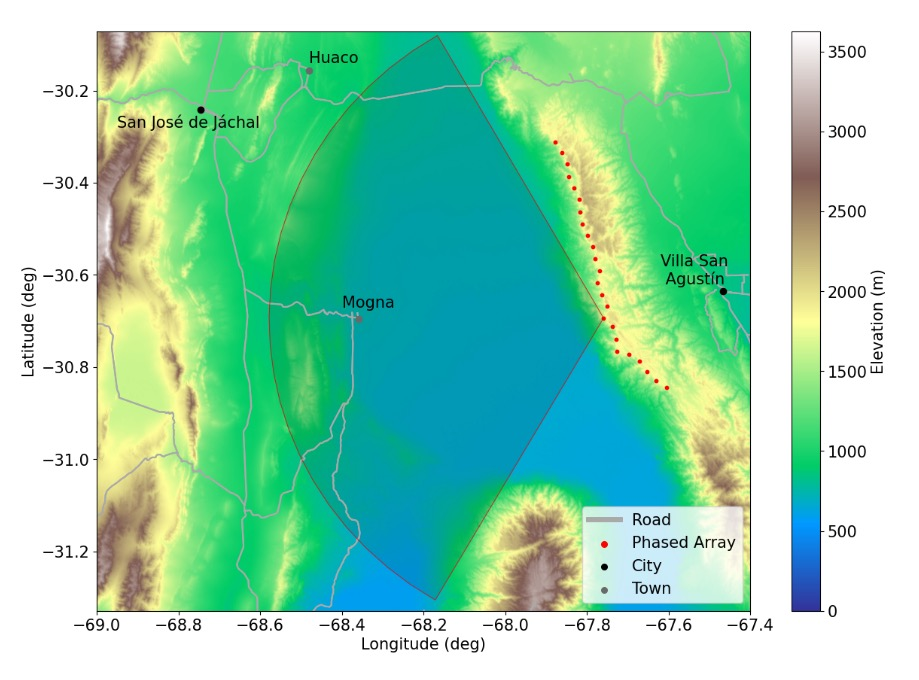
\includegraphics[width=0.84\linewidth]{heron/heron_sitio_mapa.png}\\[1pt]
      {\scriptsize 24 estaciones a lo largo de $\sim$70\,km de sierra, mirando
      un valle de 30--100\,km}
    \column{0.36\textwidth}
      \centering
      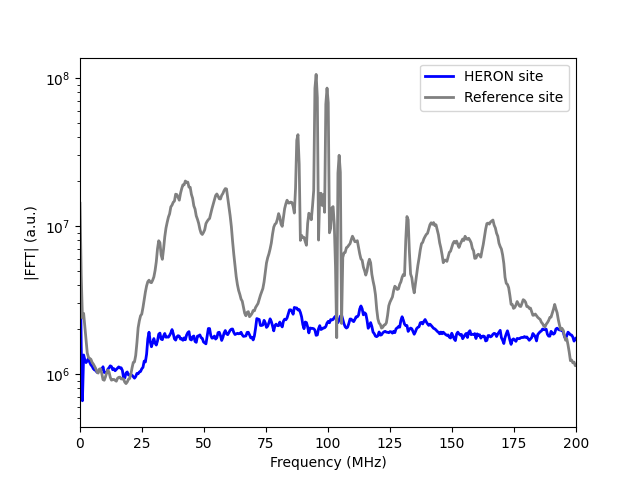
\includegraphics[width=0.88\linewidth]{heron/heron_ruido_sitio.png}\\[1pt]
      {\scriptsize Ruido de radio medido en el sitio (azul) frente a uno cerca
      de la ciudad (gris), abril de 2022}
    \column{0.25\textwidth}
      \begin{itemize}\scriptsize
        \item 936 antenas en total.
        \item Ve el 6\% del cielo a la vez y el 70\% por día.
        \item Proyecto de \textbf{I+D}, con diseño en optimización. Financiado
          por una \textbf{ERC Synergy Grant} y la ANR (Francia).
        \item CNEA (ITeDA, CAB), IAP--Sorbonne, IGFAE, Penn State.
      \end{itemize}
  \end{columns}
  \vspace{2pt}
  \begin{clave}
    No es un IceCube más grande: usa \textbf{la montaña como blanco} y
    \textbf{la atmósfera como calorímetro}.
  \end{clave}
  \creditoizq{Figuras: arXiv:2507.04382. Financiamiento y diseño: Zeolla, arXiv:2605.12081. Institucional: ITeDA}
\end{frame}

% ---------------------------------------------------------------- 55
\begin{frame}{HERON: cobertura del cielo y fuentes transitorias}
  \begin{columns}[c,onlytextwidth]
    \column{0.55\textwidth}
      \centering
      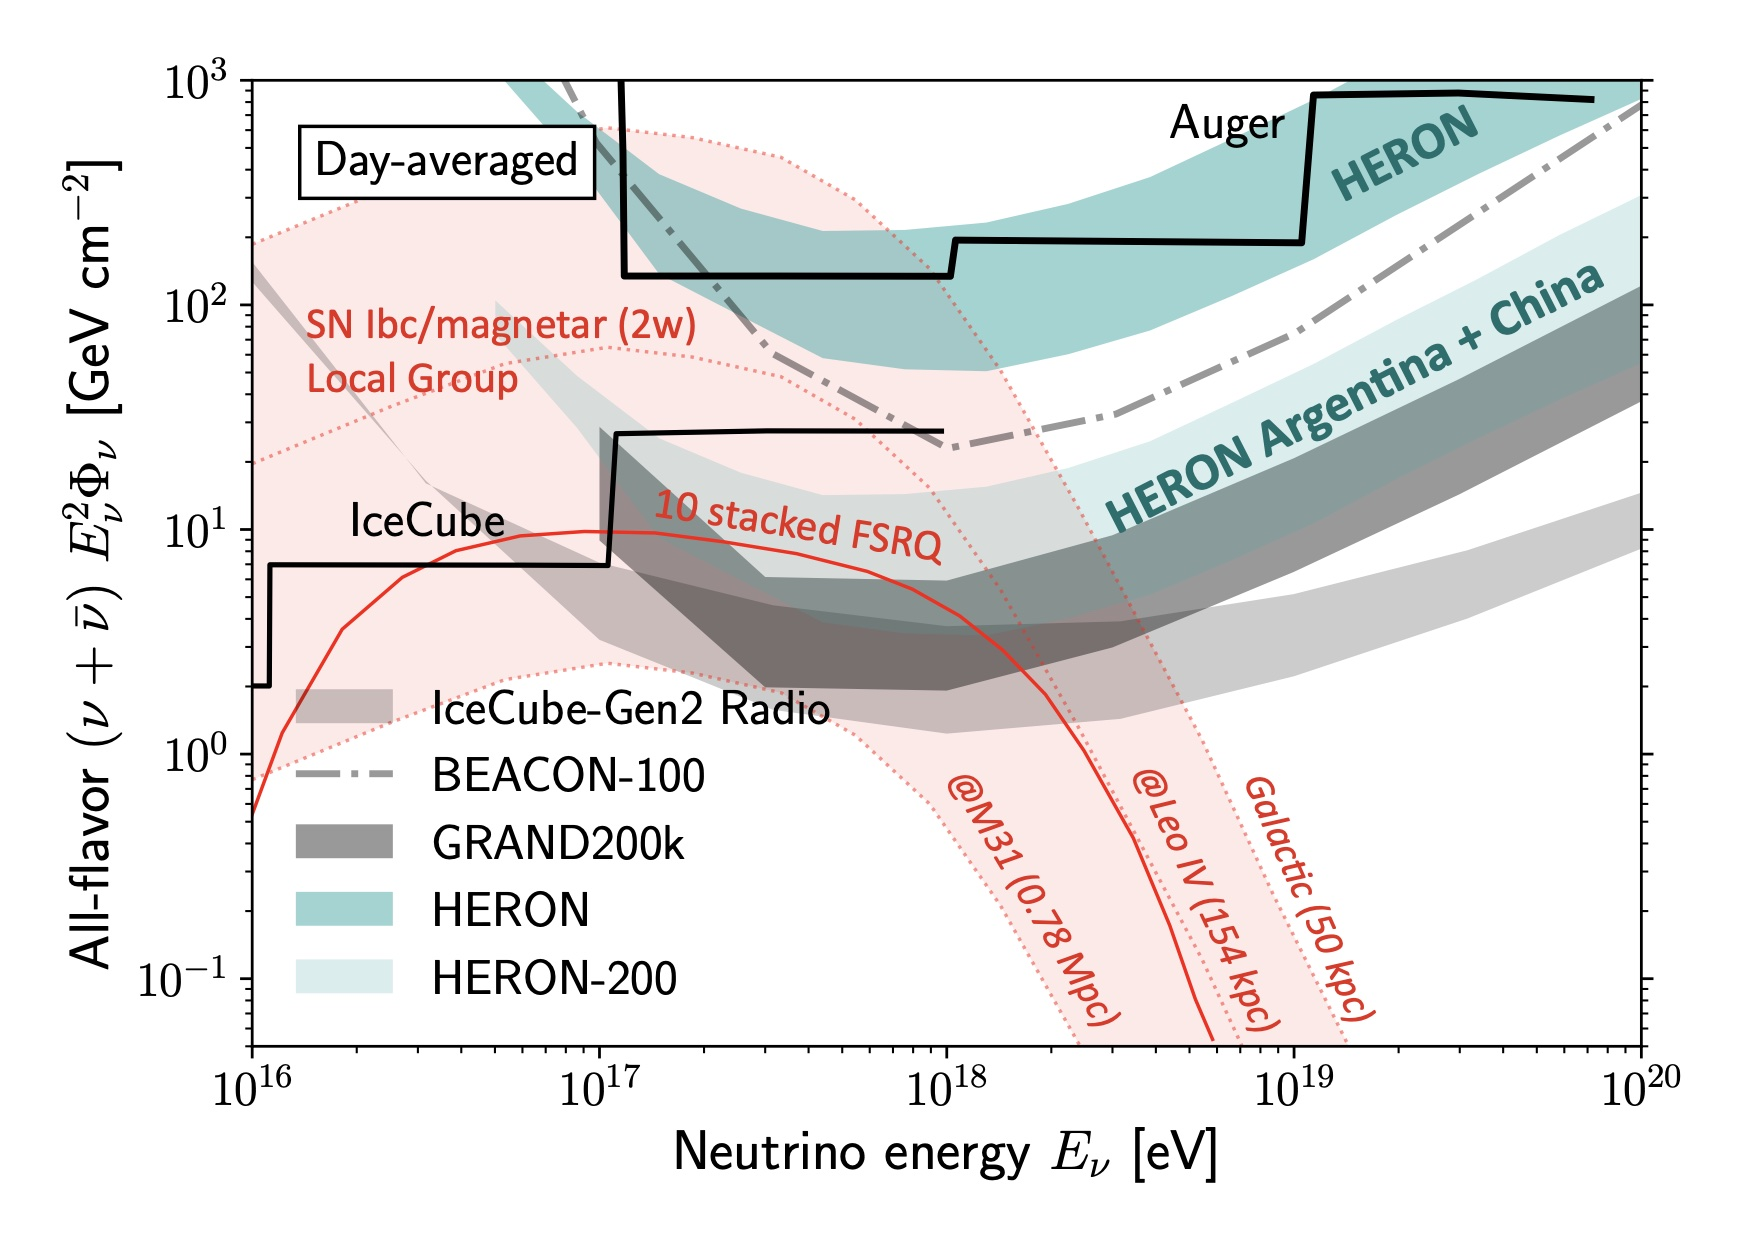
\includegraphics[width=\linewidth]{heron/heron_sensibilidad_dia.png}
    \column{0.42\textwidth}
      \small
      Sensibilidad promediada en un día, frente a IceCube, Auger y otros
      proyectos de radio (BEACON, GRAND, IceCube-Gen2 Radio).
      \begin{clave}
        HERON apunta a fuentes \textbf{transitorias} ---estallidos de rayos
        gamma, magnetares recién nacidos---, dentro de la red mundial de
        alertas multimensajero.
      \end{clave}
      {\footnotesize Para estallidos cortos, $\sim$10 veces mejor que los
      límites actuales de IceCube y Auger.}
  \end{columns}
  \credito{arXiv:2507.04382, Fig.~6; Zeolla, arXiv:2605.12081}
\end{frame}

% ---------------------------------------------------------------- 56
\begin{frame}{HERON frente a IceCube}
  \begin{columns}[c,onlytextwidth]
    \column{0.56\textwidth}
    \begin{tikzpicture}
      \begin{loglogaxis}[coloquio, width=\linewidth, height=6.1cm,
        xmin=1e15, xmax=1e20, ymin=1, ymax=2e7,
        xlabel={energía del neutrino [eV]}, ylabel={área efectiva [m$^2$]},
        xtick={1e15,1e16,1e17,1e18,1e19,1e20},
        ytick={1,1e2,1e4,1e6}, grid=major,
        legend style={at={(0.98,0.03)}, anchor=south east, font=\scriptsize,
          fill=white, fill opacity=0.9, text opacity=1, draw=itedaGray!40}]
        \fill[itedaOrange!14] (axis cs:5e16,1) rectangle (axis cs:2e17,2e7);
        \addplot[very thick, cmbAzul] table[x=E_eV, y expr=\thisrow{A_km2}*1e6] {data/icecube_aeff.dat};
        \addlegendentry{IceCube (todo el cielo)}
        \addplot[very thick, verdeRadio, dashed] table[x=E_eV, y expr=\thisrow{A_km2}*1e6] {data/heron_aeff_aprox.dat};
        \addlegendentry{HERON (en su franja del cielo)}
        \node[font=\scriptsize\bfseries, text=itedaOrange, anchor=north] at (axis cs:1e17,1.6e7) {$10^{17}$\,eV};
        \node[font=\scriptsize\bfseries, text=cmbAzul, fill=white, inner sep=1pt, anchor=north west]
          at (axis cs:1.3e17,700) {$\sim$1.000\,m$^2$};
        \node[font=\scriptsize\bfseries, text=verdeRadio, fill=white, inner sep=1pt, anchor=south east]
          at (axis cs:9e16,3e4) {$\sim$30.000\,m$^2$};
        \draw[-{Stealth}, itedaGray] (axis cs:2e15,300) -- (axis cs:5.5e15,170);
        \node[font=\tiny, text=itedaGray, anchor=south] at (axis cs:2e15,300) {Glashow};
      \end{loglogaxis}
    \end{tikzpicture}
    \column{0.41\textwidth}
      \tikzset{cab/.style={font=\scriptsize\bfseries, text=white, rounded corners=1.5pt,
        minimum width=2.3cm, minimum height=0.45cm}}
      \renewcommand{\arraystretch}{1.2}
      \vspace*{-6pt}
      {\tiny
      \begin{tabular}{@{}>{\raggedright\arraybackslash}p{0.95cm}>{\raggedright\arraybackslash}p{2.3cm}>{\raggedright\arraybackslash}p{2.3cm}@{}}
        & \tikz\node[cab, fill=cmbAzul]{IceCube}; & \tikz\node[cab, fill=verdeRadio]{HERON};\\
        \textbf{Tamaño} & 1\,km$^3$ de hielo, 5160 sensores & $\sim$70\,km de sierra, 936 antenas\\
        \textbf{Energías} & $10^{10}$--$10^{16}$\,eV & $>10^{16}$\,eV, óptimo $10^{17}$\,eV\\
        \textbf{Cielo} & todo, siempre & 6\% a la vez, 70\% por día\\
        \textbf{Área a $10^{17}$\,eV} & $\sim$1.000\,m$^2$ & $\sim$30.000\,m$^2$\\
        \textbf{Eventos} & $\sim$100 sobre 60\,TeV en 7,5 años; ninguno firme sobre 10\,PeV & meta: $\nu$ de $\sim$200 GRB en 5--10 años\\
      \end{tabular}}\\[4pt]
      \begin{clave}[fontupper=\footnotesize]
        IceCube domina hasta el PeV. A $10^{17}$--$10^{18}$\,eV, HERON ve
        10--100 veces más, pero sólo en una franja del cielo.
      \end{clave}
  \end{columns}
  \creditoizq{IceCube: data release EHE (arXiv:2507.07497), HESE 7,5 años. HERON: arXiv:2507.04382, Fig.~4, leída a ojo}
\end{frame}

% ---------------------------------------------------------------- 57
\begin{frame}{Una red mundial de telescopios de neutrinos}
  \begin{columns}[c,onlytextwidth]
    \column{0.55\textwidth}
      \centering
      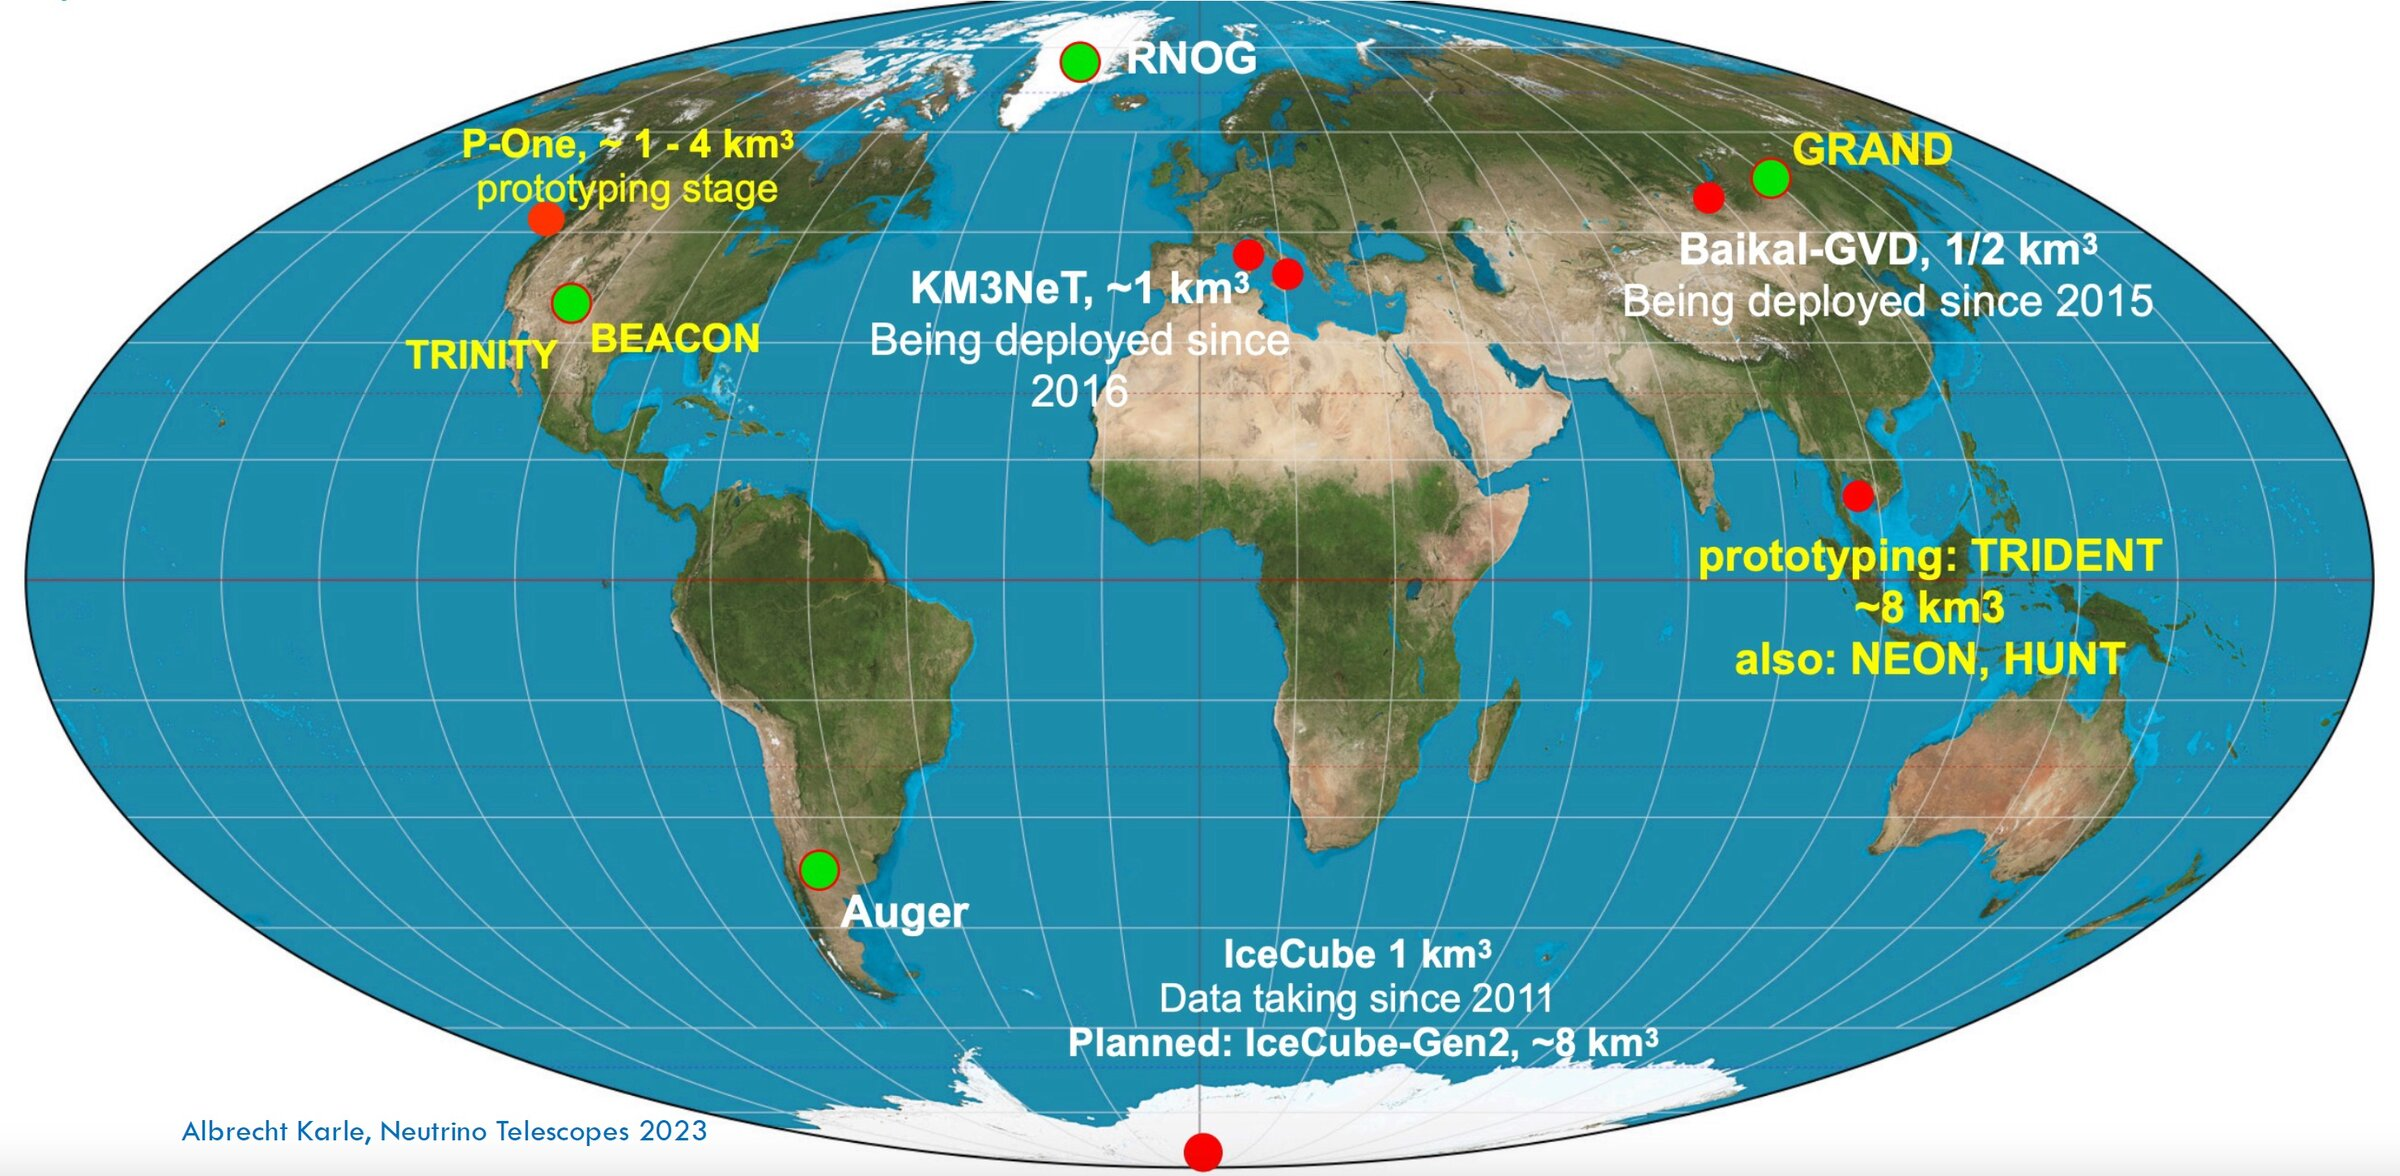
\includegraphics[width=\linewidth]{halzen/telescopios_neutrinos_mapa.jpg}
    \column{0.42\textwidth}
      \centering
      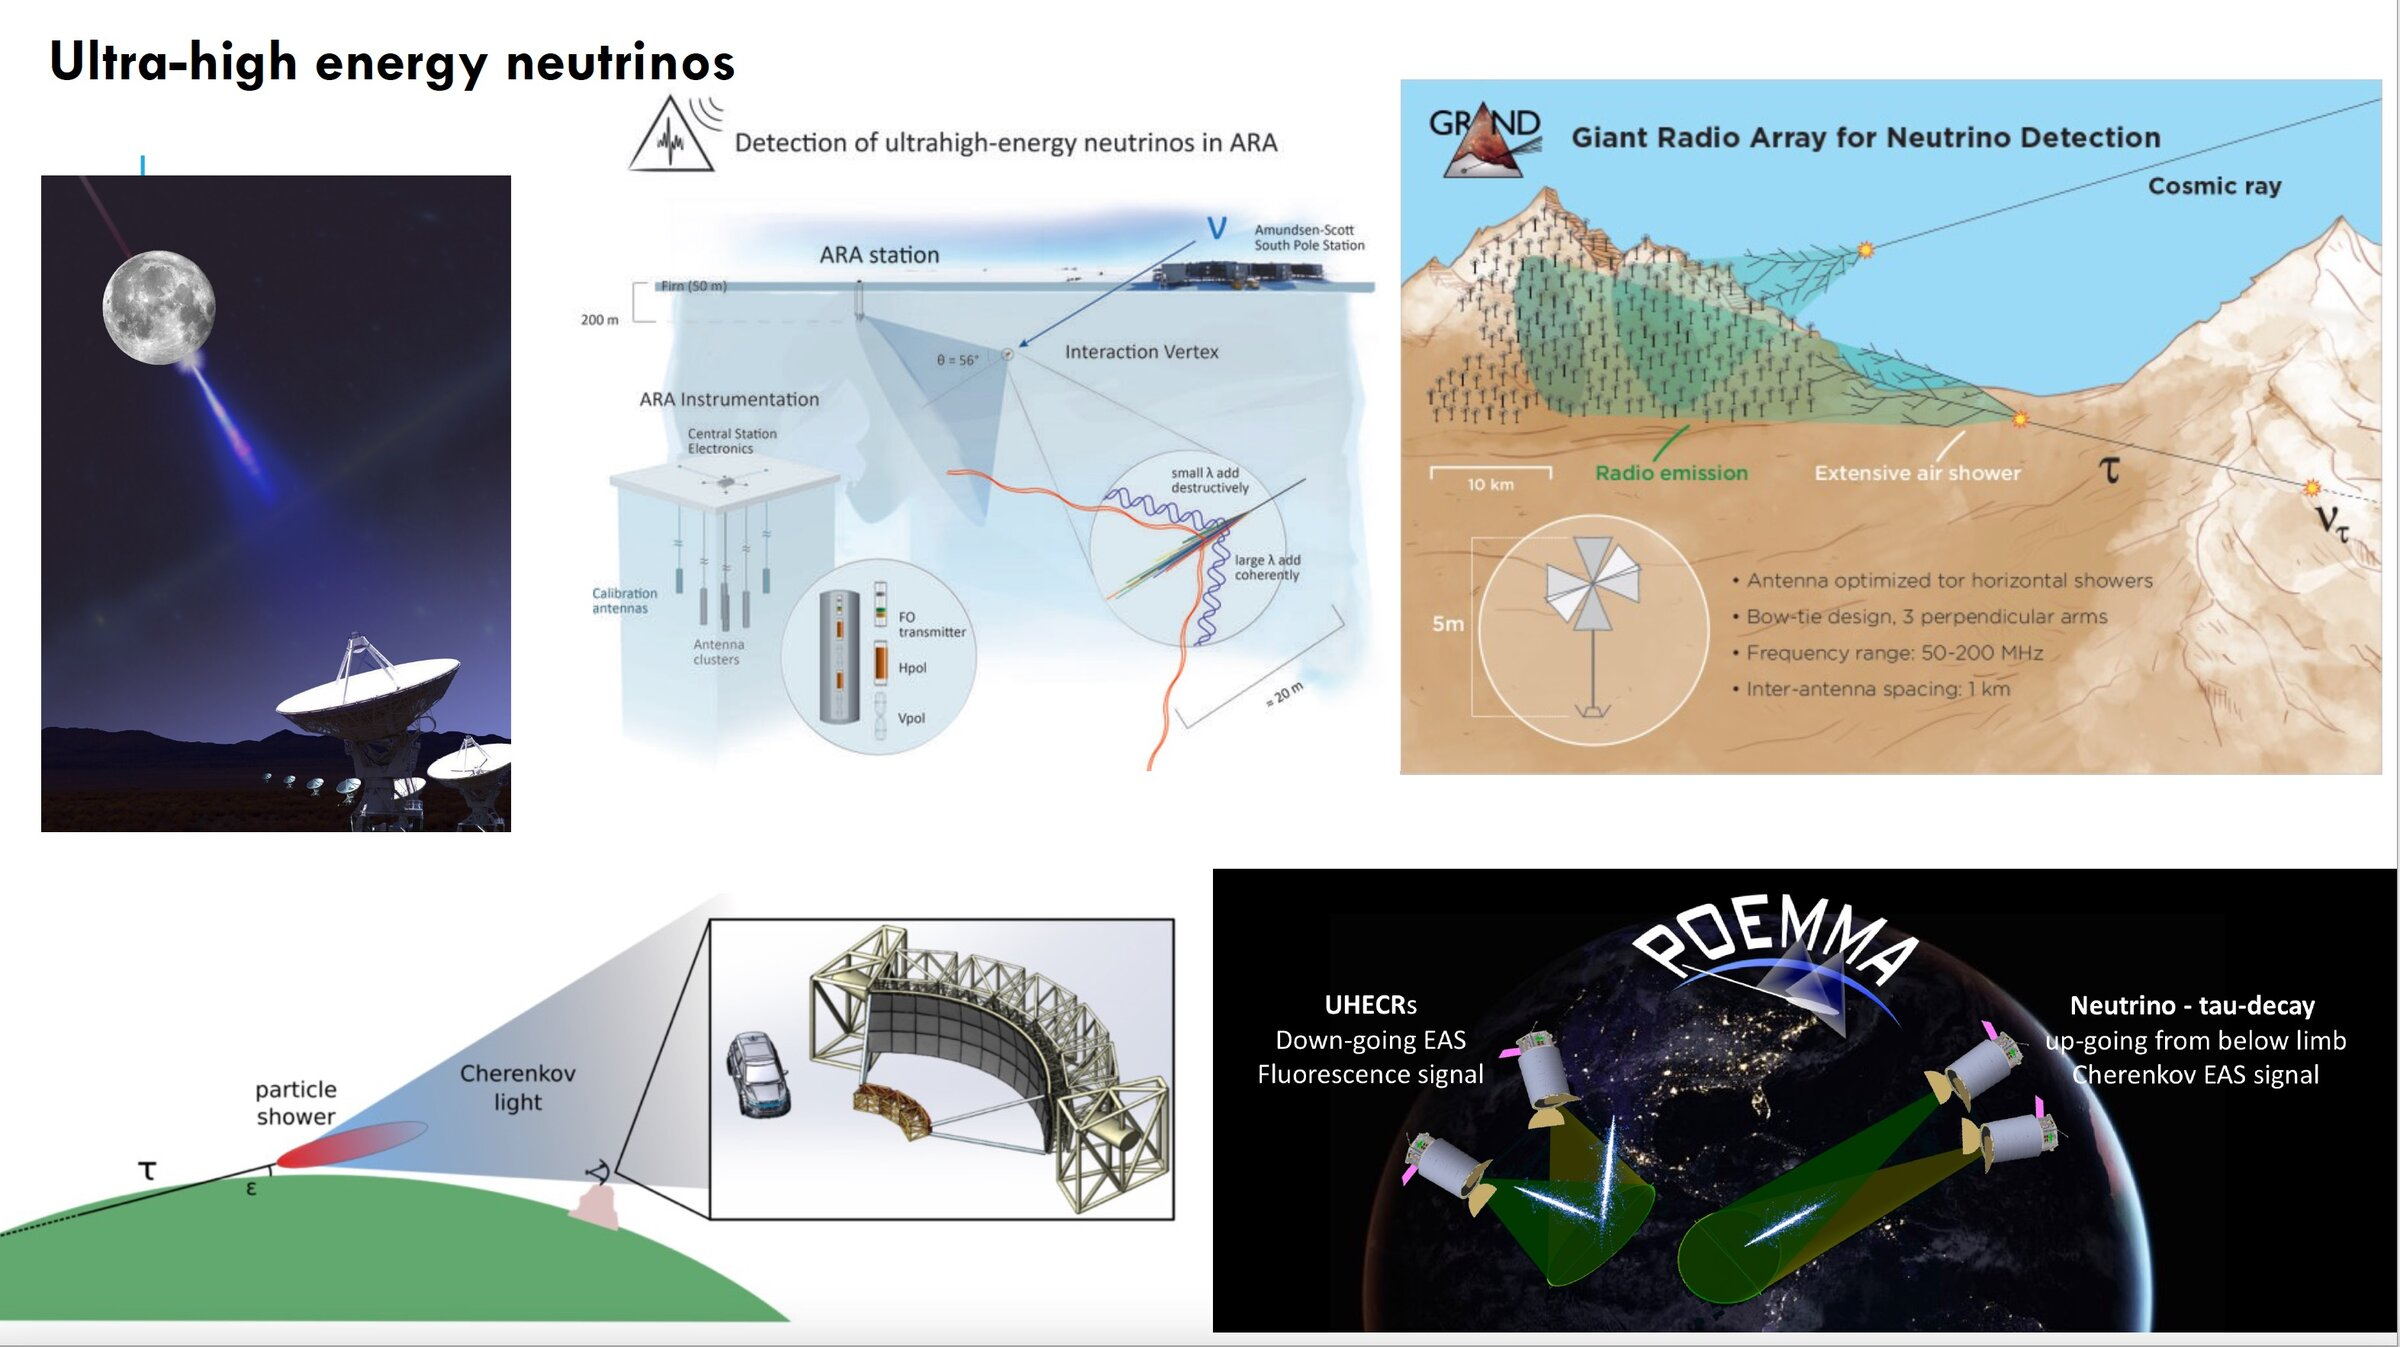
\includegraphics[width=\linewidth]{halzen/uhe_neutrinos_conceptos.jpg}\\[2pt]
      {\footnotesize Técnicas para ultra alta energía: radio en hielo, radio
      en el aire, lluvias de $\tau$ y observación desde el espacio. HERON
      suma a la Argentina a esa red.}
  \end{columns}
  \credito{Vía F.~Halzen (2024); mapa: A.~Karle, \textit{Neutrino Telescopes} 2022}
\end{frame}

% ---------------------------------------------------------------- 58
\bloque{CIERRE}
\begin{frame}{Tres soluciones experimentales a tres problemas físicos}
  \begin{tikzpicture}[x=1cm,y=1cm]
    \tikzset{
      cab/.style={font=\small\bfseries, text=white, minimum width=3.65cm,
        minimum height=0.6cm, rounded corners=2pt},
      celda/.style={font=\scriptsize, text width=3.5cm, align=left, anchor=north west},
      lab/.style={font=\scriptsize\bfseries, text=itedaGray, anchor=north east, align=right}}
    \node[cab, fill=itedaOrange] at (4.25,0) {Pierre Auger};
    \node[cab, fill=cmbAzul] at (8.1,0) {IceCube};
    \node[cab, fill=verdeRadio] at (11.95,0) {HERON};
    \foreach \y/\l/\a/\b/\c in {
        -0.5/{Mensajero}/{Rayos cósmicos}/{Neutrinos}/{$\nu_\tau$ que rozan la Tierra},
        -1.2/{Señal}/{Suelo, fluorescencia, radio}/{Luz Cherenkov en el hielo}/{Radio de lluvias en el aire},
        -1.9/{Geometría}/{Superficie de 3000\,km$^2$}/{Volumen de 1\,km$^3$}/{Ladera que mira un valle},
        -2.6/{Objetivo}/{Origen y composición de las partículas más energéticas}/{Dónde se aceleran los hadrones}/{$\nu$ de $\sim$100\,PeV y transitorios}}{
      \node[lab] at (2.3,\y) {\l};
      \node[celda] at (2.45,\y) {\a};
      \node[celda] at (6.3,\y) {\b};
      \node[celda] at (10.15,\y) {\c};
      \draw[itedaGray!30] (0.6,\y+0.08) -- (13.9,\y+0.08);}
    % eje de energía
    \begin{scope}[yshift=-4.75cm]
      \draw[itedaGray, thick, -{Stealth}] (2.3,0) -- (13.9,0);
      \foreach \e in {10,12,...,20}{
        \pgfmathsetmacro{\xx}{2.3+(\e-10)*1.05}
        \draw[itedaGray] (\xx,-0.07) -- (\xx,0.07) node[below=2pt, font=\tiny] {$10^{\e}$};}
      \node[lab, anchor=east] at (2.3,0.25) {Energía [eV]};
      \fill[cmbAzul, rounded corners=1pt] ({2.3+0*1.05},0.12) rectangle ({2.3+6*1.05},0.27);
      \node[font=\tiny\bfseries, text=cmbAzul, anchor=south] at ({2.3+3*1.05},0.27) {IceCube};
      \fill[itedaOrange, rounded corners=1pt] ({2.3+7*1.05},0.12) rectangle ({2.3+10.4*1.05},0.27);
      \node[font=\tiny\bfseries, text=itedaOrange, anchor=west] at ({2.3+10.45*1.05},0.2) {Auger};
      \fill[verdeRadio, rounded corners=1pt] ({2.3+6.7*1.05},0.36) rectangle ({2.3+9*1.05},0.51);
      \node[font=\tiny\bfseries, text=verdeRadio, anchor=east] at ({2.3+6.65*1.05},0.44) {HERON};
    \end{scope}
  \end{tikzpicture}
  \creditoizq{Rangos de energía aproximados}
\end{frame}

% ---------------------------------------------------------------- 59
\bloque{}
\begin{frame}[plain]
  \fondo[0.0][h]{tesis/auger_cr.jpg}
  \velo[0.75]{l}
  \begin{tikzpicture}[remember picture, overlay]
    \node[anchor=north west, text=white, align=left]
      at ([xshift=0.9cm, yshift=-0.9cm]current page.north west) {%
      {\fontsize{34}{38}\selectfont\bfseries ¡Gracias!}\\[6pt]
      {\Large\color{itedaOrange}\bfseries ¿Preguntas?}};
    \node[anchor=south west, text=white, align=left]
      at ([xshift=0.9cm, yshift=0.9cm]current page.south west) {%
      {\small Lautaro Silva Pizzi · ITeDA (CNEA--CONICET--UNSAM)}\\[2pt]
      {\small lautarosilvapizzi@gmail.com}};
    \node[anchor=south east, fill=white, rounded corners=2pt, inner sep=3pt]
      at ([xshift=-0.6cm, yshift=0.9cm]current page.south east)
      {
\includegraphics[height=0.95cm]{logos/logo-portada5-iteda.png}};
  \end{tikzpicture}
  \creditoblanco{Imagen: A.~Chantelauze, S.~Staffi, L.~Bret (Observatorio Pierre Auger)}
\end{frame}


\appendix
% ======================================================================
% DIAPOSITIVAS DE RESPALDO (no se numeran con la charla principal)
% ======================================================================
\section{Respaldo}
\bloque{RESPALDO}

% ---------------------------------------------------------------- R0
\begin{frame}[plain]
  \begin{tikzpicture}[remember picture, overlay]
    \fill[itedaTeal] (current page.south west) rectangle (current page.north east);
    \node[text=white, font=\fontsize{26}{30}\selectfont\bfseries] at (current page.center)
      {Respaldo};
    \node[text=white!80, font=\small, anchor=north] at ([yshift=-0.7cm]current page.center)
      {cálculos, figuras adicionales de la tesis y material de referencia};
  \end{tikzpicture}
\end{frame}

% ---------------------------------------------------------------- R1
\begin{frame}{Respaldo: las cuentas de las escalas de energía y flujo}
  \begin{columns}[T,onlytextwidth]
    \column{0.49\textwidth}
      \small
      \textbf{Energía}
      \[ 1\,\mathrm{eV}=1{,}602\times10^{-19}\,\mathrm{J}
         \;\Rightarrow\; 10^{20}\,\mathrm{eV}=16{,}0\,\mathrm{J} \]
      \[ \tfrac12(0{,}145\,\mathrm{kg})(25\,\mathrm{m/s})^2=45{,}3\,\mathrm{J}
         \approx 2{,}8\times10^{20}\,\mathrm{eV} \]
      \textbf{Centro de masa} (blanco en reposo, $E\gg m$)
      \[ \sqrt{s}=\sqrt{2Em_pc^2}:\quad
         \begin{cases}10^{17}\,\mathrm{eV}\to 13{,}7\,\mathrm{TeV}\\
         10^{20}\,\mathrm{eV}\to 433\,\mathrm{TeV}\end{cases} \]
    \column{0.48\textwidth}
      \small
      \textbf{Tasa en Auger}
      \[ \frac{\approx5\times10^4\ \text{eventos}}{19\ \text{años}\times3000\,\mathrm{km^2}}
         \approx 0{,}9\ \mathrm{km^{-2}\,año^{-1}}\quad(E>8\,\mathrm{EeV}) \]
      Exposición acumulada: $\approx1{,}2\times10^{5}$\,km$^2$\,sr\,año (ICRC 2025).\\[6pt]
      \textbf{Cherenkov}
      \[ \frac{d^2N}{dx\,d\lambda}=\frac{2\pi\alpha}{\lambda^2}
         \Big(1-\frac{1}{\beta^2n^2}\Big) \]
      {\footnotesize En agua, entre 300 y 600\,nm: $\approx330$ fotones/cm para
      $\beta\to1$. Umbral $\gamma=1{,}52$: $T_e=0{,}26$\,MeV, $T_\mu=55$\,MeV.}
  \end{columns}
\end{frame}

% ---------------------------------------------------------------- R2
\begin{frame}{Respaldo: el modelo analítico de la asimetría (tesis, Cap.~3)}
  \begin{columns}[c,onlytextwidth]
    \column{0.62\textwidth}
      \centering
      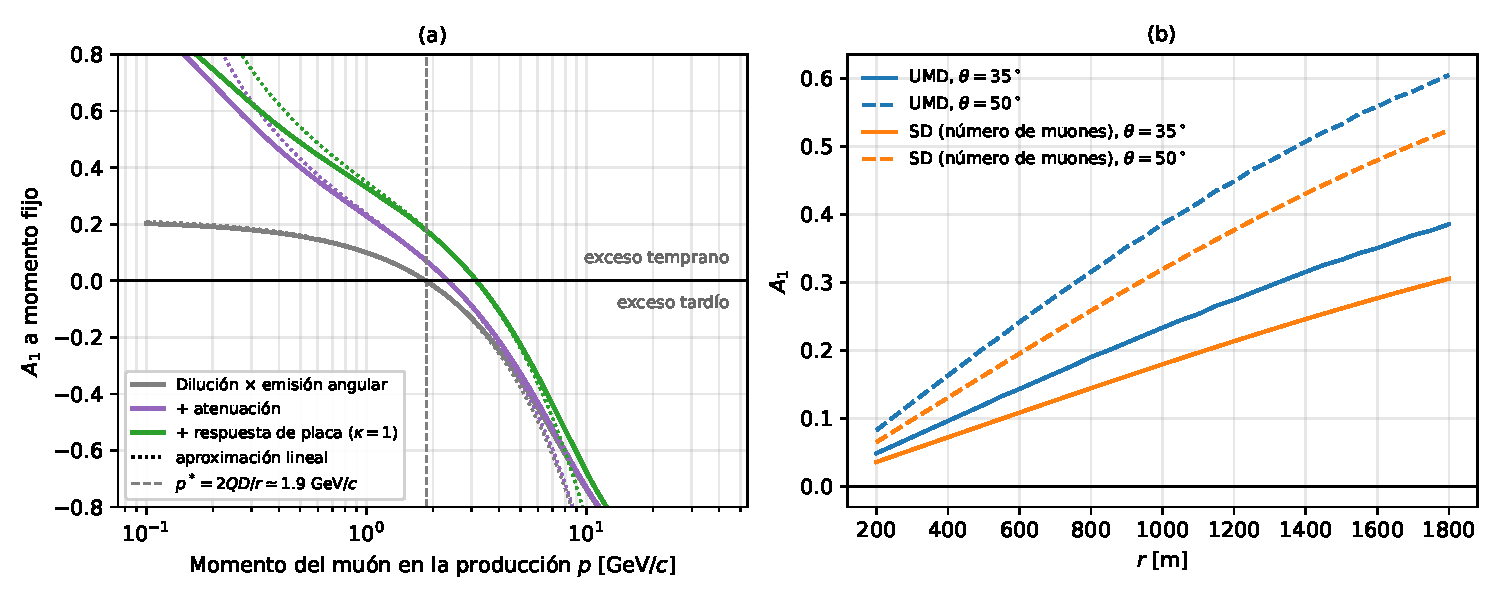
\includegraphics[width=\linewidth]{tesis/modelo_juguete.pdf}
    \column{0.35\textwidth}
      \small
      Reúne dilución, atenuación, respuesta del detector y divergencia
      cinemática. Predice $A_1>0$ en el UMD y el SD, creciente con $r$ y $\theta$.
      \begin{clave}
        La divergencia favorece la región tardía sólo para
        $p > p^*\simeq 2QD/r$: esos muones escasean lejos del núcleo.
      \end{clave}
  \end{columns}
\end{frame}

% ---------------------------------------------------------------- R3
\begin{frame}{Respaldo: sesgo direccional en la reconstrucción de $N_\mu$}
  \begin{columns}[c,onlytextwidth]
    \column{0.55\textwidth}
      \centering
      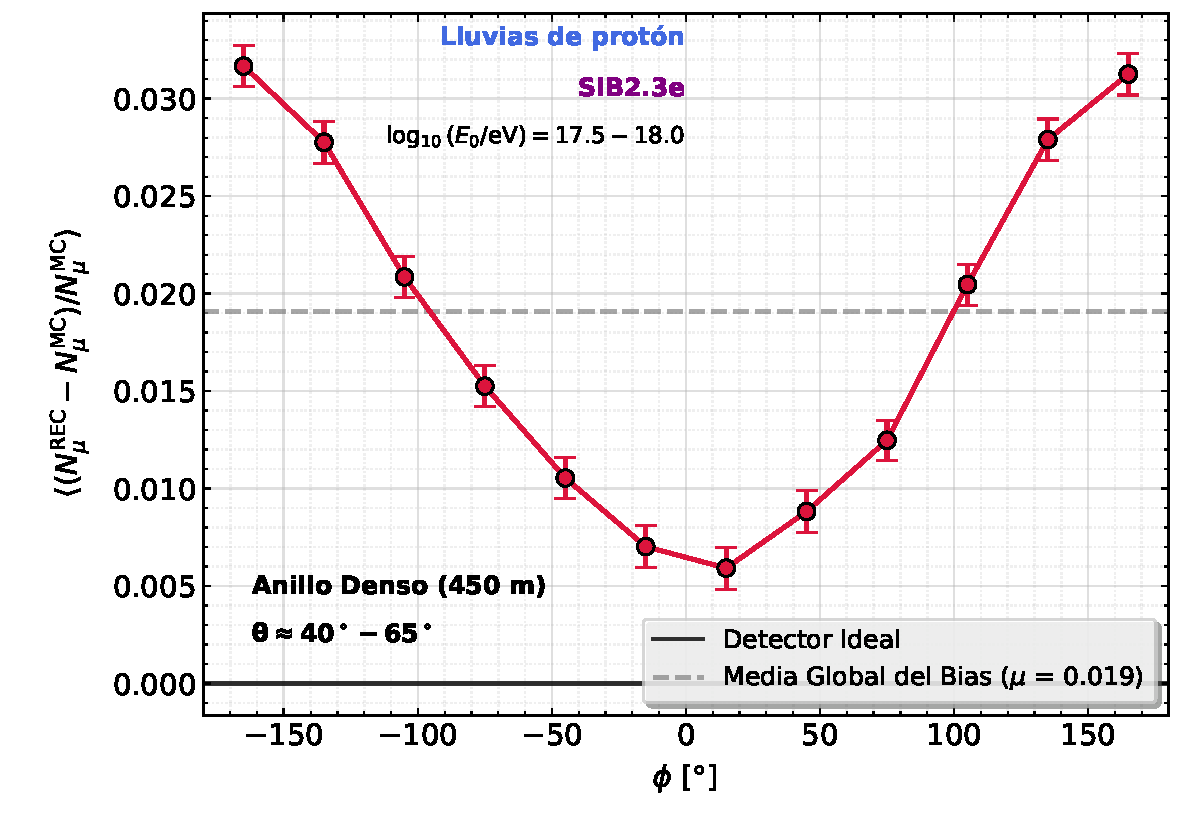
\includegraphics[width=\linewidth]{tesis/directional_bias.pdf}
    \column{0.42\textwidth}
      \small
      El sobreconteo medio es mayor del lado \textbf{tardío}, donde la
      densidad es menor: el error de reconstrucción depende del azimut.
      \begin{clave}
        Un modelo que inyecta los residuos empíricos por azimut reproduce la
        amplitud reconstruida hasta $\theta\approx35^\circ$ y explica la mitad
        o dos tercios de la pérdida más arriba.
      \end{clave}
  \end{columns}
  \credito{Anillo Denso, protones, SIBYLL 2.3e. Tesis, Cap.~5}
\end{frame}

% ---------------------------------------------------------------- R4
\begin{frame}{Respaldo: ¿quiénes quedan afuera de la selección?}
  \centering
  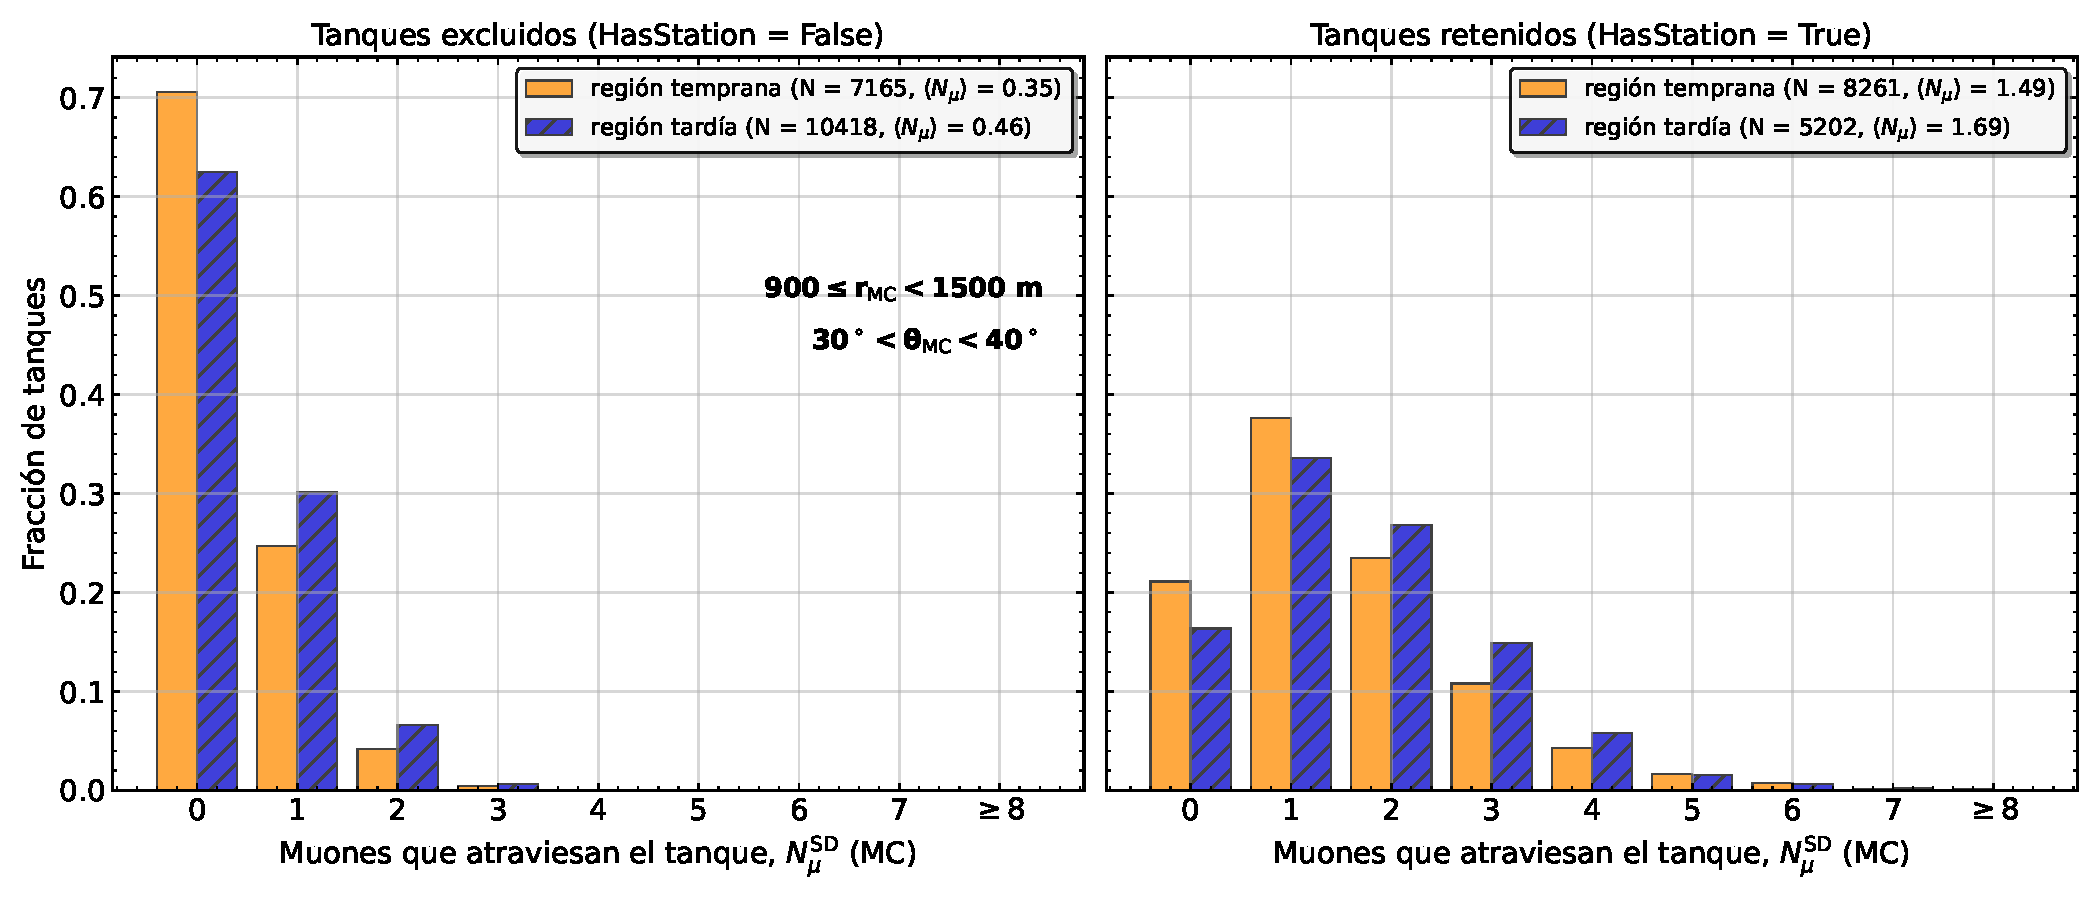
\includegraphics[width=0.8\linewidth]{tesis/SD_Muones_Tanques_Excluidos.pdf}\\[4pt]
  \begin{columns}[T,onlytextwidth]
    \column{0.48\textwidth}
      \footnotesize Tanques excluidos con $\le1$ muón: 95\% (tempranos) y
      93\% (tardíos); media 0,35 y 0,46.
    \column{0.48\textwidth}
      \footnotesize Retenidos: 1,49 (tempranos) y 1,69 (tardíos) muones, aunque
      la densidad incidente es mayor del lado temprano.
  \end{columns}
  \credito{$900\le r<1500$\,m, $30^\circ$--$40^\circ$, geometría MC. Tesis, Cap.~6}
\end{frame}

% ---------------------------------------------------------------- R5
\begin{frame}{Respaldo: el desglose de la señal del SD}
  \begin{columns}[c,onlytextwidth]
    \column{0.58\textwidth}
      \centering
      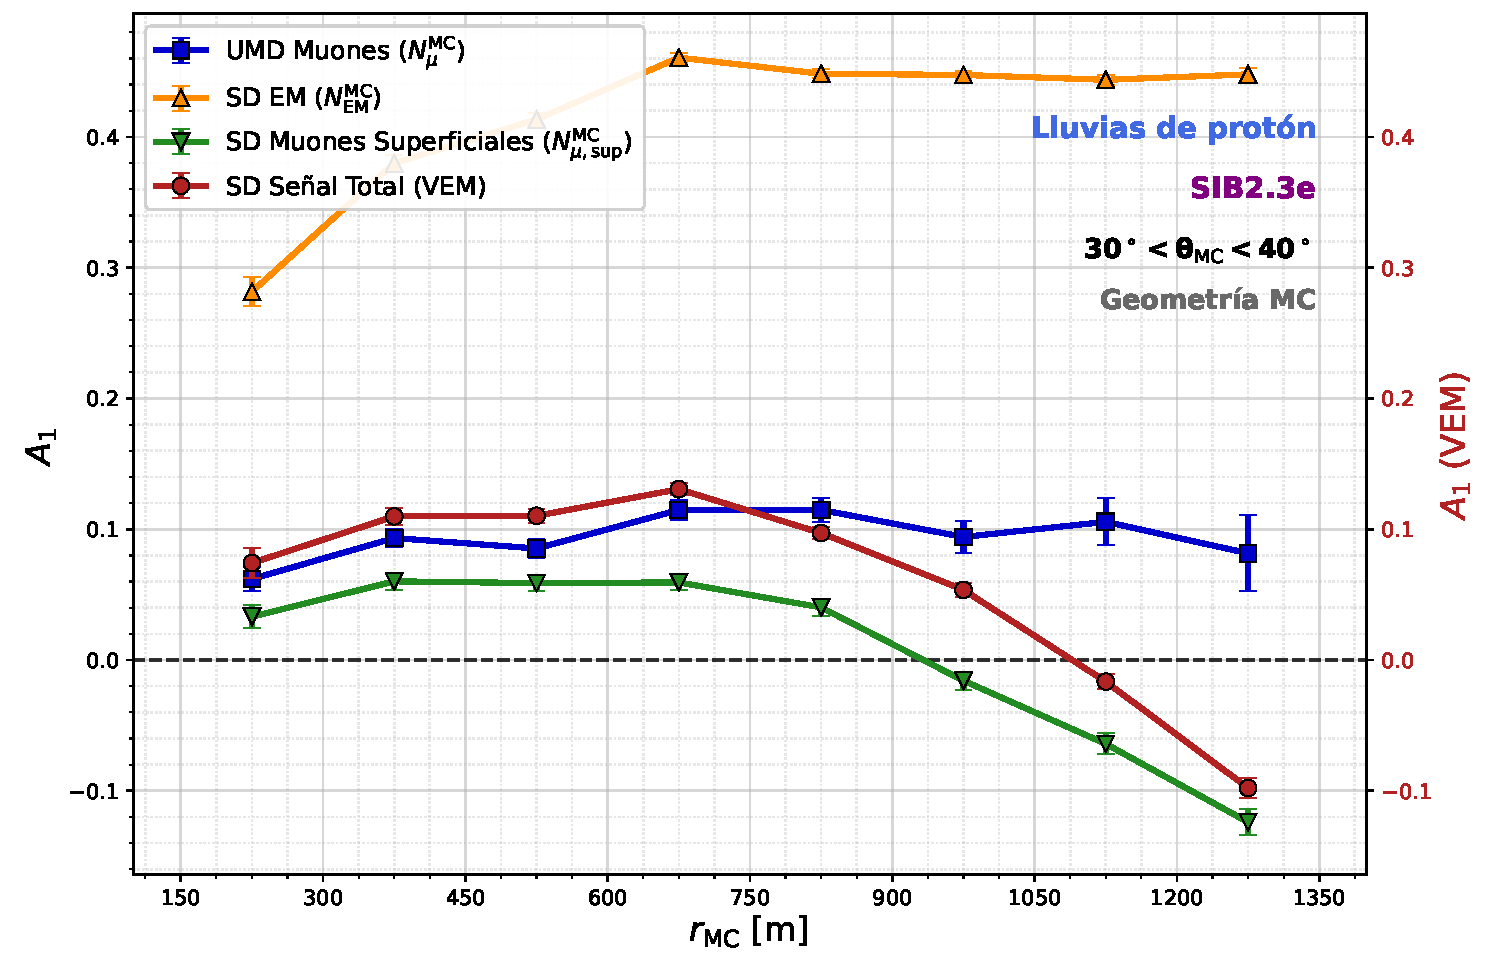
\includegraphics[width=\linewidth]{tesis/SD_Desglose_Componentes_vs_UMD.pdf}
    \column{0.39\textwidth}
      \small
      La componente electromagnética del SD es fuertemente positiva; los
      muones del SD, calculados sobre estaciones seleccionadas, se invierten
      lejos del núcleo y arrastran a la señal total.
      \begin{clave}
        Aun sin selección, entre 150 y 900\,m el UMD supera a los muones del SD
        en 0,03--0,06 (excluye cero al 95\%): diferencia abierta.
      \end{clave}
  \end{columns}
  \credito{Protones, $30^\circ$--$40^\circ$, geometría MC. Tesis, Cap.~6}
\end{frame}

% ---------------------------------------------------------------- R6
\begin{frame}{Respaldo: $A_1(r,\theta)$ en el arreglo de 750\,m}
  \begin{columns}[T,onlytextwidth]
    \column{0.49\textwidth}
      \centering
      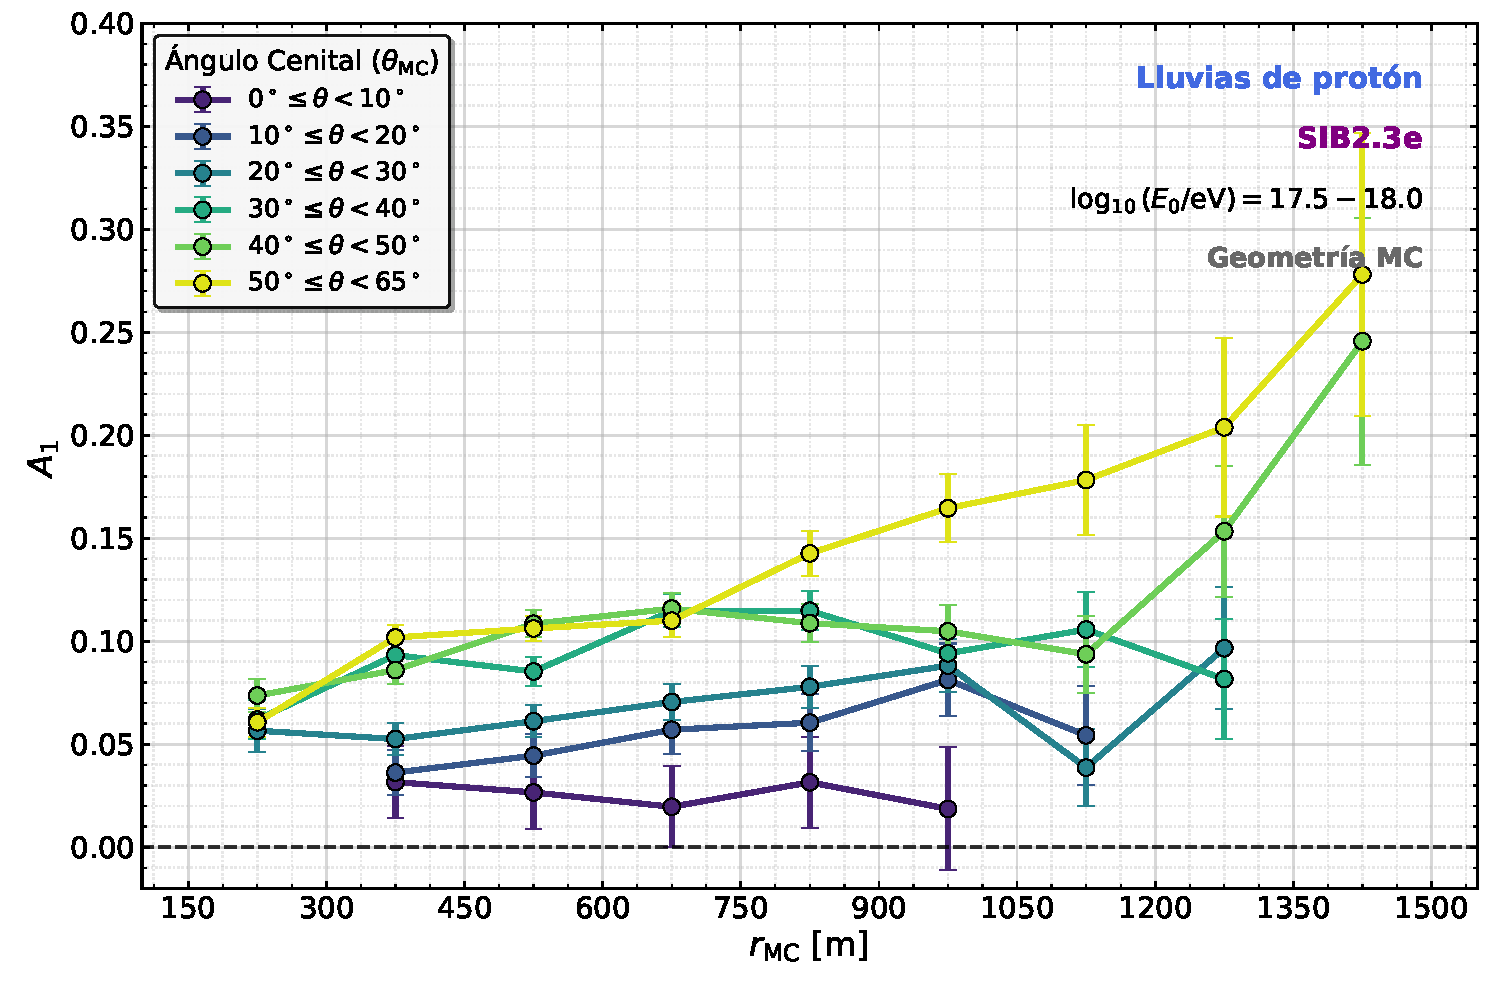
\includegraphics[width=\linewidth]{tesis/Global_A1_vs_R_Theta_MC.pdf}\\
      {\footnotesize Geometría MC: crece con $r$ y $\theta$.}
    \column{0.49\textwidth}
      \centering
      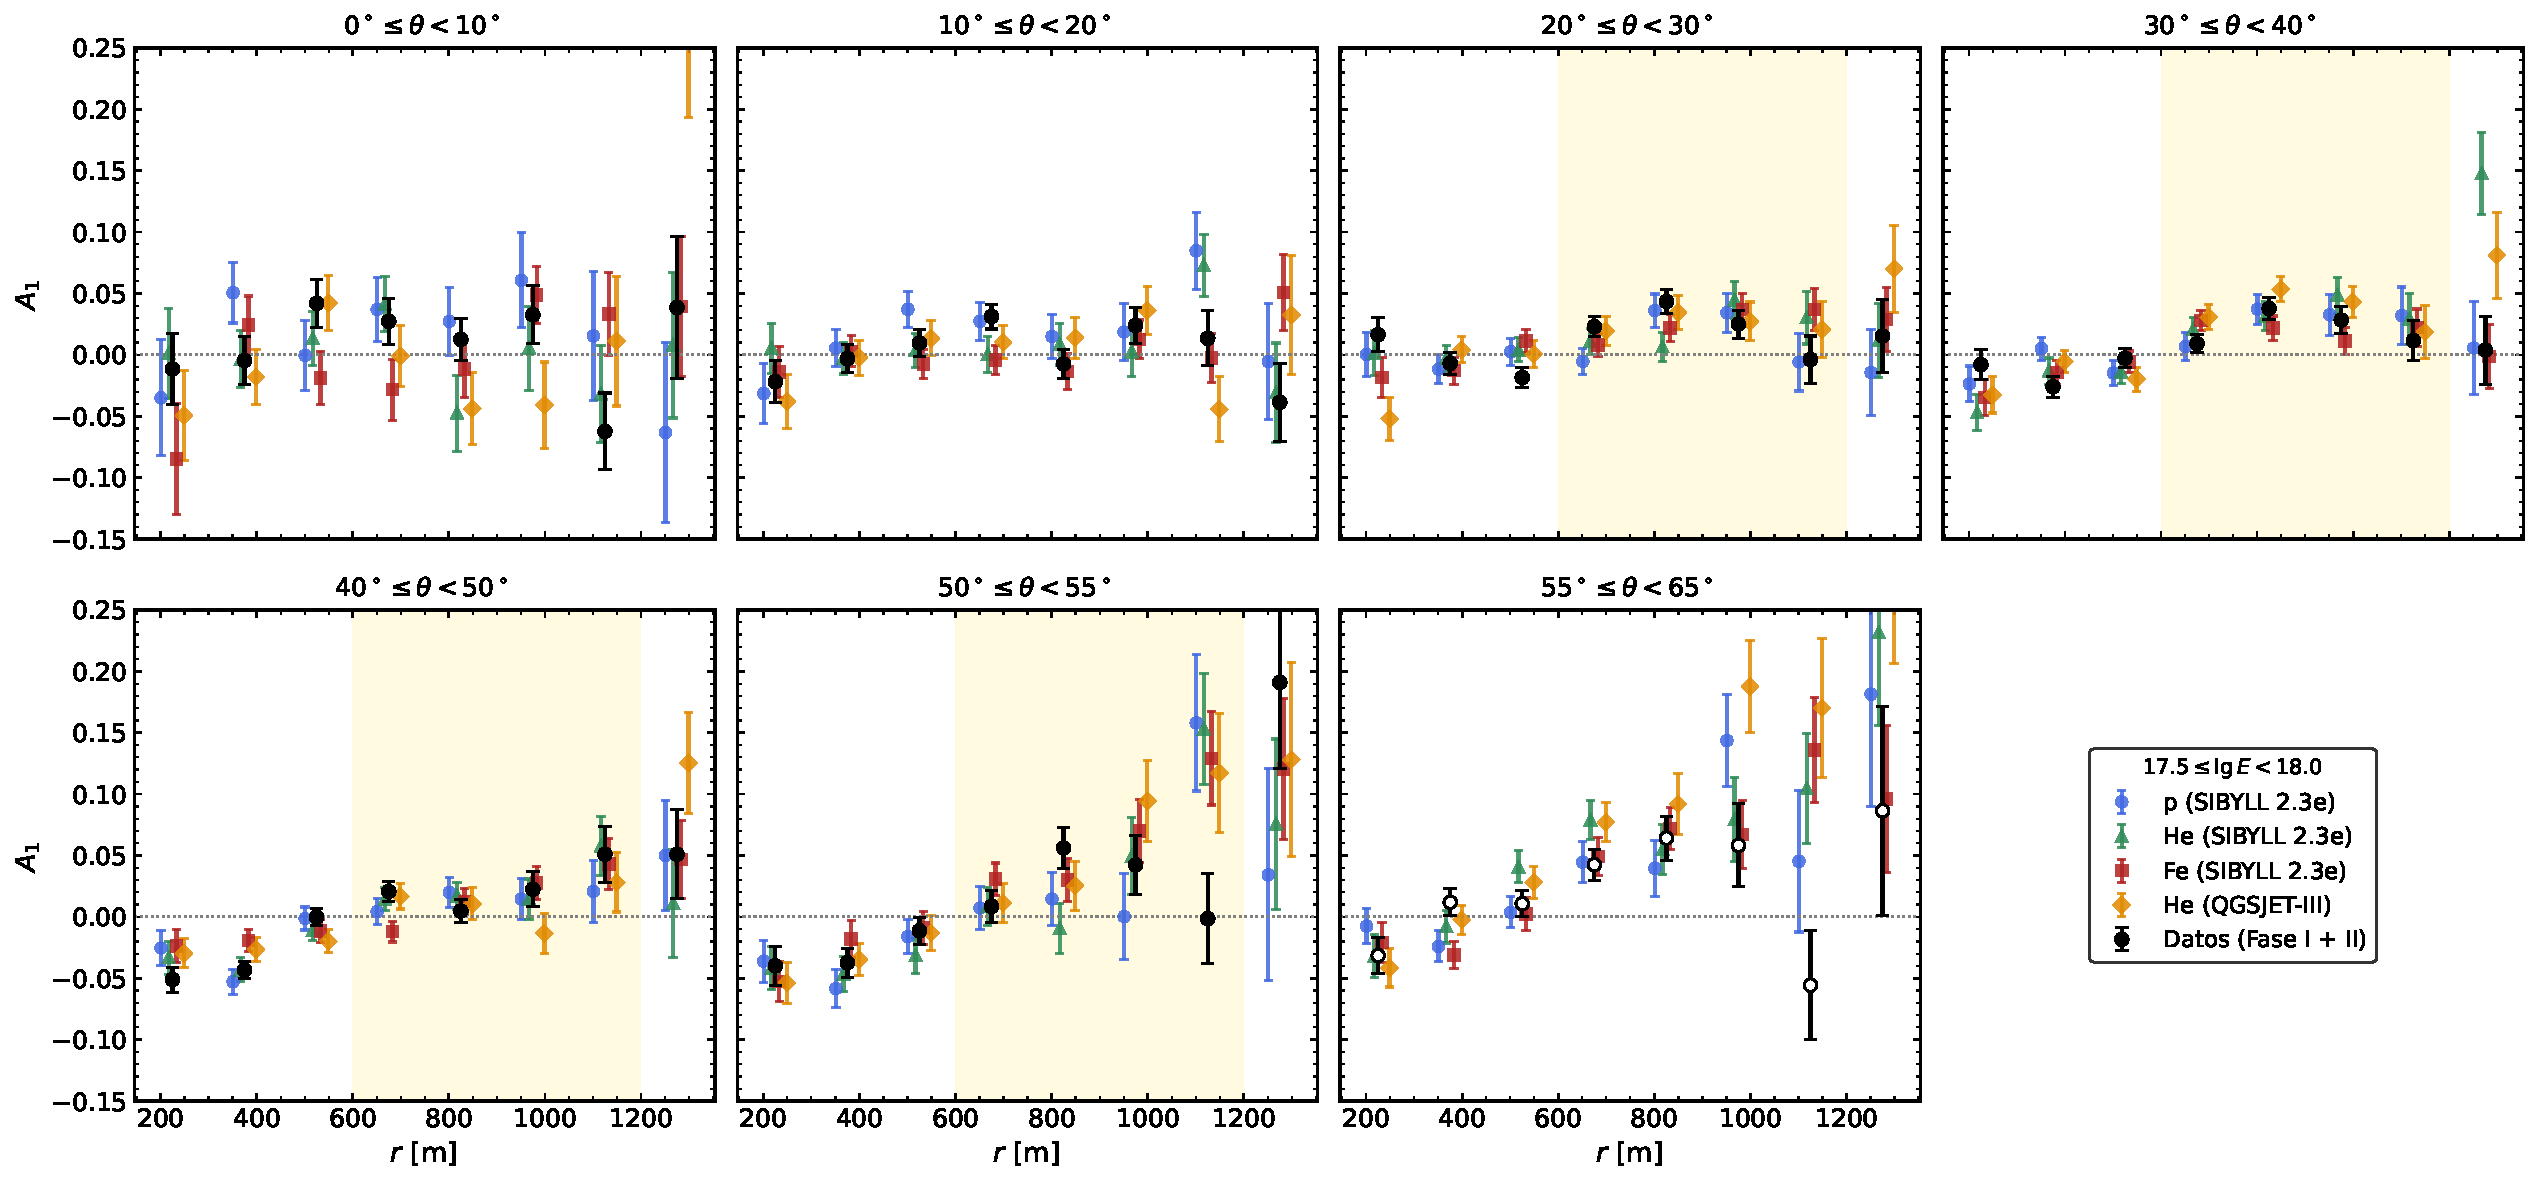
\includegraphics[width=\linewidth]{tesis/cap7_A1_vs_r_datos_vs_mc.pdf}\\
      {\footnotesize Datos (negro) frente a simulaciones reconstruidas,
      $17{,}5\le\lg E<18$.}
  \end{columns}
  \credito{Tesis, Cap.~6. Datos de campo: preliminar}
\end{frame}


\end{document}
